\documentclass[oneside]{book}

\usepackage{graphicx}
\usepackage{fancyhdr}
\usepackage{amsmath}
\usepackage{boxedminipage}
% \usepackage{tex/lineno}
\usepackage{lineno}
\usepackage{hyperref}


\newcommand{\grad}{\bigtriangledown}
\newcommand{\pd}{\partial}
\newcommand{\br}{\epsilon \mathcal{R}}



%%%%%%%%%%%%%%%%%%%%%%%%%%%%%%%%%%%%%%%%5
%
%  Set Up Margins

%%%%%%%%%%%%%%%%%%%%%%%%%%%%%%%%%%%%%%%%%%%%%%%%%
% include file for:
%      Critical Page setup dimensions
%            DO NOT MODIFY
%       (for help see "Latex Line by Line" p 260)
%
\setlength\oddsidemargin{0in}
\setlength\evensidemargin{0in}

\usepackage[left=0.98in, right=0.98in, top=1.0in, bottom=1.0in]{geometry}

% %Top Margin and header
% \setlength\voffset{-0.94in}
% \setlength\topmargin{0.25in}
% \setlength\headheight{0.25in}
% %\setlength\headwidth{6.5in}
% \setlength\headsep{0.25in}
% %Body
% \setlength\textwidth{6.5in}
% \setlength\textheight{9.50in}
% %Footer
% %\setlength\footheight{0.5in}
% \setlength\footskip{0.3750in}
% Line spacing for 6 lines per inch
\linespread{0.894}  % 1.0 = single    1.6 = double
%
%          END of Critical Page Setup Dimensions
%%%%%%%%%%%%%%%%%%%%%%%%%%%%%%%%%%%%%%%%%%%%%%%%%%%

%%%%%%%%%%%%%%%%%%%%%%%%%%%%%%%%%%%%%%%%%%%%%%%%%%%
%
% Useful style and math macros
%


\newcommand\Dfrac[2]{\frac{\displaystyle #1}{\displaystyle #2}}
\newcommand\beq{\begin{equation}}
\newcommand\eeq{\end{equation}}

\newcommand\bmat{\begin{bmatrix}}
\newcommand\emat{\end{bmatrix}}

\newenvironment{solution}
{\vspace{0.125in} {\bf SOLUTION:} \\ }
{\vspace{0.25in}}


% 
%%%%%%%%%%%%%%%%%%%%%%%%%%%%%%%%%%%%%%%%%%%%%%%%%
% include file for:
%      Critical Page setup dimensions
%            DO NOT MODIFY
%       (for help see "Latex Line by Line" p 260)
%
\setlength\oddsidemargin{0in}
\setlength\evensidemargin{0in}

\usepackage[left=0.98in, right=0.98in, top=1.0in, bottom=1.0in]{geometry}

% %Top Margin and header
% \setlength\voffset{-0.94in}
% \setlength\topmargin{0.25in}
% \setlength\headheight{0.25in}
% %\setlength\headwidth{6.5in}
% \setlength\headsep{0.25in}
% %Body
% \setlength\textwidth{6.5in}
% \setlength\textheight{9.50in}
% %Footer
% %\setlength\footheight{0.5in}
% \setlength\footskip{0.3750in}
% Line spacing for 6 lines per inch
\linespread{0.894}  % 1.0 = single    1.6 = double
%
%          END of Critical Page Setup Dimensions
%%%%%%%%%%%%%%%%%%%%%%%%%%%%%%%%%%%%%%%%%%%%%%%%%%%

%%%%%%%%%%%%%%%%%%%%%%%%%%%%%%%%%%%%%%%%%%%%%%%%%%%
%
% Useful style and math macros
%


\newcommand\Dfrac[2]{\frac{\displaystyle #1}{\displaystyle #2}}
\newcommand\beq{\begin{equation}}
\newcommand\eeq{\end{equation}}

\newcommand\bmat{\begin{bmatrix}}
\newcommand\emat{\end{bmatrix}}

\newenvironment{solution}
{\vspace{0.125in} {\bf SOLUTION:} \\ }
{\vspace{0.25in}}





%%%%%%%%%%%%%%%%%%%%00

%%%%%%%%%%%%%%%%%%%%%%%%%%%%%%%%%%%%%%%%%%%%%%%%%%%%%%
%
%  Example environment
%
\newcounter{Example}[chapter]

\newenvironment{Example}
{\refstepcounter{Example}\newpage
 \begin{boxedminipage}{\textwidth} % \linenumbers
    {\bf Example \thechapter.\theExample}\\
}
{\vspace{0.1in}\end{boxedminipage}
\vspace{0.4in} }

\newenvironment{ExampleCont}
{
 \begin{boxedminipage}{\textwidth}\linenumbers
    {\bf Example \thechapter.\theExample \hspace{4pt} cont.}\\
}
{\vspace{0.1in}\end{boxedminipage}
\vspace{0.4in} }


\newenvironment{ExampleSmall}
{\refstepcounter{Example}
 \begin{boxedminipage}{\textwidth}
    {\bf Example \thechapter.\theExample}\\
}
{\vspace{0.05in}\end{boxedminipage}
\vspace{0.25in} }
%
%%%%%%%%%%%%%%%%%%%%%%%%%%%%%%%%%%%%%%%%%%%%%%%%%%%%%

\def\bq{\begin{equation}}
\def\eq{\end{equation}}

% Symbol defs for equations
\def\ef{\mathcal{E}}
\def\fl{\mathcal{F}}

%
%%%%%%%%%%%%%   macros below are in ~/templates/pagedim.tex
% 
% \newcommand\Dfrac[2]{\frac{\displaystyle #1}{\displaystyle #2}}
% 
% %
% % %
% 
% \newcommand{\beq}[0]{\begin{equation}}
% 
% \newcommand{\eeq}[0]{\end{equation}}
% % %
%  \newcommand{\bmat}[0]{\begin{bmatrix}}
%  \newcommand{\emat}[0]{\end{bmatrix}}
% 
% \newenvironment{solution}
%  {\vspace{0.125in} {\bf SOLUTION:} \\ }
%  {\vspace{0.25in}}



\begin{document}
\setpagewiselinenumbers
\modulolinenumbers[5]

\setcounter{chapter}{0}


%  \frontmatter

 \title{EE543  Winter 2016\\Robot Manipulators}

 \author{Blake Hannaford}

 \date{\today\\(C) Copyright 2007-2016 Blake Hannaford}

 \maketitle

\tableofcontents

\mainmatter

\linenumbers

%  \part{Fundamentals}
%  Robotics Text  by Jacob Rosen and Blake Hannaford
% (c) 2007  Jacob Rosen and Blake Hannaford
%

\chapter{Introduction}
This text has evolved from lecture notes for EE543 at the University of Washington.  It will be evident to the reader that it is still very much a work in progress.  It owes a great deal to the book "Introduction to Robotics, Mechanics and Control," by John Craig.

As you read this book, please report typos or suggestions (by page and line number) to

{\tt https://catalyst.uw.edu/gopost/board/blake/20007/}

\section{Background and Motivational Examples}
 
\section{Definitions}

A robot manipulator is a chain of {\it links} connected by {\it joints}.
\subsection{Degree of Freedom}
A degree of freedom (DOF) is a motion which can be completely described by a scalar and its time derivatives. 

\subsection{Joints}
Joints constrain the relative position of two links in all but one degree of freedom. 

{\it Rotary } joints permit revolute motion about a line in space refered to as the motion axis. 

{\it Prismatic} joints  permit translational motion along a line in space refered to as the motion axis. 

Three key components of joints are actuators, sensors, and bearings.  

Actuators do work on the joint through the application of force or torque.  Most robot manipulators use electric motors as actuators but hydraulic, pneumatic, and other more exotic actuators can also be used. 

Sensors measure the motion of the degree of freedom of the joint and send this information to a control system.

Bearings are devices which restrict motion in all but one degree of freedom. They act as rigid structural elements in the constrained directions and minimize friction in the degree of freedom.

\subsection{End Effector}

The end effector of a robot is a device attached to a link in the chain (typically at the end of a serial chain) designed to accomplish a task.  Typical end effectors include grippers, spray guns, and tools.

\subsection{Joint Space}
\subsection{Task Space}
\subsection{Workspace}


\section{Fundamental Problems in Manipulator Control}

This book will use a large set of mathematical tools to model and analyze robot manipulators.  In learning all of these tools, it will be useful to keep in mind that all of them are used to answer fundamental and straightforward questions which must be answered in order to use robot manpipulators. 

\begin{itemize}
	\item Description of a positioning task

Q:  How do we specify the position and orientation of robot arms and objects?

A: Frames, Homogeneous Transformations, and joint-space teaching.

	\item Forward kinematics

Q: What is the position and orientation (configuration) of a robot end effector if joint positions are known?

A: A linear transformation (4x4 matrix) which is a function of the joint positions (angles, displacements) and specifies end effector configuration in the base frame.  This matrix can also map a point in the end effector frame to its representation in the base frame. 

	\item Inverse kinematics

Q: What joint positions $\theta$, do I need to achieve a given end effector configuration?

A: Form an equation by setting the 4x4 matrix of the foward kinematics problem equal to one specifiing the {\it desired} position and orientation.  Then solve this equation for the joint positions.   Be sure to watch out for existence of solutions and multiple solutions. 


	\item Velocity transformation


Q:  What joint velocities, $\dot{\theta}$, do I need to achieve a given velocity of the end effector (both linear and angular velocity) in all three dimensions of a convenient reference frame?

A: Compute the ``Jacobian Matrix", the matrix derivative, of the forward kinematic equations and invert it.   Watch out for singular matrix in which case the inverse does not exist.
\[
\dot{\theta} = J^{-1} \dot{x}
\]
 
	\item Force transformation

Q:  What joint torques, $\tau$, correspond to a given set of end effector forces and torques, $F$?

A: $\tau = J^T F$
 
	\item Inverse dynamics

Q: For a given motion, $\ddot{\theta}, \dot{\theta}, \theta(t)$, what are the required joint torques?


A:  We can derive a dynamic equation
\[
\tau(t) = M(\theta)\ddot{\theta} + C(\theta,\dot{\theta}) + g(\theta)
\]
by using the Recursive Newton-Euler or Lagrangian methods. 

	\item Position Control

Q: How can we command joint torques to achieve a desired end effector trajectory?

A: PID control, Feed-forward dynamic control (the method of computed torques).

	\item Force Control

Q: How can we command joint torques to achieve a set of forces and torques at the end effector?

A:  Open loop we can use $\tau = J^T F$. However because of friction and other losses in many typical manipulators we must use force sensing at the end effector and closed loop force control.


	\item Trajectory Generation

Q: If we know a trajectory we want to follow, how do we generate a time-function which is a quick but smooth and attainable trajectory between two configurations ``A" and ``B"?

A:  Methods include polynomial splines and trapezoidal velocity profiles.

	\item Motion Planning

Q:  How do we decide the path to take between two configurations ``A" and ``B"?

A:  Without considering obstacles, the most common approach is straight line interpolation.  When obstacles and joint limits must be considered this becomes the AI motion planning problem.

	\item Sensor Based Control

Q: How can I make use of non-joint sensor information (e.g. vision, proximity, etc.) to control robot motion (for example, to follow 1cm above an unknown surface).

A: Robot vision, vision servoing, sensor data fusion, world modeling, operational space control.

	\item Telemanipulation 

Q: How can a human operator control a remote manipulator in a ``natural" and productive way to achieve a task goal?

A: Generalized bi-lateral teleoperation.

\end{itemize}

\section{Summary of Notation}
% Summary of Notation for Chapter  01

This explains the notation of chapter 1.

%  \setcounter{chapter}{6}
 %  Robotics Text  by Jacob Rosen and Blake Hannaford
% (c) 2007  Jacob Rosen and Blake Hannaford
%

\chapter{Coordinate Transformations and Rigid Body Motions}

To properly control the manipulation of objects with robots, we must have precise and useful ways to describe their position and orientation.  In this chapter we start out with some definitions, and then develop the mathematical tools for this surprisingly non-straightforward task.   Finally we will combine position and orientation into a clever 4x4 matrix which represents both in one object.

%%%%** Section 1
\section{Problem Statement and Learning Objectives}
% Problem Statement and Learning Objectives for Chapter 02
\paragraph{Problem Statement}
 The problem this chapter addresses is to represent the position and orientation of rigid bodies and frames of reference in useful ways. 

\paragraph{Learning Objectives}
Upon completing this Chapter, the reader should be able to 
\begin{itemize}
	\item  Work with vectors and vector products.
	\item  Derive several mathematical represenations of 3D rigid body rotation
	\item  Represent any displacement and rotation of a rigid body by a 4x4 matrix (the homogeneous transformation).
        \item  Solve for unknown spatial relationships in terms of known spatial relationships using homogeneous transformations and transform graphs. 
\end{itemize}



%%%%** Section 2
\section{Description of Position and Orientation}

%%%%** Section 2.1
\subsection{Vectors and Translation}

We use vectors to represent the location of objects and also to represent translation movements from one point to another.


%
% \subsubsection{Unit Vector}
% \subsubsection{Difference between Vectors}
%%%%** Section 2.1.1
\subsubsection{Vector Cross Product}
We will sometimes need the vector cross product which is briefly defined here.

The cross product of two vectors, represented
\[
c = a \times b
\]
is a vector who's magnitude is
\[
|c| = |a||b|\sin(\theta)
\]
where $\theta$ is the angle between the two vectors.
and whos direction is orthogonal to both $a$ and $b$.  There are two orthogonal directions to $a$ and $b$ and the cross product sign is set by the right hand rule (sweeping the fingers from $a$ to $b$ and observing direction of thumb).   We will frequently consider the cross product of vectors separated by $90^\circ$ (for example the $X$ and $Y$ axes) and in this case
\[
|c| = |a||b|
\]

Another, equivalent, definition of the vector cross product can be expressed in matrix notation as
\[
a\times b = \left [
\begin{array}{ccc}
0 & -a_3 & a_2 \\
a_3 & 0 & -a_1 \\
-a_2 & a_1 & 0 \end{array} \right]
b
\]




\begin{ExampleSmall}
1) Find the magnitude of the cross product $a \times b$ where
\[
a = [ 3 \quad 4 \quad 7]^T \qquad \qquad  b = [ 2 \quad 4 \quad-3]^T
\]

\vspace{0.2in}

\[
c = a \times b
\]
\[
|c| = |a||b| = 8.6 \times 5.39 = 46.3
\]

2) Find the elements of the cross product.

\vspace{0.2in}
To get the components, it is easiest to use the matrix definition:
\[
c = \left [
\begin{array}{ccc}
0 & -7 & 4 \\
7 & 0 & -3 \\
-4 & 3 & 0 \end{array} \right]
\left [
\begin{array}{c}
2 \\ 4 \\ -3
\end{array}
\right ]        =
\left [
\begin{array}{c}
-40 \\ 23 \\ 4
\end{array}
\right ]
\]

You can verify that the magnitude of this vector is also 46.3.
\end{ExampleSmall}




%%%%** Section 2.2
\subsection{Coordinate Systems and Frames}

Of course when we use them numerically, our vectors must be defined with respect to axes in space.   Such a coordinate system contains three axes oriented to measure displacement in each of the three spatial dimensions.   We denote these axes $x,y,z$ and we will require that this system is {\it right handed} so that

\[
x \times y = z
\]
where $\times$ represents the vector cross product.
We can have as many coordinate systems as we like and they can differ from one another in two ways.  The location of their origin can be different, in which case we say they are {\it offset} or {\it displaced} from one another, and their orientation can be different, in which case we say they are {\it rotated} from one another.

 Another term for coordinate system is {\it reference frame} or simply {\it frame}.

%%%%** Section 2.3
\subsection{Points}
The numerical value or location of a point in space is only defined  with respect to a selected coordinate system.   Thus if we have a point, $P$, and a coordinate system, $A$, it will have a specific numerical location with respect to $A$. For example:
\[
^AP = \left [
\begin{array}{c}   1.7 \\ 0.25 \\ -3.1 \end{array}
\right ]
\]
While $P$ designates the point in the abstract, we add the leading subscript, $^AP$ to indicate $P$'s representation in coordinate system $A$.

The origin of a frame is also a point.   The displacement between two frames can thus be represented by a point, the origin of one frame, expressed in a second frame.   For example, imagine that  $M$ and $N$, are two coordinate systems not rotated with respect to each other, but their origins, $O_M$ and $O_N$, are separated by 5 cm in the x direction. Then
\[
^MO_N = [0.05  \quad 0.0 \quad 0.0]^T
\]
and
\[
^NO_M = [-.05 \quad 0.0 \quad 0.0]^T
\]




%%%%** Section 2.4
\subsection{Rigid Objects}
We will view rigid objects as a collection of points with a fixed relationship to one another.   How can we describe a rigid object's configuration in space with respect to some base frame, frame $B$?

%%%%** Figure 1
\begin{figure}
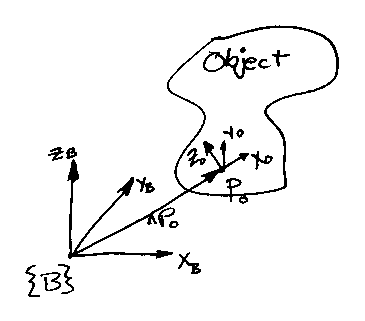
\includegraphics[width=3.5in]{figs02/00322.eps}
\caption{Representation of a rigid object in terms of an origin, $P_0$, and a frame attached to the object (frame $0$).}\label{ObjectLocationOrientation}
\end{figure}

First choose a point on the object, $P_0$ (Figure \ref{ObjectLocationOrientation}).    Then create a frame, $O$, whos origin is $P_0$.   The origin of $P_0$ does not have to be on or inside the object as long as all points in the object have a {\it fixed} representation in frame $O$.   The orientation of frame $O$ does not matter either as long as the previous condition is satisfied.   We can represent the location of the object in frame $B$ by simply the position of its origin, $^BP_0$.

Representation of the orientation of the object is somewhat more involved.   We can imagine that if we only know the location, $P_0$, the object is still free to rotate about $P_0$ in multiple ways.  Now, if we specify a second point on the object, $P_1$, the object is more constrained, but can still freely spin around the line connecting $P_0$ and $P_1$ without violating our assumption.  If we specify a third point on the object, we fully describe the object in both position and orientation.

We will be a little bit redundant and specify the object's configuration with four points:  the origin, $P_0$, and the tips of the three unit vectors of frame $O$:  $x_o$, $y_o$, $z_o$.   However we will remove the translation portion from these three points by subtracting $P_0$ to create
\[
\hat{x_0} = x_0 -P_0, \qquad \hat{y_0} = y_0-P_0,\qquad \hat{z_0} = z_0-P_0
\]

To capture the object's orientation, we represent these vectors in the base frame, frame $B$.
\[
^B\hat{x_0} = {^Bx_0} - {^BP_0} \quad \mathrm{etc.}
\]

Our representation of the object's configuration at this point is the tuple:

\[
^BObj = \left \{
\begin{bmatrix} ^BP_x \\ ^BP_y \\ ^BP_z \end{bmatrix},
\left [
\begin{array}{ccc}
\hat{^Bx_{Ox}}	&	\hat{^By_{Ox}}	&	\hat{^Bz_{Ox}} \\
\hat{^Bx_{Oy}}	&	\hat{^By_{Oy}}	&	\hat{^Bz_{Oy}} \\
\hat{^Bx_{Oz}}	&	\hat{^By_{Oz}}	&	\hat{^Bz_{Oz}} \\
\end{array}
\right]
\right \}
\]

we refer to the collection of $\hat{x_{O}}, \hat{y_O}, \hat{z_O}$ vectors into a matrix as a {\it rotation matrix.}.


%%%%** Section 3
\section{Rotation Matrix}\label{RotDefs}

We will study the rotation matrix from the point of view of four definintions.   Although these four definitions seem different at first, they are all simultaneously true. In this section we will consider only frames which differ in orientation.  We will add translation later.

The rotation matrix $^A_BR$  is:

\begin{enumerate}

	\item A matrix which specifies frame $B$ in terms of frame $A$.  The columns of $^A_BR$ are the unit vectors of frame $B$ specified in frame $A$.

	\item A matrix which maps a point expressed in frame $B$, $^BP$ to its representation in frame $A$, $^AP$, by matrix pre-multiplication:
\[
^AP = {}^A_BR \; ^BP
\]

	\item A description of an {\it operation} such as physically  turning from frame $A$ to frame $B$.

	\item A $3\times 3$ matrix with mathematical constraints:  If $R = [ a \quad b \quad c]$ where $a,b,c$ are 3-vectors, then
\[
|a| = |b| = |c| = 1
\]
and
\[
a \times b = c, \quad b \times c = a, \quad c\times a = b
\]
where $\times$ is the vector cross product.

\end{enumerate}

%%%%** Section 4
\section{Descriptions of Rotations}
There are many subtle aspects to rotation of objects and representing them mathematically.  In this section we will consider ways to describe rotations and combinations of rotations using the rotation matrix.


%%%%** Section 4.1
\subsection{Rotation in the Plane}

%%%%** Figure 2
\begin{figure}
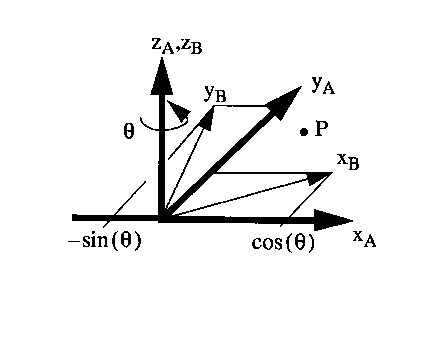
\includegraphics[width=3.5in]{figs02/00323.eps}
\caption{Two frames which are rotated relative to each other by the angle $\theta$ about the axis $z$.}\label{PlanarRotationFrames}
\end{figure}


Consider rotation in the $x,y$ plane about the axis $z$.  When we say ``about," we mean that any point along the line indicated by $z$ is unchanged by the rotation.  Also, the $z$ coordinate of any point is unchanged by rotation about the $z$ axis.  In Figure \ref{PlanarRotationFrames} we have two frames, $A$, in bold, and $B$.   $B$ is rotated about the $z$ axis with respect to $A$.   Consider the tip of the unit vector $x_A$.  After its rotation to $x_B$, it has components which we can project back on to $x_A$ and $y_A$.   It still has no component in $z$.   If we have rotated around $z$ by angle $\theta$, then these projections are
\[
^Ax_B = \left [ \begin{array}{c}   cos(\theta) \\ sin(\theta) \\ 0 \end{array} \right ]
\]
Similarly,

\[
^Ay_B = \left [ \begin{array}{c}   -sin(\theta) \\ cos(\theta) \\ 0 \end{array} \right ]
\]

These are two columns of the rotation matrix $^A_BR$:
\[
^A_BR = \left[
\begin{array}{ccc}
cos(\theta) & -sin(\theta) & ? \\
sin(\theta) &  cos(\theta) & ? \\
0           &          0   & ? \\
\end{array}\right]
\]


We can get column 3 of $^A_BR$ two ways.  First, as we have just done, we can note that
\[
^Az_B = {^Az_A} = \left[\begin{array}{c} 0 \\ 0 \\ 1 \end{array}\right]
\]
Therefore our complete matrix must be

\[
^A_BR = \left[
\begin{array}{ccc}
cos(\theta) & -sin(\theta) & 0 \\
sin(\theta) &  cos(\theta) & 0 \\
0           &          0   & 1 \\
\end{array}\right]
\]

A second way to complete the rotation matrix is to use definition 4, which specifies that the magnitude of each row or column must be one (Sec \ref{RotDefs}).  Thus
\[
|r_{31}|^2 = 1-\cos(\theta)^2-\sin(\theta)^2 = 0
\]
etc.

Our favorite point, $P$, has the representation $\{P_{XA}, P_{YA}\}$ in the $x,y$ plane.  $P_{ZA}$ can have any value for this discussion since our rotation is about $z$.
Just as it did with the unit vectors, $^A_BR$ maps $P$'s representation in $B$ to its representation in $A$:
\[
^AP = {^A_BR} \; {^BP}
\]
One way we can see this is by an argument of superposition since matrix multiplication is a linear transformation and $^BP$ can be expressed as a linear combination of the unit vectors of $B$.


%%%%** Sect
\subsection{Rotational Operators}
By similar arguments we can derive rotation matrices for rotation around the other axes, $x$, and $y$.  Let's denote the unit vectors,
\[
\hat{x} \equiv [1 \quad 0 \quad 0]^T \quad \hat{y} \equiv  [0 \quad 1 \quad 0 ]^T \quad \hat{z} \equiv [0 \quad 0 \quad 1]^T
\]
These are not vectors in any particular coordinate system, just the numerical values shown above.   We will define the matrices

\[
\mathrm{Rot}(\hat{x}, \theta) =  \left[
\begin{array}{ccc}
1  &     0        &      0    \\
0  &  \cos(\theta) & -\sin(\theta) \\
0  &  \sin(\theta) &  \cos(\theta) \\
\end{array} \right]
\]

\[
\mathrm{Rot}(\hat{y}, \theta) =  \left[
\begin{array}{ccc}
\cos(\theta)  &       0      & \sin(\theta) \\
     0       &       1      &     0       \\
-\sin(\theta) &       0      & \cos(\theta) \\
\end{array}\right]
\]

\[
\mathrm{Rot}(\hat{z}, \theta) =  \left[
\begin{array}{ccc}
\cos(\theta) & -\sin(\theta) & 0 \\
\sin(\theta) &  \cos(\theta) & 0 \\
0           &          0   & 1 \\
\end{array}\right]
\]



to designate rotations about the three main axes of a frame.   At this point let's introduce a shorter notation:

\[
c\theta \equiv cos(\theta), \quad s\theta \equiv sin(\theta)
\]
and
\[
c_1 = \cos(\theta_1), \quad s_1 = sin(\theta_1)
\]
for example,
\[
\mathrm{Rot}(\hat{x}, \theta_3) =
\left[
\begin{array}{ccc}
1  &  0  &  0    \\
0  & c_3 & -s_3  \\
0  & s_3 &  c_3  \\
\end{array}\right]
\]


\begin{ExampleSmall}
A point in frame $B$ is
\[
^BP = \left [ \begin{array}{c} -2 \\ 2 \\ 0.707 \end{array}\right]
\]
and there exists a frame $A$, whose rotation relative to $B$ is given by
\[
^A_BR = \mathrm{Rot} (\hat{x}, \pi/4 )
\]

1) What are the elements of $^A_BR$?

Answer:
\[
^A_BR = \left [ \begin{array}{ccc}
1  & 0 & 0  \\
0 & 0.707 & -0.707 \\
0 & 0.707 &  0.707 \end{array}\right]
\]

2) What is $^AP$?

Answer:
\[
^AP = ^A_BR{^BP} = \left[\begin{array}{c} -2.0 \\ 0.914 \\ 1.914 \end{array}\right]
\]

3) What is the change in magnitude of $P$ when it is rotated?

Answer:
\[
\frac{|^AP|}{|^BP|} = \frac{2.915}{2.915} = 1
\]


A rotation matrix should never change the magnitude of a point.
\end{ExampleSmall}



We can verify the fourth definition of the rotation matrix with the rotation operators. For example, using Rot($\hat{x}, \theta)$ we can easily verify that its columns have magnitude 1.   We can verify the cross product constraints as well. Using Rot($\hat{x}, \theta)$,  then let $a$ and $b$ equal the first two columns
\[
a = [1 \quad 0 \quad 0]^T, \quad b = [0 \quad c\theta \quad s\theta]^T
\]
We want to show that $a\times b=c$.
Recall that one definition of the vector cross product is
\[
a\times b = \left [
\begin{array}{ccc}
0 & -a_3 & a_2 \\
a_3 & 0 & -a_1 \\
-a_2 & a_1 & 0 \end{array} \right]
b
\]
so returning to our example,

\[
c = a \times b = \left [
\begin{array}{ccc}
0  & 0  & 0 \\
0  & 0 & -1 \\
0  & 1 & 0   \end{array} \right]
\left[ \begin{array}{c}
0 \\ c\theta \\ s\theta \end{array} \right]
=
\left[ \begin{array}{c}
0 \\ -s\theta \\ c\theta \end{array} \right]
\]

which is the answer we expect (i.e the third column of $\mathrm{Rot}(\hat{x},\theta)$) and  verifies that the third column is orthogonal to the first two.

%%%%** Section 4.2
\subsection{Inverse of a Rotation Matrix}

The properties given in our fourth definition describe an {\it orthonormal } matrix.   Any orthonormal matrix has an inverse which is equal to its transpose.  Thus for rotation matrices
\[
R^{-1} = R^T
\]
Clearly the inverse of a rotation matrix always exists because the transpose always exists.  When we apply this to  the coordinate transform application of rotation matrices:
\[
(^A_BR)^{-1} = (^A_BR)^T = ^B_AR
\]


%%%%** Section 4.3
\subsection{Composition of Rotations}\label{rotationorder}
Suppose there are two rotations which create a more complex relationship between two frames.  If we can transform a point from a rotated frame back to the base frame by premultiplying by the rotation matrix, then we should be able to do this twice to represent two rotations.




\begin{ExampleSmall}\label{RotExampLocalFrame}

Two frames, $A$, and $B$, start out coincident ($^A_BR = I$).  Then frame $B$ is rotated about $z_A$ by $\theta$ and then frame $B$ is rotated about $y_B$ by $\phi$.  Note that the second axis, $y_B$, is known in the most recent frame:
\[
^By_B = [0 \quad 1\quad 0]^T = \hat{y}
\]
.

1) What is $^A_BR(\theta,\phi)$?  In other words, what matrix represents the combination of both rotations?

Answer: Consider an intermediate frame, $A'$, to represent the frame after the first rotation:
\[
^A_{A'}R = \mathrm{Rot}(\hat{z}, \theta)
\]
by definition 3
\[
^{A'}_BR = \mathrm{Rot}(\hat{y},\phi)
\]
So now consider mapping a point in frame $B$, $^BP$, back to $A$ using definition 2 twice:
\[
^AP = {^A_{A'}}R {^{A'}_B}R ^BP
\]
Thus,
\[
^A_BR = \mathrm{Rot}(\hat{z},\theta)\mathrm{Rot}(\hat{y},\phi)
\]
\end{ExampleSmall}


We may combine successive rotations by {\it post}multiplication if each rotation is about a vector represented in the {\it current} rotated frame.
In  Example \thechapter.\ref{RotExampLocalFrame}, the first rotation, Rot$(\hat{z},\theta)$, is postmultiplied by the second rotation, $\mathrm{Rot}(\hat{y},\phi)$ to get the compound rotation $^A_BR$. This gives
\[
^A_BR(\theta, \phi) =
\left[
\begin{array}{ccc}
 c\theta & -s\theta & 0  \\
 s\theta &  c\theta & 0  \\
   0     &     0    & 1
\end{array}\right]
\left[
\begin{array}{ccc}
c\phi  & 0  & s\phi  \\
0      & 1  &   0    \\
-s\phi & 0  & c\phi
\end{array}\right]
=
\left[
\begin{array}{ccc}
c\theta c\phi       &     -s\theta      &  c\theta s\phi   \\
s\theta c\phi       &      c\theta      &  s\theta s\phi   \\
-s\phi              &         0         &   c\phi         \\
\end{array}\right]
\]




When successive rotations are described with respect to a single, fixed frame (in contrast to the compound example above), we may combine these by {\it pre}multiplication.   To illustrate this, we'll take the previous example of compound rotations and change just one thing:  the second rotation will take place around $y_A$ instead of $y_B$.




\begin{Example}\label{RotExampFixedFrame}

Two frames, $A$, and $B$, start out coincident ($^A_BR = I$).  Then frame $B$ is rotated about $z_A$ by $\theta$ and then frame $B$ is rotated about $y_A$ by $\phi$.  Unlike the previous example, the second axis is known only in the original frame, frame $A$. So we know:
\[
^By_A \ne [0 \quad 1 \quad 0]^T
\]


1) What is $^A_BR(\theta,\phi)$ this time?

\vspace{0.2in}

Answer: As before, consider the intermediate frame, $A'$, to represent the frame after the first rotation:
\[
{^A_{A'}}R = \mathrm{Rot}(\hat{z}, \theta)
\]
by definition 3 (Section \ref{RotDefs}).  For the second rotation let's use the point mapping interpretation, definition 2.  The second rotation must be represented by a matrix which maps a point from $B$ to $A'$.  This rotation is {\it not} one of our three cannonical rotation matrices because $y_A \ne \hat{y} $ in our current frame.   We can derive the proper transformation by breaking it down into three steps:


\begin{enumerate}
  \item Rotate (as  in physical move) $A'$ to $A$ using $^{^{A'}_{A}R}$.
  \item $\mathrm{Rot}(\hat{y},\phi)$
  \item Rotate back to $A'$ using $^{A}_{A'}R$.
\end{enumerate}
Thus,
\[
^{A'}_{B}R = \mathrm{Step\;1}\times\mathrm{Step\;2}\times\mathrm{Step\;3}
\]
\[
^{A'}_{B}R =  {{}^{A'}_A}R \; \mathrm{Rot}(\hat{y}, \phi) \; {}^A_{A'}R
\]

Now the complete mapping from $B$ to $A$ is
\[
{^A_B}R =  {^A_{A'}}R \; {^{A'}_B}R = {^A_{A'}}R \; {^{A'}_A}R \; \mathrm{Rot}(\hat{y}, \phi) \; {^A_{A'}}R
\]

Because ${^A_{A'}}R = {^{A'}_A}R^{-1}$, the first two rotation matrices cancel giving
\[
^{A}_BR = \mathrm{Rot}(\hat{y}, \phi)^A_{A'}R = \mathrm{Rot}(\hat{y}, \phi) \mathrm{Rot}(\hat{z}, \theta)
\]

expanding this:
\[
^A_BR = \begin{bmatrix} c\phi & 0 & s\phi \\ 0 & 1 & 0 \\ -s\phi & 0 & c\phi \end{bmatrix}
\begin{bmatrix}
c\theta      & -s\theta     &  0    \\
s\theta      &  c\theta     &  0    \\
   0         &     0        &  1
\end{bmatrix}
=
\begin{bmatrix}
c\phi c\theta     &  -c\phi s\theta    &  s\phi     \\
s\theta           &   c\theta          &  0         \\
-s\phi c\theta    &   s\phi c\theta    &  c\phi
\end{bmatrix}
\]

Note that after the cancelation, it is as though the second rotation {\it pre}multiplies the first one.

\end{Example}


\begin{Example}\label{RotExamp3Mixed}
Two frames $A$ and $B$ start out superimposed.  Then

\begin{quotation}

$B$ is rotated about $x_A$ by $\theta_1$.

$B$ is rotated about $y_B$ by $\theta_2$.

$B$ is rotated about $y_A$ by $\theta_3$.

\end{quotation}

What is $^A_BR$?

\vspace{0.2in}

Answer:

Set up intermediate frames as above:  $A', A''$.  Then
\[
^A_BR = {}^A_{A'}R \; ^{A'}_{A''}R \; ^{A''}_BR
\]

Considering the first rotation, since in the initial frame, $x_A = \hat{x}$ we can write
\[
^A_{A'}R = \mathrm{Rot}(\hat{x},\theta_1)
\]

In the second rotation, the axis is also known in the current frame: $^{A'}y_B=\hat{y}$, we can similarly write:
\[
^{A'}_{A''}R = \mathrm{Rot}(\hat{y},\theta_2)
\]

However for the third rotation we have to go all the way back to the initial frame:
\[
^{A''}_{B}R = \underbrace{
               ^{A''}_{A'}R \; ^{A'}_{A}R \; \mathrm{Rot}(\hat{y},\theta_3) \;  ^{A}_{A'}R \;^{A'}_{A''}R
               }
\]

Combining
\[
^A_BR = \underbrace{
     {}^A_{A'}R \; ^{A'}_{A''}R \;  ^{A''}_{A'}R \; ^{A'}_{A}R
     }_{=I}
\mathrm{Rot}(\hat{y},\theta_3) \;  ^{A}_{A'}R \;^{A'}_{A''}R
= \mathrm{Rot}(\hat{y},\theta_3) \;  ^{A}_{A'}R \;^{A'}_{A''}R
\]
\[
^A_BR = \mathrm{Rot}(\hat{y},\theta_3) \mathrm{Rot}(\hat{x},\theta_1) \mathrm{Rot}(\hat{y},\theta_2)
\]

\end{Example}


\begin{Example}

\begin{center}
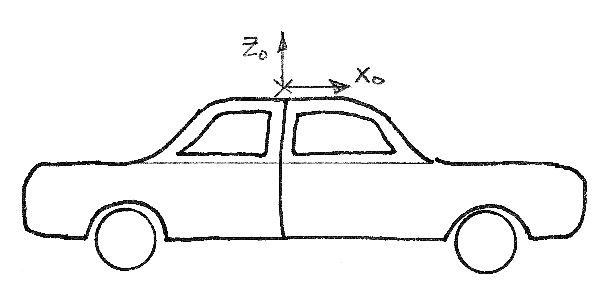
\includegraphics[width=3.5in]{figs02/00708.eps} ($\to$ front of car)
\end{center}
\vspace{0.2in}
A robotic car drives straight for 10 meters then turns right by $90^\circ$.  Then it drives up  a $45^\circ$ incline and comes to a stop.

A frame mounted to the top of the vehicle is called $F_0$.
The onboard computer can store the current value of $F_0$ at any time from navigation instruments as a 3x3 matrix.  Before driving the computer stores
\[
F_1 = F_0
\]
Then after the drive above, it stores the new orientation,
\[
F_2 = F_0
\]


What is the rotation matrix ${^1_2R}$ which describes the change in orientation?

Answer:

We have rotation matrices describing the three stages of the trip:

1) Drive straight for 10 meters:  $\begin{bmatrix}  1 & 0 & 0 \\ 0 & 1 & 0 \\ 0 & 0 & 1 \end{bmatrix}$

2) Turn right by $90^\circ$: Rot($\hat{z}$,  $-90^\circ$):  $\begin{bmatrix} 0 & 1 & 0 \\ -1 & 0 & 0 \\ 0 & 0 & 1 \end{bmatrix}$

3) Go up $45^\circ$ incline: Rot($\hat{y}, -45^\circ)$:  $\begin{bmatrix} 0.707 & 0  & -0.707 \\ 0 & 1 & 0 \\ 0.707 & 0 & 0.707 \end{bmatrix}$\\
(about the {\it local } frame).

Then we can combine them by postmultiplication:
\[
{^1_2R} = \begin{bmatrix}  1 & 0 & 0 \\ 0 & 1 & 0 \\ 0 & 0 & 1 \end{bmatrix}
\begin{bmatrix} 0 & 1 & 0 \\ -1 & 0 & 0 \\ 0 & 0 & 1 \end{bmatrix}
\begin{bmatrix} 0.707 & 0  & -0.707 \\ 0 & 1 & 0 \\ 0.707 & 0 & 0.707 \end{bmatrix}
\]
\[
{^1_2R} = \begin{bmatrix} 0 &  1 & 0 \\ -0.707 & 0 & 0.707 \\ 0.707 & 0 & 0.707 \end{bmatrix}
\]


\end{Example}

It can be confusing to remember the order of multiplication for multiple rotations.   One way to think about it is we always post-multiply successive rotations.  If the rotation is about the first, fixed frame, then we must use the similarity transformation as shown in Examples \ref{RotExampFixedFrame} and \ref{RotExamp3Mixed} of this chapter.  The effect of this similarity transformation is to make this appear like pre-multiplication.


To summarize, if we are careful, we can use the following rules of thumb to determine the order of matrix multiplication:

\begin{enumerate}
  \item  If the rotation is about an axis in the {\it original fixed  } frame, pre-multiply
  \item  If the rotation is about an axis in the {\it current} frame, post-multiply
\end{enumerate}



%%%%** Section 4.4
\subsection{Rotation of a Point}
The rotation matrix also describes the physical act of turning something (Figure \ref{RotationOfAPoint}).   So how can we describe the rotation of a point about an axis in a certain frame but still representing the point in the same frame?


%%%%** Figure 3
\begin{figure}
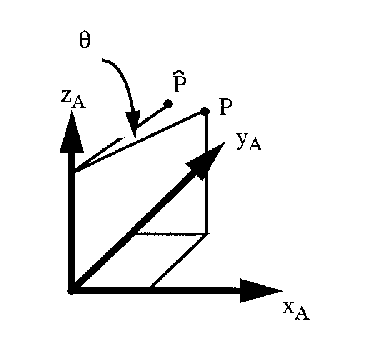
\includegraphics[width=3.0in]{figs02/00324.eps}
\caption{Rotation of a point around the $z$ axis by angle $\theta$.   Here we consider the point to actually move in a single frame, $A$. }\label{RotationOfAPoint}
\end{figure}

We consider the point's rotation to be positive if the angle from the orginal point, $P$, to the rotated point, $\hat{P}$, is positive in the right hand sense around the axis.  Consider for example, rotation of the point around the $\hat{z}$ axis.    By our third definition (Section \ref{RotDefs}),
\[
^A\hat{P} = \mathrm{Rot}(\hat{z},\theta)^AP
\]




%%%%** Section 4.5
\subsection{Rotations about axes other than $x,y,z$}
Suppose we have an arbitrarily rotated frame, F:
\[
F = {}^O_FR
\]
Geometrically, this might look like Figure \ref{ArbitraryRotation}.   Now we will use frame $F$ to study more general rotations.   Suppose $ ^O_FR$ is known and we want to do a rotation about $z_F$?  How do we represent a rotation about $z_F$ in frame $O$ by $\theta$?   Put another way, if the point $^OP$ is rotated about $z_F$ by $\theta$ to get $^O\hat{P}$, what is $^O\hat{P}$?

We solve this similarly to the last example by transforming back to frame $F$ and doing the canonical rotation about $\hat{z}$:
\[
^O\hat{P} = \;{}^O_FR \mathrm{Rot} \left (
\begin{bmatrix}  0 \\ 0 \\ 1 \end{bmatrix} , \theta \right )
 {}^F_OR
\]

\[
= \mathcal{R} \mathrm{Rot}(\hat{z},\theta)\mathcal{R}^T \; ^OP
\]
where $\mathcal{R} \equiv \;{}^O_FR$.
Another way to look at this is to define

\[
\mathrm{Rot}(z_F,\theta) = \mathcal{R} \mathrm{Rot}(\hat{z},\theta)\mathcal{R}^T
\]

Mathematically, this is a ``similarity transform" which can be used to rotate about an arbitrarily rotated vector, in this case, $z_F$.




%%%%** Figure 4
\begin{figure}
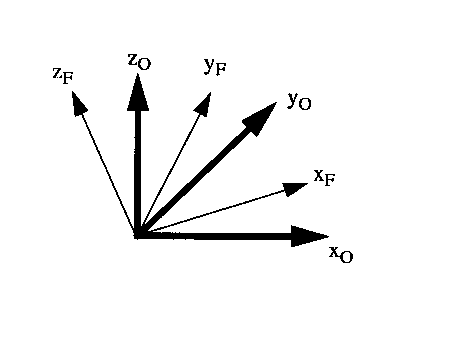
\includegraphics[width=3.5in]{figs02/00326.eps}
\caption{Frame $F$ has an arbitrary orientation relative to frame $O$}\label{ArbitraryRotation}
\end{figure}






%%%%** Section 5
\section{Three Parameter Representations of Rotation}
Although nine numbers are required to make a rotation matrix, only 3 of them are independent (this is because there are six constraints on the matrix in definition 4 of Section \ref{RotDefs}).  This implies that there should be representations of rotation needing only 3 parameters.


%%%%** Section 5.1
\subsection{Roll-Pitch-Yaw Angles (XYZ Fixed Angles)}

%%%%** Figure 5
\begin{figure}
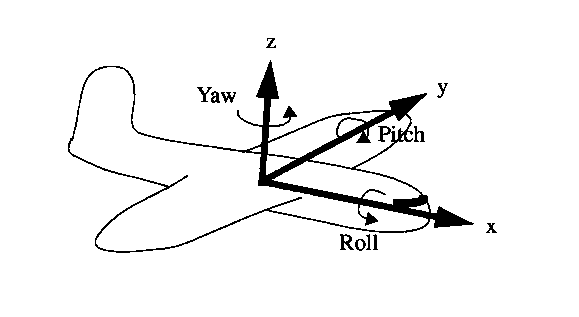
\includegraphics[width=3.5in]{figs02/00327.eps}
\caption{Roll-Pitch-Yaw angles (commonly used in avaition) describe rotations in a fixed order about $x,y,z$ axes of a fixed coordinate system.}\label{RollPitchYawFig}
\end{figure}

In aviation, aeronautics and sailing, the terms ``roll, pitch, and yaw" are commonly used.  These terms describe rotations about the $x,y,z$ axes of a fixed coordinate system in that order (Figure \ref{RollPitchYawFig}).  When we say that the coordinate system is ``fixed," we mean {\it not } that it is fixed to the object (i.e. the aircraft of Figure \ref{RollPitchYawFig}), but that its orientation is fixed in space.  Following the argument of Section \ref{rotationorder}, since these rotations are about a fixed frame, they should be combined by {\it pre-multiplication}:
\begin{equation}\label{RPYeqn}
R_{RPY} = \mathrm{Rot}(\hat{z}, Yaw)  \mathrm{Rot}(\hat{y}, Pitch)  \mathrm{Rot}(\hat{x}, Roll)
\end{equation}
If we define the amounts of Roll, Pitch, and Yaw, (positive in the right hand sense) about $x,y,z$ to be $C, B, A$ respectively, then
\[
R_{RPY} = \mathrm{Rot}(\hat{z}, A)  \mathrm{Rot}(\hat{y}, B)  \mathrm{Rot}(\hat{x}, C)
\]
\[
=
\begin{bmatrix}
 cA   & -sA  &  0    \\
 sA   &  cA  &  0    \\
 0    &   0  &  1
\end{bmatrix}
\begin{bmatrix}
cB    &  0   &  sB  \\
0     &  1   &  0   \\
-sB   &  0   &  cB
\end{bmatrix}
\begin{bmatrix}
 1    &  0   &   0  \\
 0    &  cC  &  -sC \\
 0    &  sC  &  cC
\end{bmatrix}
= \begin{bmatrix}
cAcB  &  cAsBsC-sAcC    &  cAsBcC+sAsC   \\
sAcB  &  sAsBsC+cAcC    &  sAsBcC-cAsC   \\
-sB   &  cBsC           &    cBcC
\end{bmatrix}
\]



%%%%** Section 5.2
\subsection{ZYX Euler Angles}\label{ZYXEuler}


Another 3-parameter representation which is commonly used is Euler Angles.
In this case the rotations are taken about the axes of a {\it rotating} frame.
Start with $F_1 = \{x_1,y_1,z_1\}$ superimposed on $F_0$.  Then rotate through the three steps labeled A-C in Figure \ref{ZYXEulerRotations}.

\begin{enumerate}
  \item Rotate about $z_0$ by $A$ to create $F_1$.
  \item Rotate about $y_1$ by $B$ to create $F_2$.
  \item Rotate about $x_2$ by $C$ to create $F_3$.
\end{enumerate}

By definition (3), step one defines $^0_1R$, step two defines $^1_2R$, etc.  By definition (2)
\[
^0_1R = \mathrm{Rot}(\hat{z},A) =
\mathrm{Rot} \left (
\hat{z} , A \right )
\]
maps a point in frame 1 to frame 0.
\[
^1_2R = \mathrm{Rot}(\hat{y},B) =
\mathrm{Rot} \left (
\hat{y} , B \right )
\]
maps a point in frame 2 to frame 1. And
\[
^2_3R = \mathrm{Rot}(\hat{x},C) =
\mathrm{Rot} \left (
\hat{x} , C \right )
\]
maps a point in frame 3 to frame 2.

Using the point mapping interpretation, the complete mapping is
\begin{equation}\label{ZYXEulerEqn}
^0_3R = ^0_1R\;^1_2R\;^2_3R = \mathrm{Rot}(\hat{z},A)\mathrm{Rot}(\hat{y},B)\mathrm{Rot}(\hat{x},C)
\end{equation}
Note that \eqref{RPYeqn} is the same as \eqref{ZYXEulerEqn}.   But, the Roll Pitch and Yaw angles are {\it not} equivalent to ZYX Euler angles, because the rotations $A$, $B$, and $C$ were applied in opposite orders in the two cases.  Specifically, for roll-pitch-yaw angles, we used $C$ for roll, but roll is applied {\it first} in the RPY method.
%%%%** Figure 6
\begin{figure}[h]
A 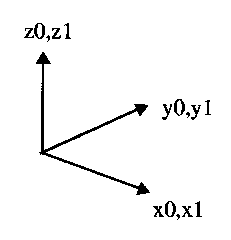
\includegraphics[width=1.0in]{figs02/00328.eps}
B 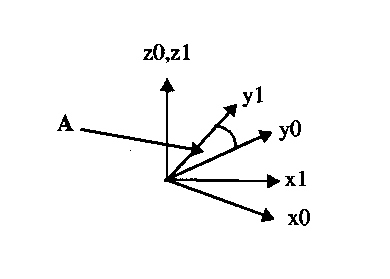
\includegraphics[width=1.5in]{figs02/00329.eps}
C 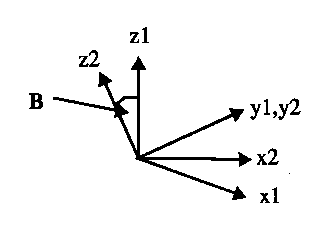
\includegraphics[width=1.5in]{figs02/00330.eps}
D 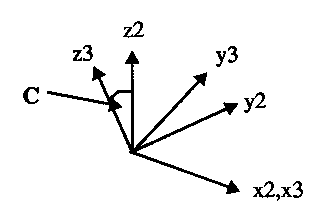
\includegraphics[width=1.5in]{figs02/00331.eps}
\caption{Initial Frames and rotations which make up the ZYX Euler Angles.}\label{ZYXEulerRotations}
\end{figure}
%
%
% %%%%** Section 5.3
% \subsection{ZYZ Euler Angles}
%
%
% (Similar material to previous subsection on ZYX Euler Angles)


%%%%** Section 6
\section{Equivalent Angle-Axis}\label{EquivAngleAxis}

Euler proved that any state of 3D rotation can be expressed by a single axis (i.e. a unit vector) and an amount of rotation.
Let the axis of rotation be
\[
K = [K_X\quad K_Y\quad K_Z]^T
\]
and the amount of rotation (in the right hand sense around $K$) be $\theta$,
then
\[
R_{K\theta} =
\begin{bmatrix}
K_X^2v\theta+ c\theta		& K_XK_Yv\theta-K_Zs\theta		&K_XK_Zv\theta+K_Ys\theta \\
K_XK_Yv\theta+K_Zs\theta	& K_Y^2v\theta+c\theta			&K_YK_Zv\theta-K_Xs\theta \\
K_XK_Zv\theta-K_Ys\theta	& K_YK_Zv\theta+K_Xs\theta		&K_Z^2v\theta+c\theta
\end{bmatrix}
\]
where
\[
v\theta = 1-\cos(\theta) \qquad c\theta = \cos(\theta) \qquad s\theta=\sin(\theta)
\]
Also, we require that $|K|=1$ to obtain a valid rotation matrix.   If implementing 
$R_{K\theta}$ in software, it is a good idea to normalize $K$ first as in:

\[
K = \frac{K}{|K|}
\]
so that we are sure it has magnitude 1. 

\begin{ExampleSmall}
Work out $R_{K\theta}$ for the special case of the $Z$ axis and compare the result to $rot(\hat{z}, \theta)$.

Let
\[
K = [0\quad0\quad1]^T
\]
Then setting $K_X$ and $K_Y$ to zero,
\[
R_{K\theta} =
\begin{bmatrix}
c\theta				& -K_Zs\theta				& 0 \\
K_Zs\theta			&     c\theta				& 0 \\
0				& 0					&K_Z^2(1-c\theta)+c\theta
\end{bmatrix}
\]
Since $K_Z=1$, this is equivalent to $rot(\hat{z}, \theta)$.
\end{ExampleSmall}


%%%%** Section 7
\section{Quaternions}\label{QuaternionSection}

% When we study Inverse Kinematics (Chapter \ref{xxxxxxxx}), we will see that there are difficulties with these three-parameter representations of rotation at certain configurations (for example when $B=0$).   An alternative is available which uses four parameters to represent orientation which has a  well defined representation for every orientation.   This alternative uses the notion of quaternions.

Another way to represent rotations of rigid bodies uses quaternions, a system like complex numbers which uses three ``imaginary" variables instead of just $i$.

To understand how a quaternion represents rotations, first consider basic complex numbers of the form $M = a+bi$.   The real and imaginary components of $M$ form a point in the complex plane.  For the purposes of rotation, we can assume that the magnitude of $M$ is 1 ($|M|=1$).  In polar form,
\[
|M| = \sqrt{a^2+b^2}  \qquad \angle{M} = \mathrm{atan2}(a,b)
\]

Remembering the rule ``Angles add, magnitudes multiply," or
\[
\angle(MN) = \angle(M) + \angle(N)
\]

Since $|M|= 1$, we can think of multiplying a complex number by $M$ as an operator which rotates the point to a new angle.
Electrical engineers will be familiar with this concept used to describe phase relationships between AC signals of the same frequency (phasors).

Quaternions can be thought of as a generalization of complex numbers using the symbols $i, j,$ and $k$, where
\[
i^2 = j^2 = k^2 = ijk = -1
\]
and where the multiplication of these elements is NOT commutitive (i.e. $ij \neq ji$).  The ``quaternion" has three imaginary components and one real component:
\[
q = a + bi+cj+dk
\]
The quaternion $q$ can also be thought of as the sum of a scalar ($a$) and a vector ($bi+cj+dk$).

Just as a complex number $M=a+bi$ has a complex conjugate, $M^* = a - bi$, quaternions have a quaternion conjugate

\begin{equation}\label{quaternioninversedefinition}
q^* = a - (bi+cj+dk)
\end{equation}

Just as a normal complex number can represent a rotation in the plane, quaternions can represent rotations in three dimensions.  The rotation is described by an axis of rotation, $K$, and a degree of rotation $\theta$.   As we saw above in Section \ref{EquivAngleAxis}, any rotation can be expressed this way as long as $\theta \neq 0$.

The well-known Euler's forumula for complex numbers is
\[
e^{i\theta} = \cos(\theta) + i\sin(\theta)
\]
The corresponding formula for quaternions is
\[
e^{\alpha(a_xi+a_yj+a_zk)} = \cos(\alpha) + (a_xi+a_yj+a_zk)\sin(\alpha)
\]
To use this to represent rotations we set $\alpha = \theta/2$.  Thus for an axis of rotation $K = (K_x, K_y, K_z)$
the quaternion representation of a rotation by $\theta$ around the axis $K$ is
\[
q = e^{\frac{\theta}{2} (K_xi+K_yj+K_zk)} = \cos(\theta/2) + (K_xi+K_yj+K_zk)\sin(\theta/2)
\]

The magnitude of $K$ is not used for rotation and often we require $|K|=1$.  The resulting quaternion is a unit quaternion.

To represent this quaternion without using $i,j,k$ (for example in some software), we just write down the four components

\begin{equation}\label{quaterniondefinition}
q = \cos(\theta/2) + K_xi\sin(\theta/2)+K_yj\sin(\theta/2)+K_zk\sin(\theta/2) = [w,x,y,z]
\end{equation}

\[
w = \cos(\theta/2) \qquad x =  K_x\sin(\theta/2) \qquad y = K_y\sin(\theta/2) \qquad z = K_z\sin(\theta/2)
\]
\begin{equation}\label{quaternioncomponents}
q = [w,x,y,z]
\end{equation}

Multiplication of quaternions is best left to the computer!  If two quaternions are given by
\[
q_1 = a_1 + b_1i + c_1j + d_1k \qquad q_2 = a_2 + b_2i + c_2j + d_2k
\]
Their product is
\begin{equation}\label{quaternionproduct}
q_{12} =
 a_1a_2-b_1b_2-c_1c_2-d_1d_2 +
(a_1b_2+b_1a_2+c_1d_2-d_1c_2)i +
(a_1c_2-b_1d_2+c_1a_2+d_1b_2)j +
(a_1d_2+b_1c_2-c_1b_2+d_1a_2)k
\end{equation}
or equivalently
\[
q_{12} =   \begin{array}{ccc}
[ a_1a_2-b_1b_2-c_1c_2-d_1d_2, &
(a_1b_2+b_1a_2+c_1d_2-d_1c_2),&
(a_1c_2-b_1d_2+c_1a_2+d_1b_2),\\
\qquad (a_1d_2+b_1c_2-c_1b_2+d_1a_2) ]
\end{array}
\]
whenever we write the product of two quaternions (i.e. $q_1q_2$) we refer to this computation (which, like matrix multiplication, is not commutative).


The quaternion can be expressed as a rotation matrix as follows

\[
R(q) =  \begin{bmatrix}
 c\theta	+ K_x^2(1-c\theta)	&  K_xK_y(1-c\theta) -K_zs\theta 	&  K_xK_z(1-c\theta)+K_ys\theta \\
K_yK_x(1-c\theta)+K_zs\theta	&  c\theta+K^2_y(1-c\theta)       &  K_yK_z(1-c\theta)-K_xs\theta   \\
K_zK_x(1-c\theta)-K_ys\theta	&  K_zK_y(1-c\theta)+K_xs\theta	&  c\theta+K_z^2(1-c\theta)      \\
\end{bmatrix}
\]
where $s\theta = \sin(\theta)$ and $c\theta = \cos(\theta)$.
Equivalently, for $q = [w,x,y,z]$,

\[
R(q) = \begin{bmatrix}
1-2y^2-2z^2	& 2(xy-wz)	& 2(wy+xz)	\\
2(wz+yx)	& 1-2x^2-2z^2	& 2(yz-xw)	\\
2(xz-wy)	& 2(yz+xw)	& 1-2y^2-2x^2
\end{bmatrix}
\]

Since each quaternion corresponds to a rotation matrix, combining successive rotations represented by quaternions should be done in the same order as combining rotation matrices.   I.e. if the next rotation is expressed as a quaternion in the local coordinate system, post-multply and if it is expressed in a fixed original coordinate system, pre-multiply.

\begin{ExampleSmall}\label{quaternionmultiplication}
Two frames $A$ and $B$, are initially aligned.  Frame $B$ is first rotated by $30^\circ$ about the vector $[0.371, 0.557, 0.743]$.
Then Frame $B$ is further rotated by $45^\circ$ about the vector $[0.684, 0.570, 0.456]$ (in the current frame).  Find the quaternion representing the complete rotation.

\[
q_1 = [ \cos(15^\circ), \quad 0.371\sin(15^\circ), \quad 0.557\sin(15^\circ), \quad 0.743\sin(15^\circ)]
\]
\[
q_2 = [ \cos(22.5^\circ), \quad 0.684\sin(22.5^\circ), \quad 0.570\sin(22.5^\circ), \quad 0.456\sin(22.5^\circ)]
\]
\[
q_{12} = q_1q_2
\]
Using the computer:
\[
q_1 = [0.966, 0.096, 0.144, 0.193] \qquad  q_2 = [0.924, 0.262, 0.218, 0.174]
\]
\vspace{0.1in}
\[
q_{12}= q_1q_2 = [0.802 \quad 0.325, \quad 0.377 \quad 0.330]
\]

\end{ExampleSmall}

\begin{ExampleSmall}


A rotation is to be performed about the vector $Rv = (0,1,0)$ by $45^\circ$.    Compute the quaternion to represent this rotation, and express it as a Rotation matrix.

\vspace{0.1in}

First, $\theta$ = $45^\circ$, and the axis of rotation, $K = [0,1,0]$, so using equation \ref{quaternioncomponents},

\[
q = [\cos(\theta/2), \quad 0\sin(\theta/2),\quad 1\sin(\theta/2),\quad 0\sin(\theta/2) ]
\]
\[
q = [.924, \quad 0, \quad .383, \quad 0]
\]
Using either matrix form above,
\[
R(q) = \begin{bmatrix}
0.707   &  0  &  0.707   \\
0       &  1  &  0       \\
-0.707   &  0  &  0.707   \\
\end{bmatrix}
\]

Which is the expected result since $q$ represents a rotation of $45^\circ$ about the $y$ axis.
\end{ExampleSmall}


\begin{Example}
Using the quaternions $q_1$ and $q_2$ from Example \thechapter.\ref{quaternionmultiplication}, Compute their two rotation matrices, multiply them together, and compare the result with the matrix version of $q_{12}$ from Example \thechapter.\ref{quaternionmultiplication}.

\vspace{0.1in}

First, convert $q_1$, $q_2$ to rotation matrices:
\begin{verbatim}

-->Ra = quat2rot1(qtimes(q1,q2))
 Ra  =

    0.4988392  - 0.2837947    0.8199695
    0.7742173    0.5728992  - 0.2723774
  - 0.3917614    0.7701054    0.5051711

-->Rb = quat2rot1(q1) * quat2rot1(q2)
 Rb  =

    0.4987583  - 0.2839447    0.8202152
    0.7744610    0.5728083  - 0.2725517
  - 0.3919257    0.7703584    0.5050751

\end{verbatim}

Comparing the results we see that the two matrices are nearly identical. More precisely, we can subtract the two matrices and find the maximum absolute error:
\begin{verbatim}

-->max(abs(Rb-Ra))
 ans  =

    0.0002530

\end{verbatim}
Since the columns and rows of rotation matrices must have magnitude 1, we can see that this error is very small.
\end{Example}


The inverse of a rotatation is the conjugate of the corresponding quaternion.  If $q$ is defined as in equation (\ref{quaterniondefinition}), then

\[
q^* = \cos(\theta/2) - K_xi\sin(\theta/2) -K_yj\sin(\theta/2) - K_zk\sin(\theta/2) = [w,-x,-y,-z]
\]


To use a quaternion for rotation of a point, if we define a point $P_1 = (P_x,P_y,P_z)$.  To rotate it around axis $K$ by $\theta$, let
\[
q_1 =  \cos(\theta/2) + (K_xi+K_yj+K_zk)\sin(\theta/2)
\]
and then
\begin{equation}\label{quaternpointrotation}
P_2 = q_1\hat{P}q_1^*
\end{equation}
where
\[
\hat{P} = [0,\; P_X,\; P_Y,\; P_Z]
\]
and the products are formed by quaternion-style multiplication.


\begin{ExampleSmall}
A rotation defined by a $63^\circ$ rotation about the axis $[-0.349, 0.814, 0.465]$ is applied to the point,
$P2 = [52.3, 67.0, -48.72]$.   Find the new point using quaternions and compare it with the equivalent angle-axis method.

\vspace{0.2in}

Using equation \thechapter.\ref{quaternpointrotation},
\begin{verbatim}
-->q4=quaternion([-.349,.814, .465], 63)
 q4  =

    0.8526402
  - 0.1822953
    0.4251816
    0.2428863

-->P2=[52.3,67,-48.72]
 P2  =

    52.3    67.  - 48.72

--> P2a = qtimes(q4, qtimes([0,P2],qcomp(q4)))
 P2a  =
    0.
  - 41.927377
    42.98847
  - 77.408106

// check by matrix rotation of point P2

-->R=quat2rot1(q4)
 R  =

    0.5204537  - 0.5692065    0.6364998
    0.2591720    0.8155493    0.5174062
  - 0.8136079  - 0.1043230    0.5719780

-->R*P2'
 ans  =
  - 41.927377
    42.98847
  - 77.408106

\end{verbatim}
\end{ExampleSmall}









%%%%** Section 8
\section{Side Topic:  Rotations in higher dimensions}
We have seen that at least three parameters are sufficient and necessary to specify rotation in three dimensions.   Is it a coincidence that 3 dimensional space has 3 rotation parameters?    Any hope for this simple rule is dashed by considering that only 1 orientation parameter is needed in 2 dimensions.   How many parameters are required to specify rotations of a 4 dimensional object?

We will use definition 4 to rephrase and generalize the question:  How many parameters does it take to specify an $n\times n$ orthonormal matrix?

The total number of matrix elements is $n^2$.   Then there are two sets of constraints:

\begin{enumerate}
  \item  $C_i \cdot C_j = 0$
  \item $|C_i| = 1$
\end{enumerate}
where $C_i$ is the $i$th column of the matrix.

The number of constraints due to the first condition is
\[
\binom{n}{2} = \frac{n!}{2(n-2)!}
\]
and the number of constraints of the second type is $n$.  So the total number of parameters is the number of matrix elements minus the number of constraints:
\[
N = n^2 - \frac{n!}{2(n-2)!}
\]
which can be simplified to
\[
N = \frac{1}{2} (n^2-n)
\]
So for a four dimensional object we need 6 parameters and for a 10 dimensional one we need 45 parameters(!).








%%%%** Section 9
\section{Homogeneous Transformation}
Considering several nice properties of the Rotation Matrix, in this Section, we will
find a  way to add translation to our matrix description of the configuration of a rigid object.
Earlier we used the $x,y,z$ coordinates of the origin of a frame attached to an object, with the rotation matrix of that frame,  to have its configuration completely specified  relative to some ``base frame," $B$ i.e.
\[
\mathrm{configuration} = \{^Bx,^By,^Bz, {}^B_0R\}
\]

More generally, this gives us a way to relate frames to each other.   Suppose we have a series of frames with different positions and orientations, and some relations between them as in Figure \ref{ThreeFramesVectors}.





%%%%** Figure 7
\begin{figure}
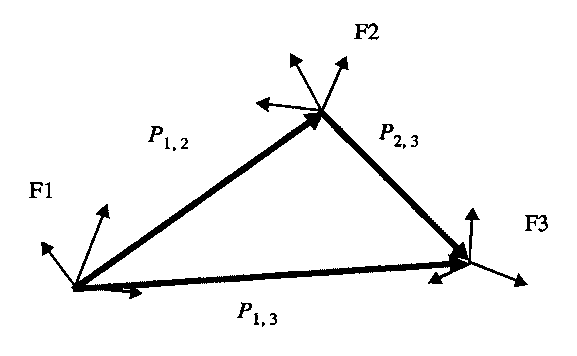
\includegraphics[width=3.5in]{figs02/00332.eps}
\caption{Three frames which are offset from each other in position and orientation. Vectors show displacements between the origins of the frames.}\label{ThreeFramesVectors}
\end{figure}



We can pose the following questions about these three frames:

If we know $P_{1,2}, P_{2,3}, \;^1_2R, \; ^2_3R$, what is $P_{1,3}, \;^1_3R$?

Consider a point expressed in frame 3, $^3P$.  It can be expressed in frame 2 by the affine transformation
\[
^2P = P_{2,3}+ \;{}^2_3R \;{}^3P
\]
and in frame 1 by
\[
^1P = P_{1,2} + \;{}^1_2R(P_{2,3}+ \;{}^2_3R \;{}^3P)
\]
Equivalently,
\[
^1P = \underbrace{P_{1,2} + ^1_2RP_{2,3}}{}+ \underbrace{^1_2R\;^2_3R}{} ^3P
\]
from which we can conclude
\[
P_{1,3} = P_{1,2} + ^1_2RP_{2,3} \qquad  ^1_3R = \;{}^1_2R\;^2_3R
\]


Although the preceding can be used as a general way to represent the spatial relationships between objects and robots, it is messy because we must add as well as multiply.  This is a problem because we often have to represent a series of these transforms which yields ever more complicated expressions.

An alternative is presented by ``homogeneous coordinates" which cleverly use an additional dimension to reduce the affine transformation to pure matrix multiplication.  We define the homogeneous transform
\[
^1P = \;{}^1_2T^2P
\]
where
\[
^1_2T =
\begin{bmatrix}
\begin{bmatrix}  &  &  \\  & ^1_2R&  \\ & & \\ \end{bmatrix}      &
 \begin{bmatrix}  \\ ^1P_{1,2} \\  \\ \end{bmatrix}            \\
 0 \quad 0 \quad 0      &   1
\end{bmatrix}
\]

This $4\times4$ matrix compactly describes both the rotation and the position offset.  When we work with homogeneous transforms, we augment our position vectors by adding a 1 in the fourth position. i.e.
\[
^1P = \begin{bmatrix} ^1P_x \\^1P_y \\ ^1P_z \\ 1 \end{bmatrix}
\]
in the example above,
\[^1P = ^1_2T^2P =
\begin{bmatrix}
\begin{bmatrix}  &  &  \\  & ^1_2R&  \\ & & \\ \end{bmatrix}      &
 \begin{bmatrix}  \\ ^1P_{1,2} \\  \\ \end{bmatrix}            \\
 0 \quad 0 \quad 0      &   1
\end{bmatrix}
\begin{bmatrix} ^2P_x \\^2P_y \\ ^2P_z \\ 1 \end{bmatrix}
\]
\[
= \begin{bmatrix}
^1_2R_{[1]}\cdot{}^2P+\;{}^1P_{{1,2}_{[1]}} \\
^1_2R_{[2]}\cdot{}^2P+\;{}^1P_{{1,2}_{[2]}} \\
^1_2R_{[3]}\cdot{}^2P+\;{}^1P_{{1,2}_{[3]}} \\
1\\
\end{bmatrix}
=
\begin{bmatrix}
^1P_{1,2}+ \;{}^1_2R \;{}^2P \\ 1 \\
\end{bmatrix}
\]

where $^1_2R_{[i]}$ represents row $i$ of $^1_2R$, and $^2P+\;{}^1P_{{1,2}_{[i]}}$ represents the $i$th element of $^1P_{1,2}$.
Notice that the final expression is completely equivalent to multiplying by a rotation matrix and then adding a translation.

With homogeneous transformations at our disposal, a series of spatial replationships can be expressed by a series of matrix multiplications as with pure rotation.  For example, solving the problem posed above for the three frames, $F1, F2, F3$,
\[
^1_3T = \; {}^1_2T\;^2_3T
\]
which is more compact indeed.

\paragraph{Homogeneous Transformation Definitions}\label{HTDefs}
The homogeneous transformation has definitions analogous to those we made for rotation:


The homogeneous transformation $^A_BT$ is

\begin{enumerate}
  \item A matrix which specifies frame $B$ in terms of frame $A$.
  \item A matrix which maps a point represented in frame $B$, $^BP$, to its representation in frame $A$, $^AP$.
  \item A description of an operator, perhaps corresponding to a physical move, {\it from} frame $A$, {\it to} frame $B$.
  \item A $4\times 4$ matrix with the structure given above.
\end{enumerate}


\begin{Example}
\begin{center}
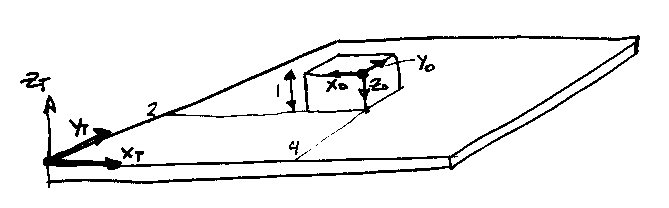
\includegraphics[width=4.5in]{figs02/00333.eps}
\end{center}

Find the $4\times 4$ homogeneous transformation which represents the configuration of the box on the table.   Frame $0$ is placed on a corner of the box and frame $T$ is at a corner of the table such that $X_T$ and $Y_T$ are in the plane of the table top.

Question:  What is $^T_0T$?

Answer:  First, find the translation offset between the origin of the box frame ($O$) and the table frame ($T$):
\[
^TP_O = \begin{bmatrix} 4 \\ 2 \\ 1 \end{bmatrix}
\]
Then, identify the rotation matrix.  First, align the frames by redrawing frame $O$ without the offset superimposed on $T$.  Then write each column of $^T_OR$.  Each column is the vector $\{x_O, y_O, z_O\}$ written in frame $T$:
\[
^T_OR = \begin{bmatrix}
-1 & 0 & 0 \\
0 & 1 & 0  \\
0 & 0 & -1 \\
\end{bmatrix}
\]
The homogeneous transform is thus:
\[\begin{bmatrix}
 -1   &   0  &  0  &  4  \\
  0   &   1  &  0  &  2  \\
  0   &   0  &  -1 &  1  \\
  0   &   0  &   0 &  1  \\
\end{bmatrix}
\]
\end{Example}

\begin{Example}

\includegraphics[width=4.5in]{figs02/00578.eps}

Two frames are on a conveyor belt.  We have the following facts about the system
\begin{itemize}
  \item The belt runs at 0.5 meters/sec.
  \item The belt is in the $\{X_0,Y_0\}$ plane.
  \item The belt is oriented $45^\circ$ from the $X_0$ axis as shown in the ``Top View".
  \item The origin of Frame $F_1$ is aligned with the origin of $F_0$ at $t=0$.
  \item Frame $F_1$ moves with the belt but Frame $F_0$ does not.
  \item $X_1$ is pointing along the belt (same direction as belt velocity.)
\end{itemize}

Find the 4x4 homogenous transform (which is a function of time) of $F_1$

Answer:

$O$:  The origin of $F_1$ is a function of time moving along the belt.
\[
O = \begin{bmatrix} 0.5t \cos(45^\circ) \\ 0.5t\sin(45^\circ) \\ 0 \end{bmatrix} = [0.35t, \quad 0.35t, \quad 0]^T
\]
Rotation = $rot(\hat{z}, 45^\circ)$
\[
\begin{bmatrix} 0.707 & -0.707 & 0 \\ 0.707 & 0.707 & 0 \\ 0 & 0 & 1 \end{bmatrix}
\]
\[
{^0_1T} = \begin{bmatrix} 0.707 & -0.707 & 0 & 0.35t \\ 0.707 & 0.707 & 0 & 0.35t \\ 0 & 0 & 1 & 0 \\ 0 & 0 & 0 & 1 \end{bmatrix}
\]
\end{Example}


%%%%** Section 9.1
\subsection{Inverse of Homogeneous Transforms}

We will frequently need the inverse of the 4x4 homogeneous transform matrix.   It seems intuitive that this inverse always exists because physical rotations and translations can always be ``undone."   It is straightfoward to derive the inverse of the 4x4 homogeneous transform,

Consider mapping a point in frame $B$ to its value in frame $A$ with both translation and rotation:
\[
^AP = {^A_BT}{^BP} = {^AO} + {^A_BR}{^BP}
\]
Where ${^AO}$ is the origin of frame $B$ expressed in $A$.
To invert this we seek a 4x4 matrix, $({^A_BT})^{-1}$ such that
\[
{^BP} = ({^A_BT})^{-1} {^AP}
\]

Solving
\[
{^BP} = ({^A_BR})^{-1}({^AP}-{^AO})
\]
\[
= {^B_AR} \; {^AP}-{^B_AR}\;{^AO}
\]
% Thus,
% \[
% T  =
% \begin{bmatrix}
% \begin{bmatrix}  &  &  \\  & R &  \\ & & \\ \end{bmatrix}      &
%  \begin{bmatrix}  \\  P \\  \\ \end{bmatrix}            \\
%  0 \quad 0 \quad 0      &   1
% \end{bmatrix}
% \]
% is
\[
{^A_B}T^{-1} =
\begin{bmatrix}
\begin{bmatrix}  &  &  \\  & {^A_BR}^T &  \\ & & \\ \end{bmatrix}      &
 \begin{bmatrix}  \\ -{^A_BR}^T {^AO} \\  \\ \end{bmatrix}            \\
 0 \quad 0 \quad 0      &   1
\end{bmatrix}
\]

You can verify this by showing that $TT^{-1} = I_{4\times4}$.


%%%%** Section 10
\section{Transform Equations}

It is useful to develop a slightly more formal description of the relationships
between frames.
Spatial relationships can be expressed as transforms, products of
transforms, or transform graphs. Transform graphs are directed
graphs. Links specify transform matrices between frames. We represent
a transform between two frames A, and B, by

\[
A \to B
\]
The arrow above is a graphical representation of $^A_BT$ and also of $^B_AT^{-1}$.
A series of links (a path) in the transform graph corresponds to {\it post}
multiplication of the transforms in the direction of the path.

%%%%** Figure 8
\begin{figure}[h]\centering
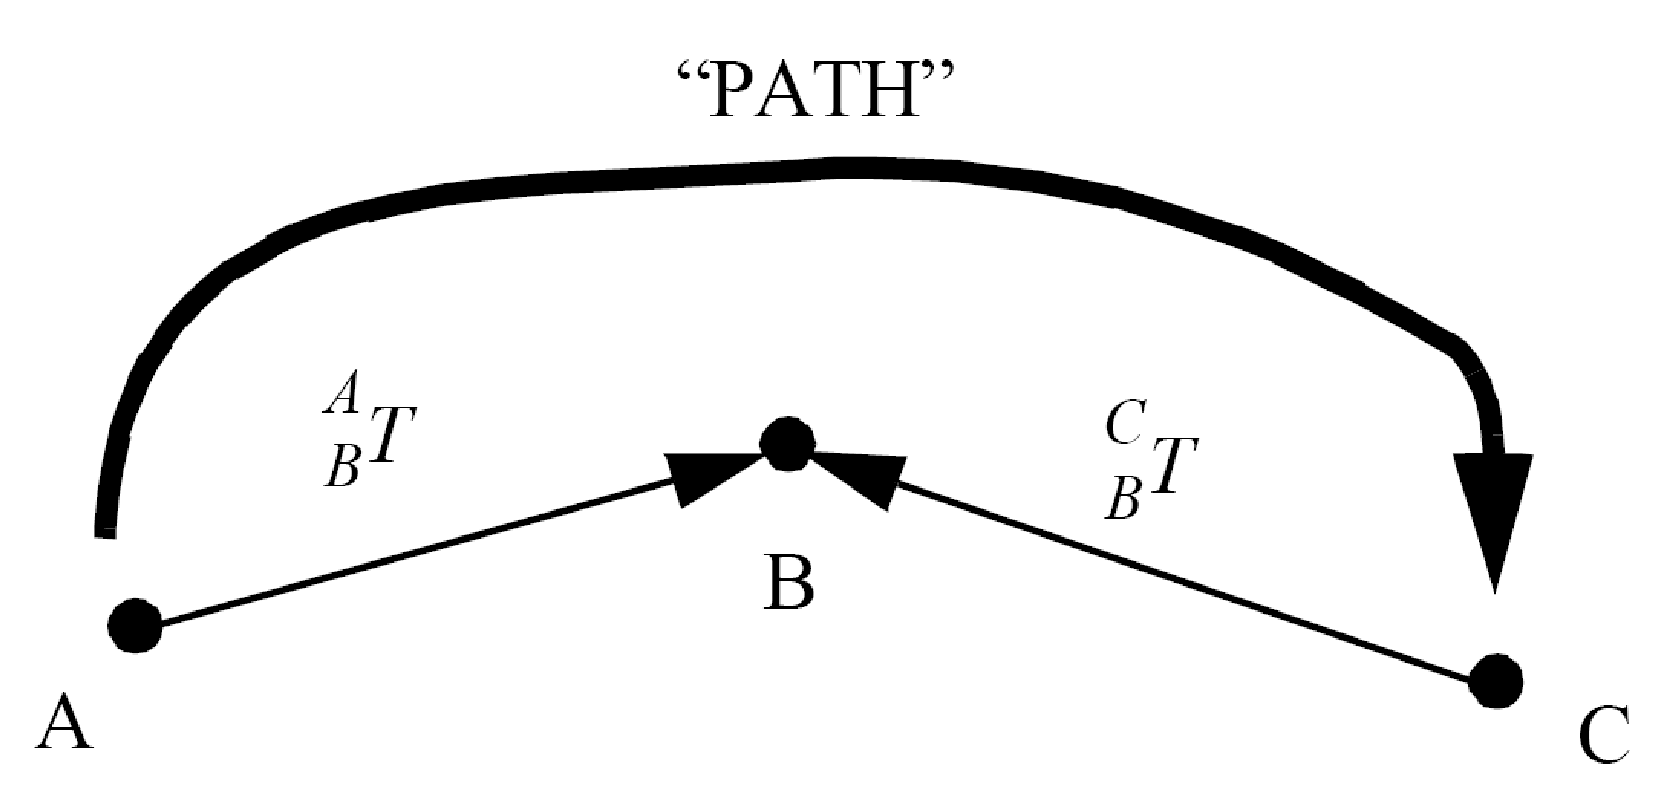
\includegraphics[width=3.5in]{figs02/abgraph.eps}
\caption{A path is  a directed arrow along a chain of transformations.}\label{PATH}
\end{figure}

The transform which shows the PATH in Figure \ref{PATH} is therefore:
\[
^A_CT = \quad ^A_BT(^C_BT)^{-1} = \quad ^A_BT^B_CT
\]
In the first right hand side, $^C_BT$ is inverted because it represents an arrow which goes opposite to the  path.
A closed path in such a graph can be cut at two nodes to form a tranform equation.

%%%%** Figure 9
\begin{figure}[h]\centering
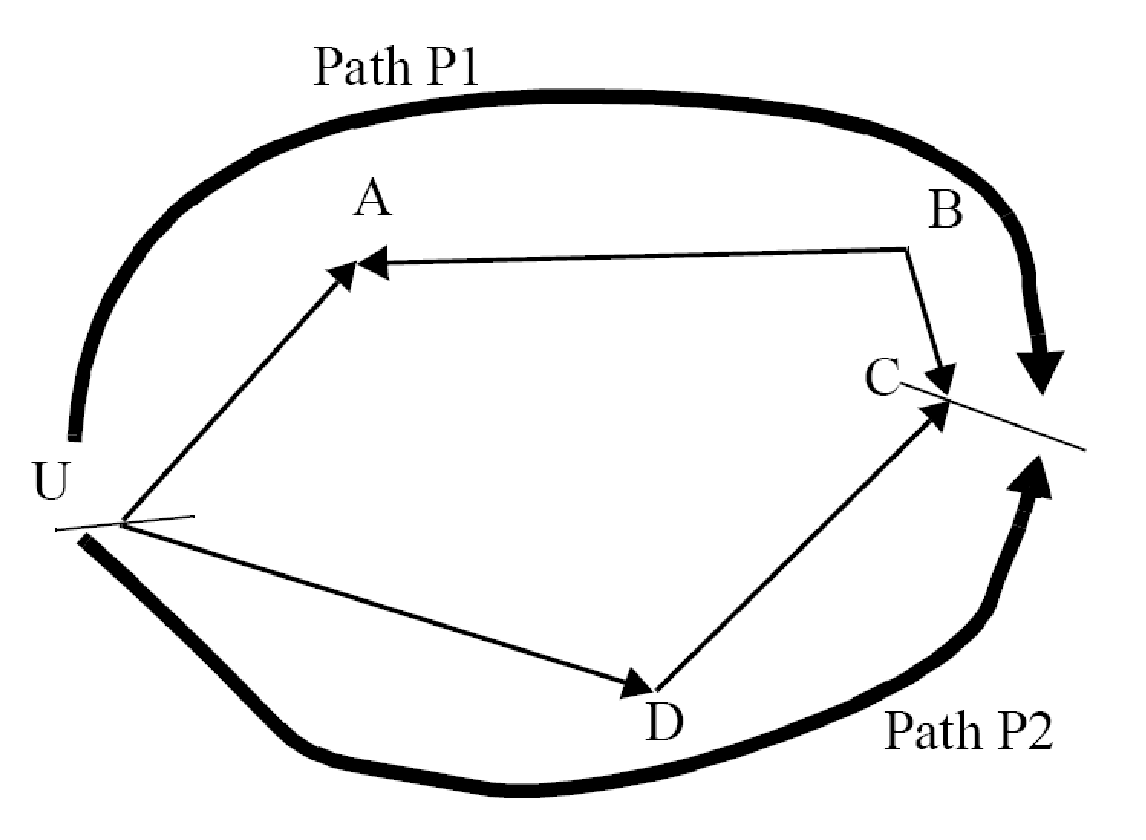
\includegraphics[width=3.5in]{figs02/xformgraph.eps}
\caption{Two paths which start and end at the same point define an equation.}\label{PATHequation}
\end{figure}

In Figure \ref{PATHequation}, the loop is cut at nodes U and C, and the two paths, P1, and P2 represent
the same displacement. Each path corresponds to an equation

\[
\mathrm{P1:} \quad  ^U_CT = ^U_AT \; ^B_AT^{-1} \; ^B_CT
\]
\[
\mathrm{P2:} \quad  ^U_CT = ^U_DT \;^D_CT
\]
And, we can equate the two right hand sides:
\[
^U_AT \;^B_AT^{-1} \; ^B_CT =  ^U_DT \;^D_CT
\]
Furthermore, we can write the equation for a big path going completely
around the loop in, for example, the clockwise direction:
\[
P1(P2)^{-1} = ^U_CT \;^U_CT^{-1} = I_{4\times4}
\]
This is expected since by going completely around the loop we wind up in our original configuration or frame.    Note that when we interpret it as a homogeneous transform, $I_{4\times4}$ corresponds to
\[
\mathrm{Rot}(x,0), \mathrm{Trans}
   \left(  \left [
    \begin{array}{c} 0 \\ 0 \\ 0  \end{array}
    \right ]  \right )
\]



\begin{Example}

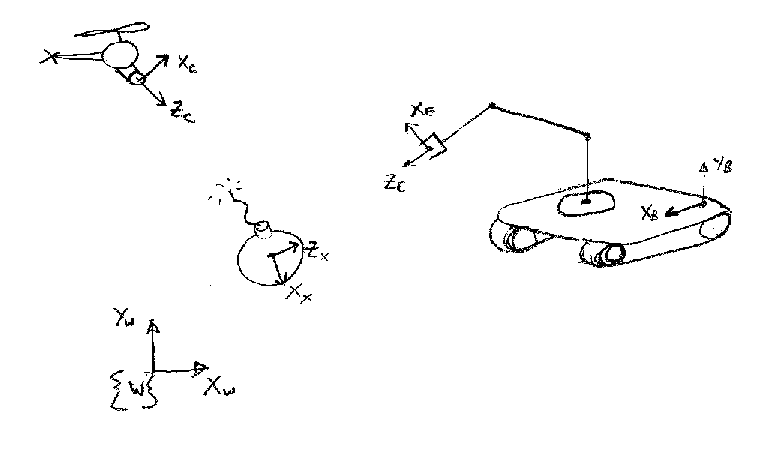
\includegraphics[width=4.75in]{figs02/00487.eps}

A helicopter mounted camera identifies the location and orientation of a bomb.  A bomb disposal robot must understand how to move its arm to pick up the bomb.  The following transforms are known:  ${^C_WT},{^C_XT},{^B_CT},{^B_ET}$

A) Draw the transform graph

B) Solve for ${^X_BT}$

C) Solve for ${^W_ET}$

Answer:

A)

\includegraphics[width=90mm]{figs02/00579.eps}

B)
\[
{^X_BT} = (^C_XT)^{-1}(^B_CT)^{-1}
\]

C)
\[
{^W_ET} = (^C_WT)^{-1}(^B_CT)^{-1}{^B_ET}
\]
\end{Example}


%%%%%%%%%%%%%%%%%%%%%%%%%%%%%%%%%%%%%%%%%%%%%%%%%%%%%%%%%%%%%%%%%%%%%%%%%%%%%%%%%%%%%%%%%%%%%%%%%%%%%%%%%%%%%%%
%
%
\begin{Example}

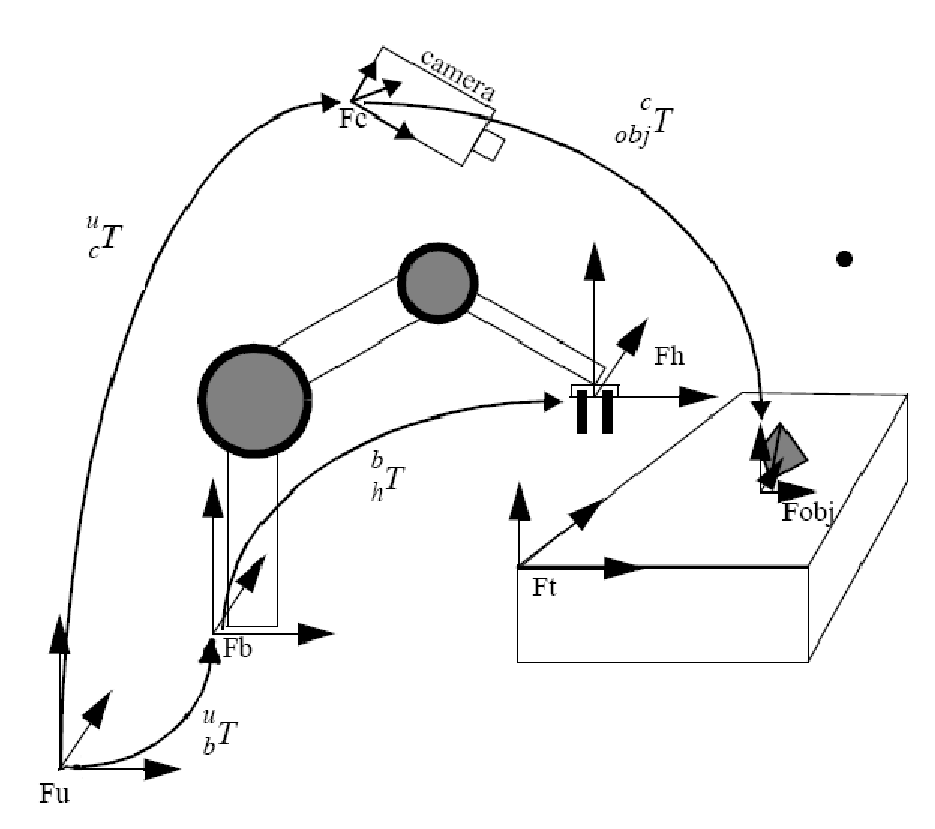
\includegraphics[width=3.5in]{figs02/camtablearmexample.eps}

Let’s consider a factory workstation with a robot arm, worktable, vision
camera, and an object on the table. The known spatial relationships are shown by links in the diagram. Suppose we need to specify the position and orientation of the object so that the robot can pick it up. The robot controller must have the configuration in Fb, the base frame of the robot.

Q1:
What is the configuration of the object in Fb?

A1:
The object can be ``reached" by a path in the transform graph from
Fb through Fu, and Fc, to Fobj. Note that the first link has a direction
opposite to the path we take to the object. The equation of this path
is:
\[
^b_{obj}T = ^u_bT^{-1} \;^u_cT \;^c_{obj}T
\]

Q2:
Suppose we want to find the unknown transforms $^h_tT, ^t_{obj}T$?

A2:
If we add these two transforms to the graph (draw them in yourself),
we now have a loop. We can cut this loop at any two points to make
an equation. Suppose we make these cuts at the hand and at the object.
Now we have
\[
^b_hT^{-1} \;^u_bT^{-1} \;^u_cT \;^c_{obj}T = ^h_tT \;^t_{obj}T
\]
Since the two transforms on the right hand side are unknown, we
cannot solve this without another equation. Now suppose we go out
to the factory floor and measure the location and orientation of the
table. This gives us $^u_tT$. Drawing this link into the transform graph, we see that another loop is formed tangent to the original loop so that we have another equation. One such equation is
\[
^u_bT \;^b_hT \;^h_tT = ^u_tT
\]
We can solve this for one of our unknowns giving:
\[
^h_tT = ^b_hT^{-1} \;^u_bT^{-1} \;^u_tT
\]
Then we substitute to get
\[
 ^b_hT^{-1} \;^u_bT^{-1} \;^u_cT \; ^c_{obj}T = ^b_hT^{-1} \;^u_bT^{-1} \;^u_tT \;^t_{obj}T
\]
\[
^c_{obj}T = ^u_cT^{-1} \;^u_tT \;^t_{obj}T
\]
\end{Example}

\begin{Example}
A revitalized GM plant has installed massive assembly robots.  Such a robot arm must install the engine into a car body.   Frames have been applied to the body and engine as shown below.

\includegraphics[width=5.5in]{figs02/00439.eps}

The following facts are known:

\begin{enumerate}
	\item The engine must be lowered through an intermediate position in order for the transmission to clear the body. This position is $^M_IT$.  Then the engine will be moved into its final position, $^M_CT$.

	\item The car and engine rack are located at known tranforms $^U_CT$, and $^U_RT$ respectively.

	\item GM has finally switched over to the metric system!
\end{enumerate}
Questions:

{\bf Q1)} Give the transform (in numerical form) which specfies the engine position in the rack, $^R_ET$.  Assume that the $z$ position coordinate is zero.

\end{Example}
\begin{ExampleCont}
\subsection*{Solution}

Obtain the rotation matrix by writing the unit vectors of {$E$} expressed in {$R$}, $or$ evaluating Rot($\hat{z},-90^{\circ}$).
\[
{^R_ET} =
\begin{bmatrix}
0 & 1 & 0 & 0.25	\\
-1 & 0 & 0 & 0.25	\\
0 & 0 & 1 & 0		\\
0 & 0 & 0 & 1
\end{bmatrix}
\]

{\bf Q2)} You need to program the robot to take the engine from the rack and put it in the intermediate position.  Solve for the transform which represents the intermediate engine position and orientation relative the engine rack, $^R_IT$ in terms of the known transforms above.

\subsection*{Solution}
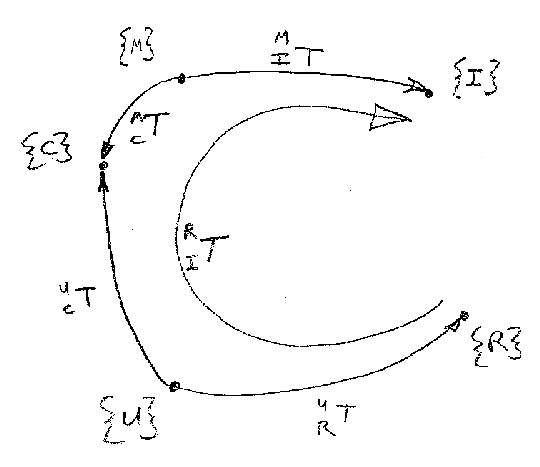
\includegraphics[width=3.5in]{figs02/00440.eps}

going around the transform graph in the direction shown, we have:
\[
{^R_IT} \quad = \quad {^U_RT^{-1}} \quad {^U_CT} \quad {^M_CT^{-1}} \quad {^M_IT}
\]
\end{ExampleCont}



\begin{Example}
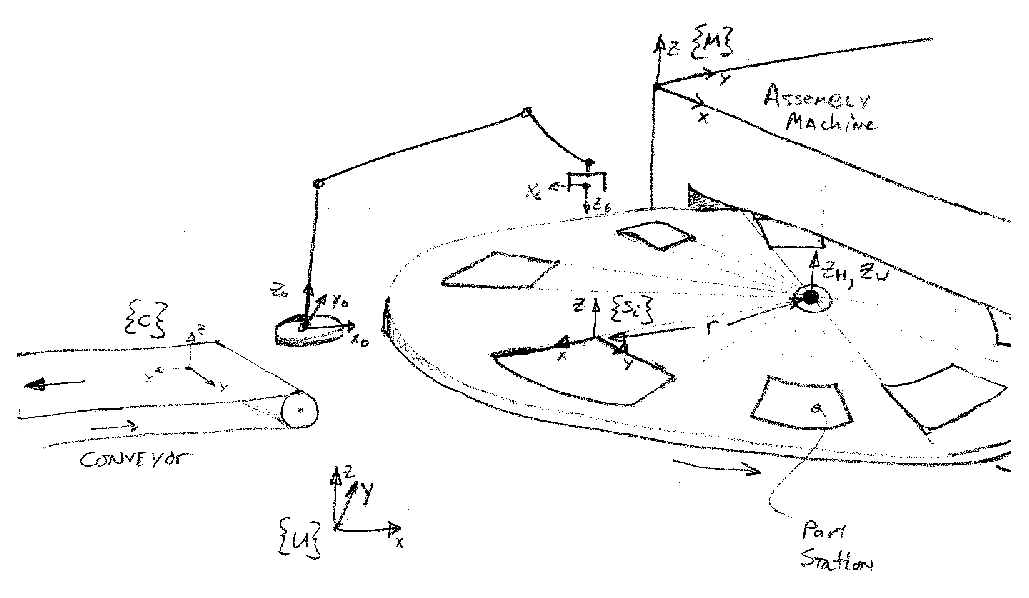
\includegraphics[width=6.4in]{figs02/00080.eps}


\subsection*{Pizza Problem}
Completed assemblies (pizzas?) come out of a machine on a large rotary
table. Pizzas are numbered $i=\{1,2,3 ...}$.  You must program a robot arm to pick up the pizzas and transfer
them to a conveyor.


Use the following facts:

\begin{itemize}
	\item The part stations are spaced every $36^\circ$ on the wheel.

	\item The robot base frame is \{$0$\} and the end effector frame
is \{$6$\}.

	\item The origin of frame $H$ is located at the wheel hub:
\[
^U_HT =  \left[ \begin{array}{cccc}
1 & 0 & 0 & 10  \\
0 & 1 & 0 & 10 \\
0 & 0 & 1 & 2 \\
0 & 0 & 0 & 1
\end{array}  \right]
\]
	\item The $i^{th}$ part station has frame \{$S_i$\} located at its corner.
	The distance from the origin of \{$H$\} to the origin of \{$S_i$\}
	is $r=5$.
	\item Another frame \{$W$\} has the same origin as \{$H$\}, but $X_W$
always points to the origin of \{$S_1$\}.

	\item The front panel of the machine is at
\[
^U_MT =  \left[ \begin{array}{cccc}
0  & 1 & 0 & 10  \\
-1 & 0  &0  & 16 \\
0 & 0 & 1 & 4 \\
0 & 0 & 0 & 1
\end{array}  \right]
\]

	\item $\Theta_W(t)$ describes the rotation of the wheel.  $\Theta_W$ is
the angle from $X_H$ to $X_W$.

\end{itemize}



\end{Example}


\begin{ExampleCont}
{\bf Q1:}
If $t$ is in seconds, $\Theta_W(t) =  \frac{\pi}{15}t$ rad or
$\Theta_W(t) =  12t$ degrees, what is $^U_ST(i,t)$, i.e. what is the
transform from frame $U$ to frame $S_i$ (multiply out your answer).

\subsection*{Solution:}

\[
{^U_{Si}T} \quad= \quad {^U_HT} \quad {^H_WT} \quad {^W_{Si}T}
\]
From the facts,
\[
{^H_WT} = \mathrm{Rot}(\hat{z}, 12t^{\circ})
\]
\[
{^W_{Si}T} =  \mathrm{Rot}(\hat{z}, (36(i-1))^{\circ} )
\]
\[
{^U_{H}T} \quad= \quad
\begin{bmatrix}
1 & 0 & 0 & 10	\\
0 & 1 & 0 & 10 	\\
0 & 0 & 1 &  2  \\
0 & 0 & 0 &  1
\end{bmatrix}
\]
Since the last two are both about the $\hat{z}$ axis, we can add their displacements to simplify.  Let
\[
\alpha = (12t + 36(i-1))^{\circ}
\]
Then
\[
{^U_{Si}T} \quad= \quad
\begin{bmatrix}
1 & 0 & 0 & 10	\\
0 & 1 & 0 & 10 	\\
0 & 0 & 1 &  2  \\
0 & 0 & 0 &  1
\end{bmatrix}
\mathrm{Rot}(\hat{z}, \alpha)
\]
\[
{^U_{Si}T} \quad= \quad
\begin{bmatrix}
1 & 0 & 0 & 10	\\
0 & 1 & 0 & 10 	\\
0 & 0 & 1 &  2  \\
0 & 0 & 0 &  1
\end{bmatrix}
\begin{bmatrix}
c\alpha & -s\alpha & 0 & 0	\\
s\alpha &  c\alpha & 0 & 0 	\\
0 & 0 & 1 &  0  \\
0 & 0 & 0 &  1
\end{bmatrix}
\]
\[
{^U_{Si}T} \quad= \quad
\begin{bmatrix}
c\alpha & -s\alpha & 0 & 10	\\
s\alpha &  c\alpha & 0 & 10 	\\
0 & 0 & 1 &  2  \\
0 & 0 & 0 &  1
\end{bmatrix}
\]

{\bf Q2:}
If $^U_0T, \quad ^0_6T, \quad ^U_ST(i,t)$ are known, draw a transform graph, and solve
for $^6_ST(i,t)$.

\subsection*{Solution:}

Transform Graph:

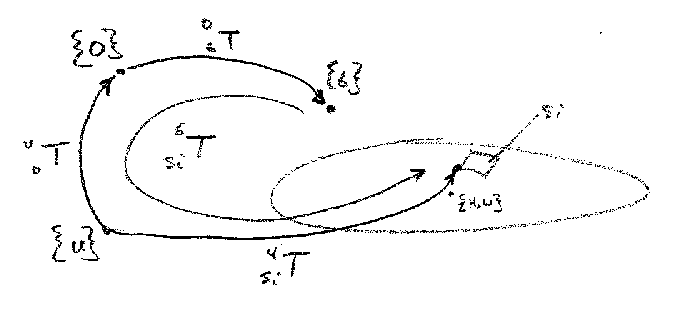
\includegraphics[width=4.3in]{figs02/00443.eps}

\[
{^6_{Si}T} \quad = \quad {^0_6T}^{-1} \quad {^U_0T}^{-1}  \quad {^U_{Si}T}
\]

\end{ExampleCont}















%
%
%
%
% \section{Quaternions}
%
% (to be written)

%  Table row height
\renewcommand\arraystretch{0.2}% Vertical Row size, 1.0 is for standard spacing)


%%%%** Section 11
\section{Exponential Coordinates}

The following elegant notation and derivation is based closely on {\bf Murray, Li, and Sastry, ``A Mathematical Introduction to Robotic Manipulation", CRC Press, 1994.}

%%%%** Section 11.1
\subsection{Rotation}\label{Rotation}

Consider the velocity of a point $q$ which is rotating about an axiz $\omega$.  We assume that
$|\omega|=1$ and its direction is the axis of rotation. We can write the velocity of the point as
\[
\dot{q}(t)=\omega \times q(t)
\]

Recall that the vector cross product ($\times$) can be represented as the product of a special
skew-symmetric matrix,
\[
\hat{\omega} = \left[
\begin{array}{ccc}
0               &       -\omega_3       &       \omega_2      \\
\omega_3        &       0               &       -\omega_1     \\
-\omega_2       &       \omega_1        &       0             \\
\end{array}
\right]
\]
with the vector, i.e.
\[
\omega \times q = \hat{\omega} q
\]
So we have
\[
\dot{q}(t)=\hat{\omega} q(t)
\]
This is a first order differential equation with the solution
\[
q(t) = e^{\hat{\omega}t}q(0)
\]

Now we need to understand what it means to take the exponential of a matrix!
Using the Taylor series expansion, we have:
\[
\exp(A) = I + A + \frac{A^2}{2!} + \frac{A^3}{3!} + ...
\]
We are interested in the special case of
\[
A = \hat{\omega}t
\]
where $\hat{\omega}$ is the matrix defined as above and $t$ is a scalar (time).
One interpretation is that we can parameterize any rotation by the amount of time
it takes at unit velocity ($|\omega|=1$). Thus we can also write
\[
R(\omega,\Theta) = e^{\hat{\omega}\Theta}
\]
where
\[
\Theta = |\omega|t
\]

To evaluate the matrix exponential, we sort the series out into odd and even terms (and perform
a few other tricks) to get:
\[
e^{\hat{\omega}\Theta} =
    I
 +
    \left(
       \Theta - \frac{\Theta^3}{3!} + \frac{\Theta^5}{5!} + \dots
    \right)\hat{\omega}
 +
    \left(
       \frac{\Theta^2}{2!} + \frac{\Theta^4}{4!} + \frac{\Theta^6}{6!} + \dots
    \right)\hat{\omega}^2
\]
Which simplifies to
\[
e^{\hat{\omega}\Theta} = I + \hat{\omega} \sin \Theta + \hat{\omega}^2(1-\cos\Theta)
\]
So $e^{\hat{\omega}\theta}$ is the rotation matrix which expresses rotation by $\theta$ about
axis $\omega$.

This can also be inverted (See Murray, Li, Sastry, equations (2.17) and (2.18),
or Craig, equations (2.81) and (2.82)):
\begin{equation}\label{thetainverse}
\theta = cos^{-1} \left(
        \frac {r_{11} + r_{22} + r_{33} -1}
              {2}
        \right)
\end{equation}
\begin{equation}\label{omegainverse}
\omega = \frac{1}{2sin\theta} \left[
        \begin{array}{c}
        r_{32}-r_{23}   \\
        r_{13}-r_{31}   \\
        r_{21}-r_{12}   \\
        \end{array}
        \right]
\end{equation}




%%%%** Section 11.2
\subsection{Translation and Rotation}
Consider a point, $p(t)$ whos position is a function of time.  Assume that the point is displaced due to
rotation about an axis, $\omega$, separate from the point.  We assume that $|\omega|=1$ and that $q$ is
a point {\bf off} the axis. The velocity of the point is then
\[
\dot{p}(t) = \omega \times (p(t) - q)
\]
or
\[
\dot{p}(t) = \omega \times p(t) - \omega \times q
\]
Using $\hat{\omega}$ as defined above, if we define
\[
\hat{\xi} = \left[
\begin{array}{cc}
\hat{\omega}   &       -\omega\times q \\
0       &       0       \\
\end{array}
\right]
\]
and we express $p(t)$ and its derivative in homogeneous coordinates,
\[
\dot{p} =  \left[
\begin{array}{cc}
\hat{\omega}   &       -\omega\times q \\
0       &       0       \\
\end{array}
\right]
\left[
\begin{array}{c}
p\\
1\\
\end{array}\right]
\]
In this special case (of rotation about an axis remote from $\omega$) the velocity
of the point $p$ is $-\omega\times q$.  More generally, we can write
\[
\dot{p} =  \left[
\begin{array}{cc}
\hat{\omega}   &       v \\
0       &       0       \\
\end{array}
\right]
\left[
\begin{array}{c}
p\\
1\\
\end{array}\right]
\]

More compactly:
\[
\dot{p} = \hat{\xi}p
\]

the matrix $\hat{\xi}$ is refered to as a {\it twist}.

This is a first order differential equation which has the solution:
\[
p(t) = e^{\hat{\xi}t}p(0).
\]
Recall that $\hat{\xi}$ doesn't have as simple a form as $\hat{\omega}$ and so it is
not as easy to get an expression for $e^{\hat{\xi}t}$.
It can be shown that (see Murray, Li, and Sastry, Proposition 2.8) that for a displacement which
consists of rotation $\hat{\omega}\Theta$ and displacement $v\theta$
\begin{equation}\label{matrixexp}
e^{\hat{\xi}\theta} =
\left[
  \begin{array}{cc}
  e^{\hat{\omega}\theta}   & (I-e^{\hat{\omega}\theta})(\omega\times v) + \omega\omega^Tv\theta          \\
  0                        &       1                               \\
  \end{array}
\right]
\end{equation}

As used here, $\theta$ is a general motion parameter and need not be an angle.
The interpretation of $e^{\hat{\xi}\theta}$ is a description of a physical manipulation
i.e.
\[
^Ap(\theta) = {e^{\hat{\xi}\theta}}    {^Ap(0)}
\]
Note that both $^Ap(\theta)$ and $^Ap(0)$ are represented in the same frame, $A$, which
should also be the same as that used for $\omega$ and $v$.

To represent a known physical displacement as a twist, we first must know the 4x4 homogeneous
transform defining the displacement, $^A_BT$ which the authors call $g_{ab}$.
Given $g_{ab}$, we solve for the ``twist coordinates", $\omega, \theta, v$ equating
(\ref{matrixexp}) with the known $g$:
\[
g = \left [
        \begin{array}{cc}
        R               &               P       \\
        0               &               1       \\
        \end{array}
\right]
=
\left[
        \begin{array}{cc}
  e^{\hat{\omega}\theta}   & (I-e^{\hat{\omega}\theta})(\omega\times v) + \omega\omega^Tv\theta          \\
  0                        &       1                               \\
        \end{array}
\right]
\]
for
\[
R = e^{\hat{\omega}\theta}
\]
we had equation (\ref{thetainverse} and (\ref{omegainverse}) to find $\theta$ and $\omega$.
To get $v$, we have
\[
P = (I-e^{\hat{\omega}\theta})(\omega\times v) + \omega\omega^Tv\theta
\]
which we can solve by hand calculation or Mathematica for $v$.  There are some useful special
cases. For example for a simple axis such as
\[
\omega = \left [
        \begin{array}{c}
        0\\0\\1\\
        \end{array}
        \right ]
\]
the equation to solve is
\[
\left[
        \begin{array}{ccc}
        s\theta &       c\theta -1      &       0\\
        1-c\theta   &   s\theta         &       0\\
        0              &        0       &   \theta\\
        \end{array}
\right]
v = P
\]
In the special case of revolute motion about the axis $\omega$, $v$ is only due to the
rotation and so it is known:
\[
v = -\omega \times q
\]

%%%%** Section 11.3
\subsection{Groups}
Murray, Li, and Sastry take some pains to relate these kinematic ideas to group theory.
The basic properties of a group are
\begin{itemize}
        \item It consists of a set of objects, $G$ and a binary operation, $\times$.
        \item It is ``closed" in the sense that if any two objects in the
        group are applied to the binary operation, the result is another member
        of the group.
        \item There exists an ``identity element", $i$, which is a member of the
        group such that $g \times i = g$.
        \item For every element of the group, $g$, there is a unique inverse, also a
        an element of the group, $g^{-1}$
         such that $g\times g^{-1} = i$.
        \item The operation is associative:  $(g_1\times g_2)\times g_3= g_1 \times (g_2\times g_3)$.
\end{itemize}
For example, you can verify that these five properties hold for the set of orthonormal 3x3 rotation matrices together with
the operation of matrix multiplication, and so they must form a group.

Murray, Li, and Sastry named four groups which are relevant to robotic manipulation:
\begin{description}
        \item[$se(3)$] the group of 4x4 skew symmetric matrices (twists)
        \item[$so(3)$] the group of 3x3 skew symmetric matrices ($\hat{\omega}$).
        \item[$SE(3)$] the group of 4x4 homogeneous transforms
        \item[$SO(3)$] the group of 3x3 orthonormal rotation matrices
\end{description}


%%%%** Section 12
\section{Summary of Notation}

% Summary of Notation for Chapter  02

  % coordinate transforms & rigid body motions
 %  Robotics Text  by Jacob Rosen and Blake Hannaford
% (c) 2007  Jacob Rosen and Blake Hannaford
%

\chapter{Forward Kinematics}





\section{Problem Statement and Learning Objectives}
% Problem Statement and Learning Objectives for Chapter 03
\paragraph{Problem Statement}
 This chapter addresses the problem of computing the position and orientation of an end effector, knowing the geometry of the manipulator and the position values of each joint.  Joints may be rotary in which case the joint value is an angle, or prismatic, in which case the joint value is a displacement. We seek a general way to represent any serial manipulator. 

\paragraph{Learning Objectives}
 
After completing this chapter, the student will be able to derive the forward kinematic model of a serial manipulator.  Specifically to
\begin{itemize} 
  \item Identify the link and joint geometry from a picture or engineering drawing of a serial mechanism containing rotary and prismatic joints.
  \item Be able to assign a coordinate system to each link in a standardized manner. 
  \item Be able to derive Denavit-Hartenberg parameters for each link
  \item Be able to form the 4x4 homogeneous transform for each link based on the DH parameters and be able to multiply these link matrices together to get a symbolic expression for the forward kinematic equations in the form of a 4x4 homogenous transform matrix. 
\end{itemize}
The result is a computation of the position and orientation of the end effector knowing the geometric dimensions  of each link and the position of each joint in the mechanism.  






\section{Serial Mechanisms}

\subsection{Links and Joints}

\subsubsection{Links}
In this chapter we study the spatial relationships (transforms) between the links of a robot arm. First we define an {\it axis of motion} as
\begin{quotation}
A line in 3-space which contains points which are not moved by a particular rotation (a {\it rotary} axis), or which contains a direction describing linear motion (a {\it translation} axis).
\end{quotation}

We will define a {\it link} as
\begin{quotation}
A spatial relation, enforced by a rigid object, between two axes of motion.
\end{quotation}
In a typical robot arm, the links are rigid structural elements (most often of metal) which hold at each end the bearings for a joint.   Their rigidity enforces a constant spatial relationship between axes of motion at the {\it proximal} (closer to the base) and {\it distal} (closer to the end effector) ends.

\begin{figure}\centering
\includegraphics[width=2.75in]{figs03/00718.eps}
\caption{"Link", a rigid body which enforces a fixed spatial relationship between two axes of motion.}\label{LINK}
\end{figure}

\subsubsection{Joints}

Joints connect the links in a serial kinematic chain.  We define a joint as
\begin{quotation}
A structural element which allows relative motion between two bodies in only one degree of freedom.  Such motion is constrained to translational motion along a line or rotation around a line.
\end{quotation}

We have two classes of joints, {\it rotational} and {\it translational}, also known as {\it prismatic}\footnote
{Think of a prism sliding inside a hole shaped to match its profile.  It can slide in and out, but not rotate.}.   Combining the definitions of link and joint, we see that each axis of motion is fixed in the two links adjoining the joint.   The degree of translation or rotation (the single motion freedom of the joint) is called the joint variable.    Since the joint constrains relative motion of the two links to a single degree of freedom, the joint variable is sufficient to describe the spatial relationship between them.


\begin{figure}\centering
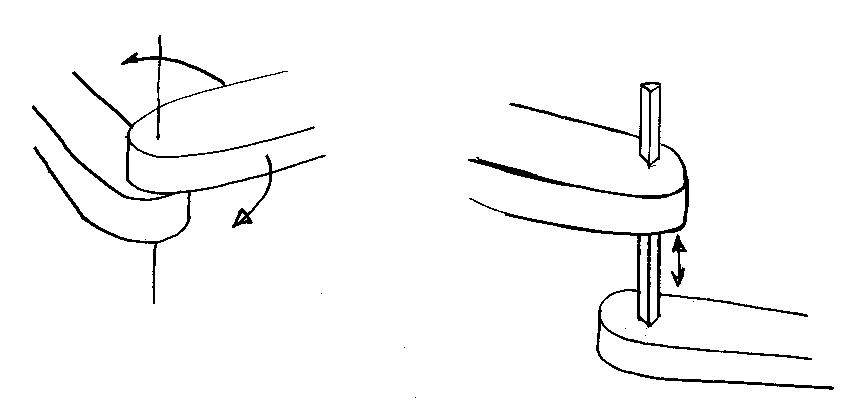
\includegraphics[width=3.5in]{figs03/00341.eps}
\caption{Two types of joints, rotational and translational/prismatic.}\label{RotationalTranslationalJoints}
\end{figure}


A series of such links bridging adjacent axes is an open kinematic chain (also known as a robot arm!).
The {\it forward kinematics} problem is to find the position and orientation of the last link in the chain (i.e. the robot hand) knowing only the robot's geometry and the angles or displacements of the joints. To make our method general, we will assume that there can be any amount of twist, displacement, and offset between the ends of each link. This make the problem difficult unless we employ a systematic approach.  We will use the approach invented by Denavit and Hartenberg in which we will construct a virtual kinematic chain which is equivalent to the original robot but is easier to analyze.  The virtual kinematic chain in the ``DH" method consists of the joint axes and their {\it common normals}.   The common normal between two lines or axes is a unique\footnote{Not always unique but see below.} line which is perpendicular to both axes.




\subsection{Modeling Links and Joints}


\begin{figure}
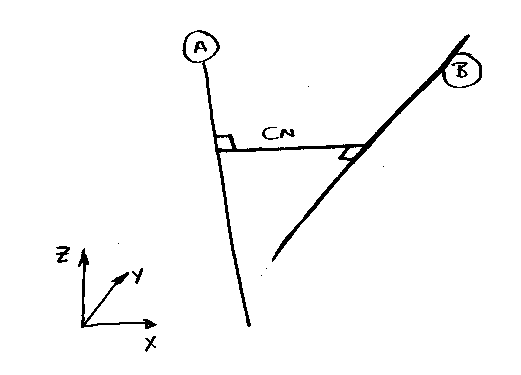
\includegraphics[width=3.5in]{figs03/00337.eps}
\caption{The Common Normal (CN) is the shortest line which intersects two given lines.  It intersects  lines {\bf A} and {\bf B}  at a right angle.}\label{CommonNormals}
\end{figure}


\begin{figure}
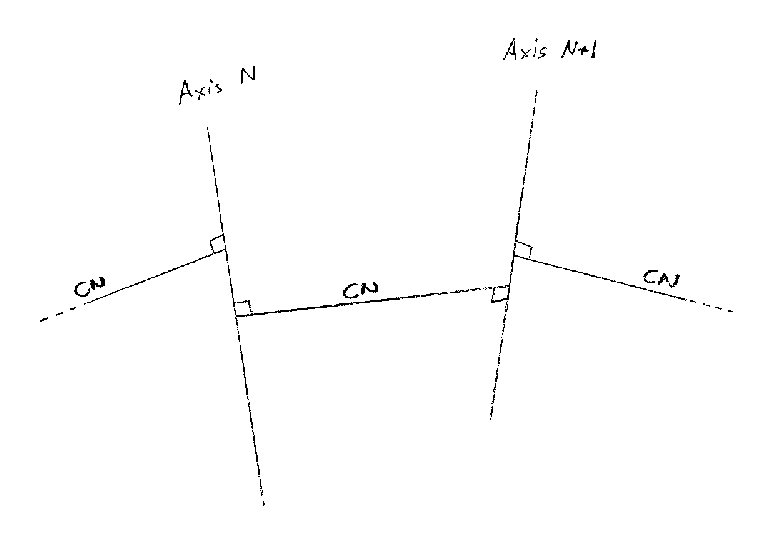
\includegraphics[width=3.5in]{figs03/00339.eps}
\caption{Virtual Links between axes are formed by the Common Normals.}\label{VirtualLinksCN}
\end{figure}

\subsubsection{Assignment of Frames to Links}
We will define a series of frames along the virtual kinematic chain and identify the key rotations and translations which define their relationships.


\paragraph{Common Normal}

The CN will be our virtual link between two axes in space.   It is worth noting that the CN might be completely outside the physical structure of the robot.  However our virtual manipulator constructed using CNs will be an exact representation of the kinematics of the real one.   It turns out that we can identify the CN of each link rather informally.  We do not need to write the equation for each CN line segment but it will be more important to identify the two end points.

There will be a CN for each pair of joint axes (Figure \ref{VirtualLinksCN}).  If the two joint axes are parallel, there are an infinite number of CNs so we just choose one arbitrarily.  If the two axes intersect, then the CN has zero length but it still has a direction which is the cross product

\begin{equation}
CN = \mathrm{Axis}_N \otimes \mathrm{Axis}_{N+1}
\end{equation}


%%%%%%%%%%%%%%%%%%%%%%%%%%%%%%%%%%%%%%%%%%%%%%%%%%%%%%%%%%%%%%%%%%%%%%%%%%%%%%%%%%%%%%%%%%%%%%%%%%%%%%%%%%
\begin{ExampleSmall}
Find the Common Normal between the following lines:
\[
x=0, y=0
\]
and
\[
z=1, x=1
\]

The common normal is also the shortest line segment which intersects both lines.   The first line is a vertical along the $z$ axis.  The second goes in the $y$ direction through the point $[1 \quad 0\quad 1]^T$.    The shortest line segment connecting these two lines is the line segement between $[0\quad 0\quad 1]^T$ and $[1\quad 0\quad 1]^T$ which is the line
\[
z=1, y=0
\]

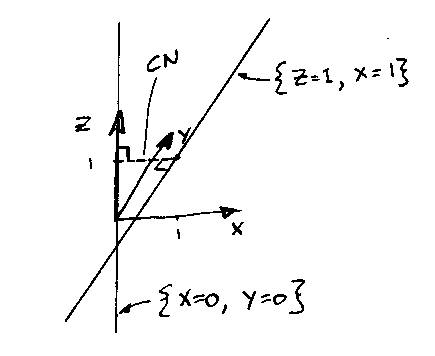
\includegraphics[width=2.5in]{figs03/00338.eps}

\end{ExampleSmall}



\subsection{Fixing Frames to Links}

Once we identify common normals between the manipulator axes, we are ready to locate a frame, rigidly attached to each link.  Although conceptually these could be anywhere, our convention will locate them on the joint axes.  We will  first choose the location of the origin, and then the directions for two axes.   The third axis follows by the right hand rule.


The origin of the link frame will be at the point where Axis $N$ intersects the CN to Axis $N+1$.  Let's call this point $A_N$.    The $X_N$ axis will point along the CN toward its intersection with the following axis.  Let's call the other end of the CN $B_N$.   $Z_N$ will point along the joint axis.  There are two ways that $Z_N$ can point along $Z_N$.    For rotary joints, we will require that we choose the direction of $Z_N$ so that positive rotation of the joint is consistent with the right-hand-rule about $Z_N$.  The points $A_N$ and $B_N$ are shown in Figure \ref{VirtualLinkswFrames}.

Now that $X_N$ and $Z_N$ are fixed, we choose $Y_N$ simply by
\[
Y_N = Z_N \otimes X_N
\]

\begin{figure}[p]
\centering
A)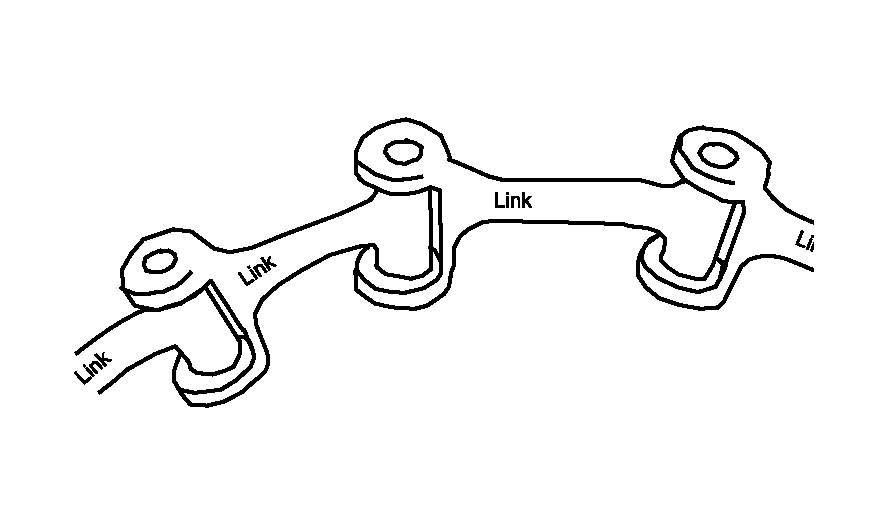
\includegraphics[width=5.0in]{figs03/linkdiag_plain.eps}\\
B)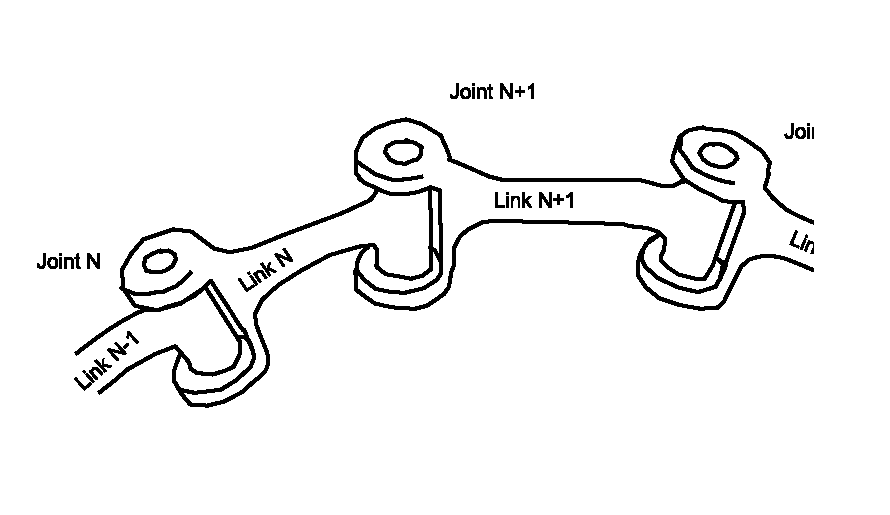
\includegraphics[width=5.0in]{figs03/linkdiag_idlinksjoints.eps}\\
C)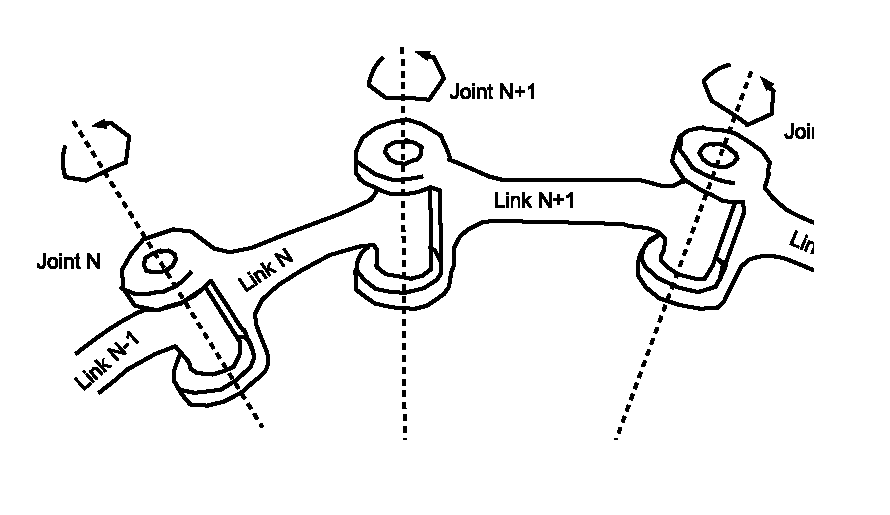
\includegraphics[width=5.0in]{figs03/linkdiag_idaxestypes.eps}
\caption{Summary of steps for analyzing the DH parameters of a serial chain.}\label{DHStepsSummary}
\end{figure}
\begin{figure}[p]
\centering
D)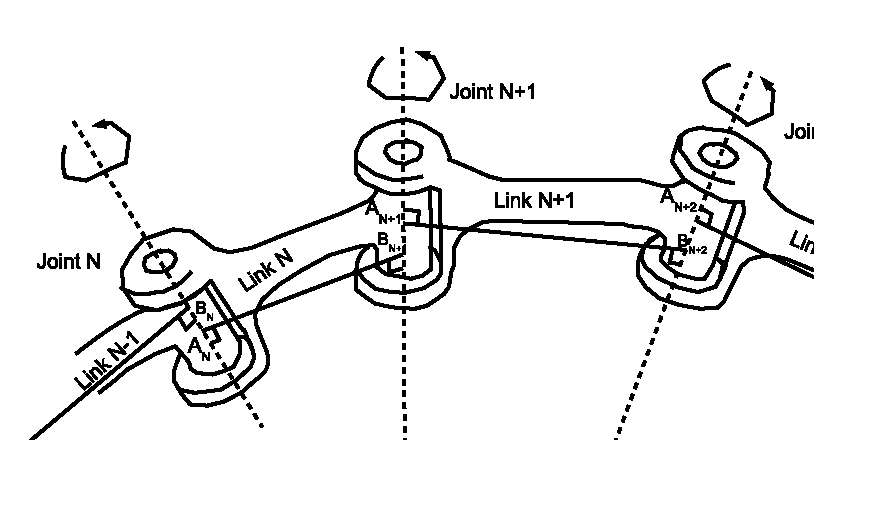
\includegraphics[width=5.0in]{figs03/linkdiag_commonnorms.eps}\\
E)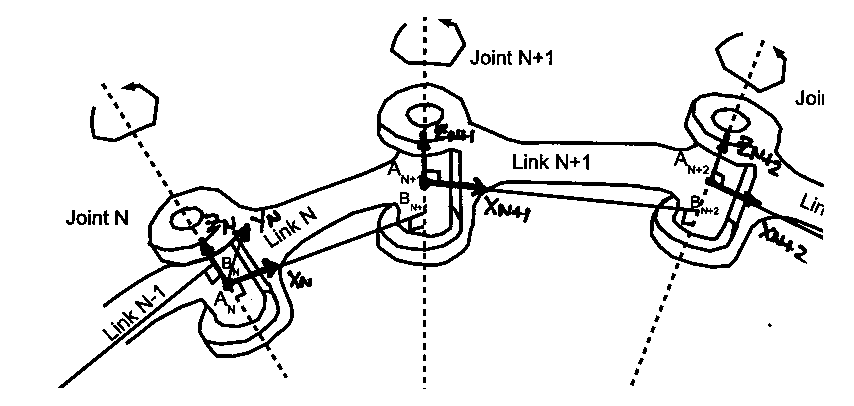
\includegraphics[width=5.0in]{figs03/00336.eps}\\
\caption{Figure \ref{DHStepsSummary} cont.}\label{DHStepsSummary2}
\end{figure}


\clearpage        %  clear floating figures so they appear at next full page



\section{Summary of Link Frame Assignment Methodology}\label{Steps}
We will use the following procedure identify and assign link frames:
\begin{enumerate}
	\item  Understand the geometry and dimensions of the mechanism. Figure \ref{DHStepsSummary}A shows two links (plus parts of two others) of a mechanism we will analyze.


\item Number the links and joints.   The Base of the mechanism is, by convention link 0, and the first joint from the base is numbered joint 1.   In Figure \ref{DHStepsSummary}B we have applied numbers to the links (somewhere in the middle of the chain).




\item  Identify the axes of motion and the directions which you will call positive motion (Figure \ref{DHStepsSummary}C).




\item Draw common normals (CNs) and find their intersections with joint axes.  Define two points on each link:

$A_N$  the intersection of Axis $N$ with the CN to Axis $N+1$.

$B_N$  the intersection of Axis $N$ with the CN to Axis $N-1$.

(Figure \ref{DHStepsSummary}D)


	\item Assign a frame to each link as follows:

The origin of Frame $N$ is $A_N$.

$Z_N$ points along Axis $N$.

$X_N$ points along the CN to $B_{N+1}$

$Y_N$ completes a right handed coordinate system.

(Figure \ref{DHStepsSummary}E)


\end{enumerate}

\vspace{0.25in}


Q:  What if it appears that there is no common normal because the axes intersect?

A: Create a common normal vector with direction but zero length (draw it like a unit vector).
Choose $X_N$ to be normal to $Z_N$ and $Z_{N+1}$.

Q: What if $Z_N$ and $Z_{N+1}$ are parallel and there is no {\it unique} CN?

A: Just choose one of the set of CNs arbitrarily.  Typically you can simplify subsequent analysis by choosing a CN which intersects $B_N$.

Q: What if $Z_N$ and $Z_{N+1}$ are co-linear?

A: Then choose any zero-length vector perpendicular to both of the axes.




%%%%%%%%%%%%%%%%%%%%%%%%%%%%%%%%%%%%%%%%%%%%%%%%%%%%%%%%%%%%%%%%%%%%%%%%
%
%       Example:  Link Frame Assignments, 3 DOF
%
\begin{Example}\label{FKex1}
Assign link frames to the arm shown below.   This arm has two degrees of freedom, but we will define a third frame at the end effector as though the end effector had a degree of freedom attached. The thickness (width) of the arm links is 20cm.


First, we identify the links and joints and number them, starting with link zero and with joint 1 between link zero and link one (blue).
%
% 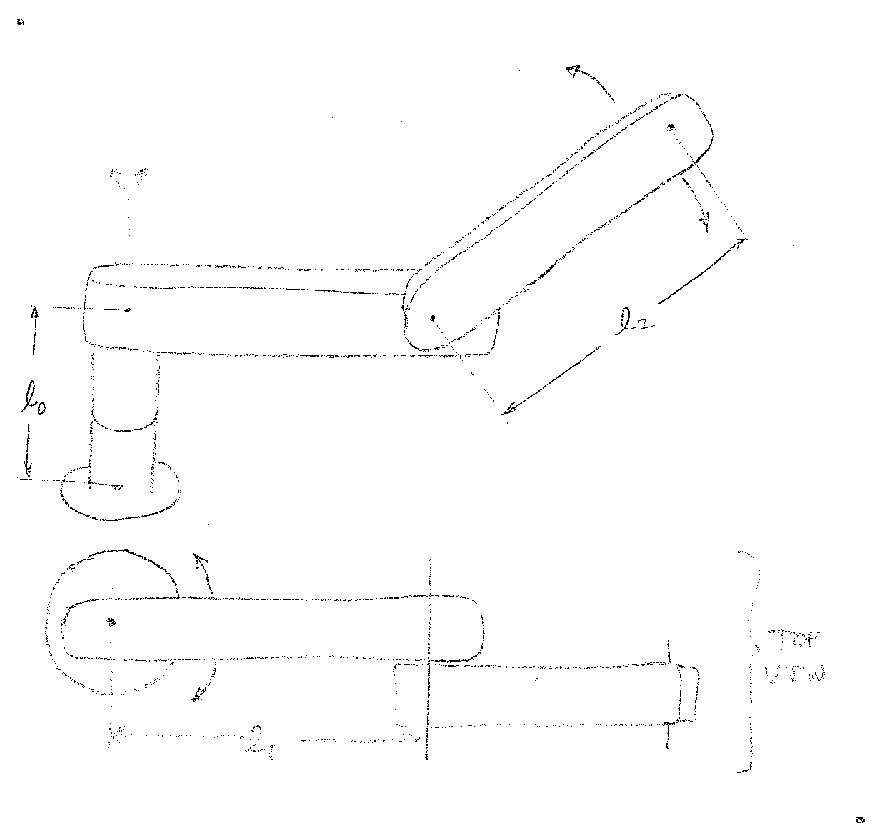
\includegraphics[width=3.25in]{figs03/00408.eps}
%
% \begin{tabular}{cc}
% 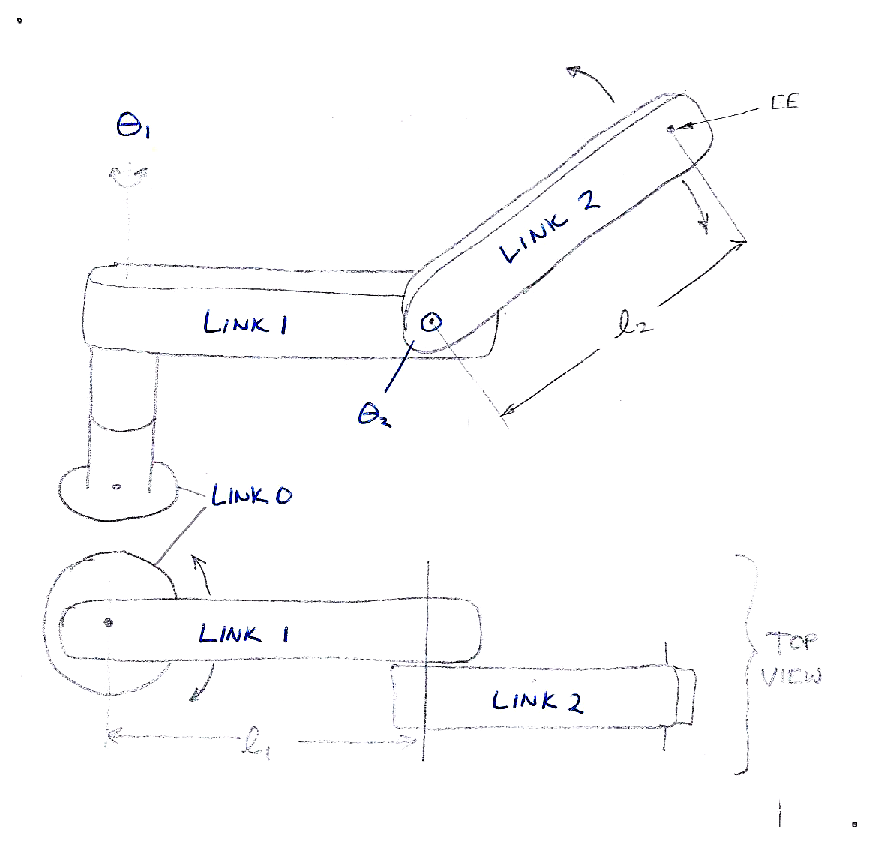
\includegraphics[width=3.25in]{figs03/00409.eps}
% &
% 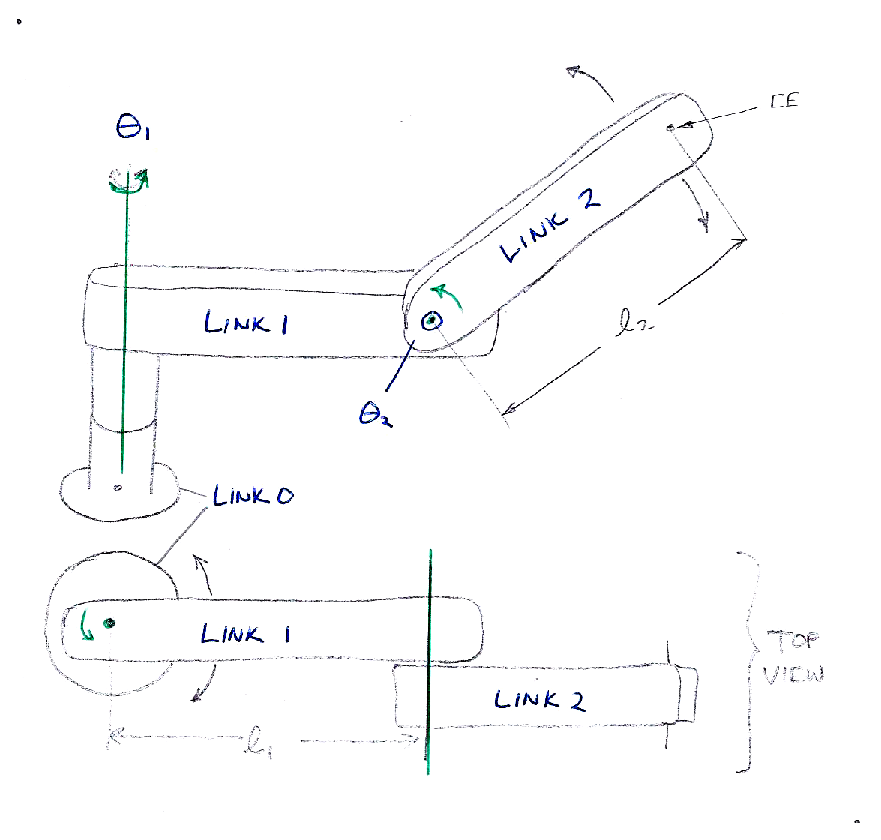
\includegraphics[width=3.25in]{figs03/00410.eps}
% \end{tabular}
% \end{Example}
%
% \begin{ExampleCont}
% \begin{tabular}{cc}
% 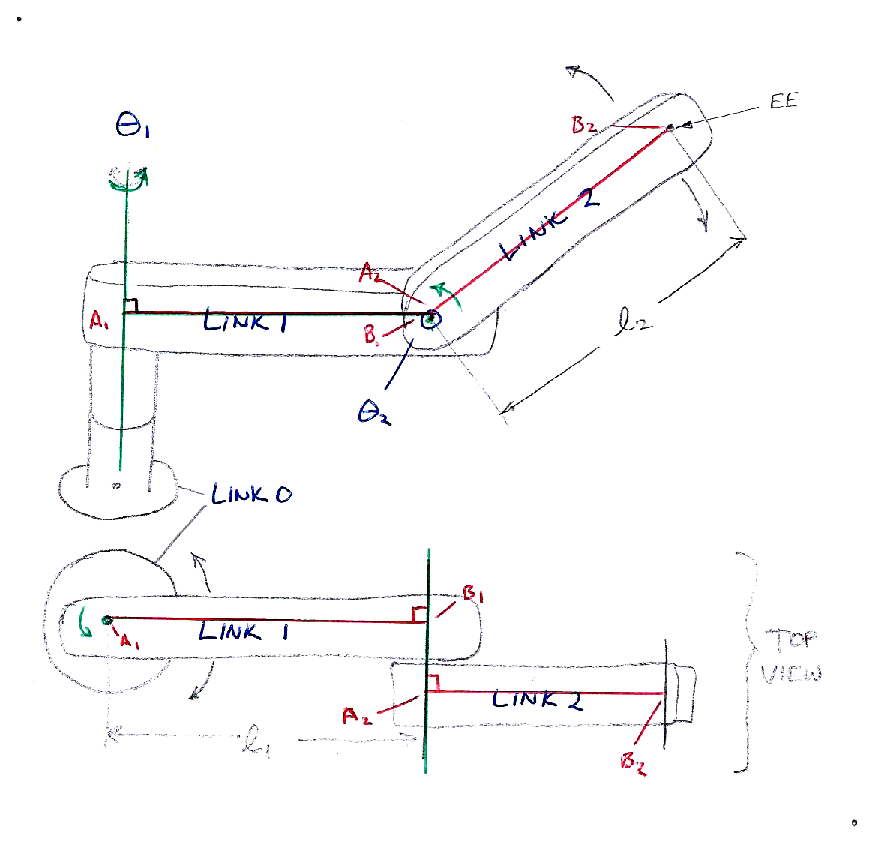
\includegraphics[width=3.25in]{figs03/00411.eps}
% &
% 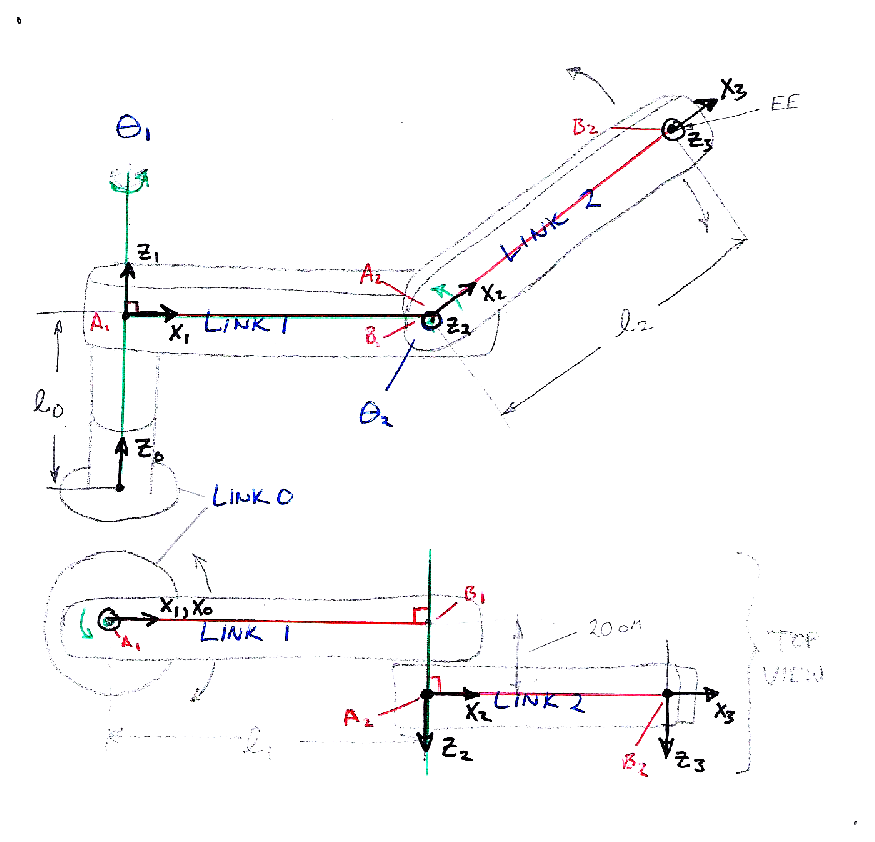
\includegraphics[width=3.25in]{figs03/00412.eps}
% \end{tabular}

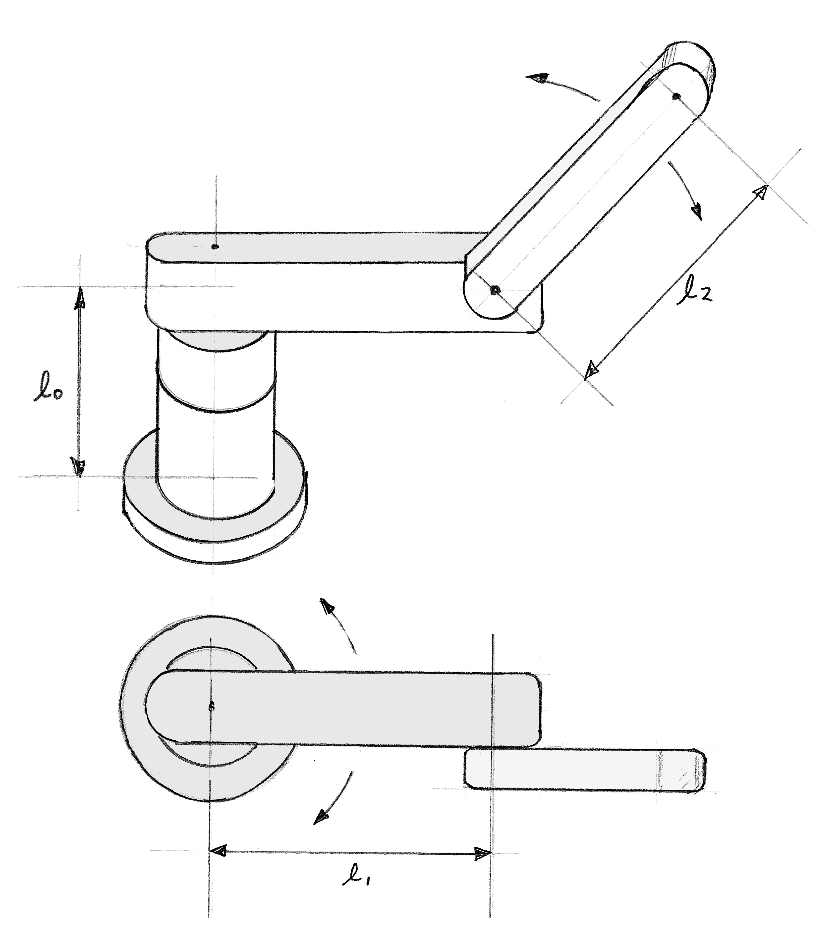
\includegraphics[width=3.25in]{figs03/00715_A.eps}

\begin{tabular}{cc}
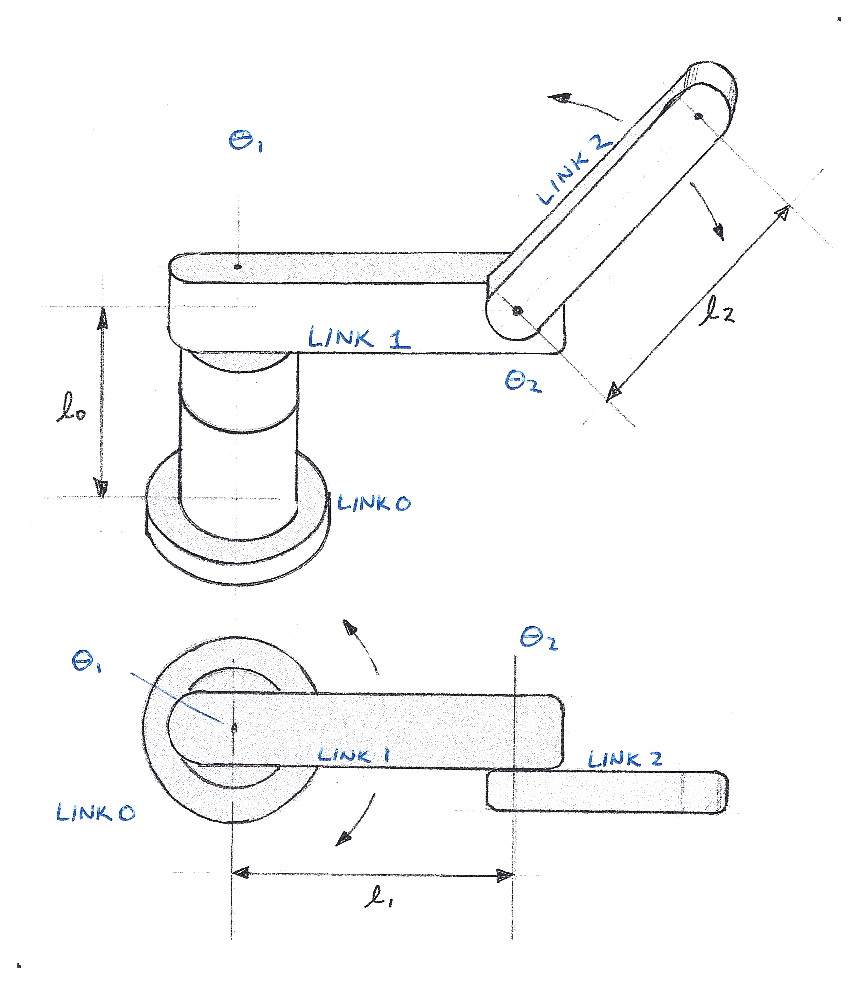
\includegraphics[width=3.25in]{figs03/00715_B.eps}
&
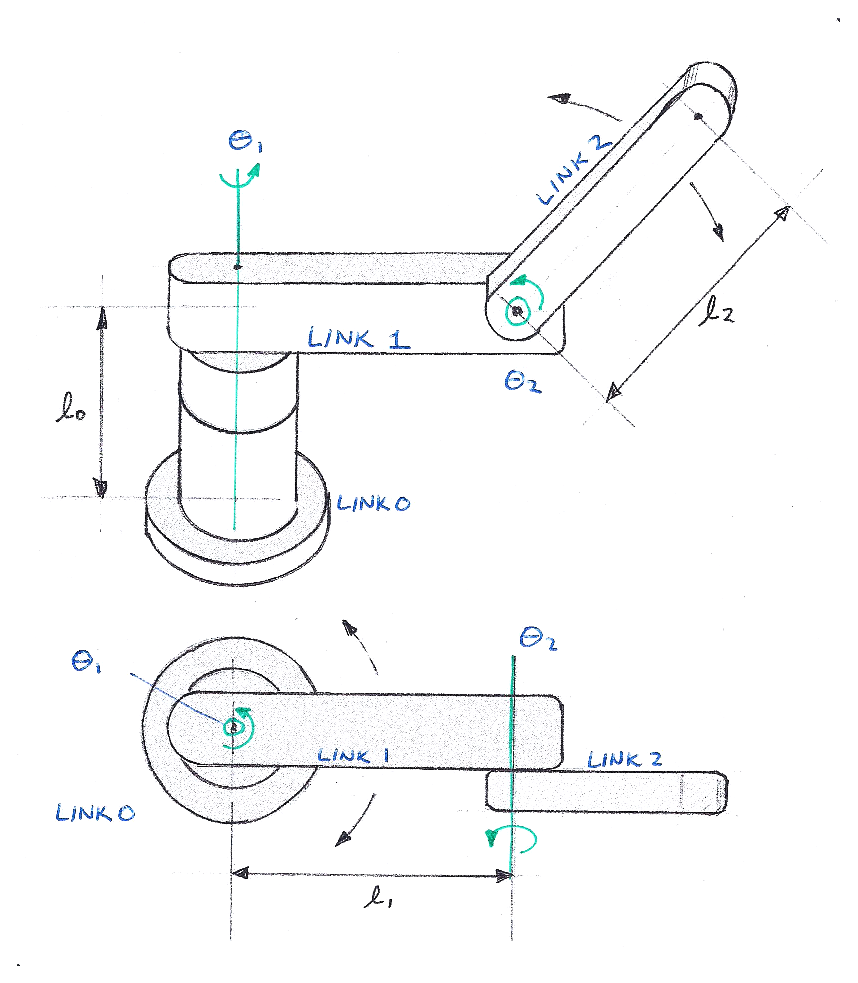
\includegraphics[width=3.25in]{figs03/00715_C.eps}
\end{tabular}
\end{Example}

\begin{ExampleCont}
\begin{tabular}{cc}
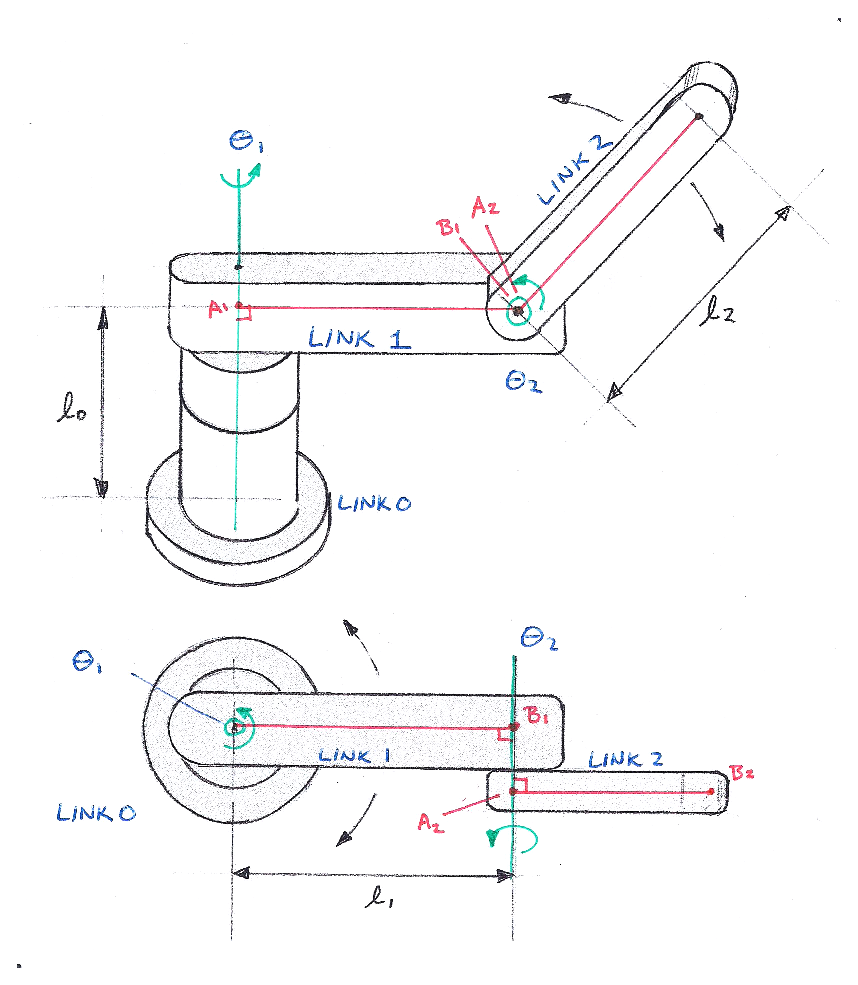
\includegraphics[width=3.25in]{figs03/00715_D.eps}
&
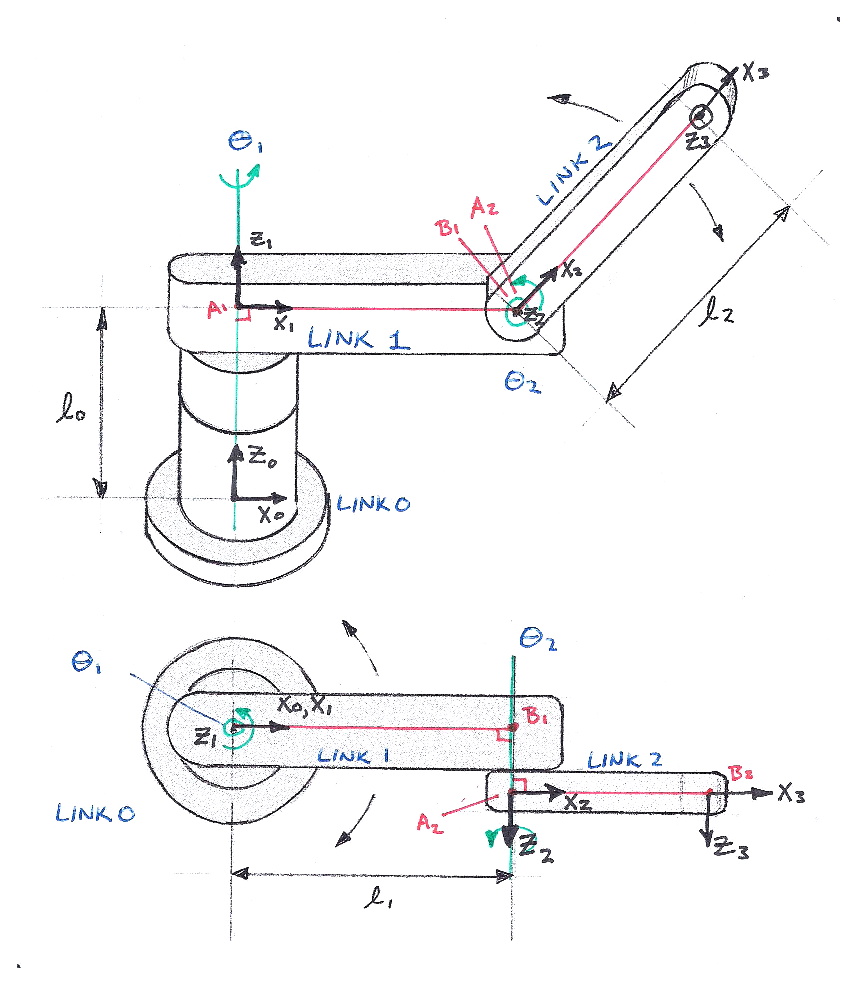
\includegraphics[width=3.25in]{figs03/00715_E.eps}
\end{tabular}


Second we identify the joint axis lines and choose directions of rotation around them (for rotary joints) which we denote to be positive (green).

Third, we draw in the common normals between the identified joint axes (red).

Finally, we identify the origins of each link frame, draw in $z_i$ pointing so that positive rotation follows the RHR, and draw $x_i$ along the common normal to the next axis (black).

A simplified stick figure (below) can sometimes help in visualizing the frame assignments:

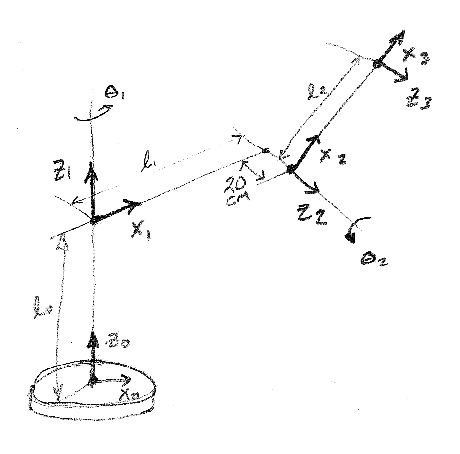
\includegraphics[width=72mm]{figs03/00885.eps}

\end{ExampleCont}
%%%%%%%%%%%%%%%%%%%%%%%%%%%%%%%%%%%%%%%%%%%%%%%%%%%%%%%%%%%%%%%%%%%%%%%%%%%%%%%%%%%%%%
%%%%%%%%%%%%%%%%%%%%%%%%%%%%%%%%%%%%%%%%%%%%%%%%%%%%%%%%%%%%%%%%%%%%%%%%
%
%       Example:  Link Frame Assignments: 6 DOF:   Stanford Arm
%
\begin{Example}

This example considers the 6 DOF arm designed by Vic Scheinman and Bernard Roth, the ``Stanford Arm".   The series of four drawings shows the steps in analyzing and applying frames to the arm.   Following the steps above in Section \ref{Steps}.

1) Understand the geometry and dimensions of the mechanism.  The first drawing indicates only the shape and motions of the arm.

2) In step two we number the links and joints.  It turns out that numbering the Joints is most important and we skip explicitly numbering the joints here. We add some dimensions for the shoulder height, $L_1$ and the shoulder offset $S$.

3) In green in the second drawing,  we highlight the directions we will consider positive motion,

4) This arm features all intersecting axes (to simplify the equations).  In drawing 3, we show in red CN vectors obtained by crossing sequential axes.

5) In drawing 4 we assign a link frame to each axis according to Step 5 of Section \ref{Steps}.

1) 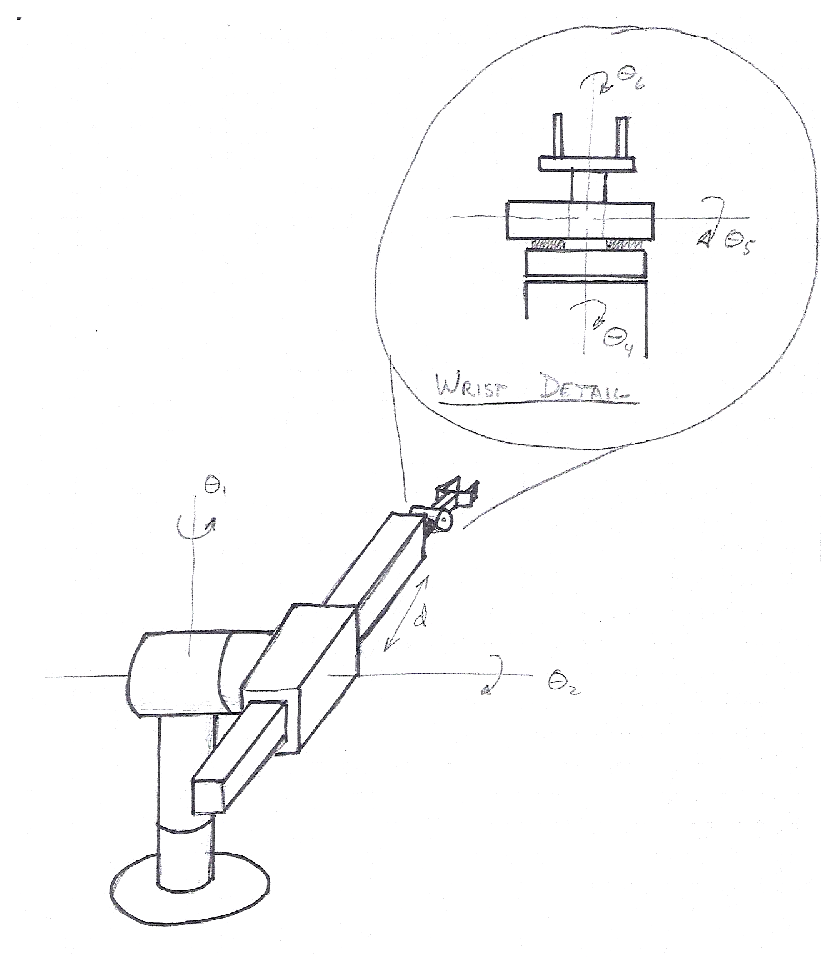
\includegraphics[width=3.2in]{figs03/00416.eps}
2) 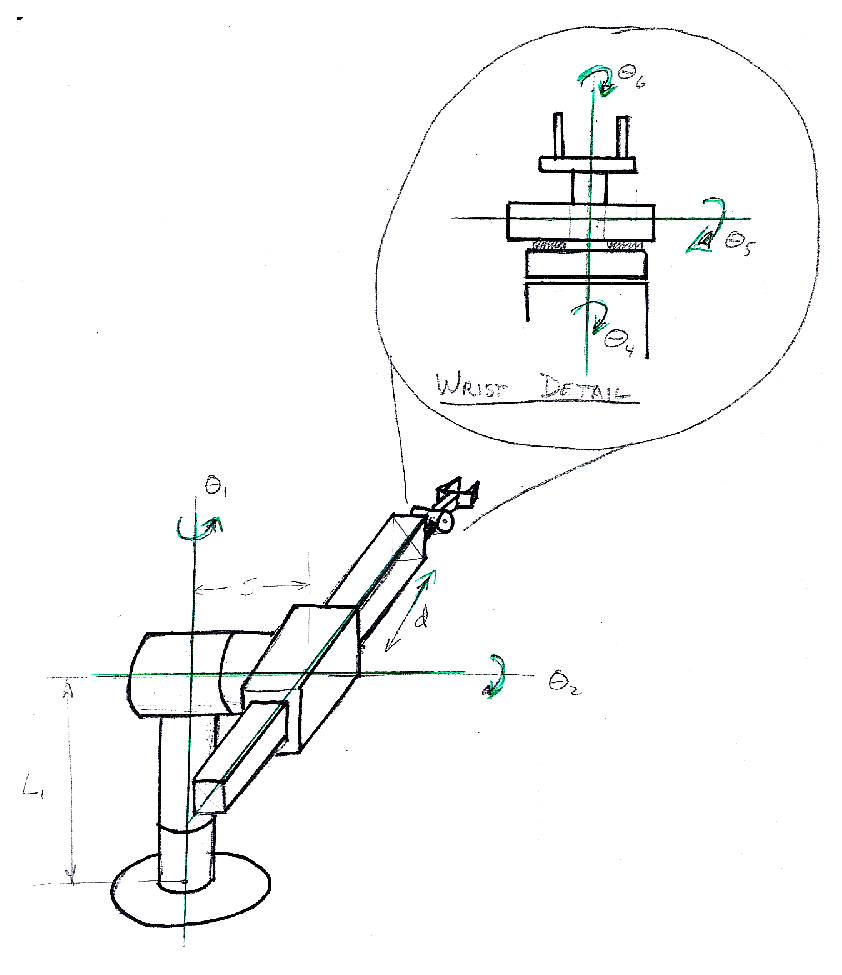
\includegraphics[width=3.2in]{figs03/00417.eps}\\
3) 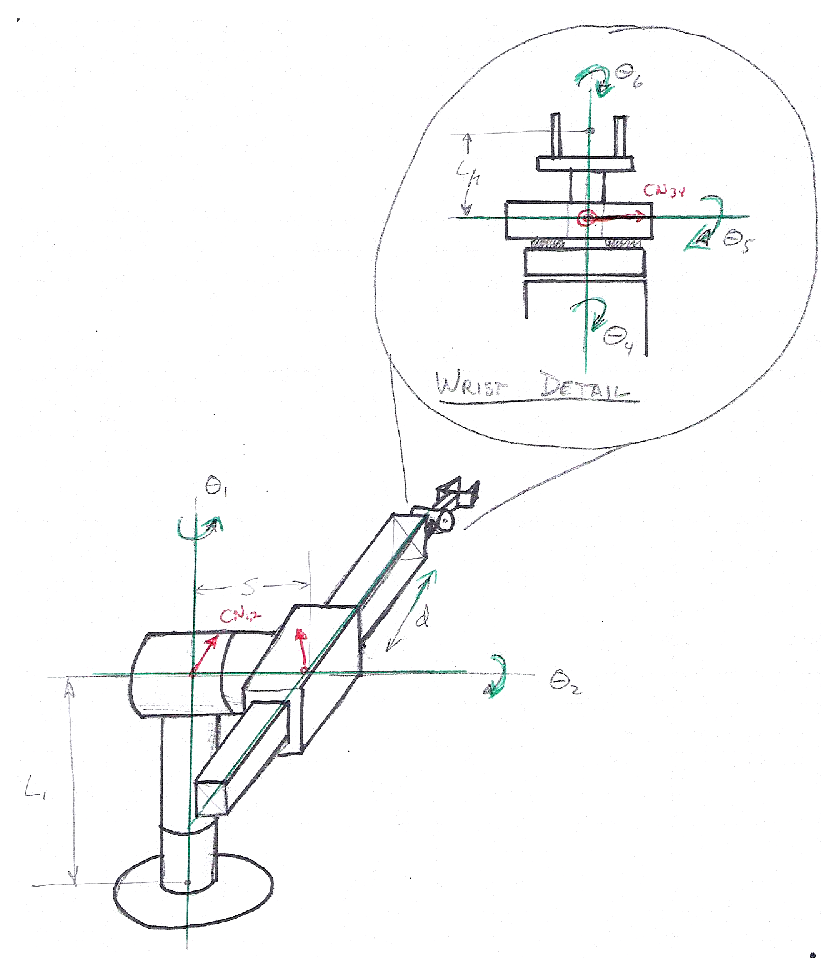
\includegraphics[width=3.2in]{figs03/00418.eps}
4) 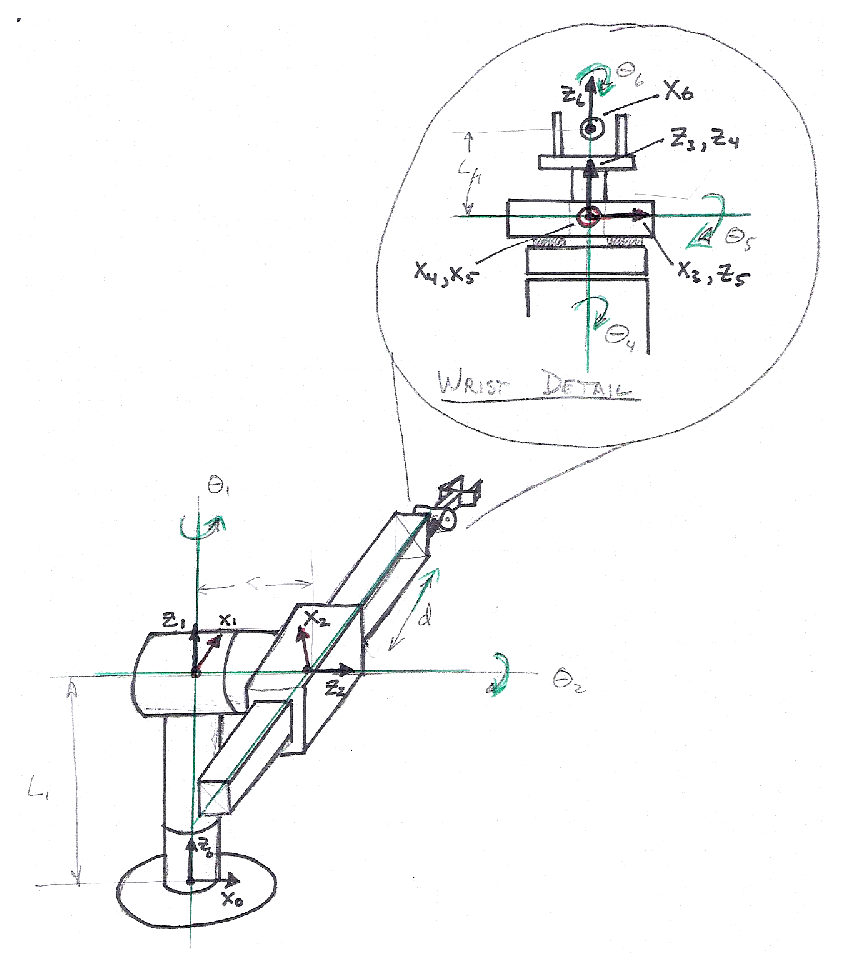
\includegraphics[width=3.2in]{figs03/00419.eps}

\label{FKex2}
\end{Example}



\section{Denavit Hartenberg Parameters}

In 1955 Denavit and Hartenburg created a standardized way to derive transforms from one link to another in a serial chain.  Once frames have been assigned to each link as described above, for each link, we will be able to identify two specific rotations and two translations which uniquely define the relationship between the links.  Of the four Denavit-Hartenberg (DH) parameters, three are fixed constants due to the rigid body nature of the link.  A fourth is a variable which specifies the relative motion between the link and the next link.  For rotary joints that variable is $\theta_N$ and for prismatic joints, that variable is $d_N$.  The definition of the four DH parameters are now given.    A very nice video illustration of the DH parameters is available at the wikipedia page for ``Denavit-Hartenberg Parameters".

\subsubsection{Composition of parameters}

\begin{figure}\centering
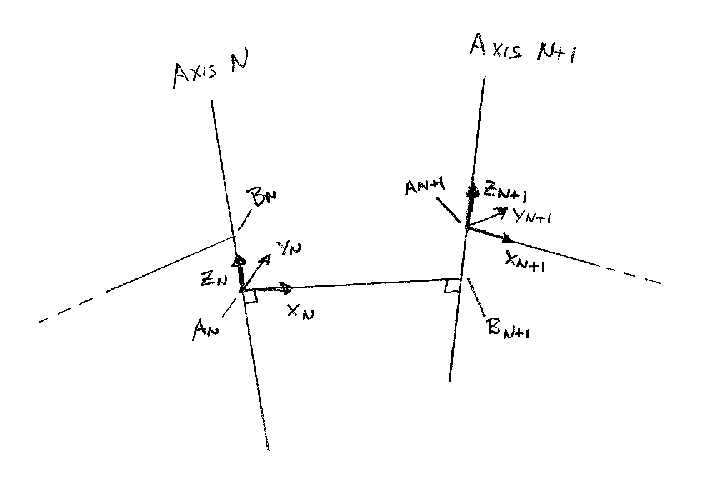
\includegraphics[width=3.5in]{figs03/00340.eps}
\caption{Virtual links with link frames fixed in both position and orientation.}\label{VirtualLinkswFrames}
\end{figure}

We use the DH parameters to describe the spatial relationship between frame $N-1$ and frame $N$.    Notice that a series of axes and CNs forms a continuous path from one link frame origin to the next.    We will follow this path through its twists and turns and describe each translation and rotation with a single DH parameter.  Each DH parameter represents a rotation or a translation about a single known axis.   Since the origin of Frame $N-1$ is $A_{N-1}$ we start there  and work our way to the origin of the next frame.   Refering to Figure \ref{VirtualLinkswFrames}, we rotate by the {\bf link twist}:  $\mathrm{Rot}(\hat{x},\alpha_{N-1})$, then translate by the {\bf link length}: Trans$(\hat{x},a_{N-1})$, then rotate by the {\bf joint angle}: Rot$(\hat{z}, \theta_N)$, and finally translate by the {\bf joint offset}: Trans$(\hat{z}, d_N)$.   Note that the relationship between link $N-1$ and link $N$ is described by parameters with a mix of subscripts.   The Denavit Hartenberg parameters can be visualized in
Figure \ref{CraigPaulLinkFrames}.

For the common case of rotary joints,  $a_{N-1}, \alpha_{N-1}, d_N$ will be fixed constants, dependent on the geometric design of the arm, and $\theta_N$ will be a variable joint angle.   Some arms include prismatic joints in which $\theta_N$ is a constant and $d_N$ is a variable.   In evaluating the link transform we typically replace all constant parameters with their measured or design values and keep the single variable parameter in DH form.     In rare cases, a joint includes two degrees of freedom such as a cylindrical shaft which can rotate as well as translate\footnote{See for example, the last two degrees of freedom of the SCARA arm.}.   In this case it is best to abstract that joint into two separate joints, one for rotation and one for translation.

Our strategy will be to multiply together 4x4 homogeneous transforms for each of the elemental displacement and rotations above which make up the virutal link.   To keep the notation under control we will use the following shorthand:

\[
 c\theta_j \equiv c_j \equiv cos(\theta_j)
\]
\[
s\theta_j \equiv s_j \equiv sin(\theta_j)
\]


The complete transform is then
\[
^{N-1}_NT =  \mathrm{Rot}(\hat{x},\alpha_{N-1})\mathrm{Trans}(\hat{x},a_{N-1})\mathrm{Rot}(\hat{z}, \theta_N)\mathrm{Trans}(\hat{z}, d_N)
\]
or equivalently

\[
^{N-1}_NT =  \mathrm{Rot}(\hat{x},\alpha_{N-1})\mathrm{Trans}(\hat{x},a_{N-1})\mathrm{Rot}(\hat{z}, \theta_N)\mathrm{Trans}(\hat{z}, d_N)
\]

\[
= \left[
   \begin{array}{cccc}
    1     &     0     &     0     &      0   \\
    0     &     c\alpha_{N-1}     &     -s\alpha_{N-1}     &      0   \\
    0     &     s\alpha_{N-1}     &      c\alpha_{N-1}     &      0   \\
    0     &     0     &     0     &      1   \\
   \end{array}
  \right ]
   \left[
   \begin{array}{cccc}
    1     &     0     &     0     &      a_{N-1}   \\
    0     &     1     &     0     &      0   \\
    0     &     0     &     1     &      0   \\
    0     &     0     &     0     &      1   \\
   \end{array}
  \right ]
   \left[
   \begin{array}{cccc}
    c\theta_N     &     -s\theta_N    &     0     &      0   \\
    s\theta_N     &      c\theta_N    &     0     &      0   \\
    0     &     0     &     1     &      0   \\
    0     &     0     &     0     &      1   \\
   \end{array}
  \right ]
   \left[
   \begin{array}{cccc}
    1     &     0     &     0     &      0   \\
    0     &     1     &     0     &      0   \\
    0     &     0     &     1     &      d_N   \\
    0     &     0     &     0     &      1   \\
   \end{array}
  \right ]
  \]


or equivalently

\[
^{N}_{N+1}T =  \mathrm{Rot}(\hat{x},\alpha_{N})\mathrm{Trans}(\hat{x},a_{N})\mathrm{Rot}(\hat{z}, \theta_{N+1})\mathrm{Trans}(\hat{z}, d_{N+1})
\]

\[
= \left[
   \begin{array}{cccc}
    1     &     0     &     0     &      0   \\
    0     &     c\alpha_{N}     &     -s\alpha_{N}     &      0   \\
    0     &     s\alpha_{N}     &      c\alpha_{N}     &      0   \\
    0     &     0     &     0     &      1   \\
   \end{array}
  \right ]
   \left[
   \begin{array}{cccc}
    1     &     0     &     0     &      a_{N}   \\
    0     &     1     &     0     &      0   \\
    0     &     0     &     1     &      0   \\
    0     &     0     &     0     &      1   \\
   \end{array}
  \right ]
   \left[
   \begin{array}{cccc}
    c\theta_{N+1}     &     -s\theta_{N+1}    &     0     &      0   \\
    s\theta_{N+1}     &      c\theta_{N+1}    &     0     &      0   \\
    0     &     0     &     1     &      0   \\
    0     &     0     &     0     &      1   \\
   \end{array}
  \right ]
   \left[
   \begin{array}{cccc}
    1     &     0     &     0     &      0   \\
    0     &     1     &     0     &      0   \\
    0     &     0     &     1     &      d_{N+1}   \\
    0     &     0     &     0     &      1   \\
   \end{array}
  \right ]
  \]

Each of these four matrices is a function of one of the four DH parameters.   We can then multiply them together to get a single matrix which represents the link.

\subsubsection{Generalized Link Transformation}
By multiplying all four matrices together we get the following transform for any link which has DH parameters:
\begin{equation}\label{DHLinkTransform}
^{N-1}_NT = \left [
  \begin{array}{cccc}
  c\theta_N	          & -s\theta_N	             &     0         &   a_{N-1}	\\
  s\theta_Nc\alpha_{N-1}  &  c\theta_Nc\alpha_{N-1}  & -s\alpha_{N-1}  & -s\alpha_{N-1}d_N  \\
  s\theta_Ns\alpha_{N-1}  & c\theta_Ns\alpha_{N-1}   & c\alpha_{N-1}   & c\alpha_{N-1}d_N  \\
   0 & 0 & 0 & 1
  \end{array}
\right ]
\end{equation}

The reader can derive the corresponding matrix for $^{N}_{N+1}T$.


\subsection{Combining links into a chain}

Once we have $^{N-1}_NT$ for all of the links, we multiply them together to get the full forward kinematics model. For example in a three link robot we would have
\[
^0_3T = \;^0_1T \;^1_2T \;^2_3T
\]

Usually it is possible and desirable to multiply them together in symbolic form.    We will bring this process together in the next section.

\subsection{Summary of Forward Kinematics Analysis Part 2}\label{DH_Steps}
\begin{enumerate}
\item Derive the Denavit Hartenberg parameters, $a_N, \alpha_N, d_N, \theta_N,$ from your assigned link frames as follows:

$a_N$ is the distance from $A_N$ to $B_{N+1}$.  This is the distance along the CN from $Z_N$ to $Z_{N+1}$.  $a_N$ is refered to as the ``link length" (see Figure \ref{VirtualLinksCN} and Figure \ref{DHStepsSummary2} D and E).

$\alpha_N$ is the angle between Axis $N$ and Axis $N+1$ about the common normal.  This is the angle between $Z_N$ and $Z_{N+1}$ about $X_N$ in the RHR sense.   $\alpha_N$ is called the ``link twist".

$d_N$ is the distance from $B_N$ to $A_N$.   This is the distance from $X_{N-1}$ to $X_N$ along $Z_N$.   $d_N$ is referred to as the ``joint offset".

$\theta_N$ is the angle between CN$_{N-1}$ and CN$_{N}$ around Axis $N$.  This is the angle between $X_{N-1}$ and $X_N$ around $Z_N$.   $\theta_N$ is refered to as the ``joint angle".

\item Use equation \ref{DHLinkTransform} to compute the link transform for each link


\item Multiply all the link transforms together.

\end{enumerate}





%%%%%%%%%%%%%%%%%%%%%%%%%%%%%%%%%%%%%%%%%%%%%%%%%%%%%%%%%%%%%%%%%%%%%%%%
%
%       Example:  DH parameters and Link Transforms: 3DOF
%
\begin{Example}
Find the 4x4 matrix representing the forward kinematic equations of the manipulator of Example \thechapter.\ref{FKex1}.
\vspace{0.075in}

Step 1.  Referring to the procedure of Section \ref{DH_Steps}

\begin{tabular}{|c|c|c|c|c|} \hline
$N$	&  $\alpha_{N-1}$   &  $a_{N-1}$    	& $d_N$		&  $\theta_N$  	\\ \hline
1	&     0        &     0			&  $l_0$	&  $\theta_1$  	\\ \hline
2	&   $90^{\circ}$	& $l_1$	&  20cm		&  $\theta_2$  		\\ \hline
3	&   0	&    $l_2$ 			&  0		&    0         	\\ \hline
\end{tabular}

\vspace{0.075in}

Step 2

Referring to Equation \ref{DHLinkTransform}

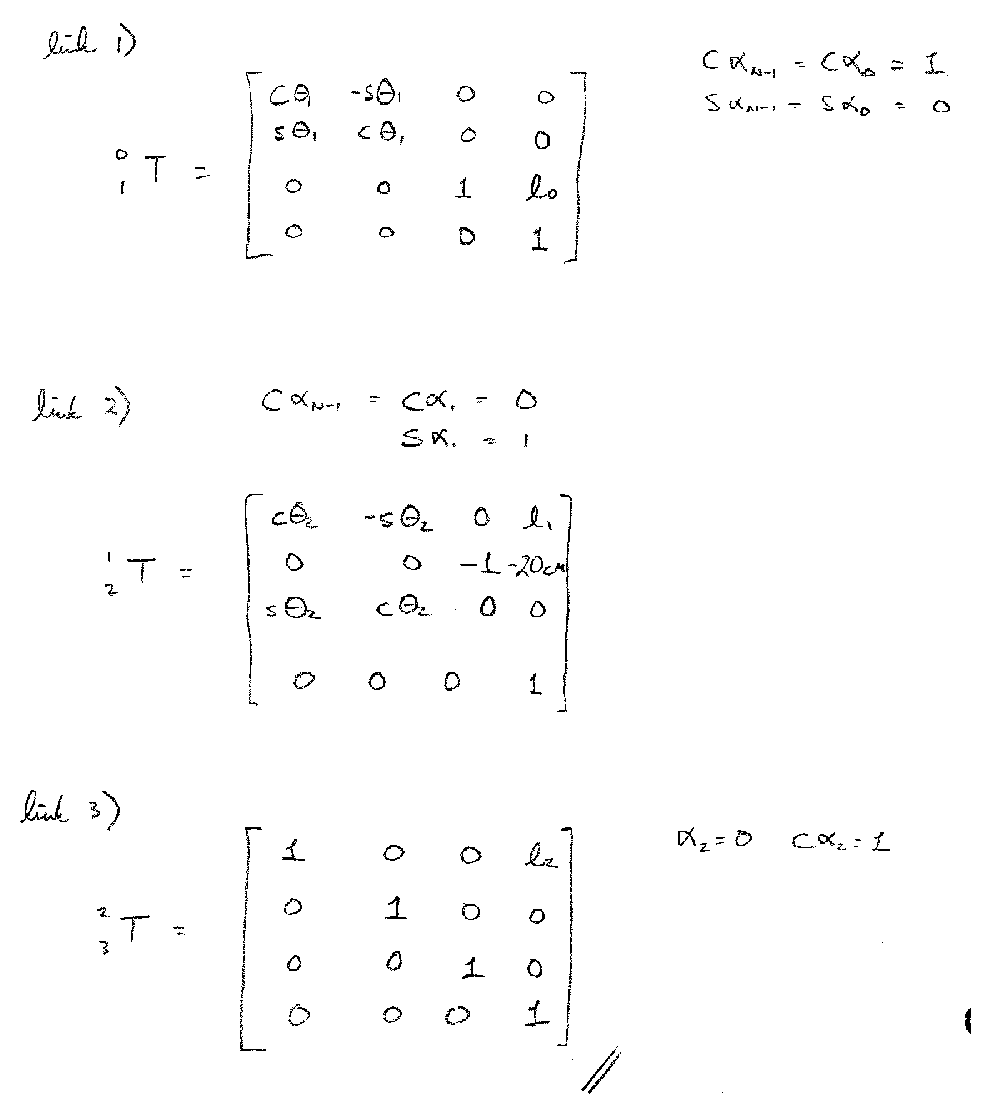
\includegraphics[width=5.0in]{figs03/00413.eps}
\end{Example}

\begin{ExampleCont}
Step 3

Now multiplying the three matrices together we get:

\includegraphics[width=5.0in]{figs03/00414.eps}

\includegraphics[width=5.0in]{figs03/00415.eps}

\end{ExampleCont}
%%%%%%%%%%%%%%%%%%%%%%%%%%%%%%%%%%%%%%%%%%%%%%%%%%%%%%%%%%%%%%%%%%%%%%%%%%


\begin{Example}
Find link frame assignments and Denavit Hartenberg parameters for the Rosheim Prehensile Wrist\footnote{Mark Rosheim, ``Robotic Wrist Actuators,''  John Wiley \& Sons, 1989.}.   The following interesting wrist mechanism has an extraordinary range of pitch orientations.

\includegraphics[width=5cm]{figs03/00420.eps}\includegraphics[width=7.5cm]{figs03/rosheim_pre_photo.eps}

\end{Example}

\newpage
\begin{ExampleCont}
Following the steps outlined above:

1) Understand the geometry and dimensions.   First, we arbitrarily identify the bottom of the rectanglar solid below the first bevel gears as a reference plane (i.e. we will locate Frame 0 there in the next step).  We draw diagonals in that plane to locate its center.  We also extend the joint axis lines through the joints and give names to the dimentions between them:



2) Number the Links and Joints.   Furthermore, the Wrist roll axis intersects the first horizontal axis (which we will call joint 2 in the next step) so that link 1 has zero length:

1) \includegraphics[width=5.38cm]{figs03/00421.eps} 2) \includegraphics[width=5.38cm]{figs03/00422.eps}

\end{ExampleCont}

\newpage
\begin{ExampleCont}
3) Identify axes of motion.  This is a bit tricky since the ``Pitch Transfer Gears" demand that some of the joints do not move independently.  However for now we will ignore the pitch transfer gears and consider the two axes to be independent joints.  We will ignore the sign convention which places the $Z$ axis along the direction of positive motion and simply point them to the left and up.

4) Draw common normals.   The common normal between $Z_0$ and $Z_1$ is zero length.  The CN between $Z_1$ and $Z_2$ is also zero length.   The CN from $Z_2$ to $Z_3$ is the line up the center of the drawing of length $l_2$.  The CN between axis $Z_3$ and $Z_4$ is zero length.

5) Assign a frame to each link.   Note that $F_0$ could go anywhere on the ``Wrist roll" body, but we place it  along the center axis for convenience.  Note that when we move around the Wrist roll axis, $F_0$ stays where it is and $F_1$ moves relative to it.

\includegraphics[width=5.38cm]{figs03/00423.eps}
\vspace{0.25in}

6) Following the procedures of Section \ref{DH_Steps}, we obtain
\vspace{0.25in}

\begin{tabular}{|c|c|c|c|c|} \hline
$N$	&  $\alpha_{N-1}$   &  $a_{N-1}$    	& $d_N$		&  $\theta_N$  \\     \hline
1	&   0 		    &    0 	    	&  $l_1$	&    $\theta_W$        \\ \hline
2	&   $\pi/2 $	    &    0       	&   0		& $\pi/2 + \theta_p$        	\\ \hline
3	&   0		    &   $l_2$		&  0		& $-\pi/2 + \theta_p$		\\ \hline
4	&   $-\pi/2 $       &   0		&  $l_3$	& $\theta_4$       		\\ \hline
\end{tabular}

Note that joints 2 and 3 form a single degree of freedom driven by $\theta_p$ because they are coupled together by the pitch transfer gears.

\end{ExampleCont}


\section{Spaces}

We have seen that the forward kinematics analysis generates a 4x4 matrix which is a function of $N$ variables where $N$ is the number of joints.   As the joints move to different values, the 4x4 matrix specifies different positions and orientations in the task space corresponding to a frame on the last link usually known as the end effector.

Although this matrix maps points in the end effector coordinate system to the base coordinate system, it is sometimes useful to think of this matrix as a description of a mapping from a set of joint values to an end effector configuration.   For a manipulator with $N$ joints, the joint values form a point in a $N$ dimensional space we call the {\it Joint Space}.

The 4x4 matrix $^0_NT$ gives us a rotation matrix and X,Y,Z coordinates of the end effector.  This is termed a ``configuration" of the manipulator end effector.   We commonly derive three orientation parameters such as roll, pitch, yaw, angles from the upper 3x3 part of $^0_NT$ to give six numbers which characterize the end effector configuration:

\begin{equation}
\left [
   \begin{array}{c}
	    X \\ Y \\ Z \\ \mathrm{roll} \\ \mathrm{pitch} \\ \mathrm{yaw}
   \end{array}
\right ]
\end{equation}

The above six numbers define a point in {\it End Effector Space}. End Effector Space is sometimes called ``Task Space" since it is a natural space in which to represent tasks or ``Configuration Space" although this term has a slightly different meaning in the context of motion planning.

As a manipulator moves around, a point moves around in joint space representing the values of its joints, and another point moves around in end effector space representing the configuration of the end effector.  As we shall see in the next chapter, there may be more than one joint space point which corresponds to the same end effector point, but there is always exactly one point in end effector space for each point in joint space.

Another relevant space is {\it Actuator Space}.   In most serial robots the actuators are located directly on each joint and actuator motion is a linear function of or is equal to the joint motion.   However in certain designs, such as the Yakusawa Motoman L-3, actuators may drive the joints through linkages and therefore move somewhat differently than the joints of the serial chain.  For good discussion of this consult Chapter 3 of Craig.


\newpage
\section{A further look at  the DH notation}
(The following section may be skipped without loss in future chapters)

\subsection{Structure of the Link Transform}

We can obtain some insight into the computation of link transformations by grouping the terms as shown in Figure \ref{LinkTransformBlobs}.  The clusters in Figure \ref{LinkTransformBlobs} represent blocks of terms which depend on a specific DH parameters.  Often, with industrial manipulators,
\[
\alpha_{i-1} = \{ 0, \pm \frac{\pi}{2}, \pi \}
\]
because they are easier to design and manufacture that way.   For these cases, we can see that the final expression for the link transform is simplified by $\cos(\alpha_{i-1}) = \{0,\pm1\}$.

Finally, we can classify the DH parameters into ones describing the {\it structure} of the link ($\theta_i, d_i$) versus the {\it relationship} with the next link ($\alpha_{i-1}, a_{i-1}$).  Each of these two classes has one rotational and one translational parameter:

\begin{center}
\begin{tabular}{r|cc}
            & Translation & Rotation \\ \hline
Structure   &  $a_{i-1}$ & $\alpha_{i-1}$  \\
Relationship &  $d_i$      & $\theta_i $    \\

\end{tabular}
\end{center}


\begin{figure}
\includegraphics[width=100mm]{figs03/00712.eps}
\caption{Different term types in the DH Link Transform). Matrix elements have dependencies on link {\it relationship} ($\theta_i, d_i$) or link {\it structure} ($\alpha_{i-1}, a_{i-1}$).}\label{LinkTransformBlobs}
\end{figure}


\subsection{Craig's vs. Paul's Transforms}\label{CraigVsPaul}

The first textbook on robot manpiulation was ``Robot Manipulators, Mathematics, Mechanics, and Control," by Richard Paul of the University of Pennsylvania (MIT Pres, 1981).    This book was very influential in starting research and courses around the world on robotic manipulation.   However, Paul used a slightly different variation on the Denavit Hartenberg method which results in different description of links.    In looking at the robotic manipulation literature, a researcher will still encounter work done in Paul's notation.

Both Craig and Paul's systems use the same DH parameters.  The key difference is that Paul's system puts the origin of frame N at the end of the link (point $B_{N+1}$ as defined in this chapter). Thus, different DH parameters are used in Paul's link description (Figure \ref{PaulTransformBlobs}).


\begin{figure}\centering
\includegraphics[width=60mm]{figs03/00713.eps}
\caption{Link transform for Paul's variation on the DH method.  Note different subscripts. Term types in the DH Link Transform similar to Figure \ref{LinkTransformBlobs}. }\label{PaulTransformBlobs}
\end{figure}


Paul's transform selects different DH parameters to represent the structure and relationships of the links:

\begin{center}
Paul's Link Parameters \\
\begin{tabular}{r|cc}
            & Translation & Rotation \\ \hline
Structure   &  $a_{i}$ & $\alpha_{i}$  \\
Relationship &  $d_i$      & $\theta_i $    \\
\end{tabular}
\end{center}

The obvious advantage of Paul's method is that subscripts are more consistent within the transform for each link.  However it has the non-intutive notion that the origin of Frame $N$ lies on axis $N+1$.  Craig's method has the more intuitive notion that  link frame $N$ is at the beginning of the link, located on axis $N$, but requires mixing of indeces in the link transform.  The two link frame assignment methods are summarized in Figure \ref{CraigPaulLinkFrames}.

\begin{figure}
\includegraphics[width=150mm]{figs03/00714.eps}
\caption{Different link frame assignments (within the same DH parameters) for Craig (bottom) and Paul's (top)  methods.}\label{CraigPaulLinkFrames}
\end{figure}



%
% \section{Summary of Notation}
%
% % Summary of Notation for Chapter  03

  % Forward Kinematics
 %  Robotics Text  by Jacob Rosen and Blake Hannaford
% (c) 2007  Jacob Rosen and Blake Hannaford
%

\chapter{Inverse Kinematics}



\section{Problem Statement and Learning Objectives}
% Problem Statement and Learning Objectives for Chapter 04
\paragraph{Problem Statement}
  
The inverse kinematics problem is to find the joint values for a given end effector configuration.  The solution to this problem is needed for most practical applications of serial robot arms. 

  
\paragraph{Learning Objectives}
Upon completing this Chapter, the reader should

\begin{itemize}
	\item Be able to plot the workspace of a serial manipulator with or without joint limits.
	\item Be able to solve for the joint angles of a planar robot given the end effector $x,y$ position and orientation.
	\item Be able to solve for the joint angles of a spatial 3 DOF robot given the $x,y,z$ position of the end effector.
	\item Be ready to tackle full scale inverse kinematics problems if sufficient time is available. 
\end{itemize}


\section{Overview}

We can express the forward kinematic problem as
\[
f(\theta) = {^0_6}T
\]
Then, to find the joint angles which correspond to a desired end effector configuration, we need to solve the inverse of this problem, the {\it Inverse Kinematic Problem}
\[
\theta = f^{-1}(^0_6T_d)
\]
where the $d$ subscript indicates the ``desired" end effector configuration.  Being able to solve the inverse kinematic problem is thus very important for automatic applications of robot manipulators since the control system must know the joint angles, $\theta$, in order to move the end effector to $^0_6T_d$.

For serial kinematic chains, this problem is harder than the forward kinematic problem.  Among the significant issues are:
\begin{itemize}
	\item Existence of solutions
	\item Multiple solutions
	\item How to find the solution(s)
\end{itemize}




\subsection{Workspace}
A robot arm, just like the human arm,  can only reach a certain number of points.  Wrapped up in our inverse kinematics calculation is the question of whether or not the desired end effector configuration is actually reachable.  Our mathematics should tell us this automatically when we try to compute the joint angles or displacements.  Fortunately, it works out that for a solution to the inverse kinematics problem to exist,  $^0_6T_d$ must be in the {\it workspace } of the manipulator.  We will use two definitions of workspace:

\begin{enumerate}
	\item {\bf Dexterous Workspace}.  The subset of space in which the robot end effector (EE) can reach all orientations.
	\item {\bf Reachable Workspace}   The subset of space in which the robot end effector (EE) can reach at least one orientation.
\end{enumerate}

Note that the dexterous workspace is a subset of the reachable workspace.

\begin{Example}
Consider a two link planar robot with no joint limits:

\includegraphics[width=1.5in]{figs04/00425.eps}

Then the reachable workspace is:


\includegraphics[width=3.125in]{figs04/00426.eps}

and the dexterous workspace is the empty set.

\newpage


Now, if $l_1 = l_2 = 9$, the outer radius is the same, and


\includegraphics[width=3.75in]{figs04/00427.eps}

Now the RW is the same but the DW exists at a point at the origin where any orientation can be obtained.

\label{workspacedonut}
\end{Example}
\newpage
\begin{ExampleCont}

Now let's add a joint at the wrist

\includegraphics[width=1.5in]{figs04/00428.eps}


and set link lengths to $l_1 = 8,  = l_2 = 10 $.

\includegraphics[width=2.0in]{figs04/00429.eps}

Now the reachable and dexterous workspaces are the same.
\end{ExampleCont}


\paragraph{Joint Limits}

The joints in real mechanisms often cannot achieve rotations of $0-2\pi$ (or for that matter infinite displacements on prismatic joints!).  Thus joint limits
\[
\theta_{imin} \le \theta_i \le \theta_{imax} \qquad d_{imin} \le d_i \le d_{imax}
\]
contribute additional limits to the workspace.

Rotary Joints

Without joint limits, the 2-link planar robot makes a donut shaped reachable workspace in the task space (Example \thechapter.\ref{workspacedonut}).  In joint space, any point can be attained.  When joint limits are introduced, a rectangular solid is created defined by $\theta_{imin}$ and $\theta_{imax}$ for each dimension.   To convert this rectangular solid back to task space, we note that each edge of the solid corresponds to varying just one joint at a time.  The edges in the joint space thus become arcs in the task space.   For the 2 joint manipulator, these limits allow joint configurations inside the rectangle shown in Figure \ref{2LinkVisJointLimits}, right.

\begin{figure}\centering
\includegraphics[width =4.0in]{figs04/00444.eps}
\caption{Visualization of joint limits for a 2-link manipulator.}\label{2LinkVisJointLimits}
\end{figure}



Plotting the workspace can be tricky with joint limits.   One approach:
\begin{enumerate}
	\item Identify the corners (vertices) of the joint space rectangular solid.
	\item Plot a point in the task space for each vertex.
	\item Connect the points with arcs (use a compass to draw) around the joint axis to connect the vertices.
	\item Remember that some workspace boundaries may not occur at joint limits such as when the arm is fully stretched out.
\end{enumerate}



%%%%%%%%%%%%%%%%%%%%%%%%%%%%%%%%%%%%%%%%%%%  4.2
\begin{ExampleSmall}\label{2LinkJointLimits}
Consider a 2DOF planar manipulator with link lengths $l_1 = 4, l_2 = 1.5$.    Assume the joints are limited to
\[
0 \le \theta_1 \le 180^{\circ}   \qquad   -90^{\circ} \le \theta_2 \le 180^{\circ}
\]

Plot the reachable workspace.

\includegraphics[width=4.25in]{figs04/00445.eps}

\end{ExampleSmall}

%%%%%%%%%%%%%%%%%%%%%%%%%%%%%%%%%%%%%%%%%%%  4.3
\begin{ExampleSmall}
Same problem as previous example:  $l_1 = 3, l_2 = 1.5$.    Assume the joints are limited to
\[
45^{\circ} \le \theta_1 \le 135^{\circ}   \qquad   -45^{\circ} \le \theta_2 \le 90^{\circ}
\]
\includegraphics[width=4.25in]{figs04/00446.eps}
\end{ExampleSmall}


%%%%%%%%%%%%%%%%%%%%%%%%%%%%%%%%%%%%%%%%%%%   4.4
\begin{Example}
Generate top view and perspective view of the 3D workspace of the manipulator shown:

\includegraphics[width=2.5in]{figs04/00447.eps}

Where the joint limits are
\[
0 \le  \theta_1  \le 90^\circ     \qquad
2 <  d_2 < 4			 \qquad
-45^\circ  <  \theta_3 < 45^\circ
\]

First, we look at the plane containing the ``$d_2$" and the ``$l_3$" links (i.e. the vertical plane normal to $Z_2$.).

\includegraphics[width=4.25in]{figs04/00448a.eps}

Then by sweeping this planar workspace about $Z_1$, we generate the top view and perspective view.

\includegraphics[width=4.25in]{figs04/00448b.eps}


\end{Example}


%%%%%%%%%%%%%%%%%%%%%%%%%%%%%%%%%%%%%%%%%%%%   4.5
\begin{Example}
Draw the 2-D workspace of the planar manipulator drawn below:

\includegraphics[width=3.0in]{figs04/00250.eps}

Facts:
\begin{itemize}
        \item $45^{\circ} < \theta_1   < 90^{\circ}$
        \item $-90^{\circ} < \theta_2  < 0^{\circ}$
        \item $20^{\circ} < \theta_3   < 120^{\circ}$
        \item $l_1 = 5, \quad l_2 = 4, \quad l_3 = 3$
\end{itemize}

\subsection*{Solution:}

\includegraphics[width=3.5in]{figs04/00442.eps}

\end{Example}












\subsection{Multiple Solutions}

We will consider two important cases: first, when the number of degrees of freedom of the robot are equal to the number in the task, and second when the number of degrees of freedom in the robot are greater than in the task.

1) Consider a 2 link planar arm (Figure \ref{2link3link}, left).

\begin{figure}\centering
\includegraphics[width=75mm]{figs04/00716.eps} \hspace{0.1in}
\includegraphics[width=75mm]{figs04/00717.eps}
\caption{Planar manipulators with 2 links (left) and 3 links (right) pointing at the same goal point.}\label{2link3link}
\end{figure}


This arm has two joints and two links.   We consider its task to be completely specified by the position of its end effector in the plane.  Thus the number of degrees of freedom and the dimensionality of the task are both 2.
In this case there are a finite number of solutions (2) which are illustrated above.   The planar two-joint arm can reach the goal in two configurations referred to as ``elbow-up" and ``elbow-down."  Each of these configurations is a separate solution to the inverse kinematics problem.

2) Consider a 3-link planar arm with the same goal(Figure \ref{2link3link}, right).



In this case there are an infinite number of solutions (10 are shown).  The robot has three joints and therefore three degrees of freedom, but the task is still only two DOF.   This robot is thus underspecified --- a situation we call kinematic redundancy.  A robot with kinematic redundancy
can even move itself around (among the infinite number of solutions) without moving the end effector from the goal.  This is called self-motion.
% Kinematic redundancy will be considered in Chapter \ref {KinematicRedundancyChapter}.




\subsection{Methods of Solution}

There are three principal ways to obtain the inverse kinematics solutions:

\begin{enumerate}
	\item ``Closed Form":  An analytic expression for $\theta$ as a function of $^0_6T_d$ which includes all solutions.

	\item Numerical methods.

	\item Hybrid approach in which some degrees of freedom are solved in closed form and others numerically.

\end{enumerate}

We will concentrate here on the closed form solution.


There are two standard approaches to obtaining the closed form solution, the algebraic approach, primarily involving manipulation of the forward kinematic equations, and the geometric approach, in which the inverse kinematics problem is reduced to one or more plane geometry problems. However, unlike the forward kinematics problem, there is no straightforward procedure which can be followed to get analytical solutions.

%*******************************************************************************************************************
%
%
\section{Inverse Kinematics Tools}
\subsection{Inverse of a Homogeneous Transform}
Let's define two frames which are related by a translation $P_{1,2}$ and a rotation $^1_2R$ (Figure \ref{positionrotationoffset}).

\begin{figure}\centering
\includegraphics[width=2.5in]{figs04/00432.eps}
\caption{Two frames with a position offset, $P_{1,2}$ and a rotation offset ${^1_2R}$}\label{positionrotationoffset}
\end{figure}

If we represent this spatial relationship by a homogeneous transform, $T$, then it is reasonable to assume that an inverse, $T^{-1}$ must always exist

Q:  Why?

A:  One reason: a physical move can always be ``undone."   Another reason\footnote{J.M. McCarthy, ``Introduction to Theoretical Kinematics," MIT Press, 1990.},
eigenvalues of $T = 1, e^{j\theta}, e^{-j\theta}$, so their product, (the determinant) is always non-zero.

If the homogeneous transform is

\[
^1_2T =
\begin{bmatrix}
\begin{bmatrix}  &  &  \\  & ^1_2R&  \\ & & \\ \end{bmatrix}      &
 \begin{bmatrix}  \\ ^1P_{1,2} \\  \\ \end{bmatrix}            \\
 0 \quad 0 \quad 0      &   1
\end{bmatrix}
\]

then it is easy to show that its inverse is

\[
^1_2T^{-1} = ^2_1T =
\begin{bmatrix}
\begin{bmatrix}  &  &  \\  & ^2_1R&  \\ & & \\ \end{bmatrix}      &
 \begin{bmatrix}  \\ -^2P_{1,2} \\  \\ \end{bmatrix}            \\
 0 \quad 0 \quad 0      &   1
\end{bmatrix}
\]

where $^2_1R = {^1_2R}^T$ and $-^2P_{1,2} = {^2_1R}\left( -{^1P_{1,2}} \right )$


%%%%%%%%%%%%%%%%%%%%%%%%%%%%%%%%%%%%%%%%%%%%%%%%%%%%%%%%%%%%%%%%%%%%%%%%%%%%%%%%%%%%%%%%%%%%%%%%%%%%%%%%%%%%%%%%%%%
%%
%%    New quaternion material for inverse kinematics
%%
\subsection{Inverse of a Quaternion}

The inverse of a quaternion (Section \ref{QuaternionSection}), $q*$ ,is simply its conjugate, equation (\ref{quaternioninversedefinition}).

\[
q^* = \cos(\theta/2) - K_xi\sin(\theta/2) -K_yj\sin(\theta/2) - K_zk\sin(\theta/2) = (w,-x,-y,-z)
\]

\subsection{Inverse Sin and Cos}

The basic inverse trigonometric functions are often useful. Remember that they each have two solutions:
\[
\sin^{-1}(x) = \{\theta,\: \pi-\theta\} \qquad  \cos^{-1}(x) = \pm \theta
\]
and that they are only valid for
\[
-1 \leq x \leq 1
\]


\subsection{Atan2(y,x)}

We need a slightly more sophisticated form of the $\arctan()$ function to find angles.  Consider a trivial robot arm with a single link of unit length with a rotary joint at the origin.  If we pick a point on the unit circle, then the inverse kinematics problem is simply solved by the arctangent.  However, the arctan function domain is limited to the first and fourth quadrants:
\[
-\frac{\pi}{2} \leq \arctan(\frac{y}{x}) \leq \frac{\pi}{2}
\]

In real-world problems, we need to solve the inverse kinematics problem for any quadrant (Figure \ref{atan2figure}).

\begin{figure}\centering
\includegraphics[width=3.25in]{figs04/00435.eps}
\caption{Unlike the arctangent function, the {\tt atan2(y,x)} function returns a result in any quadrant, I-IV.}\label{atan2figure}
\end{figure}


The {\bf atan2(y,x)} function, also known as the four quadrant arctangent, returns an angle between 0 and $2\pi$ allowing the solution to occupy any of the four quadrants.



\subsection{Key Trigonometric Identities}

Some trig identities (which may have faded from your mind) will be very useful in solving inverse kinematics problems.

\subsubsection{Sum of Angles}
If $c_{12} = \cos(\theta_1 + \theta_2)$ and $s_{12} = \sin(\theta_1 + \theta_2)$, then
\[
c_{12} = c_1 c_2 - s_1 s_2
\]
and
\[
s_{12} = c_1 s_2 + s_1 c_2
\]

This offers a way to solve   the following problem which frequently comes up in inverse kinematics:

\begin{quotation}
``Given $k_1$, $k_2$, and $x$, solve
$x = k_1\cos(\theta_1) + k_2\sin(\theta_1)$ for $\theta_1$.''
\end{quotation}

Here is one way:

Let $r = \sqrt{k_1^2 + k_2^2}$ and let $\theta_2 = \mathrm{atan2}(k_1,k_2)$.  In other words
\[
k_1 = rs_2, \quad k_2 = rc_2
\]
Rewriting the problem with this change of variables and applying sum-of-angles:
\[
x = rs_2c_1 + rc_2s_1 = rs_{12}
\]
\[
\frac{x}{r} = \sin(\theta_1 + \theta_2) = s_{12}
\]
We can solve this with the inverse sine function, $\sin^{-1}()$, but there is a preference in the robotics literature to transform it further into an atan2() solution by:
\[
c_{12} = \pm\sqrt{1-s^2_{12}} = \pm\sqrt{1-\left ( \frac{x}{r} \right)^2}
\]
\[
\theta_1 + \theta_2 = \mathrm{atan2}(s_{12}, c_{12})
\]
\[
\theta_1 = \mathrm{atan2}\left ( \frac{x}{r},  \pm\sqrt{1-\left ( \frac{x}{r} \right)^2} \right ) - \mathrm{atan2}(k_1,k_2)
\]

Note that there are two solutions to this equation corresponding to the $\pm$ choice of the square root.

A  joint angle can only be a real number for a reachable pose.  For the real solution to exist, the argument of the square root must be real giving
\[
\frac{x^2}{r^2}\leq 1, \quad x^2 \leq r^2, \quad |x| \leq |r|, \quad |x| \leq +\sqrt{k_1^2+k_2^2}
\]

So, if $|x| > \sqrt{k_1^2+k_2^2}$, no solution exists.  This is a mathematical test we can apply during computation to check whether or not the manipulator is capable of reaching the desired point.   However this is not the only condition which must be met in practice because we are still considering the idealized case where the joints can take on any value. In real manipulators, joint limits prohibit some points from being reached even if the inverse kinematics solution exists.


\subsection{Law of Cosines}

\begin{figure}\centering
\includegraphics[width=3.5in]{figs04/00436.eps}
\caption{Triangle and notation for the Law of Cosines.}\label{LOC}
\end{figure}

This old workhorse is a way to solve a frequently arising problem in inverse kinematics when an arm has two parallel axes.  Considering a triangle as in Figure \ref{LOC}, the law of cosines states:
\[
r^2 = L_1^2+L_2^2-2L_1L_2\cos(\theta)
\]
for an alternate form, we can use the fact that  $\theta = \pi + \alpha$ to get
\[
r^2 = L_1^2 + L_2^2 + 2L_1L_2\cos(\pm \alpha)
\]
This has two solutions since $\cos(\alpha) = \cos(-\alpha)$.


\subsection{Manipulator Sub-Space}

When the robot has fewer than six DOF, but the task has six DOF, then there are no solutions to the general problem, but only special cases. However, it is often useful to specify a subspace of the full 6 DOF configuration space which has a dimensionality which matches the robot arm.  For example, if we restrict our desired EE positions to the plane, then a planar arm is capable of reaching them. This plane, embedded in the six DOF space of possible rigid body configurations, in an example of a manipulator sub-space.

Alternatively, we can think of a planar world in which the configuration of any object consists of the $x$ and $y$ positions, and $\alpha$, the orientation of the object.

\begin{ExampleSmall}\label{PlanarManipSS}
Consider the following arm in a planar world which can reach various $x, y$ positions, but has a fixed wrist so that frame 3 has a particular orientation depending on the angles $\theta_1$ and $\theta_2$. Because of this dependence, the arm can only reach two specific orientations corresponding to the ``elbow-up" and ``elbow-down" solutions.

\includegraphics[width=3.75in]{figs04/00437.eps}


Suppose our task is described by
\[
^0_3T =
\begin{bmatrix}
\begin{bmatrix}  &  &  \\  & ^0_3R&  \\ & & \\ \end{bmatrix}      &
 \begin{bmatrix} x \\ y \\ z=0 \end{bmatrix}            \\
 0 \quad 0 \quad 0      &   1
\end{bmatrix}
\]

Since there is no joint at the wrist of this robot, ${^0_3R} = {^0_3R}(x,y)$ is a multivalued function of $x, y$.   We call

\[
^0_3T_D(x,y) =
\begin{bmatrix}
\begin{bmatrix}  &  &  \\  & ^0_3R(x,y) &   \\ & & \\ \end{bmatrix}      &
 \begin{bmatrix} x \\ y \\  0  \\ \end{bmatrix}            \\
 0 \quad 0 \quad 0      &   1
\end{bmatrix}
\]
the ``Manipulator subspace."  In more detail, we can only reach two orientations in the $x,y$ plane so $^0_3R$ has the form
\[
{^0_3R}(x,y) =
   \begin{bmatrix}
          c\alpha	&   -s\alpha	&   0	\\
	  s\alpha	&    c\alpha	&   0	\\
	     0 		&     	0	&   1   \\
   \end{bmatrix}
\]
where $\alpha$ is a two-valued function of $x,y$.
If we use the algebraic approach, we would set up the problem:
\[
^0_3T_D(x,y) = {^0_1T}(\theta_1){^1_2T}(\theta_2){^2_3T}
\]
\end{ExampleSmall}

The manipulator sub-space is not always easy to find.  In the case of Example \thechapter.\ref{PlanarManipSS}, the inverse kinematics problem is more easily solved with a geometric approach and does not require a manipulator subspace anyway.  Sometimes 6 DOF robots are easier to solve than 5DOF robots because they do not require a manipulator subspace to be derived.





\subsection{Simultaneous Equations}

One problem which comes up frequently in inverse kinematics is simulataneous equations in the joint variables\footnote{Thanks to Prof. Pamela Bhatti.}.   For example,

\[
x = l_1c_1 + l_2c_{12}
\]
\[
y = l_1s_1 + l_2s_{12}
\]
where $c_{12} = \cos(\theta_1+\theta_2)$ (terms involving sums of two joint angles are common when two axes are parallel in a manipulator design).  The problem is to find $\theta_1$ when $\theta_2$ is known.

Use the sum-of-angles formulae to rewrite equations as

\[
x = l_1c_1 + l_2(c_1c_2 -s_1s_2)
\]
\[
y = l_1s_1 + l_2(c_2s_1 + s_2c_1)
\]

Now isolate the unknowns:

\[
x = (l_1+l_2c_2)c_1 - (l_2s_2)s_1
\]
\[
y = (l_1+l_2c_2)s_1 + (l_2s_2)c_1
\]


let $k_1 = (l_1+l_2c_2)$ and $k_2 = l_2s_2$ and place these equations into matrix form:

\[
\begin{bmatrix} x \\ y \end{bmatrix} =
\begin{bmatrix} k_1  & -k_2 \\ k_2 & k_1 \end{bmatrix}
\begin{bmatrix} c_1 \\ s_1   \end{bmatrix}
\]

Using standard $2\times2$ matrix methods to solve for $x,y$,

\[
\mathrm{determinant} = k_1^2 +k_2^2
\]
\[
c_1 = \frac {xk_1+yk_2}  {k_1^2 +k_2^2}
\]
\[
s_1 = \frac {yk_1-xk_2}  {k_1^2 +k_2^2}
\]

\[
\theta_1 = \mathrm{atan2}(yk_1-xk_2, \quad xk_1+yk_2)
\]
(Since the demoninators are always positive, we can drop them from the atan2. Also, note that
we need another equation to get $\theta_2$.)









\section{Algebraic Solution}

\subsection{Strategy}

The forward kinematics analysis of an all rotary  6DOF arm yields an equation
\[
^0_6T \quad = \quad ^0_1T(\theta_1) \quad ^1_2T(\theta_2) \quad ^2_3T(\theta_3) \quad ^3_4T(\theta_4) \quad ^4_5T(\theta_5) \quad ^5_6T(\theta_6)
\]
In the inverse kinematics version of the problem, ${^0_6T}$ is  known and we can call it ${^0_6T}_D$ (meaning desired), and the $\theta_i$ are unknowns.  The equation
\[
{^0_6T}_D = {^0_6T}
\]
is really 12 individual equations, one for each element of the first three rows.  On inspecting those 12 equations we might find one which can easily be solved for $\theta_1$ or perhaps a pair of equations which could jointly be solved for $\theta_1$.  But all of the other unknowns are mixed into complicated equations with no apparent solution.  However, when $\theta_1$ is solved,  $^0_1T(\theta_1)$ becomes a known matrix.  We can then write
% \[
%  ^0_1T(\theta_1)^{-1} \quad  ^0_6T \quad =  {^1_2T}(\theta_2) \quad {^2_3T}(\theta_3) \quad {^3_4T}(\theta_4) \quad {^4_5T}(\theta_5) \quad {^5_6T}(\theta_6)
% \]
\[
{^0_1T^{-1}}\;{^0_6T_D^{-1}} = {^0_1T(\theta_1)^{-1}}\;{^0_6T} \:
= \: {^1_2T}(\theta_2) \quad {^2_3T}(\theta_3) \quad {^3_4T}(\theta_4) \quad {^4_5T}(\theta_5) \quad {^5_6T}(\theta_6)
\]
which generates a fresh  set of 12 equations in which all the elements of the left hand side are knowns.    We may now find a new equation or set of equations which we can solve for $\theta_2$.   When $\theta_2$ is known, we can write
\[
 ^1_2T(\theta_2)^{-1} \quad {^0_1T}(\theta_1)^{-1} \quad {^0_6T}=   ^2_3T(\theta_3) \quad ^3_4T(\theta_4) \quad ^4_5T(\theta_5) \quad ^5_6T(\theta_6)
\]

Although there are several ``might"s in this description, because of the serial nature of the arms, this method works as described more often than one ``might" think.


\subsection{Examples}

\begin{Example}\label{ZYXWrist}
Consider a mechanism which corresponds to the $z,y,x$ Euler angles (Section \ref{ZYXEuler}).

\begin{center}
% \includegraphics[width=3.6in]{figs04/00438.eps}
\includegraphics[width=2.2in]{figs04/00710.eps}
\includegraphics[width=1.943in]{figs04/00711.eps}
\end{center}

This mechanism has three axes of rotation which intersect at a single point.  The axes are arranged so that the first rotation about $z$, moves the $x$ and $y$ axes for subsequent rotations which corresponds to the definition of Euler angles.  The last frame, frame 3, has no offset from the point where the axes intersect, so the homogeneous transform consists only of rotation with no translation. The amounts of rotation about $z,y,x$ are $A,B,C$.   Expanding the 3x3 rotation matrix of Section \ref{ZYXEuler} into a 4x4 homogeneous transform with zero translation, we get
\[
{^0_3T}(A,B,C)  =
\begin{bmatrix}
cAcB  &  cAsBsC-sAcC    &  cAsBcC+sAsC  & 0  \\
sAcB  &  sAsBsC+cAcC    &  sAsBcC-cAsC  & 0  \\
-sB   &  cBsC           &    cBcC       & 0  \\
0     &     0           &      0        & 1  \\
\end{bmatrix}
\]
The manipulator subspace for this manipulator is
\[
^0_3T_D =
\begin{bmatrix}
\begin{bmatrix}  &  &  \\  &  R &   \\ & & \\ \end{bmatrix}      &
 \begin{bmatrix} 0 \\ 0 \\  0  \\ \end{bmatrix}            \\
 0 \quad 0 \quad 0      &   1
\end{bmatrix}
\]
Where $R$ can be any rotation matrix because we can reach nearly any orientation with ZYX Euler angles (see below).   The inverse kinematics problem can then be set up to solve
\[
^0_3T_D = {^0_3T}(A,B,C)
\]
for $A,B,C$, given $^0_3T_D$,     Expanding this equation gives
\[
\begin{bmatrix}
r_{11}    & r_{12}  & r_{13} \\
r_{21}    & r_{22}  & r_{23} \\
r_{31}    & r_{32}  & r_{33} \\
\end{bmatrix}
=\begin{bmatrix}
cAcB  &  cAsBsC-sAcC    &  cAsBcC+sAsC   \\
sAcB  &  sAsBsC+cAcC    &  sAsBcC-cAsC   \\
-sB   &  cBsC           &    cBcC
\end{bmatrix}
\]
Remember that everything on the left hand side is known as part of the desired EE configuration, and the unknowns are $A,B,C$.
\end{Example}

\begin{ExampleCont}
Looking over these 9 equations, we find fairly simple forms in the upper left hand corner:
\[
r_{11} = cAcB, \qquad r_{21} = sAcB
\]

We can add the squares of these equations together to get

\[
r_{11}^2 + r_{21}^2 = cB^2(cA^2 + sA^2)
\]
or
\[
cB = \pm\sqrt{r_{11}^2 + r_{21}^2}
\]
We can use more information from $^0_3T_D$ since $r_{31} = -sB$ and use atan2:
\[
B = \mathrm{atan2}(-r_{31},  \pm\sqrt{r_{11}^2 + r_{21}^2})
\]
if $B \ne \{ \pi/2, -\pi/2 \}$ then $cB$ is a non-zero constant and we can get
\[
A = \left \{ \begin{array}{cl}
                   \mathrm{atan2}( r_{21}, r_{11})      &   cB > 0         \\
                   \mathrm{atan2}(-r_{21},-r_{11})      &   cB \le 0
             \end{array}
    \right .
\]

Note that atan2(ay, ax) = atan2(y,x) if $a>0$ and that $\mathrm{atan2}(y,x) \ne \mathrm{atan2}(-y,-x)$.

Similarly


\[
r_{32} = cBsC, \qquad r_{33} = cBcC
\]
if $B \ne \{ \pi/2, -\pi/2 \}$ then $cB$ is a non-zero constant and we can get
\[
C = \left \{ \begin{array}{cl}
                   \mathrm{atan2}( r_{32}, r_{33})      &   cB > 0         \\
                   \mathrm{atan2}(-r_{32},-r_{33})      &   cB \le 0
             \end{array}
    \right .
\]
Alternatively we can express the multiple solutions slightly differently:

\[
C = \left \{ \begin{array}{cl}
                   \mathrm{atan2}( r_{32}, r_{33})      &   cB > 0         \\
                   \mathrm{atan2}(r_{32},r_{33}) + \pi      &   cB \le 0
             \end{array}
    \right .
\]

\end{ExampleCont}

\begin{Example}
Solve for $A,B,C$ in the wrist of Example \thechapter.\ref{ZYXWrist} where:
\[
{^0_3T}_D =
\begin{bmatrix}
0.925	&	0.018	&	0.379	\\
0.163	&	0.883	&	-0.441	\\
-0.342	&	0.470	&	0.814
\end{bmatrix}
\]

Solution:

\[
B = \mathrm{atan2} \left ( 0.342, \pm\sqrt{0.856+0.027} \right )
\]
\[
B = \{20^{\circ}, 160^{\circ}\}
\]

\[
A = \mathrm{atan2}(0.163, 0.925) = \arctan(0.176)  \quad (B = 20^{\circ})
\]
\[
A = \arctan(0.176)  + 180^{\circ}  \quad (B = 160^{\circ})
\]
\[
A = \{ 10^{\circ}, 190^{\circ} \}
\]


\[
C = \mathrm{atan2}(0.470, 0.814) = \arctan(0.577)  \quad (B = 20^{\circ})
\]
\[
C = \arctan(0.577)  + 180^{\circ}  \quad (B = 160^{\circ})
\]
\[
C = \{ 30^{\circ}, 210^{\circ} \}
\]

The solutions form a graph   which associates the multiple solutions of each
individual joint into two solution sets:
\[
[A_a, B_a, C_a], [A_b, B_b, C_b]
\]
\begin{center}
\includegraphics[width=2.5in]{figs04/sol_graph_wrist.png}
\end{center}

\end{Example}

\begin{Example}
{\bf Inverse Kinematics Example: ``Chair Helper'' 5-DOF Robot}

Problem and solution by Professor Melani Shoemaker.\\[0.25in]

\includegraphics[width=3.75in]{figs04/00441.eps}

Here is an example of solving the inverse kinematics equations for a 5-DOF robot embedded in 6-DOF space.
This is a robot designed to assist a wheelchair user.
By application of link frames, derivation of Denavit Hartenberg parameters, and applying them to the link
transform matrix,
\[
^{N-1}_NT = \left[
\begin{array}{cccc}
c\theta_N                 & -s\theta_N                    & 0               & a_{N-1} \\
s\theta_Nc\alpha_{N-1}    & c\theta_Nc\alpha_{N-1}        & -s\alpha_{N-1}  & -s\alpha_{N-1}d_N \\
s\theta_Ns\alpha_{N-1}    & c\theta_Ns\alpha_{N-1}        &  c\alpha_{N-1}  & c\alpha_{N-1}d_N  \\
0                         & 0                             &  0              & 1                 \\
\end{array}
\right]
\]
we can get the  transform for each link as follows:

\begin{tabular}{ll}
 &  \\
%
%  T01
%
$
^0_1T=\left[
\begin{array}{cccc}
1 & 0 & 0 & 0 \\
0 & 1 & 0 & 0 \\
0 & 0 & 1 & d \\
0 & 0 & 0 & 1
\end{array}
\right]
$
&
%
%   T12
%
$
^1_2T=\left[
\begin{array}{cccc}
c_2 & -s_2 & 0 & l_1 \\
s_2 & c_2 & 0 & 0 \\
0 & 0 & 1 & 0 \\
0  & 0 & 0 & 1
\end{array}
\right]
$

\\
 & \\
%
%   T23
%
$
^2_3T=\left[
\begin{array}{cccc}
c_3 &  -s_3 & 0 & 0 \\
0   &   0  & -1 & -l_2 \\
s_3 & c_3 & 0 & 0 \\
0  & 0 & 0 & 1
\end{array}
\right]
$
&
%
%   T34
%
$
^3_4T=\left[
\begin{array}{cccc}
c_4 &  -s_4 & 0 & 0 \\
0   &   0  & -1 & 0 \\
s_4 & c_4 & 0 & 0 \\
0  & 0 & 0 & 1
\end{array}
\right]
$
\\
 &  \\
%
%   T45
%
$
^4_5T=\left[
\begin{array}{cccc}
c_5 &  -s_5 & 0 & 0 \\
0   &   0  & 1 &  l_4 \\
-s_5 & -c_5 & 0 & 0 \\
0  & 0 & 0 & 1
\end{array}
\right]
$

& \\
& \\
\end{tabular}

Now we create the   forward kinematic equations,
by multiplying the link matrices together as:	%<hn>
\[
^0_5T= \quad ^0_1T \quad ^1_2T \quad ^2_3T \quad ^3_4T \quad ^4_5T
\]

\end{Example}
\begin{ExampleCont}
It turns out that if we start multiplying from $^4_5T$ and work our way backwards, we will get highly
useful intermediate results. i.e.
%Intermediate Results:
	%<*>
\[
^0_5T= \quad ^0_1T \quad ^1_2T \quad ^2_3T
\left[
\begin{array}{cccc}
 c_4c_5          & -c_4s_5             & -s_4           & -s_4l_4           \\
 s_5             & c_5                 & 0              & 0                 \\
 s_4c_5          & -s_4s_5             & c_4            & c_4l_4            \\
 0 & 0 & 0 & 1 \\
\end{array}
\right]
\]
The matrix at the right, $^3_5T$, will be useful later.    Similarly,	%<hn>
\[
^0_5T= \quad ^0_1T \quad ^1_2T
\left[
\begin{array}{cccc}
c_3c_4c_5-s_3s_5 & -c_3c_4s_5-s_3c_5 & -s_4c_3 & -c_3s_4l_4 \\
-s_4c_5 & s_4s_5 & -c_4 & -c_4l_4-l_2 \\
s_3c_4c_5+c_3s_5 & -s_3c_4s_5+c_3c_5 & -s_4s_3 & -s_3s_4l_4 \\
0 & 0 & 0 & 1
\end{array}
\right]
\]

	%<*hn>
This time the matrix at the right is $^2_5T$, and it will also be useful.
Continuing this process gives us the complete forward kinematic model:
\small{
\[
^0_5T =\left[
\begin{array}{cccc}
c_2c_3c_4c_5 - c_2s_3s_5 + s_2s_4c_5 & -c_2c_3c_4s_5-c_2s_3c_5-s_2s_4s_5 & -c_2s_4c_3+s_2c_4 & -c_2c_3s_4l_4+s_2c_4l_4+s_2l_2+l_1 \\
s_2c_3c_4c_5-s_2s_3s_5-c_2s_4c_5 & -s_2c_3c_4s_5-s_2s_3c_5+c_2s_4s_5 & -s_2s_4c_3-c_2c_4 & -s_2c_3s_4l_4-c_2c_4l_4-c_2l_2 \\
s_3c_4c_5+c_3s_5 & -s_3c_4s_5+c_3c_5 & -s_4s_3 & -s_3s_4l_4+d \\
0 & 0 & 0 & 1
\end{array} \right]
\]
}
%
%\small{
%\[
%^0_5T (\mathrm{cols} 1,2) =\left[
%\begin{array}{cc}
%c_2c_3c_4c_5 - c_2s_3s_5 + s_2s_4c_5 & -c_2c_3c_4s_5-c_2s_3c_5-s_2s_4s_5  \\
%s_2c_3c_4c_5-s_2s_3s_5-c_2s_4c_5 & -s_2c_3c_4s_5-s_2s_3c_5+c_2s_4s_5  \\
%s_3c_4c_5+c_3s_5 & -s_3c_4s_5+c_3c_5   \\
%0 & 0
%\end{array}\right]
%\]
%
%\[
%(\mathrm{cols} 3,4) =\left[
%\begin{array}{cc}
% -c_2s_4c_3+s_2c_4 & -c_2c_3s_4l_4+s_2c_4l_4+s_2l_2+l_1 \\
% -s_2s_4c_3-c_2c_4 & -s_2c_3s_4l_4-c_2c_4l_4-c_2l_2 \\
% -s_4s_3 & -s_3s_4l_4+d \\
% 0 & 1
%\end{array} \right]
%\]
%}
%
%\end{slide}
%\begin{slide}
%
	%<*>
We desire the robot to reach the configuration $^0_5T_D$, were
\[
^0_5T_D =
\left[
\begin{array}{cccc}
r_{11} & r_{12} & r_{13} & P_x \\
r_{21} & r_{22} & r_{23} & P_y \\
r_{31} & r_{32} & r_{33} & P_z \\
0&0&0&1\\
\end{array}
\right]
\]
%\end{slide}
%\begin{slide}
	%<*hn>
Remember, every element of $^0_5T_D$ is {\it known}.   We generate equations to solve by equating like
terms between $^0_5T_D$ and the forward kinematic model.   For example, to pick a small one,
%Each pair of elements is equation:
	%<*>
\[
r_{33} = -s_4s_3
\]

	%<*hn>
So far so good, but how do we attack this mess?
Unfortunately, there is no substitute for just going to a quiet room, getting a
cup of coffee, and going at it.   Here is what Melani did.
Let's look in particular at two equations we can write from the above:
%Start with two:
	%<*>
\[
r_{13} = -c_2s_4c_3+s_2c_4
\]
and
\[
P_x = -c_2c_3s_4l_4+s_2c_4l_4+s_2l_2+l_1
\]
If we 	%<hn>
re-write the second one as	%<*>
\[
P_x = (-c_2s_4c_3+s_2c_4)l_4+s_2l_2+l_1
\]
%\end{slide}
%\begin{slide}
	%<*hn>
we now have the right-hand-side of $r_{13}$ embedded inside the RHS of
$P_x$.   Therefore we can
substitute to get rid of the unknowns $ s_2, c_2, s_4, c_4$.	%<*>
\[
P_x = r_{13}l_4 + s_2l_2 + l_1
\]
This can be solved (because {\it only} $s_2$ is unknown) to give	%<hn>
\[
s_2 = \frac{P_x-r_{13}l_4 -l_1}{l_2}
\]
We can use the exact same logic on the second row of the matrix to get	%<hn>
\[
c_2 = \frac{-P_y-r_{23}l_4}{l_2}
\]
Now we have the first result:

\[
\theta_2 = \mathrm{atan2}(P_x-r_{13}l_4 -l_1,-P_y-r_{23}l_4)
\]
(note that we could take out the $\frac{1}{l_2}$ term because it is common to both	%<hn>
arguments of atan2 and because it is positive.)	%<hn>

\end{ExampleCont}
\begin{ExampleCont}
What else can we solve?   Let's use this same trick on the third row.	%<hn>
%Third row, same trick:
\[
r_{33} = -s_4s_3
\]
\[
P_z = -s_3s_4l_4 + d
\]
This   gives our second result:	%<hn>
\[
d = P_z - r_{33}l_4
\]
Now it seems like we have run out of  such tricks, but this is where our intermediate results	%<hn>
come to the rescue. We had	%<hn>
%Recall intermediate results:
\[
^0_5T= \quad ^0_1T \quad ^1_2T
\left[
\begin{array}{cccc}
c_3c_4c_5-s_3s_5 & -c_3c_4s_5-s_3c_5 & -s_4c_3 & -c_3s_4l_4 \\
-s_4c_5 & s_4s_5 & -c_4 & -c_4l_4-l_2 \\
s_3c_4c_5+c_3s_5 & -s_3c_4s_5+c_3c_5 & -s_4s_3 & -s_3s_4l_4 \\
0 & 0 & 0 & 1
\end{array}
\right]
\]
Since we know $d$ and $\theta_2$, $^0_1T$ and $ ^1_2T$ are now known.  Thus we	%<hn>
can write	%<hn>
\[
(^1_2T)^{-1}   (^0_1T)^{-1} \quad  {^0_5T} =
\left[
\begin{array}{cccc}
c_3c_4c_5-s_3s_5 & -c_3c_4s_5-s_3c_5 & -s_4c_3 & -c_3s_4l_4 \\
-s_4c_5 & s_4s_5 & -c_4 & -c_4l_4-l_2 \\
s_3c_4c_5+c_3s_5 & -s_3c_4s_5+c_3c_5 & -s_4s_3 & -s_3s_4l_4 \\
0 & 0 & 0 & 1
\end{array}
\right]
\]
%\end{slide}
%\begin{slide}
Let's define:
\[
\hat{T} = (^1_2T)^{-1}   (^0_1T)^{-1}  \quad {^0_5T_D}
\]
	%<*hn>
Though we
can't know the values of $\hat{T}$ until $d$ and $\theta_2$ are solved,  after that
point  we can use $\hat{T}$ the same way we used $^0_5T_D$. In other words, we can treat $\hat{T}$ as {\it known}.
\[
\hat{T} = \quad ^2_5T
\]
%
%We can write:
%\begin{center}
%\small{(known)} $\hat{T} = \quad ^2_5T$ \small{(unknown)}
%\end{center}
	%<*>
Equating elements we get
\[
\hat{T}_{33} = -s_4s_3
\]
\[
\hat{T}_{13} = -s_4c_3
\]
If $s_4 \neq 0$, we can treat it like a constant, but since both $\theta_3$ and	%<hn>
$\theta_4$ are unknown, we get two possible solutions:	%<hn>
%Two possible solutions
\[
\theta_{3,1} = \mathrm{atan2}(\hat{T}_{33},\hat{T}_{13} )
\]
and	%<hn>
\[
\theta_{3,2} = \mathrm{atan2}(-\hat{T}_{33},-\hat{T}_{13}) = \theta_{3,1}+ \pi
\]
Now that we have two solutions for $\theta_3$, we have $^2_3T_1$ and  $^2_3T_2$.	%<hn>
We can   generate two versions of a third {\it known} matrix:	%<hn>
%using both solutions of $\theta_3$:
\[
\tilde{T1} = (^2_3T_1)^{-1} (^1_2T)^{-1}   (^0_1T)^{-1}  \quad {^0_5T_D}
\]
\[
\tilde{T2} = (^2_3T_2)^{-1} (^1_2T)^{-1}   (^0_1T)^{-1}  \quad {^0_5T_D}
\]
These can be equated to our first intermediate result from the forward	%<hn>
kinematics to easily get $\theta_4$ and $\theta_5$:	%<hn>
%using first intermediate result: $^3_5T$
\[
\tilde{T}_{13} = -s_4, \quad \tilde{T}_{33}= c_4
\]
\[
\tilde{T}_{21} = -s_5, \quad \tilde{T}_{22}= c_5
\]

\end{ExampleCont}
\begin{ExampleCont}

but remembering that there are two versions of $\tilde{T}$
\[
\theta_{4,1} = \mathrm{atan2}(-\tilde{T1}_{13}, \tilde{T1}_{33})
\]
\[
\theta_{4,2} = \mathrm{atan2}(-\tilde{T2}_{13}, \tilde{T2}_{33})
\]
\[
\theta_{5,1} =\mathrm{atan2}(-\tilde{T1}_{21}, \tilde{T1}_{22})
\]
\[
\theta_{5,2} =\mathrm{atan2}(-\tilde{T2}_{21}, \tilde{T2}_{22})
\]


\subsection*{Recap}
	%<*hn>
To summarize, the result of our analysis is a general solution to the
inverse kinematics problem {\it for this robot} that will work for any reachable end
effector configuration, $^0_5T_D$.  Suppose we were now to implement this as a
piece of computer code, what would we have to do?  Here is a rough outline:
	%<*>
\begin{enumerate}
\item Read in the desired end-effector configuration
\[
^0_5T_D =
\left[
\begin{array}{cccc}
r_{11} & r_{12} & r_{13} & P_x \\
r_{21} & r_{22} & r_{23} & P_y \\
r_{31} & r_{32} & r_{33} & P_z \\
0&0&0&1\\
\end{array}
\right]
\]

\item Check that this matrix represents a valid
reachable pose for this robot
(see below).	%<hn>

\item
\[
\theta_2 = \mathrm{atan2}(P_x-r_{13}l_4 -l_1,-P_y-r_{23}l_4)
\]

\item
\[
d = P_z + r_{33}l_4
\]

\item Using the values of $\theta_2$ and $d$ just computed, compute
\[
\hat{T} = (^1_2T)^{-1}   (^0_1T)^{-1}  \quad {^0_5T_D}
\]

	%<*hn>
\item Verify assumption that $\theta_4 \neq 0$ or $\pi$. To do this,
we could
check that $|\hat{T}_{33}|$ {\bf and} $|\hat{T}_{13}|$ are greater than
zero, or we could check $|\hat{T}_{23}| < 1$.
If these tests fail, we can only solve for $\theta_3 + \theta_5$.
%
%\item Verify $\theta_4 \neq 0$ or $\pi$:
%\[
%|\hat{T}_{23}| < 1
%\]
	%<*>
\item
Compute
\[
\theta_{3,1} = \mathrm{atan2}(\hat{T}_{33},\hat{T}_{13} )
\]
\[
\theta_{3,2} = \theta_{3,1}+ 3.1415926
\]

\item
Using the values of $\theta_2$, $\theta_3$, and $d$ just computed, compute
\[
\tilde{T1} = (^2_3T_1)^{-1} (^1_2T)^{-1}   (^0_1T)^{-1}  \quad {^0_5T_D}
\]
\[
\tilde{T2} = (^2_3T_2)^{-1} (^1_2T)^{-1}   (^0_1T)^{-1}  \quad {^0_5T_D}
\]


\item Finally we can compute the joint angles:
\[
\theta_{4,1} = \mathrm{atan2}(-\tilde{T1}_{13}, \tilde{T1}_{33})
\]
\[
\theta_{4,2} = \mathrm{atan2}(-\tilde{T2}_{13}, \tilde{T2}_{33})
\]
\[
\theta_{5,1} =\mathrm{atan2}(-\tilde{T1}_{21}, \tilde{T1}_{22})
\]
\[
\theta_{5,2} =\mathrm{atan2}(-\tilde{T2}_{21}, \tilde{T2}_{22})
\]
\end{enumerate}

\end{ExampleCont}
\begin{ExampleCont}


\subsection*{Reachability}

We have skipped one last detail which makes the problem a bit more tricky.   The solution above
will only work if $^0_5T_D$ represents a valid reachable configuration for our manipulator.
Since we have only 5 degrees of freedom, not all orientations are possible at a given position.
It is not trivial to generate the $^0_5T_D$ matrix but we will leave that topic to another time.

\end{ExampleCont}








\section{Geometric Solution}

The other major approach to inverse kinematics is to identify and solve for joint angles or displacements by means of plane geometry.  Although the manipulator moves through 3D space, often a plane can be identified which always contains one or more mechanism joints and which contains a solvable triangle.  Before we see this type of situation, let us assume that we are dealing with manipulators that are confined to the plane.

\subsection{Planar Examples}
\begin{ExampleSmall}

\includegraphics[width=3.5in]{figs04/00087.eps}


First, assume that joint 3 is locked.
For $\theta_3 = 90^\circ$, find $\theta_1,$ and $d_2$, given the end effector
coordinates $x,y$:
\[
^0P_4 = \left[
\begin{array}{c}
x\\
y\\
\end{array}
\right]
\]
How many solutions are there and how do you find them?

\subsection*{Solution:}

\includegraphics[width=3.5in]{figs04/00088.png}

by Pythagorean theorem and a few basic triangle facts:,
\[
d_2^2 + l_3^2 = x^2 + y^2
\qquad
\beta = \mathrm{atan2}(y,x)
\qquad
\theta_1 = \beta - \alpha
\]
\[
d_2 = \pm\sqrt{x^2 + y^2-l_3^2}
\]
\[
\alpha = \mathrm{atan2}(l_3, d_2)
\]
\[
\theta_1 = \mathrm{atan2}(y,x)-\mathrm{atan2}(l_3, d_2)
\]

There are two solutions, obtained by taking either positive or
negative root of $d_2$.  Choice of $\theta_1$ is automatic.

\end{ExampleSmall}

\begin{Example}

Now assume that $\theta_3$ is variable.
Given $x,y$ and $^0_4R$, or equivalently, the end effector angle, $\gamma$, find $\theta_1, d_2, \theta_3$. How many solutions are there and how do you find them?



\includegraphics[width=4.5in]{figs04/00089.png}

\subsection*{Solution:}

The manipulator subspace is the set of $T$ matrices which allow a position in the $XY$ plane,
and a rotation angle $\gamma$ of the end effector in the plane:
\[
ManipSS = \begin{bmatrix}
c\gamma & -s\gamma & 0  & x\\
s\gamma & c\gamma & 0  & y\\
0 & 0 &  1 & 0 \\
0&0&0&1
\end{bmatrix}
\]

\[
^0_4R =
\left[ \begin{array}{ccc}
c\gamma & -s\gamma & 0 \\
s\gamma & c\gamma & 0 \\
0 & 0 & 1
\end{array} \right]
\]
\[
\gamma = \mathrm{atan2}(r_{21}, r_{11})
\]
\[
\gamma = \mathrm{direction\, of\,} x_{3}
\]
Now let's solve for the position of the elbow, labeled $\hat{x},\hat{y}$.
\[
\hat{x}=x+l_3\cos(\pi+\gamma)
\]
\[
\hat{y}=y+l_3\sin(\pi+\gamma)
\]
\[
d_2 = \pm \sqrt{\hat{x}^2 + \hat{y}^2}
\]
There are two solutions due to the $\pm$ of the square root.
\[
\theta_{1a}=\mathrm{atan2}(\hat{y},\hat{x})
\]
or
\[
\theta_{1b}=\mathrm{atan2}(\hat{y},\hat{x})+\pi
\]
\[
\theta_{3a} = 90^\circ + \gamma - \theta_1
\]
\[
\theta_{3b} = 90^\circ - \gamma + \theta_1
\]
\end{Example}

\begin{ExampleCont}
There are two solutions, obtained by taking either positive or
negative root of $d_2$.  Add $\pi$ to $\theta_1$ if $d_2 < 0$.
It might be hard to imagine the $d_2<0$ case at first, but look at $x_1$ in the two poses below:
\begin{center}
\includegraphics[width=2.5in]{figs04/01125.png}
\end{center}

\end{ExampleCont}


\subsection{Spatial Example}

Now we consider a 3D manipulator in which a plane can be identified (the horizontal plane containing the arm links).

\begin{Example}

\subsection*{SCARA robot arm}

  \includegraphics[width=3.5in]{figs04/00253.eps}


This drawing illustrates a type of 4-DOF arm architecture called the  SCARA arm.  All three rotary
axes are parallel and vertical. The manipulator subspace for this robot is
\[
^O_TT_d =
        \left [
        \begin{array}{cccc}
        c\phi   & -s\phi        & 0     &       x_d \\
        s\phi   & c\phi         & 0     & y_d   \\
        0       & 0             & 1     & z_d \\
        0       & 0             & 0     & 1 \\
        \end{array}
        \right ]
\]
where $\phi$ is the rotation of the tool frame in the $X_0, Y_0$ plane. Find the inverse kinematic
solutions for this manipulator, i.e.  find all solutions for $\theta_{1-3}$ and $d_3$ of
\[
^O_TT \left(\left[
        \begin{array}{c}
        \theta_1 \\
        \theta_2 \\
        \theta_3 \\
        d_3\\
        \end{array}
        \right ]
        \right )
   =
^0_TT_d
\]
Since forward kinematic equations are not
given here, the geometric method is preferred.  Make sure you find {\it all} solutions, and
no spurious solutions.

\subsection*{Solution:}

\includegraphics[width=3.5in]{figs04/00254.eps}

The approach is to solve for $\theta_1$ and $\theta_3$ based on the end point $P_0$
and then get $d_3$ and $\theta_3$.

\end{Example}
\newpage
\begin{ExampleCont}
\[
r_1 = +\sqrt{x^2+y^2}
\]
\[
\alpha = \mathrm{atan2}(y_0,x_0)
\]
Using law of cosines,
\[
r_1^2 = l_2^2 + l_3^2 + 2l_2l_3\cos(\theta_2)
\]
\[
\cos(\theta_2) = \frac{r_1^2 - l_2^2 - l_3^2}{2l_2l_3} = r_3
\]
\[
\theta_2 = \pm \cos^{-1}(r_3)
\]
\[
l_3^2 = l_2^2 + r_1^2 - 2l_2r_1\cos\beta
\]
\[
\cos\beta = \frac{l_2^2 + x_0^2+y_0^2-l_3^2}{2l_2r_1} = r_2
\]
\[
\beta = \pm \cos^{-1}(r_2)
\]
\[
\theta_1 = \alpha \pm \beta
\]

\[
\theta_1 = \mathrm{atan2}(y_0,x_0) \pm \cos^{-1}(r_2)
\]
\[
\theta_2 = \pm \cos^{-1}(r_3)
\]
By inspection:
\[
d_3= L1 - z_d
\]
\[
\phi = \mathrm{atan2}(t_{d21}, t_{d11})
\]
where $t_{dij}$ are the elements of $^0_TT_d$. And
\[
\theta_3 = \phi - \theta_1 - \theta_2
\]
\end{ExampleCont}


\section{Summary of Notation}

% Summary of Notation for Chapter  04

  % Inverse Kinematics
 %  Robotics Text  by Jacob Rosen and Blake Hannaford
% (c) 2007  Jacob Rosen and Blake Hannaford
%

\chapter{Differential Kinematics - The Jacobian Matrix}

\section{Problem Statement and Learning Objectives}
% Problem Statement and Learning Objectives for Chapter 05

\paragraph{Problem Statement}
 
\paragraph{Learning Objectives}
Upon completing this Chapter, the reader should be able to
\begin{itemize}
  \item compute velocity with different frames of computation and representation and understand the difference between these two frames. 

  \item define the linear and angular velocity of a rigid body. 

  \item compute the velocity and angular velocity of a link, based on the DH parameters and the velocities of the previous link.

  \item propagate the velocity calculation down the serial link chain to compute linear and angular velocity of an end effector. 

  \item extract a Jacobian Matrix from the velocity propagation calculation. 

  \item  state the relationship between joint velocities and end effector velocities using the Jacobian Matrix. 

  \item state the relationship between joint torques and end effector forces using the Jacobian Matrix. 
\end{itemize}


\section{Velocity}

\subsection{Velocity and Acceleration of a Particle}

Velocity is based on a differential measurement or calculation of position, $\Delta X = X(t+\Delta t) - X(t)$. In order for this subtraction to be valid, both $X(t+\Delta t)$ and $X(t)$ must be represented in the same frame which we will call the {\it computation frame}.   If this frame is moving, we might get a very different result from use of a fixed frame. This is not a bad thing however.  Depending on our needs, either a moving or fixed frame might be preferable.   Another part of the velocity computation is dividing by $\Delta t$, but $\Delta t$ is a scalar, and thus is the same in every frame (leaving out relativistic effects!).

The second key frame is the frame in which we represent the velocity after it is computed, the {\it representation frame}.   Once we have
$\frac{\Delta X}{\Delta T}$, we have a free vector, and this may be transformed (by rotation) into any frame we desire.  This second frame is called the representation frame.


%  Table row height
\renewcommand\arraystretch{0.2}% Vertical Row size, 1.0 is for standard spacing)


%\begin{slide}
%%%%** Section 1
\paragraph{Velocity of a Vector}
If $^AQ$ is a point represented in frame $A$, then
\[
^AV_Q = \lim_{\Delta t \to 0} \left( \frac{
     ^AQ(t+\Delta t) - {^AQ}(t)}
     {\Delta t} \right)
\]
We have just {\it computed} the velocity in frame $A$ and it is also {\it represented}
in frame $A$.

Later we may wish to  represent the velocity in another frame
e.g.:
\[
^B(^AV_Q) = {^B_AR} {^AV_Q}
\]
If we use the notation:
\[
^A(^BV_P)
\]
We mean\\
$A$ is the {\it representation} frame. \\
$B$ is the {\it computation} frame. \\
$P$ is the point whos velocity we are talking about.

If a velocity is computed and represented in the same frame, we use just one
superscript:
\[
^A(^AV_P) \to ^AV_P
\]


\begin{Example}
To illustrate the difference between {\it computation} and {\it representation}
of velocity vectors, consider the following example.   A car is driving along a road.
Its speedometer reads a constant 55 mph.  The road is divided into four regions according to the map below.

\vspace{0.15in}
\begin{center}
\scalebox{0.2}{
   \includegraphics{figs05/00229.eps}
   }
\end{center}

$C$ is a frame fixed to the car.  $W$ is a frame fixed to the earth.  $P$ is a point on the car.

What are some different velocity vectors for each of the regions I ... IV?

\[
^C(^CV_P) = \left [
\begin{array}{c}
0 \\
0 \\
0 \\
\end{array}
\right ]
\]
In this example, the velocity of point, $P$ is computed in the Car frame and represented in the car frame.   However since $P$ is a fixed point on the car, it's velocity in the car frame is zero.  In fact this is true for all regions of the map.
Also, note that
\[
^W(^CV_P) =
\left [
\begin{array}{c}
0 \\
0 \\
0 \\
\end{array}
\right ]
\]

Why? Because if we rotate this velocity, it's still zero.

\[
^C(^WV_P) =  \left [
\begin{array}{c}
55mph \\
0 \\
0 \\
\end{array}
\right ]
\]
In this example, the velocity of $P$ is computed in the world frame.   This must have a magnitude of 55mph and it must point in the positive $X_C$ direction because we assume the car is going in forward gear!  Since the velocity is represented in the car frame, it must be constant and independent of the region.

Supposed we are asked to diagram
$
^W(^WV_P)
$
on the coordinate system $\{X_W,Y_W\}$:  What would that look like?\\[0.15in]

\scalebox{0.2}{
  \includegraphics{figs05/00231.eps}
  }

We know $|^W(^WV_P)| = 55mph$ since the speed is a constant 55.  Only the direction in frame $W$ changes in each region.



%       Blank Solutions
%
%\[
%^C(^CV_P) = \left [
%\begin{array}{c}
%? \\
%? \\
%? \\
%\end{array}
%\right ]
%\]
%(what is the answer for regions I,II,III,IV?)
%
%\[
%^C(^WV_P) =  \left [
%\begin{array}{c}
%? \\
%? \\
%? \\
%\end{array}
%\right ]
%\]
%
%\[
%|^W(^WV_P)| = ?
%\]
%
%Diagram:
%$
%^W(^WV_P)
%$
%On the coordinates:\\
%
%\scalebox{0.2}{
%  \includegraphics{figs05/00230.eps}
%  }
	%<*>

\end{Example}




\subsection{Rigid Bodies and Angular Velocity}\label{sectionrigidbodies}

Going beyond velocity of single points requires us to consider rigid bodies.
Rigid bodies can be thought of as a collection of points, all of which have a fixed location in a frame called an object frame.   A rigid body has two types of velocity: linear (translational) velocity which describes its rate and direction of translation, and angular velocity which describes its rotation.

\paragraph{Linear Velocity}  Linear velocity of a rigid body is represented the same as velocity of a point, having a computation frame and a representation frame.   However, nonzero angular velocity of an object will cause each point in the object to have a different linear velocity.

\paragraph{Angular Velocity}
Angular velocity can be   understood through the following properties
\begin{itemize}
  \item Angular velocity, $\Omega$, is a vector whos direction is the axis
  of rotation and whos magnitude is the rate of rotation, $\omega$.

  \item If a point is displaced from the axis of rotation, that point will
  have a linear velocity component corresponding to the rotation:
  \[
    V = \Omega \otimes r
  \]
  where $r$ is a vector from a point on the axis of rotation to the point.

  \item The vector cross product $\otimes$ can be defined as
  \[
  A = B \otimes C
  \]
  \[
  |A| = |B||C|\sin\theta
  \]
  \[
  A \bot B,  A\bot C
  \]
  where $\theta$ is the angle between the two vectors
  by the Right Hand Rule.

  \item Another way to compute $\otimes$ is using a skew symmetric matrix:
If $a$ and $b$ are 3 dimensional vectors,
\[
a \otimes b = \left[ \begin{array}{ccc}
0 & -a_3 & a_2 \\
a_3 & 0 & -a_1 \\
-a_2 & a_1 & 0
\end{array} \right]
\left[ \begin{array}{c}
b_1 \\
b_2 \\
b_3
\end{array} \right]
\]

  \item The angular velocity of a rigid object is the same for all
  points in that object.

\end{itemize}




\paragraph{Angular Velocity Generates Linear Velocity}

In this section we consider the effects of velocity on different parts of
 an object or robot arising from the second point above.

First, consider a rigid object with a frame, $O$, attached to it (Figure \ref{rigidbodyvelocities}).

\begin{figure}\centering
   \includegraphics[width=85mm]{figs05/00064.eps}
   \includegraphics[width=85mm]{figs05/00707.eps}
\caption{Velocity of any point on a rigid object can be computed from it's location in the object frame, using the linear and angular velocity of the body (also represented in the object frame).}\label{rigidbodyvelocities}
\end{figure}

The origin of frame 0, \{O\},  has velocity $V_O$ and the object has angular velocity
$\omega_O$ which are computed in the world frame, $W$, and represented in {\it any}
frame.
What is the velocity of a point, $P$, on the object?

The answer has two components
\begin{itemize}
  \item The velocity of the object, $V_O$.
  \item Additional velocity due to the rotation of the object: $ V = \omega_O\otimes P$
\end{itemize}

So its total velocity is
\[
^*(^WV_P) = V_O + \omega_O\otimes P
\]
Where the * is meant to indicate that this equation is true in any frame,
so long as all terms are represented in that same frame.




% ///////////////////////////////////////////////////////////////////////////////////////////////////////////////////
% /////////
% //    New quaternion material for velocity
% //

\subsection{Quaternions and Angular Velocity}

Quaternion representation of orientation (Section \ref{QuaternionSection})  can also be differentiated and related to angular velocity.  First, we define the notion of the time derivative of a quaternion\footnote{\small\tt http://www.euclideanspace.com/physics/kinematics/angularvelocity/}.

Differentiating equation \ref{quaterniondefinition}
\[
\frac{dq}{dt} =  \frac{1}{2} \dot{\theta} \left [ -\sin(\theta/2) + K_xi\cos(\theta/2)+K_yj\cos(\theta/2)+K_zk\cos(\theta/2) \right]
\]

then it can be derived that

\[
\begin{bmatrix} 0 \\ \omega_x \\ \omega_y \\ \omega_z \end{bmatrix} = 2\frac{dq}{dt}q^*
\]
where $q^*$ is the inverse of $q$ (equation \ref{quaternioninversedefinition}).

If the angular velocity $\omega$ is known, then $\frac{dq}{dt}$ is
\[
\frac{dq}{dt} = 1/2 \begin{bmatrix} 0 \\ \omega_x \\ \omega_y \\ \omega_z \end{bmatrix} q
\]
.




\section{The Jacobian Matrix}
\subsection{Velocity Mapping}
In the forward kinematics model, we saw that it was possible to relate joint angles, $\theta$, to the configuration of the robot end effector, $^0_6T$. In this chapter we will work on the relationship between the joint rates, $\dot{\theta}$, and the velocity of the end effector, $\dot{x}$ with a matrix as follows:
\[
\dot{x} = J(\theta)\dot{\theta}
\]
Here the velocity $\dot{x}$ describes both linear and rotational components.   An expanded version of the previous equation is
\[
\left [ \begin{array}{c}  \dot{x} \\[5pt]  \dot{y} \\[5pt] \dot{z} \\[5pt]
                          \omega_x \\[5pt] \omega_y \\[5pt] \omega_z
\end{array}  \right ]
=
\left [  \begin{array}{cccc}
 & & & \\
 & & & \\
 & & J(\theta) & \\
 & & & \\
 & & & \\
 & & & \\
\end{array} \right ]
\left [  \begin{array}{c}
\dot{\theta_1} \\[5pt]
\dot{\theta_2} \\[12pt]
\dots          \\[12pt]
\dot{\theta_N} \\[5pt]
\end{array} \right ]
\]

$\omega_i$ are the components of angular velocity, and $J(\theta)$ is a matrix of size 6x$N$ where $N$ is the number of joints in the robot. We will derive $J(\theta)$ by calculating $\dot{x}$ as a function of $\dot{\theta}$ and factoring out $J(\theta)$.  But first, as a simple illustration let us consider a   planar example:

\begin{Example}
Compute the velocity of the end effector of this basic planar robot as a function of its joint velocity $\dot{\theta}$.

\includegraphics[width=3.0in]{figs05/planar_examp.eps}

Looking at the figure, we can resolve the velocity of the tip into x and y components as follows:
\[
v_x = -r\dot{\theta}\sin(\theta)  \qquad   v_y = r\dot{\theta}\cos(\theta)
\]
This can be expressed as a trivial matrix equation as follows:
\[
\left [ \begin{array}{c}
v_x \\ v_y
\end{array} \right ]
=
\left [ \begin{array}{c}
-r\sin(\theta) \\ r\cos(\theta)
\end{array} \right ]
\dot{\theta}
\]
or
\[
J(\theta) =
\left [ \begin{array}{c}
-r\sin(\theta) \\ r\cos(\theta)
\end{array} \right ]
\]

\end{Example}


This chapter will cover the Jacobian Matrix and how to compute it in detail, but first we want to give
the bird's eye view of this powerful matrix.  This section aims to show what kinds of problems
we can solve once we solve the Jacobian Matrix.


%%%%** Section 2
\paragraph{Spaces}

Consider three spaces relevent to robot arm motion (Figure \ref{Spaces}).

\begin{itemize}
\item Joint Space\\
A point in this space is located by the values of the $N$ joint variables of the arm.
\item Configuration Space\\
A point in this space is located by the $X,Y,Z$ position of the end effector plus three rotation variables which describe its orientation such as roll, pitch, yaw angles.
\item Cartesian Task Space\\
A point in this space is determined by $X,Y,Z$.  The configuration of a rigid object in Cartesian task space is defined by its $4\times4$ homogeneous transform.
\end{itemize}



%%%%** Figure 1
\begin{figure}[h]
\centering
\scalebox{0.2}{
   \includegraphics{figs05/00225.eps}
   }
\caption{Three spaces relevent to robot arm motion: Task space, Joint Space, Configuration Space.}\label{Spaces}
\end{figure}

In Chapters 2 and 3, we've seen the static mappings between Joint Space and Cartesian Task Space,  the Forward Kinematic
Mapping (Fkin) and the Inverse Kinematic Mapping (Kin$^{-1}$) (Figure \ref{Static}).

%%%%** Figure 2
\begin{figure}[h]
\centering
\scalebox{0.2}{
  \includegraphics{figs05/00228.eps}
   }
\caption{Static mappings between Joint space and Cartesian Task Space.}\label{Static}
\end{figure}

Now we introduce {\it incremental} mappings between small changes in joint space and small changes
in task space. i.e.
\[
\Delta X = J(\theta)\Delta \theta
\]
\[
\dot{x} = J(\theta)\dot{\theta}
\]
and
\[
\dot{\theta} = J^{-1}(\theta)\dot{x}
\]


%%%%** Figure 3
\begin{figure}[h]
\centering
\scalebox{0.2}{
   \includegraphics{figs05/00226.eps}
   }
\caption{Incremental Mapping between spaces}\label{IncSpaces}
\end{figure}


We can apply these mappings to answer several interesting questions:

%%%%** Section 2.1
\paragraph{Velocity Mapping}

\noindent
{\bf Q:}  What velocity and angular velocity will be generated at the tip
of the robot if all joints are driven at 0.1 rad/sec?

\noindent
{\bf A:}
\[
\dot{x} = J(\theta)
\left [
\begin{array}{c}
0.1 \\[6pt]
0.1 \\[6pt]
 \\[12pt]
\dots \\[12pt]
 \\[6pt]
0.1 \\
\end{array}
\right ]
\]
note that this solution is a function of $\theta$.

\noindent
{\bf Q:} How should we drive the joints so that the end effector tracks a target
moving with velocity
\[
\dot{x}_t =
\left [
\begin{array}{c}
1\\[6pt]
0\\[6pt]
0.5\\[6pt]
0\\[6pt]
0\\[6pt]
0\\[6pt]
\end{array}
\right ]
\]

\noindent
{\bf A:}
\[
\dot{\theta} = J^{-1}(\theta)
\left [
\begin{array}{c}
1\\[6pt]
0\\[6pt]
0.5\\[6pt]
0\\[6pt]
0\\[6pt]
0\\[6pt]
\end{array}
\right ]
\]

notes:  Does $J(\theta)^{-1}$ exist?  What about `conditioning' of $J(\theta)$?

%%%%** Section 2.2
\subsection{Force Mapping}

\begin{ExampleCont}
Referring back to the single-joint arm of this example,
we can look at the tip force, and the torque around the joint:
\[
\tau = -r F_x\sin(\theta)+rF_y\cos(\theta)
\]
This again gives a trivial matrix equation:
\[
\tau =
\left [ \begin{array}{cc}
-r\sin(\theta) & r\cos(\theta)
\end{array} \right ]
\left [ \begin{array}{c}
F_x \\ F_y
\end{array} \right ]
\]
Note that the first term happens to be the transpose of the matrix $J(\theta)$ computed above.  As we will show below, this is $not$ a coincidence, so we can write
\[
\tau = J^T(\theta) F
\]
\end{ExampleCont}

Thus when mapping Forces and Torques between the same spaces:
\[
\tau = {J(\theta)}^T F
\]
\[
F = {J(\theta)}^{-T}\tau
\]

Notes:
\begin{enumerate}
\item  ${J(\theta)}^{-T}$ indicates the inverse of $J(\theta)^T$.
\item Mappings are a function of $\theta$.
\item Does ${J(\theta)}^{-T}$ exist?
\end{enumerate}


%%%%** Figure 4
\begin{figure}
\centering
\scalebox{0.2}{
  \includegraphics{figs05/00227.eps}
   }
\caption{Mappings between joint torques and end effector forces.}\label{FSpaces}
\end{figure}






\subsection{Virtual Work}

It's not obvious that the Jacobian matrix should relate {\it both} incremental motions and also forces and torques between the joint space and configuration space.
The concept of virtual work can be used to derive the force and torque mapping role of the
Jacobian Matrix from its incremental motion mapping role.


We consider the mechanism to be purely kinematic. This means that it has
no ability to dissipate or  store energy:
\begin{itemize}
\item no friction (energy loss)
\item no inertia (kinetic energy)
\item no mass (potential energy due to gravity)
\item no compliance (potential energy due to elastic energy of deformation)
\end{itemize}
These assumptions might seem quite unrealistic.  In fact many robot motions involve low enough amounts of energy that the assumptions are quite useful.

Let's review some definitions:

\begin{description}
\item[Power] $P = \frac{d}{dt}E$ (where $E$ is energy)
\item[Power] $P = F \cdot V = F^TV$
\item[Power] $P = \tau \cdot \omega = \tau^T\omega$
\item[Work] $W = \Delta E = P\Delta t$
\end{description}

Because of the properties above, if we apply some work to part of the mechanism, it must come out of another part instantaneously for energy to be conserved.
The locations (``ports") at which we will consider energy flow are the end effector and the joints.

%%%%** Figure 5
\begin{figure}[h]
\centering
\scalebox{0.2}{
   \includegraphics{figs05/00232.eps}
   }
\caption{Mechanism to illustrate Virtual Work.}\label{Crank}
\end{figure}

Let's consider a planar 2-link mechanism with a handle applied to the end (Figure \ref{Crank}).
If it helps, think of ideal generators attached to the joints which can extract energy from the joints.
If we crank on the
handle and compare the force and velocities of the handle with the joint torques and joint
angular velocities:
\[
F^TV = \tau^T \omega
\]
by the principle of Virtual Work.  If we multiply both sides by $\Delta t$,
\[
F^T\Delta X = \tau^T\Delta \Theta
\]
\[
\tau^T\Delta \Theta - F^T\Delta X = 0
\]
We know that
\[
\Delta X = J(\Theta) \Delta \Theta
\]
so
\[
\left( \tau^T - F^TJ \right ) \Delta \Theta = 0
\]
for finite $\Delta \Theta$:
\[
(\tau^T-F^TJ) = 0
\]
\[
\tau^T = F^T J
\]
\[
\tau = J^T F
\]
(because $(AB)^T = B^TA^T$ is a property of the matrix transpose).




%%%%** Section 3
\subsection{Velocity Propagation}

Now we investigate robot links arranged in a serial chain.  Remember that robot links are rigid bodies, and also
that adjacent robot links are rigidly joined or attached to each other {\it except} for motion
about/along the $Z_N$ axis.  For now, let's consider only rotary joints.


\begin{figure}\centering
\includegraphics[width=85mm]{figs05/00611.eps}
\caption{Two links of a manipulator connected by a rotary joint.}\label{linkjointlink}
\end{figure}

Figure \ref{linkjointlink} shows two adjacent robot links.
For now, an arbitrary point is selected on
each link at which we define the linear and angular velocity for that link.
$r_1$ is a vector connecting the the defined points on two adjacent links.  $r_2$ is the unique
vector connecting the point on link $N+1$ to the origin of frame $N+1$.
Assume that all velocities are computed in the world frame,
$W$, and represented anywhere.

Then, assume they are a single rigid object (i.e. $\dot{\theta}_{N+1}=0$).
In that case, using the result above, we have
\[
\omega_{N+1} = \omega_N      \qquad     V_{N+1} = V_N + \omega_N\times r_1
\]

Now, assume that the joint velocity, $\dot{\theta}_{N+1} \ne 0$.  This adds a new component to both equations:


\[
\omega_{N+1} = \omega_N + Z_{N+1}\dot{\theta}_{N+1}     \qquad     V_{N+1} = V_N + \omega_N\times r_1 + \dot{\theta}_{N+1}Z_{N+1}\times r_2
\]

Finally, we can apply this to robot links and their DH parameters as follows:

\begin{enumerate}
  \item From our DH analysis, we know ${^N_{N+1}R},\; {^N_{N+1}T}$.
  \item Let point (A) be the origin of frame $N$, and point (B) be the origin of frame $N+1$
  \item In this case, $r_1 = [T_{14}, T_{24}, T_{34}]^T$ (the fourth column of ${^N_{N+1}T}$).
  \item Because (B) is the origin of frame $N+1$, $r_2 = 0$.
\end{enumerate}

Then, using known rotation matrix ${N+1}_NR$ to keep $^N\omega_N$ represented in its original frame, 
we get
 
\beq\label{angularvelocityprop}
^{N+1}\omega_{N+1} = \quad {^{N+1}_{N}R}\quad {^{N}\omega_{N}} +
\left[
\begin{array}{c}
0 \\
0 \\
\dot{\theta}_{N+1}
\end{array}
\right]
\eeq

and
\beq\label{linearvelocityprop}
^{N+1}V_{N+1} =\quad  {^{N+1}_{N}R}\left[
   ^{N}V_{N} +
   ^N\omega_{N} \otimes \quad ^NP_{N,N+1}
   \right]
\eeq

OK Professor, what have we accomplished? (because all the link linear and angular velocities ($^NV_N$, $^N\omega_N$) are still unknowns).   However, in fact initially $do$ know one pair:
\[
^0\omega_0 = 0 \quad \mathrm{and}  \quad ^0V_0 = 0
\] 
because the base of the robot is (hopefully) bolted down.   We also know
the joint velocities, $\dot\theta_N$ (from sensors for example), and the rotation matrices
$^{N+1}_NR$, and the link position offsets, $^NP_{N,N+1}$, from the forward kinematics.
Therefore, we can use equations \ref{angularvelocityprop} and \ref{linearvelocityprop} to compute each velocity one at a time.


\begin{ExampleSmall}
\paragraph{Derive similar equations for prismatic joints}

If we identify that joint $N+1$ is prismatic, then we replace the
above equations with the following.
A prismatic joint does not add {\it any} rotation, so
\[
^{N+1}\omega_{N+1} = \quad {^{N+1}_{N}R}\quad {^{N}\omega_{N}}
\]
but it does add a component of linear velocity in the $Z_{N+1}$ direction:
\[
^{N+1}V_{N+1} =\quad  {^{N+1}_{N}R}\left[
   ^{N}V_{N} +
   ^{N}\omega_{N} \otimes ^NP_{N,N+1}
   \right] +
\left[
\begin{array}{c}
0 \\
0 \\
\dot{d}_{N+1}
\end{array}
\right]
\]
\end{ExampleSmall}

Once the linear and angular velocities of the last link (end effector) of the manipulator are computed by this method of ``velocity propagation," it is a quick step to get the Jacobian matrix as illustrated by the following example:



\begin{Example}\label{JacobianExampleOne}
Compute the Jacobian Matrix by the Velocity Propogation method.  The manipulator is described by the following Denavit Hartenberg parameters:

\begin{center}
\begin{tabular}{|c|c|c|c|c|}
\hline
$i$	& $\alpha_{i-1}$	& $a_{i-1}$	& $d_i$		& $\theta_i$  \\ \hline
1	& 0			& 0		& 0		& $\theta_1$  \\ \hline
2	& $\pi/2$		& $L_1$		& 0		& $\theta_2$	\\ \hline
3	& 0			& $L_2$		& 0		& $\theta_3$	\\ \hline
4	& 0			& $L_3$		& 0		& 0		\\ \hline
\end{tabular}
\end{center}

\vspace{0.15in}
\textbf{Solution: }
First we need to generate the link transforms from the DH parameters, $^{i-1}_iT$
(hopefully we have them around from our forward kinematics step).

\[
^0_1T  =
\left [
\begin{array}{cccc}
c_1	& -s_1	& 0	& 0	\\
s_1	& c_1	& 0	& 0	\\
0	& 0	& 1	& 0	\\
0	& 0	& 0	& 1	\\
\end{array}
\right ]
\]
\[
^1_2T  =
\left [
\begin{array}{cccc}
c_2	& -s_2	& 0	& L_1	\\
0	& 0	& -1	& 0	\\
s_2	& c_2	& 0	& 0	\\
0	& 0	& 0	& 1	\\
\end{array}
\right ]
\]
\[
^2_3T  =
\left [
\begin{array}{cccc}
c_3	& -s_3	& 0	& L_2	\\
s_3	& c_3	& 0	& 0	\\
0	& 0	& 1	& 0	\\
0	& 0	& 0	& 1	\\
\end{array}
\right ]
\]
\[
^3_4T  =
\left [
\begin{array}{cccc}
1	& 0	& 0	& L_3	\\
0	& 1	& 0	& 0	\\
0	& 0	& 1	& 0	\\
0	& 0	& 0	& 1	\\
\end{array}
\right ]
\]

Now we propagate the angular velocities first (since they are needed for the linear step):

\[
^1\omega_1 =
\left[
\begin{array}{c}
0  \\ 0  \\ \dot{\theta_1}
\end{array}
\right ]
+
\begin{bmatrix}
0\\0\\0
\end{bmatrix}
\]

\[
^2\omega_2 =
\;^2_1R\;^1\omega_1 +
\left[
\begin{array}{c}
0  \\ 0  \\ \dot{\theta}_2
\end{array}
\right ]
\]
\[
=
\left [
\begin{array}{ccc}
c_2	& 0	& s_2	 	\\
-s_2	& 0	& c_2	 	\\
0	& -1	& 0	 	\\
\end{array}
\right ]
\left[
\begin{array}{c}
0  \\ 0 \\ \dot{\theta}_1
\end{array}
\right ]
+
\left[
\begin{array}{c}
0  \\ 0  \\ \dot{\theta}_2 \\
\end{array}
\right ]
\]

\[
^2\omega_2 =  \left[
\begin{array}{c}
s_2\dot{\theta}_1  \\ c_2\dot{\theta}_1 \\ \dot{\theta}_2
\end{array}
\right ]
\]

\[
^3\omega_3 =
\;^3_2R\;^2\omega_2 +
\left[
\begin{array}{c}
0  \\ 0  \\ \dot{\theta_3}
\end{array}
\right ]
\]

\[
=
\left [
\begin{array}{ccc}
c_3	& s_3	& 0		\\
-s_3	& c_3	& 0		\\
0	& 0	& 1		\\
\end{array}
\right ]
\left[
\begin{array}{c}
s_2\dot{\theta_1}  \\ c_2\dot{\theta_1} \\ \dot{\theta_2}
\end{array}
\right ]
+
\left[
\begin{array}{c}
0  \\ 0  \\ \dot{\theta_3} \\
\end{array}
\right ]
\]

\[
^3\omega_3 = \left[
\begin{array}{c}
s_2c_3\dot{\theta_1} + c_2s_3\dot{\theta_1}	\\
c_2c_3\dot{\theta_1} - s_2s_3\dot{\theta_1}	\\
\dot{\theta_2} + \dot{\theta_3}
\end{array}
\right]
=
\left[
\begin{array}{c}
s_{23}\dot{\theta_1} \\
c_{23}\dot{\theta_1} \\
\dot{\theta_2} + \dot{\theta_3}
\end{array}
\right]
\]



\[
^4\omega_4
= \; ^4_3R \; ^3\omega_3 +
\left[
\begin{array}{c}
0 \\0 \\ 0
\end{array}
\right ] = \; ^3\omega_3
\]





Now we propagate linear velocity using the previously calculated $^{i+1}_iT$ and $^i\omega_i$:

\[
^0V_0 =
\left[
\begin{array}{c}
0 \\0 \\ 0
\end{array}
\right ]
\]

\[
^1V_1 = \;^1_0R(^0V_0 + ^0\omega_0 \times \;^0P_1) =
\left[
\begin{array}{c}
0 \\0 \\ 0
\end{array}
\right ]
\]

\end{Example}
\begin{ExampleCont}

\[
^2V_2 = \;^2_1R(^1V_1 + ^1\omega_1 \times \;^1P_2) =
\]
\[
\left [
\begin{array}{ccc}
c_2	& 0	& s_2	 	\\
-s_2	& 0	& c_2	 	\\
0	& -1	& 0	 	\\
\end{array}
\right ]
\left[
\left[
\begin{array}{c}
0  \\ 0 \\ \dot{\theta_1}
\end{array}
\right ]
\times
\left[
\begin{array}{c}
L_1  \\ 0 \\ 0
\end{array}
\right ]
\right ]
\]

Here we can take advantage of the rule we identified in Section \ref{Rotation} and Section \ref{sectionrigidbodies}
in which the cross product can be represented as a skew symmetric matrix for faster computation.  In each stage of the linear velocity propagation, we will repeat the computation
\[
a\times b
\]
where $b = [L_i \quad 0 \quad 0]^T$.   For this case,
\[
a \times b =
\left[
\begin{array}{c}
0  \\[6pt] a_3L_i \\[6pt] -a_2L_i
\end{array}
\right ]
\]

Applying this we get
\[
^2V_2 =
\left [
\begin{array}{ccc}
c_2	& 0	& s_2	 	\\
-s_2	& 0	& c_2	 	\\
0	& -1	& 0	 	\\
\end{array}
\right ]
\left[
\begin{array}{c}
0  \\ L_1 \dot{\theta_1} \\ 0
\end{array}
\right ]
=
\left[
\begin{array}{c}
0  \\ 0 \\ -L_1 \dot{\theta_1}
\end{array}
\right ]
\]

%%%%%%%%%%%%%%%%%%%%%%%%%%%%                          3V3
\[
^3V_3 =
\left [
\begin{array}{ccc}
c_3	& s_3	& 0		\\
-s_3	& c_3	& 0		\\
0	& 0	& 1		\\
\end{array}
\right ]
\left[
\left[
\begin{array}{c}
0  \\ 0 \\ -\dot{\theta_1}L_1
\end{array}
\right ]
+
\left[
\begin{array}{c}
s_2\dot{\theta_1}  \\ c_2\dot{\theta_1} \\ \dot{\theta_2}
\end{array}
\right ]
\times
\left[
\begin{array}{c}
L_2  \\ 0 \\ 0
\end{array}
\right ]
\right ]
\]
\[
= \; ^3_2R
\left[
\begin{array}{c}
0 \\ \dot{\theta_2}L_2     \\   -(c_2L_2-L_1)\dot{\theta_1}
\end{array}
\right ]
\]
\[
^3V_3 =
\left[
\begin{array}{c}
s_3L_2\dot{\theta_2}  \\ c_3L_2\dot{\theta_2} \\  -(c_2L_2+L_1)\dot{\theta_1}
\end{array}
\right ]
\]

\vspace{0.15in}

%%%%%%%%%%%%%%%%%%%%%%%%%%%%%%5                      4V4
\[
^4V_4 =
\left [
\begin{array}{ccc}
1	& 0	& 0		\\
0	& 1	& 0		\\
0	& 0	& 1		\\
\end{array}
\right ]
\left[
^3V_3
+
\left[
\begin{array}{c}
s_{23}\dot{\theta_1} \\  c_{23}\dot{\theta_1} \\ \dot{\theta_2}+\dot{\theta_3}
\end{array}
\right ]
\times
\left[
\begin{array}{c}
L_3  \\ 0 \\ 0
\end{array}
\right ]
\right ]
\]
\[
^4V_4 =
\left[
\begin{array}{c}
s_3L_2\dot{\theta_2}   \\  (c_3L_2+L_3)\dot{\theta_2} + L_3\dot{\theta_3}  \\  -\dot{\theta_1}(L_1+c_2L_2+c_{23}L_3)
\end{array}
\right ]
\]

\end{ExampleCont}



\subsection{Jacobian Matrix from velocity expressions.}

Now that we have calculated angular and linear velocity of the end effector, we can create the Jacobian matrix by factoring out all of the $\dot{\theta}$ terms:

\[
\left[
\begin{array}{c}
\vspace{0.1in} \\ ^NV_N \\ \vspace{0.1in} \\\vspace{0.1in} \\ ^N\omega_N \\ \vspace{0.1in}\\
\end{array} \right ]_{6\times 1}
=
\left [
\begin{array}{ccc}
\vspace{0.1in} & & \\
& J & \\
\vspace{0.1in}& & \\
\end{array}\right]_{6\times N}
\left[
\begin{array}{c}
 \dot{\theta_1}   \\   \dot{\theta_2}  \\ \vspace{0.1in}\\ \dots \\ \vspace{0.1in} \\  \dot{\theta_N}
\end{array}
\right]_{N\times 1}
\]

\begin{ExampleCont}
% Applying this to Example 5.\ref{JacobianExampleOne},

\[
\left[
\begin{array}{c}
\vspace{0.1in} \\ ^4V_4 \\ \vspace{0.1in} \\\vspace{0.1in} \\ ^4\omega_4 \\ \vspace{0.1in}\\
\end{array} \right ]_{6\times 1}
=
\left [
\begin{array}{ccc}
\vspace{0.1in} & & \\
& J & \\
\vspace{0.1in}& & \\
\end{array}\right]_{6\times 4}
\left[
\begin{array}{c}
 \dot{\theta_1}   \\   \dot{\theta_2}  \\ \vspace{0.1in}\\ \dots \\ \vspace{0.1in} \\  \dot{\theta_4}=0
\end{array}
\right]_{4\times 1}
\]

\vspace{0.25in}

\[
^4J =  \left [
\begin{array}{ccc}
0		& s_3L_2	&	0	\\
0		& c_3L_2 + L_3 	& 	L_3	\\
-(L_1+C_2L_2+C_{23}L_3)	& 0	& 	0	\\
s_{23}		& 0		&	0	\\
c_{23}		& 0		& 	0	\\
0		& 1		&	1
\end{array} \right]
\]
Note that col 4 of the Jacobian is not defined because $\dot{\theta}_4=0$, but $L_3$ still matters. 
\end{ExampleCont}



\subsection{Jacobian Matrix by Differentiation}


\begin{figure}
\includegraphics[width=3.5in]{figs05/planar_3link.eps}
\caption{3 Link planar manipulator.}\label{planar3link}
\end{figure}

In addition to the method of velocity propagation, the Jacobian matrix can also be obtained by differentiation of the forward kinematic equations.
Considering the 3-link planar manipulator of Figure \ref{planar3link}, define the configuration vector, $x = [x,y,\alpha]^T$.   The forward kinematic equations of this arm are:
\[
x = l_1c_1+l_2c_{12}+l_3c_{123} \qquad y =  l_1s_1+l_2s_{12}+l_3s_{123}  \qquad \alpha = \theta_1 + \theta_2+\theta_3
\]
Differentiating the first expression gives:
\[
\dot{x} = -l_1s_1\dot{\theta}_1-l_2s_{12}(\dot{\theta}_1+\dot{\theta}_2)-l_3s_{123}(\dot{\theta}_1+\dot{\theta}_2+\dot{\theta}_3)
\]
or
\[
\dot{x} = -(l_1s_1+l_2s_{12}+l_3s_{123})\dot{\theta}_1 - (l_2s_{12}+l_3s_{123})\dot{\theta}_2 - (l_3s_{123})\dot{\theta}_3
\]
Similarly,
\[
\dot{y} = (l_1c_1+l_2c_{12}+l_3c_{123})\dot{\theta}_1 - (l_2c_{12}+l_3c_{123})\dot{\theta}_2 - (l_3c_{123})\dot{\theta}_3
\]
and
\[
\dot{\alpha} = \dot{\theta}_1 + \dot{\theta}_2 + \dot{\theta}_3
\]
Thus,
\[
^0J{\theta} =
\left [ \begin{array}{ccc}
-l_1s_1-l_2s_{12}-l_3s_{123}    & -l_2s_{12}-l_3s_{123}  &  -l_3s_{123}   \\
l_1c_1+l_2c_{12}+l_3c_{123}     & l_2c_{12}+l_3c_{123}   & l_3c_{123}     \\
1 & 1 & 1
\end{array} \right ]
\]
Remember that we started with the expression for the end effector configuration in frame 0 so the resulting Jacobian is still in frame 0.  We have indicated this with a leading superscript above.   In contrast, the Jacobian computed by velocity propagation leaves us with a Jacobian in frame $N$ (we omitted the superscript in the examples above).  Both results are valid.  In general the Jacobian can be transformed into any desired frame as described in Section \ref{JacobianTransform}.


\begin{ExampleSmall}\label{ExJacob}

\includegraphics{figs04/00087.eps}

Compute the Jacobian matrix of the arm above where all three joints
$\theta_1, \dot{d}_2, \theta_3$ are variables.
Consider $\dot{x}, \dot{y},$ and the rate of change of
orientation of $x_4$, $\dot{\gamma}$. The Jacobian matrix
should have 3 rows.


Solution:


The forward kinematic equations are:

\[
x = d_{2}\cos\theta_{1}+ l_{3}\cos(\theta_1+\theta_3)
\]
\[
y = d_{2}\sin\theta_{1}+ l_{3}\sin(\theta_1+\theta_3)
\]
\[
\gamma=\theta_1+\theta_3
\]

Differentiating:

\[
\dot{x}= -d_{2}\sin\theta_1 \dot{\theta}_1
+\dot{d}_2\cos\theta_1
-l_{3}\sin(\theta_1+\theta_3)(\dot{\theta}_1+\dot{\theta}_3)
\]
\[
\dot{y}= d_{2}\cos\theta_1 \dot{\theta}_1
+\dot{d}_2\sin\theta_1
+l_{3}\cos(\theta_1+\theta_3)(\dot{\theta}_1+\dot{\theta}_3)
\]
\[
\dot{\gamma}=\dot{\theta}_1 + \dot{\theta}_2
\]

Factoring:

\[
J = \left[ \begin{array}{ccc}
-d_2s_1-l_3s_{13} & c_1 & -l_3s_{13} \\
d_2c_1+l_3c_{13} & s_1 & l_3c_{13} \\
1 & 0 & 1
\end{array}
\right]
\]
\end{ExampleSmall}




\section{Inverting the Jacobian Matrix}
We saw earlier that we will make frequent use of the Jacobian matrix for relating forces and velocities between the joints and the end effector spaces using the equations
\[
\dot{x} = J\dot{\theta}  \qquad  \tau = J^TF
\]
Just as with static kinematics of Chapter 2, these equations are often more useful if inverted.  Thus we frequently need a form such as
\[
\dot{\theta} = J^{-1}\dot{x}
\]
Computation of $J^{-1}$ is not a very time consuming job for today's processors.
As we have seen however, the elements of the Jacobian matrix are functions of the joint variables $\theta$ so if we use $J^{-1}$ we must compute it frequently as the manipulator moves around.  Since the numerical values of $J$ are always changing, we can't make a blanket statement about whether this inverse exists.  We often evaluate the ability to invert a matrix using its determinant.   In fact, in many practical robotic problems, there are configurations of the joints inside or throughout the workspace where
\[
\mathrm{Det}({J}) = 0
\]
and as a result, any computation, say inside a controller, which relies on a numerical method to find $J^{-1}$ will have problems.   The configurations of the joints of a manipulator at which $\mathrm{Det}({J}) = 0$ are called {\it singularities}.


\subsection{Interpretations of the Jacobian Inverse: Singularities}
Here we will look at some implications of basic linear algebra for the Jacobian Inverse.
We will make reference to some basic facts about matrices which are given in Appendix \ref{LinearAlgebraBasics}.

Consider the case of a square, 6x6, Jacobian matrix.  If rank$(J(\theta)) < 6$, then there is no solution to
\[
\dot{\theta} = J^{-1}(\theta)\dot{x}
\]
(see Facts 1 and 2).   Also,
by Fact 8, if the rank, $r=5$, there is one non-zero solution to
\[
\dot{x} = J(\theta)\dot{\theta} = 0
\]
The interpretation of this fact is that there is a direction in joint velocity space for which non-zero joint motion produces no end effector motion.
We call any joint configuration, $\theta = Q$ for which
\[
\mathrm{rank}(J(Q)) < 6
\]
a {\bf singular configuration}.

Furthermore, there are certain directions of end effector motion, $\dot{x}_i$, which are eigenvectors of $J(\theta)$. If $J$ is full rank, we have
\[
\dot{x}_i = J(\theta)\dot{\theta} = \lambda_i(\theta) \omega_i(\theta)
\]
where $\lambda_i$ are the eigenvalues of $J$ and $\omega_i$ are the eigenvectors of $J$. If $J$ is full rank, we have
\[
\omega_i = J^{-1}(\theta)\dot{x}_i = \lambda^{-1}_i\dot{x}_i
\]
(Fact 5).
As the manipulator approaches the singular configuration, $\theta \to Q$, there is at least one eigenvalue for which $\lambda_j \to 0$.  Thus
\[
\omega_j \to \frac{\dot{x}_j}{0} = \infty
\]

In words, as the manipulator approaches the singular configuration, motion in the particular direction $\dot{x}_j$ causes joint velocities to approach infinity.




\begin{ExampleSmall}\label{JacobianSingOne}
We will look at the specifics of singularities through an example, the planar 3-link manipulator of Figure \ref{planar3link}.   Let's look at Jacobian in the following configuration:
\[
Q = \left [ \begin{array}{c}
\pi/4 \\ 0 \\ \pi
\end{array} \right ]
\]
When the manipulator is posed such that $\theta = Q$, we have
\[
s_{12} = s_1 \qquad s_{123} = -s_1, \qquad c_{12} = c_1, \qquad c_{123} = -c_1
\]
This gives
\[
^0J(Q) = \begin{bmatrix}
(-l_1-l_2+l_3)s_1 & (-l_2+l_3)s_1  & l_3s_1        \\
(l_1+l_2-l_3)c_1  & (l_2-l_3)c_1   & -l_3c_1        \\
1 & 1 & 1
\end{bmatrix}
\]
If we denote the rows of $J$ by $\{r_1,r_2,r_3\}$, and recall that for $\theta_1=\pi/4$, then $s_1=c_1=0.707$, then we note that
\[
r_1 = -r_2
\]
and therefore det$[J(Q)]=0$ (Fact 3). This means that $Q$ is a singular configuration.  Note that on closer examination, we can see that $\theta_1$ does not have to be $\pi/4$ for this to happen.  This is because, for any $\theta_1$, we still have
\[
r1 = r2\times -\tan(\theta_1)
\]
$-\tan(\theta_1)$ is a constant which relates the two rows so that the matrix must be singular.   The proper way to describe the singular configuration is thus

\[
Q = \left [ \begin{array}{c}
\theta_1 \\ 0 \\ \pi
\end{array} \right ]
\]
for any $\theta_1$.

\end{ExampleSmall}



\begin{ExampleSmall}
Find any singular configurations of the manipulator of Example 5.\ref{ExJacob}
For each singular configuration:

1) Draw it and indicate which direction of motion
cannot be achieved.

2) State whether it is an
interior singularity or workspace boundary singularity.

\noindent
Use analysis of
the Jacobian to derive the result or confirm your graphical analysis.

Solution:

For $\theta_3 = 0$, $s_{13}=s_1$, $c_{13}= c_1$.
\[
J = \left[ \begin{array}{ccc}
-(d_2+l_3)s_{1} & c_1 & -l_3s_{1} \\
(d_2+l_3)c_{1} & s_1 & l_3c_{1} \\
1 & 0 & 1
\end{array}
\right]
\]
This is only singular when $d_2=0$, making two collumns equal.
% 
% \scalebox{1}{
%    \includegraphics{figs04/00090.eps}
%    }

 
\includegraphics[width=55mm]{figs05/01041a.eps}\\
Non singular pose: end point can move in all directions. 

\includegraphics[width=55mm]{figs05/01041c.eps}\\
Singular pose where $d_2=0$.  Direction of blocked motion shown by thin arrow (crossed out).  Thick arrow shows direction in which motion is still possible. 

\includegraphics[width=55mm]{figs05/01041b.eps}\\
Pose where $\theta_3=\pi$.  Even though this ``looks" like a singular pose, 
in fact it is not since manipulator can still move in two directions.  



Note that there are no joint limits, infinite workspace, no
workspace boundary singularities.

\end{ExampleSmall}


\subsection{Force and torque at a kinematic singularity}
Since $\tau=J^T F$, at a singular point, $Q$, we can expect non-zero forces $F_j$ such that \[
J^T(Q)F_j = 0
\]
In words, there will be some force vector or vectors ($F_j$) which can be applied to the end effector, which generate no torques at the joints.  So, in a singular configuration, the mechanism can ``lock up" with respect to tip forces or torques in certain directions becuase these directions allow no torque to develop at the joints. For example, suppose $Q$ is defined as in Example \ref{JacobianSingOne} and
\[
F_1 = \begin{bmatrix} -F\cos\theta_1 \\ -F\sin\theta_1 \\ 0 \end{bmatrix}
\]
Note that this corresponds to a force applied to the tip in the direction opposite to the outstretched arm, and that no external torque is applied to the tip.  Now, writing $J^T(Q)$ in a simplified form:
\[
\tau = J^T(Q)F_1 =
\begin{bmatrix}
   as_1 & -ac_1 & 1  \\
   bs_1 & -bc_1 & 1  \\
   cs_1 & -cc_1 & 1  \\
\end{bmatrix}              =
\begin{bmatrix}
-Fc_1  \\ -Fs_1  \\ 0
\end{bmatrix}
\]
where $a = -l_1 -l_2 +l_3$, $b = -l_2 +l_3$, $c = l_3$.  And
\[
\tau = \begin{bmatrix}
-aFs_1c_1+aFs_1c_1 + 0 \\
-bFs_1c_1+bFs_1c_1 + 0   \\
0
\end{bmatrix}                 =
\begin{bmatrix}  0 \\ 0 \\ 0 \end{bmatrix}
\]
The end effector force is finite, but the torque on all joints is zero.
This situation is an old and famous one in mechanical engineering. For example, in an old railroad steam engine, ``top dead center" refers to the
state depicted in Figure \ref{TDC}.
The piston force, F, cannot generate any torque around the drive wheel axis because the linkage is in a singular configuration as shown.


\begin{figure}\centering
\includegraphics[width=3.5in]{figs05/top_dead_ctr.eps}
\caption{A piston from a steam locomotive in the ``Top-Dead-Center" position.}\label{TDC}
\end{figure}

\subsection{Velocity at a kinematic singularity}
Note that although in a singular configuration (i.e. certain ``poses" or values of 
$[\theta_1, \theta_2, \dots, \theta_i]^T$) $\dot{\theta}=J^{-1}(Q)\dot{x}$ has no solution in general, if we assume that $J$ looses rank by only one (i.e. $r-N=1$), then there are $N-1$ eigenvectors in the task velocity space, $\dot{x}_j$, for which solutions $do$ exist.  However, there will be multiple solutions.  For example, if
\[
\dot{x}_1 = \begin{bmatrix} -Vs_1 \\ Vc_1 \\ 0 \end{bmatrix}
\]

Assume the manipulator is posed as in Figure \ref{3linksingular}.  The velocity vector we have just described is also plotted in Figure \ref{3linksingular}.

\begin{figure}\centering
\includegraphics[width=3.5in]{figs05/sing1.eps}
\caption{A singular configuration of a 3 link manipulator.}\label{3linksingular}
\end{figure}

We can see (by looking at the lever arms between joints and the end effector) that the valid solutions for the resulting joint velocities will be

\[
\dot{\underline{\theta}}_1 = \begin{bmatrix} \frac{V}{(l_1+l_2-l_3)} \\ 0 \\ 0   \end{bmatrix}
\]
\[
\dot{\underline{\theta}}_2 = \begin{bmatrix} 0 \\ \frac{V}{(l_2-l_3)}   \\ 0   \end{bmatrix}
\]
\[
\dot{\underline{\theta}}_3 = \begin{bmatrix} 0 \\ 0 \\ \frac{V}{(-l_3)}    \end{bmatrix}
\]

where the underlined variable, $\underline{\dot{\theta}}_i$ is a vector of the individual joint velocities.
The end effector velocity is also satisified by  linear combinations of these solutions such as
\[
\underline{\dot{\theta}_n} = a_1\underline{\dot{\theta}}_1 +  a_2\underline{\dot{\theta}}_2 +  a_3\underline{\dot{\theta}}_3
\]
where $a_1+a_2+a_3=1$.    This can be verified by multiplying any of the solutions by $J(Q)$ to obtain $\dot{x}_1$.

However, if any component of the tip velocity in the direction corresponding to the zero eigenvalue of $J$ is non-zero, then at least one joint rate will go to infinity.



\subsection{Kinematic Conditioning}

So far we have looked at kinematic singularities from the point of view of specific joint values which cause the determinant to be zero.  For example, in Example \ref{JacobianSingOne}, when
\[
\theta = Q = \begin{bmatrix} \theta_1 \\ 0 \\ \pi \end{bmatrix}
\]
The manipulator was singular.  In practical cases and computational implementations however, we have to be concerned about situations where the manipulator is {\it almost} singular.    Suppose
\[
\theta = \begin{bmatrix} \theta_1 \\ 0.01 \\ 3.15 \end{bmatrix}
\]
Technically this is not singular.  However $J^{-1}$ may be difficult to compute.   A measure of this difficulty is the {\it condition number} of the Jacobian, designated $\kappa(J)$.   The condition number is
\[
\kappa(J) = \frac {\sigma_{max}(J)}  {\sigma_{min}(J)}
\]
where $\sigma_{max}$ is the maximum singular value $J$.  When the Jacobian matrix looses rank, at least one singular value becomes zero. As we approach the singualrity,  the condition number becomes very large.

As a practical matter, when using $J^{-1}$ in a computation, it is not the exact singular configurations which must be avoided, but rather the regions around and including the singular configurations where the condition number of $J$ exceeds a threshold.


\section{Transformation of Jacobian between Representation Frames}\label{JacobianTransform}

Recall that in both the velocity propagation and the differentiation methods, we computed a velocity first and then factored out $\dot{\theta}$ to create the Jacobian matrix.   Like any velocity, the one we base our Jacobian on could be represented in any frame and could be transformed by rotation between frames.  Factoring each of these representations of end effector velocity will thus give us a different Jacobian matrix.   The Jacobian matrix can thus be transformed among different frames by rotation as follows:

\[
^AJ(\theta) =
\begin{bmatrix}
 \begin{bmatrix}
     & & \\
     & {^A_BR} & \\
     & & \\
 \end{bmatrix}
&
 0  \\
 0 &
 \begin{bmatrix}
     & & \\
     & {^A_BR} & \\
     & & \\
 \end{bmatrix}
\end{bmatrix}
{^BJ(\theta)}
\]
The special $6\times6$ matrix contains two identical submatrices which are ${^A_BR}$.  These transform the linear and rotational components of the end-effector configuration space velocity separately but identically.  Importantly, since the above $6\times6$ matrix contains two orthonormal sub-matrices, the eigenvalues of $J$ are unchanged by this transformation.  Thus singularities and condition number are not changed by rotation of the Jacobian into different frames.




\section{Summary of Notation}

% Summary of Notation for Chapter  05

  % Differential Kinematics- Jacobian
 %  Robotics Text  by Jacob Rosen and Blake Hannaford
% (c) 2007  Jacob Rosen and Blake Hannaford
%

\chapter{Manipulator Dynamics}


This chapter studies the relationship of manipulator motion to the forces and torques applied to the joints of the manipulator.   Forces (especially pertinent to prismatic joints) and torques (rotary joints) are conceptually very similar because they are often thought of  ``causes" of motion.   However, their mathematics tend to be rather different.  Since many manipulators are a mix of prismatic and rotary joints, we have to treat lots of special cases.   A notation which partially simplifies this solution is a set of generalized joint coordinates $q$.  For example, if the third joint of a six axis manipulator is prismatic, we would have:

\[
q =
\bmat q_1\\q_2\\q_3\\q_4\\q_5\\q_6\emat =
\bmat \theta_1\\ \theta_2 \\ d_3 \\ \theta_4 \\ \theta_5 \\ \theta_6 \emat
\]
and

\[
\dot q =
\bmat \dot q_1\\ \dot q_2\\ \dot q_3\\ \dot q_4\\ \dot q_5\\\dot q_6\emat =
\bmat \dot\theta_1\\ \dot\theta_2 \\ \dot d_3 \\ \dot\theta_4 \\ \dot\theta_5 \\ \dot\theta_6 \emat
\]
etc.


\section{Problem Statement and Learning Objectives}
% Problem Statement and Learning Objectives for Chapter 06

\paragraph{Problem Statement}
 

\paragraph{Learning Objectives}
Upon completing this Chapter, the reader should be able to
\begin{itemize}
  \item 
\end{itemize}




\section{Basic Gravity Compensation}

In this section we will solve a relatively simple dynamics problem, but one of great practical importance:  we will develop some equations to compute the torques in each robot joint due to gravity.

First, let's consider a simplified situation in which a rigid shaft in an arbitrary direction supports a point mass at a distance (Figure \ref{basicgravitytorque}).   Suppose a point mass, having mass, $m$, and located at point $P$, is rigidly connected to the shaft but offset at some distance from the shaft and subject to the force of gravity, $mg$.

\begin{figure}\centering
   \includegraphics[width=3.5in]{figs06/00857.eps}
\caption{A shaft with an off-axis mass generating a torque and a force on the shaft.}\label{basicgravitytorque}
\end{figure}

Assume a frame, \{1\},  exists whose origin is on the shaft, and in which $Z_1$ is pointing along the shaft.  The moment generated about the origin of frame 1 is

\[
^1\tau =  P\otimes F = m(^1P \otimes ^1g)
\]
\[
^1\tau = m \begin{bmatrix} 0 & -Pz & P_y \\ P_z & 0 & -P_x \\ -P_y & P_x & 0  \end{bmatrix}
\begin{bmatrix} g_x\\g_y\\g_z \end{bmatrix} =
m\begin{bmatrix} P_yg_z-P_zg_y \\P_zg_x-P_xg_z\\P_xg_y-P_yg_x  \end{bmatrix}
\]
When we apply this to robot links, frame \{1\} will be the link frame and $Z_1$ will be the axis.  Thus the torque we are interested in is the $z$ component of $\tau$
\[
\begin{bmatrix}0\\0\\P_xg_y-P_yg_x\end{bmatrix}
\]

Now consider the force, $F=mg$ pointing ``down".  Besides the torque, the force, $F$, can also be represented in frame $\{1\}$, and it has a projection onto the $Z_1$ axis:
\[
F_z = F \cdot Z_1
\]




Applying this to a robot, we assume that the robot is not moving and that the joints are in some pose, $\theta$.

\begin{figure}\centering
   \includegraphics[width=3.5in]{figs06/00856.eps}
\caption{Two robot link frames ($i$, $i+1$) with centers of mass ($C_i$) and the gravity vector ($g$) shown for computation of gravity torques.}\label{linkcomstorque}
\end{figure}

Each link has mass, $m_i$ located at its center of mass: $C_i$ (Figure \ref{linkcomstorque}).
In link $i$, we wish to compute the $z$ component of torque due to the gravitational force on each center of mass which is more distal to the joint (has a greater subscript, $i$).
The moment on frame $i$ due to the mass in frame $j$ is therefore

\[
\tau_{ij} = C_j\otimes m_j g =  m_j ( C_j \otimes g)
\]
where we assume that all quantities are represented in the same frame.   For joint $i$, the natural frame is frame $\{i\}$:
\[
^i\tau = \sum_{j=i,n} m_j ({^iC_j} \otimes\; {^ig})
\]
\[
= \left [ \sum_{j=i,n} m_j {^iC_j} \right ] \otimes\;  {^ig}
\]

The quantity

\[
{C_{mi}} =  \sum_{j=i,n} m_j {C_j}
\]
is called the {\it first moment of mass} which is the center of mass times the total mass for the entire part of the manipulator distal to joint $i$ and it can be expressed in any frame in general.


The torque in the $i$'th joint, $\tau_i$ is therefore:

\[
\tau_i =  \hat{z}\cdot \;{^i\tau} = [0 \quad 0 \quad 1] \;{^i\tau} = \begin{bmatrix}0\\0\\{^i\tau_Z}\end{bmatrix}
\]
for rotary joints.



For prismatic joints,  we have the analogous equation
\[
F_{ij} = \sum_{j=i,n} m_j {^ig}
\]
and the joint force is just the $z$ component of $F_{ij}$.
\[
F_{Zi} =  \hat{z}\cdot F_{ij} = \begin{bmatrix}0\\0\\ F_{ijZ}\end{bmatrix}
\]


%%%%%%%%%%%%%%%%%%%%%%%%%%%%%%%%%%%%%%%%%%%%%%%%%%%%%%%%%%%%%%%%  Example with illustration
\begin{Example}
For the manipulator shown below, each $Z_i$ is shown in red and each center of mass is shown as a blue dot labeled with the total mass of each link, $m_i$.    The gravity vector is shown (drawn next to frame 0) to indicate its direction.


\includegraphics[width=80mm]{figs06/00695B.eps}

\subsection*{Part I}

Draw a vector on the diagram to illustrate each center of mass in the link's own frame:  $^iC_i$:

Draw the gravity force on each link.

\includegraphics[width=80mm]{figs06/00858.eps}


\end{Example}
\begin{ExampleCont}

\subsection*{Part II}

Which masses contribute to torques on joint 2?

Draw a vector in place to illustrate each center of mass (that contributes to $\tau_2$) in   Frame 2:  $^2C_j$:

\includegraphics[width=80mm]{figs06/00858A.eps}





\end{ExampleCont}


%%%%%%%%%%%%%%%%%%%%%%%%%%%%%%%%%%%%%%%%%%%%%%%%%%%%%%%%%%%%%%%%%%%%%%%%%%%%%%%%%%%%%%%  example 1.1

\begin{ExampleSmall}
Derive the gravity torques for a three-link manipulator.  Joint 1 is rotary, Joint 2 is prismatic, joint 3 is rotary.  Assume that the robot is mounted on a level factory floor.
We know little about this manipulator, but we have obtained values for $m_j$ and ${^jC_j}$ and the ${^N_{N+1}T}$  matrices of forward kinematics (which depend on the robot pose of course).

\paragraph{Joint 1}
Transform the centers of mass,  $^jC_j$s into frame $\{1\}$:
\[
{^1C_3} = {^1_2T}\;{^2_3T}\;{^3C_3}
\]
\[
{^1C_2} = {^1_2T}\;{^2C_2}
\]
\[
{^1C_1} = {^1C_1}
\]
also because of the standard level floor mount:

\[
^0g = [ 0 \quad 0 \quad -9.8]^T
\]

now compute the acceleration of gravity in the current frame:

\[
{^1g} = \left [{^0_1R}^{-1} \right ] \; {^0g}
\]

Then we are ready:

\[
{^1\tau} = \left ( m_1{^1C_1}+m_2{^1C_2}+m_3{^1C_3}\right ) \otimes {^1g}
\]
Then the joint torque is
\[
\tau_1 = [0\quad0\quad1]\;{^1\tau}
\]

\paragraph{Joint 2}


\[
^2g =   {^1_2R^{-1}}\; {^0_1R^{-1}}\;{^0g}
\]
The gravity force vector arising from supporting the links distal to joint 2 is
\[
{^2F}= \left( m_2+m_3\right)\;{^2g}
\]
and the force on the prismatic joint is
\[
F_{Z2} =  [0\quad0\quad1]\;{^2F}
\]

\paragraph{Joint 3}
Joint three has torque only generated by its own weight.

\[
^3g =   {^2_3R^{-1}}\;{^1_2R^{-1}}\; {^0_1R^{-1}}\;{^0g}
\]

\[
^3\tau = m_3{^3C_3}\otimes {^3g}
\]

\[
\tau_3 = [0\quad0\quad1]\;{^3\tau}
\]


\end{ExampleSmall}



%%%%%%%%%%%%%%%%%%%%%%%%%%%%%%%%%%%%%%%%%%%%%%%%%%%%%%%%%%%%%%%%%%%%%%%%%%%%%%%%%%%%%%%%%%%%%%%%%%%%%%%%%%%%%%%%%%%%%%%%%%%%%%%%%%%%%%%%%%%%%%%%%%%%%%5
\section{Acceleration}

\subsection{Acceleration of a Particle}

A particle (point mass) moving in space is subject to acceleration when forces are applied to it according to
\[
F = m A
\]
where $A$ is a vector of the acceleration in three dimensions:
\[
A = \ddot{x} = [\ddot{X}, \ddot{Y}, \ddot{Z}]^T
\]

The particle may be subject to resistance due to viscous or damping forces such as friction or springs.   In this case these resistance forces, combined with $mA$ sum up to the applied force, $F$:
\[
F = mA + B\dot{x} + Kx
\]



\subsection{Acceleration of a Rigid Body}

A rigid body can be thought of as a collection of point masses which move together.
For linear motion, acceleration of a rigid body, measured at its center of mass, can be treated the same as that of a point mass.





\section{Equation of Motion of Rigid Bodies}
\subsection{Newton Equation}

Newton's equation is the fundamental equation of motion for linearly translating rigid bodies:

\[
\sum F = 0
\]
For example, a rigid body subject to an external force, $F$, having mass, $m$, and damping and elastic coefficients, $B, K$ respectively, would
have the equation of motion:
\[
0 = -F + mA + B\dot{x} + Kx
\]

\subsection{Euler Equations}

For rotation, each of the particles comprising a rigid body undergoes different motion.  The force acting on each particle is in general different.  However
the analogous concept of Moment or torque has been developed to predict rotational motion.   Moment, $M$, is an combination of force, $F$,  acting through a lever arm $\vec{r}$.
\[
M = F \otimes \vec{r}
\]
Where $\otimes$ stands for the vector cross product.
For a rotating body, Euler's equation of motion is
\[
\sum M = 0
\]
This analysis procedes similarly to linear motion, however the concept of mass must be generalized to an ``Inertia Tensor", $I$ (which will be explained in more detail below).
For example, a rigid body subject to a external moment, $M$, having  inertia tensor, $I$, and rotational damping and elastic coefficients, $B, K$ respectivly, would have the equation of motion:
\[
0 = -M + AI + B\dot{\theta} + K\theta
\]
where
\[
A = \ddot{\theta} = [\ddot{\theta_X}, \ddot{\theta_Y}, \ddot{\theta_Z}]^T
\]


\section{Inertia Tensor and Transformation of the Inertia Tensor}



\section{Derivation of the Inverse Dynamic Equations}
Fundamental to dynamic analysis of a manipulator is an answer to the question
\begin{quotation}
If a manipulator moves through the trajctory $\theta(t)$, what are the torques in each of its joints?
\end{quotation}


Goal:
$$
\tau = M(\theta)\ddot(\theta) + C(\theta, \dot{\theta}) + g(\theta)
$$


\section{Recursive Newton-Euler Formulation}
In this section, we will formulate the following problem:
\begin{quotation}
  Given the motion of a manipulator, specified in terms of the motion of it's joints, $q(t), \dot{q}(t), \ddot{q}(t)$, compute the torques in each joint, $\tau(t)$.
\end{quotation}




\subsection{Propagation of Acceleration}
From the previous chapter, we had
\[
^{N+1}\omega_{N+1} = \quad {^{N+1}_{N}R}\quad {^{N}\omega_{N}} +
\left[
\begin{array}{c}
0 \\
0 \\
\dot{\theta}_{N+1}
\end{array}
\right]
\]
and
\[
^{N+1}V_{N+1} =\quad  {^{N+1}_{N}R}\left[
   ^{N}V_{N} +
   ^N\omega_{N} \otimes \quad ^NP_{N,N+1}
   \right]
\]
for rotary joints, and
\[
^{N+1}\omega_{N+1} = \quad {^{N+1}_{N}R}\quad {^{N}\omega_{N}}
\]
\[
^{N+1}V_{N+1} =\quad  {^{N+1}_{N}R}\left[
   ^{N}V_{N} +
   ^{N}\omega_{N} \otimes ^NP_{N,N+1}
   \right] +
\left[
\begin{array}{c}
0 \\
0 \\
\dot{d}_{N+1}
\end{array}
\right]
\]
for prismatic.

If we combine them, but assume that only one of the pair $\{\dot\theta, \dot d\}$ is non-zero for any one joint, then


\[
^{N+1}\omega_{N+1} = \quad {^{N+1}_{N}R}\quad {^{N}\omega_{N}} +
\left[
\begin{array}{c}
0 \\
0 \\
\dot{\theta}_{N+1}
\end{array}
\right]
\]

\[
^{N+1}V_{N+1} =\quad  {^{N+1}_{N}R}\left[
   ^{N}V_{N} +
   ^{N}\omega_{N} \otimes ^NP_{N,N+1}
   \right] +
\left[
\begin{array}{c}
0 \\
0 \\
\dot{d}_{N+1}
\end{array}
\right]
\]

is one set of equations we can use for both types of joint.  For dynamics we need acceleration (Newton's equation) and angular acceleration (Euler's equation) so we need to differentiate these expressions.  There are terms in these equations of the form
\[
RV
\]
where $V$ is a vector and $R$ is a rotation matrix between the links.  Unfortunately, $R$ is changing with time since links can be rotating with respect to each other ($^i\omega_{i+1}\neq 0$). In Appendix \ref{derivativeofrotationmatrix},
 we take the derivative of this term, and apply the product rule and obtain
\[
\frac{d}{dt} R(t) = \dot{R}(t) = \omega\otimes
\]
In other words, if the rotation matrix is changing with time, there must be an angular velocity, $\omega$, and the equivalent of
the derivative of the rotation operator is $\omega\otimes$.

If we have the term
\[
f(t) = R(t) V(t)
\]
through the chain-rule its derivative is
\[
\frac{d}{dt} R(t)V(t) = R(t)\dot V(t) + \omega \otimes R(t) V(t)
\]
where $\omega$ is the angular velocity vector which represents the orientation change, and $\otimes$ designates the vector cross product.   Thus, to differentiate the angular velocity propagation expression, we have

\[
\frac{d}{dt}\:
{^{N+1}\omega_{N+1}} =
^{N+1}\dot\omega_{N+1} = ^{N+1}_NR\;^N\dot{\omega}_N + \dot{R}^N\omega_N + \bmat 0\\0\\\ddot\theta_{N+1}\emat
\]
\[
= {^{N+1}_{N}R}\quad {^{N}\dot\omega_{N}} + \; {^{N+1}\omega_N}\otimes\;{^{N+1}_NR}^N\omega_N+ \bmat 0\\0\\\ddot\theta_{N+1}\emat
\]
or
\bq
^{N+1}\dot\omega_{N+1} = ^{N+1}_NR \left [
  ^N\dot\omega_N + ^N\omega_N\otimes\bmat 0\\0\\\dot\theta_{N+1}\emat
\right] +
\bmat 0\\0\\\ddot\theta_{N+1}\emat
\eq

After we have computed all the $^N\omega_N$, we can do the linear acceleration.  We obtain the method by differentiating

\[
^{N+1}V_{N+1} =\quad  {^{N+1}_{N}R}\left[
   ^{N}V_{N} +
   ^{N}\omega_{N} \otimes ^NP_{N,N+1}
   \right] +
\left[
\begin{array}{c}
0 \\
0 \\
\dot{d}_{N+1}
\end{array}
\right]
\]

To perform this derivative, we will use the $\dot{R}$ result above, and also we will need a term of the form
\[
\frac{d}{dt} \; {^NP_{N,N+1}}
\]

To get this derivative we need to understand particular properties of ${^NP_{N,N+1}}$ which is the offset between Frame $N$ and frame $N+1$.  Let's look at how ${^NP_{N,N+1}}$ changes during a brief time interval $\Delta t$.   First, since link $N$ is a rigid body, and its angular velocity is $^N\omega_N$, we have a term which is a cross product of the two.   Second, if the link is prismatic, there is a change in the origin of Frame $N+1$ due to the sliding motion along $Z_{N+1}$, $\Delta Z_{N+1}$.   The sum of these terms is:

\[
\frac{d}{dt} \; {^NP_{N,N+1}}  = \;{^N\omega_N}\otimes \;{^NP_{N,N+1}} + \;{^N_{N+1}R}\bmat 0\\0\\\dot{d}_{N+1}\emat
\]
This situation is illustrated below

\begin{center}
\includegraphics[width=120mm]{figs06/00918.eps}
\end{center}

[[ More derivation steps here ...]]

\bq
^{N+1}\dot V_{N+1} = {^{N+1}_NR}
\left [
   ^N\dot{\omega}_N\otimes \; {^NP_{N+1}} + \; {^N\omega_N} \otimes\; {^N\omega_N} \otimes\; {^NP_{N+1}} +\; {^N\dot V_{N}}
\right ]
+
2\:^{N+1}\omega_{N+1}\otimes\bmat0\\0\\\dot d_{N+1} \emat + \bmat0\\0\\\ddot d_{N+1} \emat
\eq
For rotary joints, the $\dot d, \ddot d$ terms are zero.

\subsubsection{Acceleration of the link mass center}
To get Newtonian reaction forces on each link, we need to derive the acceleration of the center of mass of each link.   We designate the Center of Mass of link N in frame N as
\[
^NP_{CN}
\]
Then the velocity of the center of mass is (see Section \ref{sectionrigidbodies} ) can be expressed by

\[
V_{CN} = V_N +\; \omega_N \otimes P_{CN}
\]
 (in any frame)

Differentiating this in frame $N$,

[[ More derivation steps ]]

\[
{^N\dot V_{CN}} = {^N \dot V_N}+\; {^N\dot\omega_N}\; \otimes \; {^NP_{CN}} + \; {^N\omega_N}\otimes \;  {^N\omega_N}\otimes\; {^NP_{CN}}
\]


\subsection{Propagation of Forces and Moments}
In this section $f_i$ will be the force applied to link $i$, and $m_i$ will be the moment applied to link $i$.

{\bf Step 1: } First we start with link $i$ at rest:

\includegraphics[width=4.0in]{figs06/00922.eps}

{\bf Step 2: } Now let
\begin{quotation}\noindent
$f_i = $ force on link $i$ by link $i-1$\\
$m_i = $ moment  on link $i$ by link $i-1$
\end{quotation}

{\bf Step 3: }
Add effects from link $i-1$:


\includegraphics[width=4.0in]{figs06/00923.png}

(the figures use $n_i$ instead of $m_i$ -- this will be fixed!)


{\bf Step 4: }
Add in the effects from the next link, $i+1$:


\includegraphics[width=4.0in]{figs06/00924.png}


{\bf Step 5: }
Balance forces and torques for static equilibrium in any frame
\[
f_i + f_{i+1} = 0
\]
Torque, unlike force, must be computed and balanced in a specific frame:
\[
m_i+n_{i+1}+P_{i,i+1}\otimes f_{i+1}
\]
We will also need this balance in the center of mass (COM) frame, which is an arbitrary point, $C_i$ on link $i$:


\includegraphics[width=4.0in]{figs06/00925.eps}

\[
m_i+n_{i+1}+(P_{Ci})\otimes f_i+(P_{ci,i+1})\otimes f_{i+1}
\]
where $P_{ci,i+1} = P_{i,i+1}-P_{Ci}$.


{\bf Step 6: }
Now we add in dynamic terms due to motion:
\[
F_i = m_i\dot{V}_i \qquad  \qquad N_i ={^CI}\dot{\omega}_i+\omega_i\otimes{^CI}\omega_i
\]
getting
\begin{equation}
f_i+f_{i+1} = F_i
\end{equation}
\begin{equation}
m_i+n_{i+1}+P_{Ci}\otimes f_i + (P_{i,i+1}-P_{Ci})\otimes f_{i+1} = N_i
\end{equation}

{\bf Step 7: } Rewriting the torque balance:
\[
m_i+n_{i+1}+P_{Ci}\otimes f_i + (P_{i,i+1})\otimes f_{i+1} - (P_{Ci})\otimes f_{i+1} = N_i
\]
\begin{equation}
m_i+n_{i+1}+P_{Ci}\otimes F_i + (P_{i,i+1})\otimes f_{i+1} = N_i
\end{equation}
where we have used
\[
P_{Ci}\otimes f_i - (P_{Ci})\otimes f_{i+1} = P_{Ci}\otimes (f_{i+1}+f_{i}) = P_{Ci}\otimes F_i
\]

{\bf Step 8: }
Now assume frame $i$ quantites are all known in frame $i$.  For example, $^{i+1}f_{i+1}$ is known.  Then we re-write the Force/Torque balance
\[
^if_i -  {^i_{i+1}R}\; {^{i+1}f_{i+1}} =  ^iF_i
\]
or
\begin{equation}
^if_i = ^iF_i + {^i_{i+1}R} \: {^{i+1}f_{i+1}}
\end{equation}
and similarly
\begin{equation}
^im_i = {^i_{i+1}R}\;{^{i+1}n_{i+1}}+{^iP_{Ci}} \otimes {^iF_i} + (^iP_{i,i+1})\otimes \left( {^i_{i+1}R}\;{^{i+1}f_{i+1}}\right) + {^iN_i}
\end{equation}

{\bf Step 9: }
Now, using Newton's and Euler's equations to get ${^iF_i}$ and ${^iN_i}$ for the last link and propagate downward.







\section{Lagrangian Formulation}
\section{Cartesian Transformation}


\section{Friction and Gravity Effects}

\section{Dynamic Simulation}


\subsection{Inverse Dynamics}
Computational Loads in Real Time Control

\section{Direct Dynamics}
Simulations

\section{Identification of Manipulator Dynamics}

\section{Summary of Notation}

% Summary of Notation for Chapter  06

  % Manipulator Dynamics (Partial)
 %  Robotics Text  by Jacob Rosen and Blake Hannaford
% (c) 2007  Jacob Rosen and Blake Hannaford
%

\chapter{Trajectory Generation}\label{ChapterTrajectoryGeneration}

\section{Problem Statement and Learning Objectives}
% Problem Statement and Learning Objectives for Chapter 07

\paragraph{Problem Statement}
  
If a manipulator is asked to move from one pose to another, it must do so smoothly and with speed and acceleration which is under the control of the programmer.  
This chapter describes techniques for generating smooth trajectories between two positions of the robot manipulator.  Mathematically this problem can be thought of as that of finding a function of time which meets specified boundary conditions and other constraints.  

\paragraph{Learning Objectives} After completing this chapter, the student will be able to
\begin{itemize}
  \item Design or program linear trajectories with parabolic start and stop periods.
  \item Design or program trajectories based on cubic polynomials.
  \item Design or program trajectories which are constrained to move through via points.
  \item Design trajectories for the joints of a robot arm which result in straight trajectories in Cartesian space.
\end{itemize}


\section{Trajectory Generation}

\begin{figure}\centering
\includegraphics[width=12.5cm]{figs07/00520.eps}
\caption{Most control analysis and design focuses on step inputs.}\label{stepinputdesign}
\end{figure}



Much of control theory focuses on the response of the system to a step input (Figure \ref{stepinputdesign}).  There are good historical and contemporary reasons for this focus, but it is often inappropriate for motion control systems including robotics.  Although no physical system can accurately follow the instantaneous position change of a step input, when viewed through the lens of control systems theory, the object is to design a controller which achieves desireable characteristics in the error.  For example, the designer may adjust controller parameters to get fast response with overshoot or slow response without overshoot.

\begin{figure}\centering
\includegraphics[width=10.5cm]{figs07/00521.eps}
\caption{There is usually a significant error between the output of a well designed control system and a step input.}\label{stepresponseerror}
\end{figure}


In both cases however, there is a large error between input and output (Figure \ref{stepresponseerror}).   In this chapter we will avoid the problem of tracking a step input by changing to a smoother input.  Such an input will demand lower velocities and accelerations and thus generate smaller tracking errors.  Overshoot can be particularly bad when a robot operates in a crowded environment.


\section{Joint Space Trajectory Generation}
Suppose one joint of a robot arm needs to go from
\[
\theta_A \to \theta_B
\]
in an amount of time $t_f$.
The problem of trajectory generation boils down to specifying a time function $\theta(t)$ such that
\[
\theta(0) = \theta_A \quad \mathrm{and} \quad \theta(t_f) = \theta_B
\]
In addition, we will initially assume the manipulator should be at rest before and after the move giving
\[
\dot{\theta}(0) =  \dot{\theta}(t_f) = 0
\]

The shortest distance between two points is a straight line.  This naive approach to generating a trajectory gives us
\[
\theta(t) = \theta_A + t \times \frac{\theta_B-\theta_A}{t_f}
\]

However, because we have assumed the velocity at $t=0^- $ and $t_f^+ = 0$, our acceleration must be infinite at the start and end of the trajectory.  No robot can accelerate that fast and so we will have significant tracking error.   Before we start looking at some candidate functions then, we should think about what we want in the function $f(t)$.    We will consider a trajectory a ``good" one if it satisifies two criteria:  ``Smoothness" and ``Attainability".

We will consider the function smooth if $\theta(t)$ and $\dot{\theta}(t)$ are continuous.

We will consider the function attainable if $|\ddot{\theta}(t)| \leq \ddot{\theta}_{MAX}$.

There are   many possible functions which could meet these criteria.  We will consider two in depth,

\begin{enumerate}
\item A polynomial
\item A linear function with parabolic start and end regions to limit maximum acceleration.
\end{enumerate}


\subsection{3rd Order Polynomial}\label{3rdPoly}

\begin{figure}[h]\centering
\includegraphics[width=10cm]{figs07/00510.eps}
\caption{With the right coefficients, a third order polynomial can make a smooth trajectory between two values in a finite time.}\label{thirdorderpolyfigure}
\end{figure}


A simple trajectory to start with is the 3rd order polynomial (Figure \ref{thirdorderpolyfigure}).  We need a function of the form
\[
\theta(t) = a_0 + a_1t + a_2t^2 + a_3t^3
\]
with the following boundary conditions
\[
\theta(0) = \theta_A		\qquad   \dot{\theta}(0) = 0
\]
\[
\theta(t_f) = \theta_B	\qquad   \dot{\theta}(t_f) = 0
\]
There are four unknowns ($a_0 \to a_3$) and the four equations above.
By differentiating and applying the boundary conditions we can obtain
\[
a_0 = \theta_A		\qquad a_1 = 0
\]
\[
 a_2 = \frac{3(\theta_B-\theta_A)}{t_f^2}	\qquad   a_3 = \frac{-2(\theta_B-\theta_A)}{t_f^3}
\]

Note that the derivatives are easy to compute analytically:

\[
\dot{\theta}(t) = 2a_2t + 3a_3t^2	\qquad \ddot{\theta}(t) = 2a_2 + 6a_3t
\]

The resulting trajectory and its derivatives looks like Figure \ref{pvathirdorder}.

\begin{figure}\centering
\includegraphics[width=9.5cm]{figs07/00511.eps}
\caption{Position ($\theta$), velocity ($\dot{\theta}$), and acceleration($\ddot{\theta}$)}\label{pvathirdorder}
\end{figure}


We can also easily get:
\[
\ddot{\theta}_{MAX} = \ddot{\theta}(0) = 2a_2 = \frac{6(\theta_B-\theta_A)}{t_f^2}
\]
\[
\dot{\theta}_{MAX} = \dot{\theta}(t_f/2) = \frac{3}{2}\frac{(\theta_B-\theta_A)}{t_f}
\]

This function meets our requirements for smoothness and attainability if
\[
\ddot{\theta}_{MAX} \geq 2a_2
\]








\begin{ExampleSmall}
Design a 3rd order polynomial trajectory with $\theta_A = 40^\circ$, $\theta_B=120^\circ$, $t_f = 2.4$sec.   Also derive  the velocity and acceleration of the trajectory:

ANS:

\[
a_0 = 40^\circ
\]
\[
a_2 = \frac{240^\circ}{2.4^2} = 41.67
\]
\[
a_3 = \frac{-2\times80^\circ}{13.824} = -11.57
\]
\[
\theta(t) = (40 + 41.67t^2 - 11.57 t^3)^\circ
\]
by differentiation:
\[
\dot{\theta}(t) = 83.34t - 34.71t^2
\]
\[
\ddot{\theta}(t) = 83.34 - 69.42t
\]
\end{ExampleSmall}







\subsection{Linear with Parabolic Blends}
To understand this trajectory, it is easiest to look first at the velocity curve of Figure \ref{linearparabolic}.


\begin{figure}\centering
\includegraphics[width=13cm]{figs07/00512.eps}
\caption{A smooth three-segment trajectory can be formed by a parabola, a straight line, and another parabola.  This trajectory is defined by the time interval and the limits on velocity and acceleration. }\label{linearparabolic}
\end{figure}



Using this trajectory type, the velocity increases linearly for a time interval $t_{acc}$, then continues at a constant velocity, $V_M$, and then decreases linearly to zero for $t_{acc}$ seconds prior to the end of the trajectory.  The key constraint is that the area under the velocity curve must be equal to the displacement, $\theta_B-\theta_A = \Delta\theta$.  The area of the velocity curve is $V_M(t_2-t_1-t_{acc})$.  Thus:
\[
V_M(t_2-t_1-t_{acc}) = \Delta\theta
\]
\[
V_M = \frac{\Delta\theta}{t_2-t_1-t_{acc}}
\]
We can further obtain the acceleration of the velocity ramp, $a$
\[
a = \frac{V_M}{t_{acc}} = \frac{\Delta\theta}{t_{acc}(t_2-t_1-t_{acc})}
\]

Implementation of this trajectory in software is a bit more complex than the polynomial.  We must divide the trajectory time into three phases:  acceleration, cruising, and deacceleration.


\begin{ExampleSmall}
Write pseudo code to generate a linear trajectory with parabolic blends.   Divide your code into two functions, one which plans the trajectory and returns the constants $V_M, a$ etc. and a second one which is called every 0.001 seconds and computes $\theta(t)$.  Make sure that acceleration is not greater than a predefined {\tt A\_MAX}.

ANS:

\begin{verbatim}
\\ generate constants
lin_parab_init(float delta_theta, float delta_t)
 {
 t_acc = 0.25 * delta_t; // arbitrary, other ways could be better
 VM = delta_theta/(delta_t - t_acc);
 a = VM / tacc;
 if(abs(a) > A_MAX) { error("Acceleration too high"); }
 }

\\run time call
lin_parab_run(float t, float t_0, float theta_A, float delta_t,
                                 float t_acc, float a, float VM)
 {
 dt = t-t_0;
 if(dt < t_acc) { // acceleration phase
   return(0.5 * a * (t-t_0)^2 + theta_A);
   }
 else if (dt > t_acc && dt < delta_t-t_acc) { // cruise
   return(0.5 * t_acc*VM + VM*(t-t_0-t_acc) + theta_A);
   }
 else if (dt > delta_t - t_acc) {  // decceleration
   return((theta_A+delta_theta)- 0.5*a*(t-delta_t)^2);
   if(t == delta_t)  stop;
   }
 }

\end{verbatim}

\end{ExampleSmall}



\subsection{Via Points}

We may need to specify an intermediate point between a start and a goal.  For example, in Figure \ref{cornerviapoint}, starting at the point A, we must go to the point V before B in order to avoid the obstacle.



\begin{figure}\centering
\includegraphics[width= 4.5cm]{figs07/00513.eps}
\caption{An intermediate (via) point must be established to avoid the corner-shaped obstacle.}\label{cornerviapoint}
\end{figure}



If we translate the three points, $A, V, B$,  to joint configuration, and we consider just one joint, we need a trajectory something like one of the two trajectories shown in Figure \ref{viatrajectoryoptions}.  In the first option (left) the joint value corresponding to the Via point $\theta_V$ is outside the range between $\theta_A$ and $\theta_B$.  In the second, (right) $\theta_A < \theta_V < \theta_B$.

\begin{figure}\centering
\includegraphics[width=14.5cm]{figs07/00514.eps}\caption{Two possible smooth trajectories combining trajectory $AV$ and trajectory $VB$. (need to correct subscripts in graphics.}\label{viatrajectoryoptions}
\end{figure}




In the example at left, we need to go through zero velocity at point V but in the case at right it would break up the motion to require zero velocity at the via point.   We should specify some non zero velocity at the via point for smoother motion.   We could allow the user to specify this velocity.  Alternatively, to automatically generate it, we can use some heurisitics such as
\begin{enumerate}
  \item if the difference in $\theta$ changes sign, $V_V = 0$.
  \item if not, average the slopes:
\[
  V_V = 1/2 \left ( \frac{\Delta\theta_1}{\Delta_{t1}} + \frac{\Delta\theta_2}{\Delta_{t2}} \right )
\]
\end{enumerate}

Once we have derived a value for the velocity in the via point, $V_V$, we can compute the new trajectory as follows:

First, redo the derivation of Section \ref{3rdPoly} but alter the boundary conditions:

\[
\dot{\theta}_1{(t_2)} = \dot{\theta}_2(t_2)
\]
Where the left hand side is the final velocity of the first sub-trajectory, and the right hand side is the initial velocity of the second sub-trajectory.

Alternatively, we can require that the acceleration, $\ddot{\theta}(t)$ is continuous at $t=t_2$.
Consider two example trajectories shown in Figure \ref{twotrajectories}:

\begin{figure}\centering
\includegraphics[width= 7.0cm]{figs07/00515.eps}
\caption{Two trajectories which join at a Via point ($\theta_V$).  Note that at this point we DO NOT have a smooth combined trajectory.}\label{twotrajectories}
\end{figure}



Let's introduce intermediate time variables so that we can keep each polynomial simple:

\[
t' = t - t_1       \qquad      t'' = t - t_2
\]

Then the two segments have the equations:

\[
\theta_1(t) = a_{10} + a_{11}t' + a_{12}t'^2 + a_{13}t'^3
\]
\[
\theta_2(t) = a_{20} + a_{21}t'' + a_{22}t''^2 + a_{23}t''^3
\]

There are thus 8 unknowns and we need eight equations to solve them:

\begin{enumerate}
  \item $\theta_0 = a_{10}$
  \item $\theta_f = a_{20} + a_{21}(t_{f2})+ a_{22}t_{f2}^2+a_{23}t_{f2}^3$
  \item $\theta_V = a_{20}$
  \item $\theta_V = a_{10}+a_{11}t_2 + a_{12}t_2^2+a_{13}t_2^3$
  \item $\dot{\theta}_1(t_1) = 0$
  \item $\dot{\theta}_2(t_3) = 0 = a_{21}+2a_{22}t_{f2}+3a_{23}t_{f2}^2$
  \item continuous velocity:
  \[
  \dot{\theta}_1(t_2) = \dot{\theta}_2{t_2} \to a_{11} + 2a_{12}t'_2+3a_{13}(t'_2)^2 = a_{21}
  \]
  \item continuous acceleration:
  \[
   \ddot{\theta}_1(t_2) = \ddot{\theta}_2{t_2} \to 2a_{12} + 6a_{13}t'_2 = 2 a_{22}
  \]
\end{enumerate}

where $t_{f2} = t_3-t_2$.    This can be solved readily and coded into a subroutine.

Such a trajectory might look like Figure \ref{continuousacceleration}.


\begin{figure}\centering
\includegraphics[width= 8.5cm]{figs07/00516.eps}
\caption{Two trajectories through a via point which are constrained to have continuous acceleration through the via point.}\label{continuousacceleration}
\end{figure}




The methods above could generate the trajectory for  a single joint, $\theta_i(t)$.   To move a robot arm from one pose to another, we work out the joint angles for the starting and ending poses (using inverse kinematics) and then plan a trajectory for each joint from its value in pose $A$ to its value in pose $B$ where each joint uses the same $t_f$.  This produces nicely synchronized and smooth motion.


\section{Cartesian Straight Line Motion}

\subsection{Position}
Sometimes it is not enough to plan the trajectory in the manipulator's joint space.   While the joint space trajectory may be smooth and attainable, we do not know where it goes between the start and end points in Cartesian space.  In the welding task shown below,  we need to make sure that the end effector motion goes in a straight line at a constant speed (Figure \ref{straightweld}).


\begin{figure}\centering
\includegraphics[width= 7.0cm]{figs07/00517.eps}
\caption{Cartesian straight line trajectory example: move the robot end effector so as to make a weld along a straight line joining two metal plates.}\label{straightweld}
\end{figure}



First, consider only the Cartesian end effector position and neglect orientation.  If we have $3\times1$ start position $P_A$ and end position $P_B$, we can generate a straight line path by linear interpolation.  Letting the time variable, $t$ be referenced to the start of the trajectory,

\[
P(t) = P_A + \frac{t}{t_f}(P_B-P_A)
\]

Then, at each sample of time, we can compute the joint positions with inverse kinematics. Note that for now we have neglected the starting and stopping accelerations.

Now, we know where the end effector is at each point along the Cartesian trajectory.  This is very important when obstacles might be present or when the trajectory is important to the task itself such as welding.  Two important issues however which must be considered with this method are choosing correctly between multiple solutions of the inverse kinematics, and dealing with trajectories which go through singular point (Figure \ref{trajectorymapping}).


\begin{figure}\centering
\includegraphics[width=14cm]{figs07/00518.eps}
\caption{An apparently simple trajectory in task space (left) can map to multiple and complex trajectories in joint space throught the inverse kinematics computation.}\label{trajectorymapping}
\end{figure}



On the left, a straight line trajectory is shown in the Cartesian end effector space of the robot.   The path is divided into sample points corresponding the linear interpolation function at several points in time.  On the right are the corresponding inverse kinematics solutions for two joints of the robot.   For $\theta_1$ (top) the inverse kinematics equations produce a single solution at each point for an unambiguous path.  However for $\theta_2$, the inverse kinematic equations produce two solutions.  Furthermore, at a singular point (see Chapter 5), the two solutions merge into one and afterwards diverge into two separate solutions again.  When controlling an actual robot, it is important that the algorithms consistently pick solutions which are close to each other in the joint space and make an intelligent choice of solutions when coming out of the singularity.  If control algorithms rely on the Jacobinan matrix inverse, they must be robust to the numerical problems which arise both at and in the
neighborhood of the singularity.

Not all paths will go through singular points, but trajectory generation algorithms which rely on inverse kinematics must be prepared to encounter them.

\subsection{Orientation}
What if the start and end points have different orientations of the end effector?  How do we interpolate orientation?   A naive approach might be to interpolate the orientation matrices from $R_A$ to $R_B$.   However it is easily shown that the interpolated matrices produced are not valid rotation matrices.  The answer is to convert the rotation matrices to one of the parameterized forms such as equivalent angle-axis form.   First, derive a rotation matrix which maps from the initial to final orientation.   Using the transform graph in Figure \ref{orientationtrajectory}, we can solve for $^A_BR$ as

\[
^A_BR = {^0_AR}^{-1}{^0_BR}
\]

\begin{figure}\centering
\includegraphics[width=6cm]{figs07/00519.eps}
\caption{To design a trajectory in orientation, we must find a way to interpolate ${^A_BR}$ but interpolation between two rotation matrices is not valid (see text).}\label{orientationtrajectory}
\end{figure}



where ${^0_AR}$ is the orientation at the initial point $A$ etc.   Using Chapter 2, we can convert $^A_BR$ to a fixed axis, $K$, and a rotation angle around that axis, $\theta_{AB}$.  Now we can keep $K$ fixed, and use one of the preceding trajectory generation methods for the angle $\theta_{AB}(t)$:

\[
\theta_{AB}(t) = \left (  S(t)   \right ) {\theta_{AB}}
\]
where, for the case of a third order trajectory,

\[
0 < S(t) < 1.0 \qquad 0 < t < t_{f} \qquad S(t) = a_1t + a_2t^2 + a_3t^3
\]

the first term, $a_0$ is zero because $^A_BR$ was defined relative to position $A$.
Then, the current rotation change is reconstructed from $K$ and $\theta_{AB}(t)$ and combined with $^0_AR$ to get the current rotation matrix
\[
^A_BR = {^0_AR}\, {^A_BR}(t)
\]

A similar method can be used with quaternions.






\subsection{Parameterized Cartesian Trajectories}

In the previous treatment of linear interpolated trajectories through cartesian space, we have ignored the infinite acceleration at the start.  Full consideration of this problem requires consideration of dynamics in future chapters, but we can at least address the concern by doing the linear interpolation with a parameter, $0 \leq p \leq  1$, and generating a smooth time function for $p$.  Considering position, we can convert our interpolation function to $p$ by


\[
P(t) = P_A + p(t)(P_B-P_A)
\]

where, for example,

\[
p(t) = a_0 + a_1t + a_2 t^2 + a_3 t^3
\]

We solve for $a_0$ to $a_3$ as in Section \ref{3rdPoly} where
\[
p(0) = 0   \qquad  p(t_f) = 1
\]
\[
\dot{p}(0) = \dot{p}(t_f) = 0
\]
giving
\[
a_0 = 0 \qquad a_1 = 0 \qquad a_2 = \frac{3}{t_f^2} \qquad a_3 = \frac{-2}{t_f^3}
\]

While this gives us a smoother straight line trajectory, we do not know which trajectories are attainable.   Also, a task like welding may require constant velocity over the entire path.  To properly perform the weld then we should use the linear-parabolic function instead of the polynomial for $p(t)$ and extend the length of the trajectory to  allow space for the manipulator to accelerate and decelerate before and after the weld line.




\section{Summary of Notation}

% Summary of Notation for Chapter  07

  % Trajectory Generation
 %  Robotics Text  by Jacob Rosen and Blake Hannaford
% (c) 2007  Jacob Rosen and Blake Hannaford
%

\chapter{Motion Planning}

\section{Problem Statement and Learning Objectives}
% Problem Statement and Learning Objectives for Chapter 08
\paragraph{Problem Statement}

Motion planning is the process of finding a collision free path between two configurations of a manipulator, considering the presence of obstacles in the workspace.  

\begin{figure}\centering
\includegraphics[width=3.5in]{figs08/LaurelHardyPiano.eps}
\caption{How to move the piano up the stairs without touching the walls?}\label{laurelhardy}
\end{figure}

Interestingly, this type of motion planning is usually very easy and natural for humans.  One exception is the case of moving a large bulky object such as a piano through small hallways and doors into a desired room.   This ``piano mover's problem" is similar to the motion planning problem we have posed above.  However if the object (piano) were being manipulated by a (large) serial robot arm, we would also have to consider all potential collisions between the arm and the environment, in addition to the collisions between the piano and the environment. 

\paragraph{Learning Objectives}
Upon completing this Chapter, the reader should be able to
\begin{itemize}
  \item Explain the major problems in motion planning
  \item Identify which ones are most computationally time consuming in typical manipulation applications. 
  \item Explain the Configuration Space.
  \item Describe some sampling based motion planning methods. 
\end{itemize}


\section{Path Planning}
From the standpoint of robot manipulators, the basic problem of motion planning is to find a   path between two configurations of the manipulator (possibly including an object held in the end effector) such that it does not collide with any parts of the environment.  This is a function which humans do so naturally that it might take a moment of reflection to realize why it is a computationally hard problem and why it is still an active area of research.  

First let's consider an extremely simple version of the problem, an obstacle free workspace.   In this case, our path from point $A$ to point $B$ would most likely be a straight line, interpolated in the configuration space (as in Chapter \ref{ChapterTrajectoryGeneration}).  The next problem to take on is to add some obstacles  inside the manipulator workspace.

We must first obtain a representation of the obstacles.   In industrial environments, these are commonly fixtures, racks, conveyors or equipment which are of known dimensions and in fixed locations.   In less structured environments, the obstacles must be sensed, for example by 3D vision systems or laser range finders. 

In either case, we still have the difficult problem of searching for a path of the manipulator through any gaps which exist between the obstacles. 

\section{Configuration Space}

We start by making a clever simplification of the problem originally made by Thomas Lozano Perez.  First, we imagine a world containing a robot arm and a set of static obstacles.  The robot's configuration is represented by a N-dimensional vector such as its joint variables.  \textit{Configuration space} is the space of all possible points representing the robot's joint variables, the same space we have referred to as joint space up until now.   The robot thus becomes a point, and the obstacles become blobs representing all arm configurations in which any part of the arm collides with an obstacle in the end effector space.  The  motion planning task now becomes the apparently simpler one of moving a point from location $A$, to location $B$ between the obstacle blobs.  


\subsection{Collision Detection}

The first problem is to determine whether or not a manipulator in a given pose collides (overlaps in space) with   obstacles in the workspace.   This problem is important because we must find routes through the configuration space in which no collisions occur.  Collision detection algorithms are also central to the related problem of haptic rendering, in which  collisions must be tracked between a user's hand or an object in the user's hand, and a a virtual environment so that force feedback can be computed. 


Note that for practical cases we care about all possible collisions between the arm and the obstacles, not simply those involving the end effector. 

% ** Review of CD algorithms and speedups **

There are many applications for algorithms which can detect if two bodies described by geometrical models are colliding or not.   First, we simplify a few aspects of the problem by making some assumptions:
\begin{itemize}
\item We have a good method for modeling objects such as polygons, implicit surfaces etc. 
\item We model a world containing a number. $N_s$, of static objects, and $N_m$ moving objects.  The static objects model the world around the manipulator, and the moving objects are the links of the manipulator and any object it might be holding. 
\item We assume that the world model, the moving object model, and its position and orientation are modeled exactly.   Although this is unrealistic in most practical applications, we can get around this limitation by artificially growing the objects by an amount equal to the uncertainty in the measurements.
\item We assume a function exists: {\tt check($A$,$B$)} which returns a one if objects $A$ and $B$ intersect.
\item We assume that collisions between the static objects are not interesting. 
\end{itemize}

%Although the {\tt check()} function may be implemented efficiently in some cases, for many realistic models, it is
The {\tt check()} function is not trivial to implement except for basic geometric shapes such as spheres and rectangular solids.  Depending on how detailed the object models are, this function can be computationally expensive. 

Our task is thus to check all the moving objects against all the static objects and against each other.   This would require running the {\tt check()} function $N_m(N_s + (N_m-1)/2)$ times.   For situations where the environment is realistically modeled, this can be computationally prohibitive.   A number of algorithms speed this up by simplifying the search for colliding objects.

One basic speedup uses \textit{axis-aligned bounding boxes} (aabb's, Figure \ref{aabb}).  A bounding box is a rectangular solid  which just encloses an object model.  ``Axis aligned'' means that the boxes are aligned with the $x,y,z$ axes of the Cartesian space.  

\begin{figure}
\centering
\includegraphics[width=3.5in]{figs08/axisalgnbb.eps}
\caption{Three 2D objects shown with their axis-aligned-bounding-boxes (aabb's).}
\label{aabb}
\end{figure}


Once aabb's are defined for each obstacle, they can be kept in a list.   The lists can be sorted in the $x,y,z$ directions and then rapidly checked for overlaps.   If two bounding boxes overlap in all three axes, then the objects inside must be checked for collisions.    One problem with aabb's is that they must be recomputed for moving objects, especially as their orientation changes.   A second  problem is that they can be unnecessarily large, for example, with a diagonal object, generating too many checking steps (Figure \ref{aabbproblem})
 
\begin{figure}
\centering
\includegraphics[width=3.5in]{figs08/axisalgnbb2.eps}
\caption{axis-alinged bounding boxes can generate excessive checking when the object is elongated and diagonal. }
\label{aabbproblem}
\end{figure}


An improvement on aabbs are \textit{oriented bounding boxes} (obb's).   In this method, an algorithm computes the smallest rectangular solid of any orientation which can enclose a given object.  Although the algorithm to check obbs for collisions is a bit more involved than checking aabb's, it is still   faster than checking general objects.   Finally, bounding boxes can be arranged hierarchically in a tree so that the number of bounding box checks can be further reduced.

Finally, another class of speedups can be developed by exploiting what is known as temporal and spatial coherency.   In realistic applications, a robot can change its position only a small amount between control samples.   These algorithms exploit this fact by checking for collisions only in an immediate neighborhood of the current position.  When properly implemented this can substantially reduce the computation.

In configuration space, the collision detection task becomes very simple. At each point in the configuration space, the robot is either colliding with an obstacle or it is not.   Each blocking obstacle in the Cartesian space, defines a blob of points in the configuration space.  The set of all such points, due to all obstacles, is called the forbidden region.  The complement of that space is the free region.  At any configuration space  point we can ask ``Does the manipulator point occupy any of the blobs in configuration space?"

\subsection{Computing Obstacles in Configuration Space}

However, the simplification of configuration space generates a new and difficult problem: how to find the c-space blob corresponding to each obstacle in the end effector space.  This is another computationally intensive problem which must be solved prior to motion planning.   Assuming the c-space blobs have been found, we can verify that both the starting and ending configurations are reachable without collisions.   Then the motion planner must find a continuous path through the free region from start point to the goal point.

A naive approach to  the motion planning problem boils down to the following steps:
\begin{enumerate}
 \item Obtain a geometric model of the entire workspace including all obstacles. 
 \item Obtain a collision detection algorithm which can return a single bit for any point, $P$, in configuration space.  If the configuration, $P$, is one in which any part of the robot arm collides  with one or more obstacles, return 1.  If there is no collision, return 0.
 \item Use the collision detection algorithm to obtain a description of the free space. 
 \item Plan a path through the free space to the goal point. 
\end{enumerate}

However, in a realistic problem with multiple obstacles of arbitrary shape, computing the forbidden region (or its complement the free space) is prohibitively difficult.  Thus many realistic motion planning problems must be solved without generating the complete c-space!   For now however we will study a simple planar 2D example so that the free space of the configuration space can be computed.

 Most algorithms which compute explicit representation of the obstacles rely on models such as polygonal models or traingular meshes.   Although  algorithms exist which can compute a c-space boudary representing the collisions of one polygonal solid with another, their complexity grows very rapidly with the c-space and the number and complexity of obstacles so that they are prohibitive for many realistic cases.

\subsection{2-D computational example}
In this section we will illustrate some of these issues with a very simple implementation for a two dimensional example.  It will be obvious that the   algorhithms presented here are rudimentary.  However they are given to illustrate the types of computations which must be scaled up for use with actual manipulators in 3D. 

 We consider the two-link planar manipulator of Example 4.\ref{2LinkJointLimits} (page \pageref{2LinkJointLimits}).  This manipulator had the following parameters:
\[
l_1=4, \qquad l_2=1.5, \qquad 0 \leq \theta_1 \leq 180^\circ \qquad -90^\circ \leq \theta_2 \leq 180^\circ
\]


\begin{figure}\centering
\includegraphics[width=4.0in]{figs08/worksp_obs.eps}
\caption{Workspace from Example 4.\ref{2LinkJointLimits} with the addition of two rectangular and one circular obstacles.}\label{WorkspaceWithObstacles}
\end{figure}

We will add a set of obstacles consisting of rectangles and circles (Figure \ref{WorkspaceWithObstacles}). 
How can we map these obstacles from the workspace to the joint space?  It is very easy to check whether or not a point is inside a circle or a rectangle.   However, we must check for collisions with any point in the arm.   To approximately check this, we will generate a series of points along the arm with a Scilab function {\tt pointcloud(N,t1,t2)} where {\tt N} is the number of points to distribute along the arm, and {\tt t1,t2} are the values for $\theta_1$, and $\theta_2$.  A representation of the arm model used by {\tt pointcloud(10,45,30)} is given in Figure \ref{TwoLinkPointCloud}.   The algorithm takes care to make sure that in addition to N evenly spaced points,  the elbow and the end point are also labeled.

\begin{figure}\centering
\includegraphics[width=3.5in]{figs08/two_link_pts.eps}
\caption{Basic 2-link manipulator with 11 points distributed along its length.}\label{TwoLinkPointCloud}
\end{figure}

Our second scilab function accepts a series of points generated by {\tt pointcloud()}, and checks them against a rectangle.  It returns a 1 if any point is inside the rectangle.  This function is called {\tt checkrect(v,r)} where {\tt v} is the set of points generated by {\tt pointcloud} and {\tt R} is a vector containing the boundaries of the rectangle, \textit{[xmin,xmax,ymin,ymax]}.  For the first rectangular obstacle (upper right of Figure \ref{WorkspaceWithObstacles}),

\begin{center}
{\tt R = [ 1, 2, 3, 6 ]}
\end{center}

Finally, we make a script {\tt confmap.sci} which loops through joint space.  Each value of $\theta_1,\theta_2$ generates a pose of the manipulator.  At each  pose, the points distributed along the manipulator are checked against the obstacles, and the joint angles are recorded if any of them collide with an obstacle.


\begin{figure}\centering
\begin{tabular}{cc}
\includegraphics[width=3.0in]{figs08/jobs_rect1.eps} &
\includegraphics[width=3.0in]{figs08/jobs_rect2.eps} \\
\includegraphics[width=3.0in]{figs08/jobs_sph.eps}   &
\includegraphics[width=3.0in]{figs08/jobs_all.eps}
\end{tabular}
\caption{Computational results of 2-link planar arm configuration space with up to three obstacles as shown in Figure \ref{WorkspaceWithObstacles}. Configuration space is plotted only within the joint limits.}\label{CspaceObs}
\end{figure}
 

Running {\tt confmap.sci} with rectangle 1, gives the configuration space obstacle shown in Figure \ref{CspaceObs}, upper left.  Our second rectangle (upper left) can be similarly checked ({\tt R2=[-5,-1,4,5]}) to generate the c-space obstacle of Figure \ref{CspaceObs}, upper right. Our circlular obstacle can be checked with a similar function {\tt checksph(v,S)} where {\tt  S = [center\_X, center\_Y, radius]}.  For {\tt S = [-4.2, 3, 0.333]}, we get the configuration space obstacle shown in Figure \ref{CspaceObs}, lower left. Finally, we can consider all obstacles simultaneously and get the set of obstacles shown in Figure \ref{CspaceObs}, lower right.

We can see from Figure \ref{CspaceObs}, lower right, that there can be no path from the free region approximately defined by $\theta_1 < 50^\circ$ and the other region approximately defined by 
$\theta_1 > 80^\circ$ which does not violate the R1-obstacle or the joint limits.   However this fact is not obvious from looking at the workspace and the obstacles (Figure \ref{WorkspaceWithObstacles}).   Rectangle 1 blocks all motion between these two regions because the elbow (always 4 units from the origin) cannot avoid passing through it.


\section{Static Planning for Obstacle Avoidance}

In this section, we assume that the forbidden region of the configuration space is known.   Even so, it is still not trivial to find a pathway through the obstacles.   We need a method to represent the possible pathways 


\begin{figure}
\centering
\includegraphics[width=3.5in]{figs08/voronoi.eps}
\caption{Voronoi diagram for the obstacles of Figure \ref{WorkspaceWithObstacles}.
}\label{Voronoi}
\end{figure}

\subsection{Voronoi Diagrams and Graph Search} \label{VoronoiAndGraph}

An important tool for understanding the free region is the Voronoi diagram.  To construct the Voronoi diagram, we identify all points in the free region which are equidistant between two obtacles.  In 2D space, these points lie along a line.   Such lines merge at points which are equidistant from three or more obstacles which we call nodes.  Once the Voronoi diagram is computed, we have a graph which identifies potential collision free pathways between regions of the c-space.   The Vornoi diagram for the 2D example we have been studying is shown in Figure \ref{Voronoi}.

With a Voronoi diagram in place, the path planning algorithm can be expressed as
\begin{enumerate} 

 \item Find the nearest point on the Voronoi diagram from the start point, and the nearest node to that point. 

 \item Find the nearest point on the Voronoi diagram from the end point, and the nearest node to that point. 

 \item Abstract the Voronoi diagram into a graph.

 \item Search the graph for the shortest (by some measure) pathway between the start and end nodes. 

 \item Create a series of joint space trajectories, following the selected segments on the Voronoi diagram between start and end points. 

\end{enumerate}


\subsubsection{Search}

The Voronoi graph has some important properties. First, (unlike transform graphs of Chapter 2)  it is an undirected graph because there is no inherent direction between the nodes of the Voronoi diagram.   Second, we can compute the length of each edge on the Voronoi graph and use this length as a ``weight" on each edge.  Thus our graph is a undirected, weighted graph. 

Once a graph has been constructed based on the Voronoi diagram, a route must be found by searching through the graph.  There are many published algorithms for searching undirected weighted graphs for the ``best" route from one node to another known as ``graph search" or ``pathfinding" algorithms and many of these have been around since the one developed by famous computer scientist Edsger Dijkstra in the 1950's.   Most of the research on search  algorithms since then is aimed at maximizing the speed or performance of the search as the size of the graph increases. 

Among the attributes of a search algorithm that we care about are
\begin{itemize}
  \item Whether or not it finds the optimum path or just a correct path. 
  \item Whether or not it is guaranteed to find a path if such a path exists.
  \item If heuristics are used to speed up the search, do the heuristics result in sub-optimal paths being returned?
  \item The way its computation cost scales with the problem size (``Big-O" notation).
\end{itemize}

The Voronoi diagram approach converts the planning problem to a graph search problem.

\vspace{0.2in}
\begin{tabular}{|c|c|} \hline
Voronoi Based  Methods & \\ \hline \hline
Advantages		                   &   Disadvantages          			\\ \hline
 Can use robust graph search algorithms.   &   Requires full knownledge of c-space     	\\ \hline
 Deterministic				   &                                            \\ \hline
\end{tabular}


\subsection{Potential Fields}

If the entire configuration space and forbidden region are known, another approach to planning a path has been developed using an analogy to the motion of particles in energetic fields such as electric fields, the ``Potential Field Method".   In this approach, we try to simulate a physical situation where a particle has its maximum energy at the start point, and its minimum energy at the end point.  Obstacles are represented as regions of very high energy and a ``potential field" function on the c-space is created by generating a function combining these two energies.  A virtual particle is placed at the start point and at each time step, the algorithm computes a local gradient of the potential function and the particle is moved by an increment in the direction of steepest descent.  

\begin{figure}
\centering
\includegraphics[width=3.5in]{figs08/schem.eps}
\caption{2D configuration space with a start point ('X') a goal point ('O'), and two basic obstacles.
}\label{SchematicConfigurationSpace}
\end{figure}

Consider the 2D configuration space shown in Figure \ref{SchematicConfigurationSpace}.  Assume we have identified a start point ('X'), a goal point ('O'), and that there are two obstacles.  These two obstacles are rather unusual in that they become perfect circles in configuration space!  To construct the potential function, we need two properties.   First, the function must have a minimum at the goal point.   An example of such a function is a basic parabola:
\[
p_g = \left( (x-g_x)^2 + (y-g_y)^2 \right)m
\]
where $m$ is a scaling factor to set the height of the parabola.   Second, the potential function must have high values inside the obstacles.  Ideally, this high ``potential" smoothly descends within the neighborhood of the obstacle.  For circular obstacles, such a function is 
\[
p_o = \left \{ \begin{array}{cc} 1.0 &  r < R \\  
                           1.0 -  3 \frac{r^2}{d^2} - 2\frac{r^3}{d^3} & r \ge R \\
               \end{array}
      \right .
\]
where $r$ is the distance of the current $x,y$ point from the center of the obstacle, $R$ is the radius of the obstacle, and $d$ is the size of the neighborhood of the obstacle.  We can combine these functions using the $max()$ operator.   For a space in which there is just one obstacle:
\[
p(x,y) = max(p_g,p_o)
\]
A 3D plot of such a function for the situation shown in Figure \ref{SchematicConfigurationSpace} is given in Figure \ref{3DplotPotentialFunction}.

\begin{figure}
\centering
\includegraphics[width=3.5in]{figs08/3d.eps}
\caption{3D plot of the potential function on the 2D configuration space. Start and end points are indicated by spikes.}\label{3DplotPotentialFunction}
\end{figure}

Once the potential function is constructed, we can use a numerical method to estimate the local gradient of the potential function and to move in the negative gradient direction.  We can terminate this process when (if!) we find ourselves in a small neighborhood of the goal point.  A very simple algorithm which approximates this is the following pseudocode:

\begin{verbatim}
i = si;  j = sj;    //  initialize i and j to start point indices
while((i-gi)^2+(j-gj^2) > 2)   // distance to goal
   {
   find smallest value of P(i,j) in all neighboring squares
   i = imin ; j = jmin; 
   }
\end{verbatim}

This algorithm was run on the situation of Figure \ref{SchematicConfigurationSpace}.   The resulting pathway is superimposed on a contour plot of the same potential function as Figure \ref{3DplotPotentialFunction} in Figure \ref{ContourWithPlan}.

\begin{figure}
\centering
\includegraphics[width=3.5in]{figs08/contourwplan.eps}
\caption{A trajectory from start to goal generated by basic gradient descent algorithm.
}\label{ContourWithPlan}
\end{figure}

The Potential Function approach has converted the planning problem to a gradient descent numerical optimization problem.   

\vspace{0.2in}
\begin{tabular}{|c|c|} \hline
Potential Function Method & \\ \hline \hline
Advantages		    &  Disadvantages          			\\ \hline
Conceptually clear.	    &  Can stick on local minima       		\\ \hline
Well known gradient descent algorithms,   &  Requires full C-space to be computed   	\\ \hline
\end{tabular}
 
\subsection{Sampling Based Methods}

The examples of the previous sections rely on at least one major assumption.  They  assume that the entire configuration space can be computed and represented within reasonable computing resources.  However, there are many aspects of computing and representing the entire configuration space which are very difficult.  The configuration space of a useful manipulator is at least six dimensional.
The collision detection process is computationally intensive for a large number of complex-shaped obstacles, and for manipulator links which are realistically modeled. 
Finally, how do we get the model of the environment in the first place?   In many applications at today's frontier, such as service robots in the home, the environment model must be obtained by sensors such as 3D cameras and laser range-finders.  This technology itself requires extensive computation.  If the environment is changing in any way, or the robot arm is on a mobile base, then the entire C-space must be regenerated in real time.
Many of these factors apply to practical cases in which the  computational complexity of generating the configuration space is intractable. 

A class of algorithms called \textit{sampling based methods}, avoids the need to generate the entire configuration space.
These algorithms still assume that the environment is  known so that collision detection between arm and environmental obstacles can still be performed, but they do not require that the entire configuration space be computed explicitly. 

The sampling strategy of motion planning works as follows:
\begin{enumerate}
  \item  Select a set of sample points throughout the C-space.
  \item  Compute collision detection to determine which of these points are in free space. 
  \item  Search for paths between the sample points which are clear of obstacles.  This will require checking all points in the path between free points. 
  \item  The free space points and the free paths between them create a undirected weighted graph which can be searched as in Section \ref{VoronoiAndGraph}.
\end{enumerate}

A sampling based motion planning strategy in which the sample points are selected randomly by a pseudo-random number generator has been called the \textit{Probabilistic Road Map} method (cites?).  Random sampling is not ideal however because it can leave large holes in the space which are unexplored.  An alternative is  a type of deterministic sequence called a {\it quasi-random number} sequence based on a type of sequence called the Van der Corput sequence.  In one dimension, this sequence is easily obtained by 1) converting the integers to binary numbers, 2) reversing the order of their bits so that the highest order bit becomes the lowest order bit, 3) converting back to an integer.  The Van der Corput sequence, and its multi-dimensional variants, have many properties of random sequences, but can guarantee a certain maximum size of the largest gap between points (Figure \ref{cspacescans}).

\begin{figure}
\includegraphics[width=3.25in]{figs08/randomscan.eps}
\includegraphics[width=3.25in]{figs08/quasiscan.eps}
\caption{Scans of a donut shaped object performed by a pseudo random number generator (left) and a quasi-random scanning method based on the Van der Corpus Sequence.  Images from B. Hannaford, ``Resolution-First Scanning of Multi-Dimensional Spaces," CVGIP: Graphical Models and Image Processing, vol. 55, pp. 359-369, September 1993.}\label{cspacescans}
\end{figure}

\vspace{0.2in}
\begin{tabular}{|c|c|}
\hline
Sampling Based  Methods & \\ \hline \hline
Advantages		         & Disadvantages          			\\ \hline
Does not require full c-space    &         		\\ \hline
Can use robust graph search algoritms.   &     	\\ \hline
\end{tabular}

\section{Dynamic Constraints}
Dubowsky work. 

\section{Planning With Moving Obstacles ??}
(Fiorini ??)




\section{Summary of Notation}

% Summary of Notation for Chapter  08

  % Motion Planning
%  %  Robotics Text  by Jacob Rosen and Blake Hannaford
% (c) 2007  Jacob Rosen and Blake Hannaford
%

\chapter{Parallel Manipulator Kinematics}

\section{Problem Statement and Learning Objectives}
% Problem Statement and Learning Objectives for Chapter 09



\section{Architecture}
\subsection{Motion Groups}
\subsection{Grubner's Formula}
\subsection{Number of Degrees of Freedom} (whole section for this?? / same as Grubner's formula?)
\subsection{Planar Examples}
  2 DOF\\
  3 DOF


\subsection{Spatial Examples}
  3 DOF\\
  6 DOF

\subsection{Articulated}
 
\section{Spherical Parallel Manipulator}
\section{Gough-Stewart Platform}


\section{Summary of Notation}

% Summary of Notation for Chapter  09

  % Parallel Kinematics (STUB)
 %  Robotics Text  by Jacob Rosen and Blake Hannaford
% (c) 2007  Jacob Rosen and Blake Hannaford
%

\chapter{Mechatronics and Design of Manipulators}

\section{Problem Statement and Learning Objectives}
% Problem Statement and Learning Objectives for Chapter 10

\paragraph{Problem Statement}
 This chapter considers some aspects of design of serial link mechanisms for manipulation.

\paragraph{Learning Objectives}
Upon completing this Chapter, the reader should be able to
\begin{itemize}
  \item 
\end{itemize}
%
% I'm worried that this chapter will have to be too superficial.  Maybe an example with one or two DOF but actual implementation??

\section{Sensors}

\subsection{Force Sensors}

%%%%** Section 1.1
\paragraph{Load Cell}
\begin{indent}
A {\bf ``Load Cell" } is a structure which supports the load
and deflects a known amount in response to applied forces
and torques.  The deflections are measured to characterize
the applied forces and torques.
\end{indent}

%\end{slide}
%\begin{slide}

\paragraph{Example: Cantilever Beam}

%%%%** Figure 1
\begin{figure}[ht]	%<!s>
\begin{center}
\scalebox{1}{\includegraphics{figs10/00102.eps}}	%<hn>
%\scalebox{1}{\includegraphics{figs10/00102.eps}}
\caption{Cantilever Beam.  When load $F$ is applied	%<!s>
to the end of the beam, the beam deflects a known amount. }	%<!s>
\end{center}
\end{figure}	%<!s>


%\end{slide}
%\begin{slide}
%%%%** Section 1.2
\paragraph{Stress and Strain}

%%%%** Section 1.2.1
\subsubsection{Stress}

\begin{itemize}

\item Stress ($\sigma$):  Force per unit area in one dimension.
\[
\sigma = \frac{F}{A}
\]
Units:  Pascals = $\frac {N}{M^2}$, psi.

\item Stress can be refered to as ``Compressive" (tending to compress	%<hn>
the material)and ``Tensile" (tending to elongate it).	%<hn>

%\item
%%%%** Figure 2
\begin{figure}[ht]	%<!s>
\begin{center}
\scalebox{1}{\includegraphics{figs10/00103.eps}}	%<hn>
%\scalebox{1}{\includegraphics{figs10/00103.eps}}
\caption{Illustrations of Compressive and Tensile stress through a	%<!s>
 patch of area A. }	%<!s>
\end{center}
\end{figure}	%<!s>


\item Shear stress
refers to forces {\it in} the plane.  Shear stress can cause material to tear.	%<!s>
%%%%** Figure 3
\begin{figure}[ht]	%<!s>
\begin{center}
\scalebox{1}{\includegraphics{figs10/00104.eps}}	%<hn>
%\scalebox{2}{\includegraphics{figs10/00104.eps}}
\caption{Shear stress.  Shear stress is due to forces in the  plane. }	%<!s>
\end{center}
\end{figure}	%<!s>

\item 3-Dimensions:
 Full analysis of stress in 3-dimensions is complex and requires notion of	%<!s>
{\it Stress Tensor} --- a $3\times$3 matrix giving
the complete state of stress at a given point in the material.


\end{itemize}



%\end{slide}
%\begin{slide}

%%%%** Section 1.2.2
\subsubsection{Strain}

\begin{itemize}

\item  Strain, ($\epsilon$), is relative deformation.

\item 1 Dimension: Elongation Ratio
\[
\epsilon = \frac{\Delta L}{L}
\]

\item if $\frac{\Delta L}{L} = 10^{-5}$ we say ``10 micro-strain".

\item Strains of typical metal structures are very small
 (i.e. micro-strain).

\item Strains in biological tissues can be much larger
($\epsilon \approx 1$).

\item Advanced: Several Types of Strain


\end{itemize}

%%%%** Section 1.2.3
\subsubsection{Hooke's Law (Elastic Deformation)}
\[
\sigma = \mathrm{E}\epsilon
\]
where E is Young's Modulus.

\begin{itemize}

\item Biological materials rarely obey Hooke's Law.

\item Metals obey Hooke's Law very well for stresses below the
{\it elastic limit.}   If stress is greater, material
permanently deforms.

\end{itemize}

%\end{slide}
%\begin{slide}
%%%%** Figure 4
\begin{figure}[ht]	%<!s>
\begin{center}
\scalebox{1}{\includegraphics{figs10/00105.eps}}	%<hn>
%\scalebox{1.4}{\includegraphics{figs10/00105.eps}}
\caption{Hookean behavior with Elastic Limit.  If stress increases	%<!s>
beyond Elastic Limit, material is permanently deformed. }	%<!s>
\end{center}
\end{figure}	%<!s>


%\end{slide}
%\begin{slide}
%%%%** Section 1.3
\paragraph{Cantilever Beam}

In this section we will analyze the basic cantalever beam (Figure \ref{cantaleverbeam}) so that we can make it into a force sensor.  Once we calculate the strain on the surface as a function of applied force, we can use a strain gauge to measure applied force.


%%%%** Figure 5
\begin{figure}[ht]	%<!s>
\begin{center}
\scalebox{1}{\includegraphics{figs10/00106.eps}}
\caption{ Rectangular cantilever beam is a simple load cell	%<!s>
structure for basic analysis. }\label{cantaleverbeam}
\end{center}
\end{figure}	%<!s>

	%<*hn>
We want to
derive $\epsilon_{surface}$	%<shn>
as a function of the applied
load, the dimensions of the beam, and the beam material's stiffness
(Young's modulus).  First, we assume that the beam is at static
equilibrium around the centerline along the wall.
The moment developed by the beam as it meets the wall is composed of forces produced by the elastic behavior of patches of the surface where the beam meets the wall.  Because of the way we apply force in Figure \ref{cantaleverbeam}, we can analyze these inifinitesimal patches as strips in the width direction (Figure \ref{cantaleverdetail}).

%%%%** Figure 5
\begin{figure}	%<!s>
\begin{center}
\includegraphics[width=5.0in]{figs10/00886.eps}
\caption{ Detail of the rectangular cantilever beam showing strips of constant stress. We integrate the moment due to each strip to get the total moment at equilibrium.}\label{cantaleverdetail}
\end{center}
\end{figure}	%<!s>

We equate the moment developed in the structure around the center line with the moment applied
by the external load.   As $\Delta r \to 0$, we integrate up the height of the beam and equate that moment to $F\times l$.

\[
F\times l = \int^{\frac{T}{2}}_{-\frac{T}{2}} r \sigma(r) t dr
\]
	%<*hn>
where r, t, F, l are defined in the figure, and $\sigma(r)$ is
the internal stress where the beam joins the wall.
Let us assume that $\sigma(r)$ varies linearly through the beam so
that
%Assume
	%<*>
\[
\sigma(r)= \alpha r
\]
where $\alpha$ is some positive constant.

%\end{slide}
%\begin{slide}


Then we have
\[
Fl = \alpha t \int^{\frac{T}{2}}_{-\frac{T}{2}} r^2 dr =
\frac{\alpha t T^3}{12}
\]


Solving for $\alpha$,
\[
\alpha = \frac{12l}{tT^3}F
\]
\[
\sigma(r)=\frac{12lr}{tT^3}F
\]

%\end{slide}
%\begin{slide}
Finally, we can evaluate $\sigma(r)$ at the surface
and use Young's modulus to convert stress to strain:
\[
\sigma(\frac{T}{2}) = \frac{12l\frac{T}{2}}{tT^3}F
\]
\[
= \frac{6l}{tT^2}F
\]
\[
\epsilon_{surface} = \frac{6l}{\mathrm{E}tT^2}F
\]

%\end{slide}
%\begin{slide}

%%%%** Section 1.4
\paragraph{Strain Gages}

(see {\tt http://www.measurementsgroup.com/guide/index.htm})

	%<*hn>
A strain gage is a device which transduces strain on a surface.
There are two types in common use, resistive metal foil, and semiconductor.
Both transduce strain by taking advantage of the variation of electrical
resistance with strain.

	%<*>
\paragraph{Metal Foil Strain Gages}

Metal foil gages are bonded to the surface and their resistance
changes in proportion to the surface strain.

%%%%** Figure 6
\begin{figure}[ht]	%<!s>
\begin{center}
\scalebox{1}{\includegraphics{figs10/00107.eps}}
\caption{ Diagram of a metal foil strain gage.  Conductor in the	%<!s>
 shape shown is attached to surface.   As surface deforms, conductive	%<!s>
 pattern changes length which changes resistance between contact pads (left).}	%<!s>
\end{center}
\end{figure}	%<!s>


%\end{slide}
%\begin{slide}

In simplified form,

\[
R = R_0 (1+\epsilon g)
\]

where $g = \frac{\Delta R}{R_0 \epsilon}$ is called the ``gage factor".
%
%Occasionally, the gage factor is not normalized by $R_0$ in which case
%it has the units of resistance, Ohms ($\Omega$), sometimes called
%``Ohms per strain".
	%<*>
For metal foil gages, $g \approx 3$.


%\end{slide}
%\begin{slide}

\paragraph{Semiconductor strain gages}

	%<*hn>
These are small chips of silicon with a single region of doping to
create a resistor. The chip is bonded to the load cell and its resistance
varies with strain. With a semiconductor strain gage, the designer
can expect signficantly higher gage factor of around
$g  \approx 150$.	%<*shn>



%%%%** Figure 7
\begin{figure}[ht]	%<!s>
\begin{center}
\scalebox{1.5}{\includegraphics{figs10/00108.eps}}
\caption{ Diagram of a semiconductor strain gage. }	%<!s>
\end{center}
\end{figure}	%<!s>

%\end{slide}
%\begin{slide}

\paragraph{Properties of Strain Gages}
\begin{enumerate}
\item Very linear.  1\% is achievable due to Hooke's law.
Elastic limit must be avoided with a safety margin.

\item Wide dynamic range.  Example: Force/Torque sensor designed
by JPL for Space Shuttle RMS robot arm design range:  1N to $4 \times 10^5$N.
112db.

\item Temperature Sensitivity.  Both types are highly sensitive to temperature.

\item Interface between gage and structure requires care due to
different coefficients of thermal expansion between gage and structure.

	%<*hn>
\item Practicalities.  Foil gages are robust and cheap. Semiconductor
gages are delicate and expensive. Foil gages are fixed with an adhesive
which usually requires curing in an oven.  Semiconductor gages require
an elaborate process for attachment which must be done by a specialist.

% \item Practicalities:  Foil = cheap, robust.  \\
%Semiconductor = expensive, delicate, difficult to apply.
%
	%<*>
\end{enumerate}

%\end{slide}
%\begin{slide}


%%%%** Section 1.5
\paragraph{Temperature Sensitivity}
	%<*hn>
Careful thermal analysis is important for accurate force sensing
with strain gages. Two effects account for the temperature sensitivity
of metal foil strain gages:
	%<*>
\begin{itemize}
\item Thermal Coefficient of Resistance of gage material.
\item Difference in thermal coefficient of expansion of gage
and load cell structure.
\end{itemize}
	%<*hn>
The first causes resistance to change only as a function of temperature
and not of strain.  The second causes strains in the gage as a function
of temperature only.

The temperature dependence of the gage resistance can be described
by:
	%<*>
\[
r = \frac{\frac{\Delta R}{R_0}}{\Delta T} =
\beta_g + g \left (
    \frac{1+K_t}{1+\nu_0 K_t}
     \right )
     (\alpha_s - \alpha_g)
\]
Where

$\beta_g = $ thermal coefficient of resistance of the gage material.

$K_t$ = transverse sensitivity
 of the gage: the gage factor for strains	%<!s>
 orthogonal to the sensitive direction (extremely small for most	%<!s>
 gages and will be neglected).	%<!s>

$\nu_0$ = Poisson's ratio (typically 0.3)

$\alpha_s, \alpha_g$ = coefficients of thermal expansion of substrate and
gage respectively.

	%<*hn>
The first step to reduce temperature sensitivity is to make sure
the thermal expansion coefficients of the gage ($\alpha_g$)
and substrate ($\alpha_s$ ) are as close
as possible.
	%<*>

%\end{slide}
%\begin{slide}
We can then relate resistance to strain and temperature through
\[
R = R_0(1+g\epsilon)(1+r\Delta T)
\]


%\end{slide}
%\begin{slide}

	%<*hn>
The second step to compensating for the remaining temperature sensitivity
is to make a differential measurement of two gages which have the
same temperature but opposite strains.  In the case of a cantilever
beam, if we assume that the beam is at a uniform temperature, this
can be arranged by putting gages on either side of the beam. By
symmetry, $\epsilon_1 = -\epsilon_2$.

 \paragraph{Dual Gage beam}	%<*>
By symmetry, $\epsilon_1 = -\epsilon_2$.


%%%%** Figure 8
\begin{figure}[ht]	%<!s>
\begin{center}
\scalebox{1}{\includegraphics{figs10/00109.eps}}
\caption{ Cantilever beam load cell with gages on either side.	%<!s>
 Strains $\epsilon_1$ and $\epsilon_2$ will be equal and opposite.	%<!s>
 If temperature is same on both sides of beam, we can correct	%<!s>
 for temperature sensitivity.  }	%<!s>
\end{center}
\end{figure}	%<!s>

%%%%** Section 1.6
\paragraph{Wheatstone Bridge}

 Subtraction of the two strain signals is usually accomplished right	%<!s>
 in the load cell itself using a Whetstone Bridge Circuit.	%<!s>
%%%%** Figure 9
\begin{figure}[ht]	%<!s>
\begin{center}
%%\vspace{-1in}
\scalebox{1.2}{\includegraphics{figs10/00110.eps}}
\caption{ Whetstone Bridge circuit used to subtract resistance	%<!s>
 changes of the two strain gages.  }	%<!s>
\end{center}
\end{figure}	%<!s>

%\end{slide}
%\begin{slide}

A very nice javascript animation illustrating this principle is available at
{\tt http://www.rdpe.com/us/hiw-sglc.htm}.  Be sure to drag the beam tip with your mouse!


Analysis of the bridge circuit yields:
\[
\frac{\Delta V}{V_{ex}} =
\frac{R_4}{R_3 + R_4} - \frac{R_2}{R_1+R_2} =
\frac{R_4R_1 - R_2R_3}{(R_1+R_2)(R_3+R_4)}
\]
%\end{slide}
%\begin{slide}
	%<*hn>
In this example, we place the two strain gages into the bottom legs
of the bridge, ($R_2,R_4$).  The other two legs of the bridge are
non-strain-sensitive resistors (but still temperature sensitive).

	%<*>
We define $\hat{R} = R_0(1+r\Delta T)$.

\[
R_1,R_3 = \hat{R}
\]
\[
R_2 = \hat{R} + (1 + r\Delta T)g R_0 \epsilon_1
\]
\[
R_4 = \hat{R} + (1 + r\Delta T)g R_0 \epsilon_2
\]

From the load cell design, we have $\epsilon_2 = - \epsilon_1$.


%\end{slide}
%\begin{slide}
Computing the output voltage we get:

\[
\frac{\Delta V}{V_{ex}} = \frac{\hat{R}(1+r\Delta T)2gR_0\epsilon_2}
{4\hat{R}^2-(1+r\Delta T)^2 g^2 R_0^2 \epsilon_1^2}
\]


%\end{slide}
%\begin{slide}

Expanding $\hat{R}$ and  canceling terms:

\[
\frac{\Delta V}{V_{ex}} = \frac{2g\epsilon_2}{4-g^2\epsilon_1^2}
\]
Ignoring the high order terms:

\[
\frac{\Delta V}{V_{ex}} = \frac{g\epsilon_2}{2}
\]

Temperature variation is eliminated!  Non-linear term contributes
insignificant errors because $\epsilon$ is very small.

%\end{slide}
%\begin{slide}

%%%%** Section 1.7
\paragraph{Multi-Axis Sensing}
	%<*hn>
In robotics and surgery it is rarely of interest to measure a
single force. In general we want to measure the
	%<*>
6 components of force and torque,

$F_X$

$F_Y$

$F_Z$

$\tau_X$

$\tau_Y$

$\tau_Z$

	%<*hn>
We want to characterize these force/torque
 components at some interface between two
objects.  Examples of these interfaces: robot wrist --- robot hand,
surgical tool handle --- surgical tool body, etc.  So that the sensor
does not distort the forces and torques present, it should be as rigid
as possible.  Therefore the two objects connected by the sensor should
normally be rigidly connected.

Design of load cells for this measurement takes substantial effort
and is beyond the scope of this course. However it is useful
to consider two example designs.

	%<*>
%%%%** Section 1.7.1
\subsubsection{``Maltese Cross'' Sensor}

	%<*hn>
Variations of this design have been produced in a number of
laboratories and are available commercially (Fig. \ref{Maltese}).
In this design,
the spokes of a wheel are instrumented with gages and calibrated
to measure forces and torques applied to the hub relative to the rim.
	%<*>

%<s>\vspace{-3in}
%%%%** Figure 10
\begin{figure}[ht]	%<!s>
\begin{center}
\scalebox{1.0}{\includegraphics{figs10/00111.eps}}	%<!s>
% \scalebox{0.75}{\includegraphics{figs10/00111.eps}}
\caption{ ``Maltese Cross" force-torque sensor.  Forces and	%<!s>
torques applied to the surface labeled `side 1' cause strains in the	%<!s>
spokes which are picked up by 8 attached gages. }\label{Maltese}	%<!s>
\end{center}
\end{figure}	%<!s>

Four gages are applied to each beam for a total of 8 differential
measurements.

A 6x8 calibration matrix C is computed to relate the strain measurements
to forces/torques

%\end{slide}
%\begin{slide}
\[
\left[ \begin{array}{c}
    F_x \\ F_Y \\ F_Z \\ \tau_X \\ \tau_Y \\ \tau_Z
    \end{array}  \right ]
    =
    \left[ \begin{array}{cccccccc}
     & & & & & & &  \\
     & & & & & & &  \\
     & & & C & & & &  \\
     & & & & & & &  \\
     & & & & & & &  \\
     & & & & & & &  \\
     \end{array} \right ]_{6 \times 8}
    \left[ \begin{array}{c}
%    \\ \\ \epsilon \\ \\  \\
    \vspace{0.1in}\\ \\ \epsilon \\ \\\vspace{0.15in}  \\
    \end{array}  \right ]_{8 \times 1}
\]

	%<*hn>
In practice, manufacturing tolerances are not adequate to compute
C from the load cell design with sufficient accuracy
so it must be obtained from measurements of strain outputs as a function
of applied forces and torques for each device using regression
analysis.
	%<*>

%\end{slide}
%\begin{slide}



%%%%** Section 1.7.2
\subsubsection{Parallel-Plate Structure}
	%<*hn>
{\small
(See T. Yoshikawa and T. Miyazaki, ``A six-axis force sensor with
three dimensional cross shape structure," Proc. Intl. Conference
on Robotics and Automation, pp. 249-254, 1989.)
}

An alternative to the bending beam load cell is the parallel plate
structure (also known as a flexure).  In this case, two thin beams
are arranged in parallel (Figure \ref{Parallel}).
	%<*>
%%%%** Figure 11
\begin{figure}[ht]	%<!s>
\begin{center}
\scalebox{1}{\includegraphics{figs10/00112.eps}}	%<hn>
%\scalebox{1}{\includegraphics{figs10/00112.eps}}
\caption{ Parallel plate flexure load cell for a single axis.}\label{Parallel}	%<!s>
\end{center}
\end{figure}	%<!s>

%\end{slide}
%\begin{slide}
\paragraph{Analysis}
	%<*hn>
At the point of maximum strain concentration, labeled $\epsilon_{max}$,
the strain is
	%<*>
\[
\epsilon_{max} = \frac{3lF}{\mathrm{E}tT^2}
\]
where t is the width of the parallel plate structure, and E is
Young's Modulus for the material.

%%%%** Section 1.8
\paragraph{Overload Protection}
	%<*hn>
We saw that above a certain critical strain, the ``elastic limit,''
a material will permanently (plastically) deform.  This has two important
consequences. First, if the material deforms plastically, the zero
reading of the load cell will have to be recalibrated. Second, the
load cell will be damaged and will eventually break or suffer reduced
life.

In most realistic force sensing applications, it is difficult or impossible
to predict the maximum forces likely to be experienced by the sensor.
This is because collisions between the sensor and the environment
often occur, either deliberately or as a result of errors. The transient
forces which occur in these collisions (especially with hard objects)
are hard to control and may exceed the design force limit for the sensing
beam.

To prevent damage from these types of events, overload protection is
sometimes designed into force/torque sensors. An overload protection
device must allow safe deflection of the load cell in all active directions
without disturbance forces, but must provide greatly increased stiffness
and strength for deflections above the safe operating point (which may
be a factor of two or more {\it below} the elastic limit.)
%
%\begin{itemize}
%        \item Strains above elastic limit will:
%        \begin{itemize}
%              \item change ``zero'' point of sensor.
%              \item damage or reduce life
%        \end{itemize}
%        \item In realistic applications, hard to predict $F_{max}$
%        \item Overload protection is often required.
%\end{itemize}
	%<*>

%\end{slide}
%\begin{slide}
%<s>\vspace{-1in}
%%%%** Figure 12
\begin{figure}[ht]	%<!s>
\begin{center}
\scalebox{1}{\includegraphics{figs10/00113.eps}}
\caption{ Overload protection scheme for a force/torque sensor.	%<!s>
 a high-strength structural element connects the two sides	%<!s>
 when deflection exceeds the size of its gap to protect the	%<!s>
sensing structure from excessive strain. }\label{Overload}	%<!s>
\end{center}
\end{figure}	%<!s>
	%<*hn>
In the example illustrated in Figure \ref{Overload}, a pin of strong material (i.e.
steel in an aluminum load cell design) is affixed between the two
sides of the load cell so that there is a calibrated gap between the
two sides. When the strain reaches the maximum safe operating point,
the two sides touch and the stiffness of the overall loadcell is greatly
increased.  Once the two sides come into contact through the pin,
the amount of force required to reach the elastic limit is greatly
increased. Any further deflection is thus reduced or eliminated.





\section{Actuators}

\subsection{DC Motors}


\subsubsection{Introduction}

This is a quick overview of DC motors as applied to robot manipulators and
haptic devices.
Although DC motors are a very mature technology, the companies which produce
them are mainly focused on a non-robotics market.   Many commercial applications
are aimed at high velocities and moderate torques.  Robots often require low
velocities and high torques.

The most common way to match available motors to robot needs is to use gears.
A gearbox with ratio $n$ will  reduce motor velocity by $n^{-1}$ and
increase torque by $n$.  Unfortunately, some undesirable properties, such
as the effective inertia of the motor and any friction present in the motor
are increased by $n^2$.   For high performance robotics, including force controlled
robots, teleoperators, and haptic interfaces, these negative effects of gears
are significant and so $n$ must be minimized or made equal to 1.

When $n=1$ in a robotic application, the motor ``sees" a load characterized by
velocities near zero and ``high" torques.   When torques are adequate for the
application motors tend to get hot.  The designer can select among different motors,
but there is a trade-off which cannot be avoided between heat capacity and the
mass of the motor.  Furthermore, large currents can be required which in turn
require large power supplies and thick wires.   Many of the standard techniques
for selecting motors (such as those discussed in motor catalogs) can be too
conservative and result in too much weight for your robot.

 This section explores how to optimize the selection of  a motor for
robotic requirements and how to better understand the thermal behavior of
motors.

\subsubsection{Basic Theory}

DC motors are one of the most common actuators for robotics.
Althought there are many important electric motor technologies for
robot manipulators, here we consider the most basic, brushed DC motors.

Two basic laws   describe the operation of DC motor in terms of
the pair of electrical input variables, $V$ and $I$, and mechanical
output variables, torque, $\tau$ and angular velocity, $\omega$.
\begin{equation}\label{Law1}
\tau = K_m \times I
\end{equation}
\begin{equation}\label{Law2}
V = IR + K_m\omega + L \dot{I}
\end{equation}
where $R$ is the resistance of the armature windings, $K_m$ is the
motor constant\footnote{Note that when MKS units are used there is only one
such constant. When other unit systems are used, two different constants must be used
in the two laws.} and $L$ is the motor inductance.  We will consider
constant currents (i.e. $\dot{I}=0$) and  ignore the
motor inductance.

To illustrate the use of these equations, let us pose some problems:

\begin{figure}
\centering
\scalebox{0.5}{
  \includegraphics{figs10/motor.eps}
  }
\caption{Maxon brushed DC Motor with gearhead and optical encoder (http://www.maxonmotorusa.com). }
\end{figure}

\subsubsection{Stall Torque}\label{StallProb}
\begin{quotation}
A Maxon RE-25/118752 DC motor\footnote{{\tt http://www.maxonmotorusa.com}} has a motor
constant, $K_m$ of .0234 Nm/A, Coil resistance, $R$ of 2.32 $\Omega$, and winding
inductance, $I$, of 0.24 mH.  In a haptic application, assume $\omega=0$ (this is referred
to as ``stall'').  Assume $\frac{dI}{dt} = 0$. Find the current and voltage required
to generate a torque of 0.05 Nm.
\end{quotation}
{\bf Solution:} Using Equation (\ref{Law1}),
\[
0.05  Nm = 0.0234 Nm/A \times I
\]
\[
I = \frac{0.05}{0.0234} = 2.14A
\]
Using Equation \ref{Law2} for $\omega =0$, we have
\[
V = IR
\]
In other words, for $\omega=0$, the motor acts like a resistor.
\[
V = 2.14A \times 2.32 \Omega + K_M \times 0 + L \times 0
\]
\[
V = 4.96V
\]

\subsubsection{Free Running / Viscous Load}
\begin{quotation}
Using the same motor as in problem \ref{StallProb} find the speed the motor will run with
no load ($\tau = 0$) when 5V is applied.  What will be the current and power dissipation?
Assume $\frac{dI}{dt} = 0$ and that there is no friction in the motor.
\end{quotation}
{\bf Solution:} Using Equation (\ref{Law2}),
\[
5.0V = I\times 2.32 \Omega + 0.0234 Vsec \times \omega
\]
Using Equation (\ref{Law1})
\[
I = 0 (!)
\]
Solving:
\[
\omega = 213.7 rad/sec = 2041 rpm
\]
One way to think about this is that the term $K_m \times \omega$ is a voltage (called
``back EMF") generated internally by the motor which opposes the applied voltage. At no-load,
this voltage exactly cancels the applied voltage and the current is zero.

Since the current is zero, the power is also zero!   This is not
a perpetual motion machine, because
we have assumed there is no friction. Electrical Power in = mechanical power
out:
\[
V\times I = \tau \times \omega = 0
\]


\begin{quotation}
Now, let us consider frictional load to the motor.
The load will be viscous friction with coefficient
$B = 1.2\times 10^{-4} nMsec/rad$. Physically, this
load could be due to 1) the motor's internal
bearing friction and air friction, 2) the friction of
the transmission mechanism such as gears,
belt drives, cable drives, or 3) the external load (such
 as a hole being drilled, drink being
blended, etc).   Find $\omega$, the current, and the power
dissipation when the viscous load
is applied.
\end{quotation}
{\bf Solution:}
The viscous friction load forms another equation which much be solved simultaneously with the
motor equations:
\[
\tau = B\times \omega
\]
Bringing in Equations (\ref{Law2}) and (\ref{Law1}),
\[
5.0V = I\times 2.32\Omega + .0234 \times \omega
\]
\[
\tau = 0.0234\times I
\]
\[
\tau = 1.2\times 10^{-4} \times \omega
\]
\[
I = \frac{1.2\times 10^{-4}}{.0234} \omega \quad = 5.128\times10^{-3}\omega
\]
\[
5.0 = (5.128\times 10^{-3}+ .0234)\omega
\]
\[
\omega = 175.2 rad/sec = 1674 rpm, \quad  I = 0.898A
\]
\[
P = 5.0V\times 0.898A = 4.49 Watts
\]

We can also solve this graphically:


\begin{center}
\scalebox{0.2}{
       \includegraphics{figs10/00167.eps}
       }
\end{center}


\subsubsection{Power Supply / Winding Selection}
\begin{quotation}
        A DC motor is rated at 150 Watts continuous power (this means that
        the elecrical power cannot exceed 150 Watts in the steady state
        or the coils will burn out).    The manufacturer has a variety of
        150 Watt motors available, each with various values of stall torque
        ($\tau$ when $\omega=0$), coil resistance, motor constant, etc,
        which are listed in a table.
        The manufacturer obtains all these different motors by winding the
        coils with different diameter wire.   For small wire, the number of
        turns which fit into the space is greater (greater $K_m$), but the
        resistance becomes higher.
        We want to use a 30Volt power supply.
        {\bf Problem: } Find the value of $R$ which will give us 150 Watt
        power dissipation at 30V when $\omega =0$.   This way we can get the
        most stall current and therefore the most stall torque.  Find the
        current $I_{max}$ and torque $\tau_{max}$ at 30V.
\end{quotation}

{\bf Solution:}   We want
our 30V power supply to give the maximum permissable
power in this case so:
\[
P = \frac{E^2}{R}
\]
\[
150 = \frac{900}{R}
\]
\[
R = 6\Omega
\]
Now we look through the catalog table for the motor who's coil resistance
is closest to 6$\Omega$.   In this case, the stall current is
\[
I = \frac{30}{6} = 5A
\]
The torque constant for this motor (made up 150W/ 6$\Omega$ motor) is
0.1Nm/A.
\[
\tau_{max} = 0.1 \times 5A = 0.5Nm
\]

\subsubsection{Maximizing Power through duty cycle}

In advanced applications like haptic interfaces, using the motor's continuous power
output can be too conservative.
This is because in haptics the maximum torque output is rarely  needed
100\% of the time.  If we need higher stall torque, we might have to go
up to a motor with a higher wattage rating.  The problem is these can be
very heavy and bulky.  In many haptics applications, this high power capacity
is wasted 90\% of the time.  If we can guarantee that
the peak torque output
(i.e. peak current) will be present for less than 100\% of the time,
we can calculate a higher corresponding electrical power.  If this power
were applied to the motor continuously, it would burn out, but transiently
it will cool off between peaks.     As a rule of thumb, if we can guarantee
an {\it average} torque value is no more than 10\% of the peak, then
we can drive the motor
at a peak power level 10$\times$ its continuous rating.   The percentage of time
that peak current is applied is called the ``duty cycle'' of the application.

So if the motor (and its resistance) is fixed, we need to use a
higher voltage power supply to
get a greater power:
\[
\frac{V^2}{R} = 150\times 10
\]
\[
R = 6\Omega
\]
\[
V = 95V
\]
\[
I_{max} = \frac{95V}{6\Omega} =15.8A
\]
\[
\tau_{max} = 0.1\times 15.8A = 1.58Nm
\]

To summarize, by ASSUMING that the duty cycle is 10\% or less, we can increase
the supply voltage from 30V to 95V and get a peak torque which is 3.16 times
higher.  Since $I_{max}$ increased from 5A to 15.8A, our power supply's peak output
goes from $30V\times5A = 150W$ to $95V\times 15.8A = 1500W$.   So we tripled
peak force output but our power supply cost (proportional to Watts) went up by
a factor of 10!

We must be very careful when using this strategy because if we are wrong
about the average duty cycle, we can burn an expensive motor.


The same duty cycle trick can be used to reduce
the power supply size and cost.
Capacitors can be used to provide the peak current output
required for haptic peaks.   Then the power supply rating can be reduced back
to match the motor's steady state rating.

\newpage

\subsubsection{Thermal Analysis}

In many applications, the ultimate limitation on DC motor performance is
dissipation of heat coming from resistive losses in the motor coils.
When the temperature
gets too high (typically above $180^{\circ}$F) the insulation on the coil wires
melts or burns and the coil shorts out.
The block diagram illustrates the heat generation process from the input of electrical
current, to heat generation in the motor winding (always equal to $I^2R$),
to convective heat transfer out of the motor coils and into the environment.

\begin{center}
\scalebox{.25}{
       \includegraphics{figs10/00114.eps}
       }
\end{center}


Let us analyze this system:

\subsubsection{}

In robotics we are most likely starting with some algorithm (usually
a control law) which would like to command a certain torque to the
motor.
For a given motor, we need a current
\[
I = \frac{\tau}{K_m}
\]

\subsubsection{}
Heat produced in the coils is always $I^2R$ regardless of $\tau$ and $\omega$.
\[
H_{in} = P = I^2R
\]
We can derive the steady state temperature as a function of $H_{in}$:
\[
T_{in} = P R_T
\]
where $R_T$ is the thermal resistance of the motor (often listed in the
catalog units: $^{\circ}/Watt$).


\subsubsection{}
Heat flows through a thermal resistance in a manner analogous to
current flowing through an electrical resistance.  Temperature plays the
role of voltage.  Thus
\[
H_{out} = \frac{T_M - T_A}{R_T}
\]
where $T_M$ is the motor internal temperature, $T_A$ is the ambient
temperature.

\subsubsection{}
In addition to thermal resistance, objects have a ``thermal mass" which
determines how much thermal energy they can store, and also how fast
temperature builds up when there is a net flow of heat into the object:
\[
T_M = \frac{1}{M_T}\int^t_0 (H_{in} - H_{out}) dt + T_A
\]
where $M_T$ is the thermal mass, and we assume $T_M = T_A$ at $t=0$.

Substituting:

\[
T_M = \frac{1}{M_T}\int^t_0 (P - \frac{T_M - T_A}{R_T} ) dt + T_A
\]
Let $T = T_M - T_A$
\[
T = \frac{1}{M_T}\int^t_0 (P - \frac{T}{R_T} ) dt
\]
Let $\hat{T} = PR_T = I^2RR_T$.  This is the equilibrium temperature if the current
were held constant.
\[
T = \frac{1}{R_TM_T}\int^t_0 (\hat{T}-T ) dt
\]

Taking the LaPlace Transform:
\[
T(s) = \frac{1}{sR_TM_T}(\hat{T}(s) - T(s))
\]

\[
\frac{T(s)}{\hat{T}(s)} = \frac{1}{(1+sR_TM_T)}
\]
Or equivalently:
\[
\frac{T(s)}{I^2(s)} = \frac{RR_T}{(1+sR_TM_T)}
\]

This transfer function describes a thermal system whos input
is current squared (proportional to power) and whos output is
motor temperature.  This system is first order and the time
constant is $R_TR_M$.   Thus our model of motor winding temperature
becomes:

\begin{center}
\scalebox{.25}{
       \includegraphics{figs10/00115.eps}
       }
\end{center}

\subsubsection*{Future Material:}

\paragraph{}

[Use of this model to estimate motor winding temperature on-line.
Use of winding temperature sensor to adapt model parameters.]

\paragraph{}

[Real time control of motor current based on measured or estimated
winding temperature.]


\paragraph{}

[Brushed vs. Brushless Motors]








\section{Transmissions}
\section{Joints}
\section{Links}
\section{End Effectors}
\section{Software Architectures}


\section{Summary of Notation}

% Summary of Notation for Chapter  10

  % Mechatronics & Design of Manipulators
%  %  Robotics Text  by Jacob Rosen and Blake Hannaford
% (c) 2007  Jacob Rosen and Blake Hannaford
%

\chapter{Manipulator Control}

\section{Problem Statement and Learning Objectives}
% Problem Statement and Learning Objectives for Chapter 11



\section{Position and Velocity Control}

\subsection{Review of 2nd Order System Dynamics}
\subsection{PID Control}
\subsection{MIMO Control}

\section{Feed Forward Control}

\section{Constrained Motion Control}
\subsection{Force Control}

\subsection{Hybrid Control}

\subsection{Stiffness Control}

\subsection{Impedance Control}


\section{Summary of Notation}

% Summary of Notation for Chapter  11

  % Control (STUB)
%
%
%  \part{Advanced Topics}
% %  Robotics Text  by Jacob Rosen and Blake Hannaford
% (c) 2007  Jacob Rosen and Blake Hannaford
%

\chapter{Manipulability}

\section{Problem Statement and Learning Objectives}
% Problem Statement and Learning Objectives for Chapter XX

Enter Problem Statement and Objectives here.



\section{Kinematic Manipulability}

\subsection{Decomposition of Jacobian Matrix}

Review of geometric interpretation of matrix multiplication\\
Mapping circles to elipses\\
SVD (refer to apdx)\\
Manipulability Elipsoid

\subsection{Generalized Jacobian - Peudoinverse}
(Do we need this for Manip?  How about move to next chapter?)

\subsection{Manpulability Measures and Indices}

\subsection{Examples}


\section{Dynamic Manipulability}
 \subsection{Dynamic Manipulability Elipsoid}
 \subsection{Examples}

\section{Design of Manipulators for Workspaces}
\subsection{Performance Indices over a Path}
\subsection{Performance Indices over a Workspace}
\subsection{Optimization}

\section{Summary of Notation}

% Summary of Notation for Chapter  12


% %  Robotics Text  by Jacob Rosen and Blake Hannaford
% (c) 2007  Jacob Rosen and Blake Hannaford
%

\chapter{Kinematic Redundancy}\label{KinematicRedundancyChapter}

\section{Problem Statement and Learning Objectives}
% Problem Statement and Learning Objectives for Chapter 13


\section{The Pseudoinverse}


The basic problem is solving the velocity equation
\begin{equation}
\dot{x}=J\dot{\theta}
\end{equation}
when the diminsions of $\dot{x}$ and $\dot{\theta}$ are not the same.
Let us call the dimensionality of the task space $n$ and the number of
joints, $m$.  The Jacobian matrix, $J$, has dimensions $n\times m$ and
we cannot invert a non-square matrix.  Let's consider three cases:
\begin{enumerate}
   \item $m > n$ (\# joints $>$ \# task freedoms) \\
   $\dot{\theta} $ is ``bigger'' than $\dot{x}$.  There are thus many
possible solutions (many joint velocities for the same end-effector
velocity).

    \item $m = n$ \\

    If $\mathrm{rank}(J) = m = n$,  $\dot{\theta} = J^{-1} \dot{x}$.

    \item $m < n$ \\
     $\dot{\theta} $ is ``smaller'' than $\dot{x}$.  There is no
solution.  However, we might be interested in a joint velocity vector
which is closest to a solution.

\end{enumerate}

\paragraph{Moore-Penrose Pseudo-Inverse}

Let's look at how to invert a non-square matrix by first looking at some
properties of a square inverse:

If we choose a square matrix $A$, which is full rank, and compute its
inverse: $X = A^{-1}$, then we have
\begin{equation}\label{MPC0}
X A = I
\end{equation}
There are also four similar properties (Penrose conditions) which are
true:
\begin{equation} \label{MPC1}
AXA = A
\end{equation}
\begin{equation}\label{MPC2}
XAX = X
\end{equation}
\begin{equation}\label{MPC3}
(AX)^{T} = AX
\end{equation}
\begin{equation}\label{MPC4}
(XA)^{T} = XA
\end{equation}

When $A$ is non-square, we cannot satisfy \ref{MPC0}, but various
schemes can give us a matrix which satisfies one or more of
\ref{MPC1} --- \ref{MPC4}.

The matrix $A^{+}$, called the Moore-Penrose inverse or also the
{\it pseudoinverse}, satisfies \ref{MPC1} --- \ref{MPC4}.
In addition, it satisfies two more properties:
\begin{equation} \label{MPC5}
(A^{+})^{+} = A
\end{equation}
\begin{equation}\label{MPC6}
(A^T)^{+} = (A^{+})^T
\end{equation}


  \includegraphics[width=5.5in]{figs13/00096.eps}

\paragraph{Computation of $A^+$}

The definition of $A^{+}$ depends on the structure of $A \br^{n \times m}$ as follows:
\begin{enumerate}

    \item if $\mathrm{rank}(A) = m$ \\
    $A^{+} = A^T(AA^T)^{-1}$ \\
    (see illustration (a)).

    \item if $\mathrm{rank}(A) = n$ \\
        $A^{+} = (AA^T)^{-1}A^T$ \\
    (see illustration (b)).

    \item otherwise, if the SVD of $A$ is  \\
\[
A = U \Sigma V^T
\]
    and $\mathrm{rank}(A) = r$, then

\[
A^{+} = V \Sigma^{+} U^T
\]
where
\[
\Sigma^+ =  \left [
\begin{array}{cccccc}
\sigma_1^{-1}          & 0 & 0 & 0 & | & 0\\
0 & \sigma_2^{-1}          & 0 & 0 & | & 0\\
0 & 0 & \dots                  & 0 & | & 0\\
0 & 0 & 0 & \sigma_r^{-1}          & | & 0\\
- & - & - & - & -                      & 0\\
0 & 0 & 0 & 0 & 0                      & 0\\
\end{array}
\right ]
\]

\end{enumerate}



\paragraph{Solving Equations}

Let's apply this to solve equations.  We will start with
\begin{equation}
y = As
\end{equation}
where $y \br^n$ and $s \br^m$.   Let's consider the case, $m>n$.  It turns
out, the pseudo inverse allows us to write:
\begin{equation}\label{MPSoln}
s = A^{+}y + (I-A^{+}A)z
\end{equation}
where $z$ is an arbitrary vector which selects among multiple
solutions. One possible value for $z$ is 0 which gives.
\[
s_0 = A^{+}y
\]

It turns out $s_0$ has the smallest Euclidian norm of any solution. This
is true because the two terms:
\[
     A^{+}y \quad \mathrm{and} \quad (I-A^{+}A)z
\]
are orthogonal to each other.

Exercise: Recall that for any orthogonal vectors $q, v$, $q^Tv =0$.
Use this to show the terms above are orthogonal.



\section{Accomplishing Additional Tasks (Task Decomposition)}



\paragraph{Solving inverse velocity problem I: Additional Task}

Now we can return to the problem
\[
\dot{x} = J \dot{\theta}
\]
for the kinematically redundant manipulator.  Using eqn. \ref{MPSoln},
we have
\begin{equation}\label{KRSoln}
\dot{\theta} = J^{+}\dot{x} + (I-J^{+}J)\dot{z}
\end{equation}
where $\dot{z} $ is an arbitrary vector to select among solutions.

The columns of $(I-J^{+}J)$ define the {\it null space} of $J$, i.e. a
subspace of the joint space in which joint motion causes zero end
effector velocity.

{\bf Definition: }  The null space of a matrix $A$, is the set of all
non-zero $x$ such that
\[
Ax = 0
\]

Let's apply this to eqn \ref{KRSoln}:

Let $\hat{\dot{\theta}} = (I-J^{+}J)\dot{z}$.   Then
\[
\hat{\dot{x}} = J\hat{\dot{\theta}}
\]
\[
 =  J (I-J^{+}J)\dot{z}
\]
\[
 =  (J - JJ^{+}J) \dot{z}
\]
\[
 = 0
\]

by the first Penrose condition (eqn. \ref{MPC1}).
So the arbitrary vector $\dot{z}$ causes joint motion, but causes
no end effector motion. We call this type of motion,

``Self Motion"

``Null-space motion"

The matrix $  (I-J^{+}J)$ projects $\dot{z}$ into the null-space of the
manipulator.  The dimensionality of the null-space is
\[
\mathrm{rank}(I-J^{+}J)
\]
which is $m - n$ or the number of joints, minus the number of task DOF.

\paragraph{Example: 7 DOF Robotics Research Arm}

We will use a specific example to illustrate how the vector  $\dot{z}$
can be used to satisfy an additional task.

$m=7$, $n=6$

\begin{tabular}{cc}

 \scalebox{1.5}{
   \includegraphics{figs13/00084.eps}
   }

& 

 \scalebox{0.4}{
   \includegraphics{figs13/00085.eps}
  }
\end{tabular}

The Robotics Research Arm is a 7-DoF arm (figure).   It   has one
DOF left over after the 6 DOF end effector positioning task is
satisfied.  The joint offsets ($l_2, l_3, l_5, l_8, 1_{10}, l_{12}$)
make the kinematic equations for this arm very complex.

We will assume that the inverse kinematics of the arm have
been solved, but we note that the same issue exists with regular inverse
kinematics as with the Jacobian inversion.  There are more unknown joint
variables than equations.

When this arm performs self-motion, it's elbow rotates in a circle
around an imaginary line connecting the shoulder and wrist.  This is especially 
easy to see if we draw a simplified version of this manipulator as follows:

 \scalebox{1.0}{
   \includegraphics{figs13/00100.eps}
   }

Now these offsets have been removed and we can more easily imagine the elbow
being able to swing around in a circle without moving the end effector's position
or orientation.
We will add one more ``DOF'' to the {\em task} by specifing the angle of a
ray between this imaginary line and the elbow.  We will call this angle
$\alpha_s$.

Without solving for this angle, we will assume that there is some
function which specifies
\[
\alpha_s = f(\theta)
\]
We also assume that this can be differentiated:
\[
\dot{\alpha_s} = J_s(\theta) \dot{\theta}
\]
where $J_s$ is an $m \times 1$ vector:
\[
J_s = \left [
\begin{array}{cccc}
\frac{\pd \alpha_s}{\pd \theta_1}, &
\frac{\pd \alpha_s}{\pd \theta_2}, &
\dots &
\frac{\pd \alpha_s}{\pd \theta_m}
\end{array}
\right ]
\]

Now we can specify an additional   task,
\[
\dot{\alpha_s} = \dot{\alpha}_d
\]
in addition to the usual
\[
\dot{x} = \dot{x}_d
\]
Now we can make use of the additional DOF to make use of the extra
flexibility of this arm.

First, we recall the solution for the redundant arm (eqn \ref{KRSoln}).

\[
\dot{\theta} = J^{+}\dot{x} + (I-J^{+}J)\dot{z}
\]

The basic strategy will be to assume that tasks can be satisfied by
some $\dot{z}$ and then solve  eqn \ref{KRSoln} for  $\dot{z}$.

let
\[
\dot{x} = \dot{x}_d,  \dot{\alpha_s} = \dot{\alpha}_d
\]
\[
\dot{\alpha}_d = J_s ( J^{+}\dot{x}_d + (I-J^{+}J)\dot{z})
\]
\[
\dot{\alpha}_d = J_s J^{+}\dot{x}_d + J_s(I-J^{+}J)\dot{z}
\]

\[
\dot{\alpha}_d - J_s J^{+}\dot{x}_d = J_s(I-J^{+}J)\dot{z}
\]
Now let
\[
\tilde{J}_s = J_s(I-J^{+}J)
\]

Using eqn \ref{MPSoln},

\[
\dot{z} = \tilde{J}_s^{+}(\dot{\alpha}_d - J_s J^{+}\dot{x}_d) +
(I-\tilde{J}_s^{+}\tilde{J}_s)\dot{y}
\]

Let's look at what we have.   Now, assuming that we have chosen
an end-effector task, $\dot{x}$, and an elbow-angle task
$\dot{\alpha}_s$, then we now have a way to get $\dot{z}$.

\[
(I-\tilde{J}_s^{+}\tilde{J}_s)
\]
describes the null-space of $\tilde{J}_s$ and the size of this null
space tells us how many DOF are left {\it after} the elbow-angle task is 
complete.
If our subtask (i.e.  $\dot{\alpha_s} = \dot{\alpha}_d$) uses
up all the remaining freedoms in the arm (which it does in this case),
then   $\mathrm{rank}((I-\tilde{J}_s^{+}\tilde{J}_s))=0$.

Now we can plug $\dot{z}$
back into the original solution (eqn. \ref{KRSoln}) to get
\[
\dot{\theta}_d = J^{+}\dot{x}_d +
(I-J^{+}J)\tilde{J}_s^{+}(\dot{\alpha}_d-J_sJ^{+}\dot{x}_d)
\]
Yoshikawa (cf page 247 \& eqn 7.9)
shows that
\[
(I-J^{+}J)\tilde{J}_s^{+} =  \tilde{J}_s^{+}
\]
so a simpler form of the solution is:
\[
\dot{\theta}_d = J^{+}\dot{x}_d +
\tilde{J}_s^{+}(\dot{\alpha}_d-J_sJ^{+}\dot{x}_d)
\]

For the RRC arm, we have introduced an additional task
($\dot{\alpha_s} = \dot{\alpha}_d$) and used up all the mechanism's
freedom.   Sometimes this may not be clear.  In general, we can evaluate
\[
(I-\tilde{J}_s^{+}\tilde{J}_s)
\]
If it is not equal to zero, the manipulator has additional capability to
do another task.




\subsection{Rank M-1}
\subsection{More Redundancy}

\section{Optimization using Redundant Degrees of Freedom}



\paragraph{Solving inverse velocity problem II: Optimization of Pose}

\paragraph{Introduction}
As an alternative to using an explicit additional task, we might want to use the
kinematic redundancy to optimize some performance measure such as
manipulability.  Let's call the performance measure:

\[
p = V(\theta)
\]


Define $\dot{z}_d$ as
\[
\dot{z}_d = K_p \grad p = K_p
\left [
\begin{array}{cccc}
\frac{\pd p}{\pd \theta_1}, &
\frac{\pd p}{\pd \theta_2}, &
\dots &
\frac{\pd p}{\pd \theta_m}
\end{array}
\right ]^T
\]

Now we are performing a sort-of mechanical gradient ascent and we can
see the two  approaches are the same.   This gives us
\begin{equation}\label{GradSoln}
\dot{\theta}_d = J^{+}\dot{x} + (I-J^{+}J)K_p\grad p
\end{equation}

\paragraph{Improvement of Performance}


Let's try to show that with $\dot{z}$ defined as above,
the null space motion will not not decrease $p$\footnote{
See {\it Characterization of Optimal Solutions in Kinematic Resolutions of
Redundancy}, by J. Park, W.K. Chung, Y. Youm,
IEEE Trans. Robotics and Automation, v 12., no 3, pp. 471-478, June 1996.}.

\begin{equation}\label{GradP}
\frac{dp}{dt} =  \frac{\pd p}{\pd \theta_1}\frac{\pd \theta_1}{\pd t} +
\frac{\pd p}{\pd \theta_2}\frac{\pd \theta_2}{\pd t}  +
\dots +
\frac{\pd p}{\pd \theta_m}\frac{\pd \theta_m}{\pd t}
\end{equation}

\begin{equation}
\renewcommand*{\arraystretch}{1.5}
= \left [
\begin{array}{cccc}
\frac{\pd p}{\pd \theta_1}, &
\frac{\pd p}{\pd \theta_2}, &
\dots &
\frac{\pd p}{\pd \theta_m}
\end{array}
\right ]
\left [
\begin{array}{c}
\frac{\pd \theta_1}{\pd t} \\
\frac{\pd \theta_2}{\pd t} \\
\dots \\
\frac{\pd \theta_m}{\pd t} \\
\end{array}
\right]
\end{equation}

\[
= \grad p^T \dot{\theta}
\]
Using eqns  \ref{GradSoln} and \ref{GradP},
\[
\frac{dp}{dt} = (\grad p)^T (J^{+}\dot{x} + (I-J^{+}J)K_P \grad p)
\]

\begin{equation}\label{Psoln}
\dot{p} =(\grad p)^T J^{+}\dot{x}  +(\grad p)^T (I-J^{+}J)K_P \grad p
\end{equation}

The two terms in eqn \ref{Psoln} represent the main task of end effector
motion and the subsidiary task of kinematic optimization respectively.
The first term may {\it reduce or increase} $p$ because it is not related
to the gradient of $p$.
The second term always moves the arm in a way that does not decrease $p$.
Note that these two terms may ``fight'' each other.

\paragraph{Examples of performance functions}

\begin{enumerate}
\item Manipulability --- Drive the null space motion in such a was that manipulability
(of the end effector) is maximized.

\item Distance from singular points.  Use a performance measure such as kinematic
conditioning index (ratio of smallest to largest singular value) as performance
measure.

\item Distance from joint limits.  This one is really important for real-world
implementations.  Define a performance function, $P_{JL_n}$,
which is zero at joint limits and maximized in between.

Example:
\scalebox{1.0}{
  \includegraphics{figs13/00097.eps}
  }

\item Height of elbow off the ground ($Z_{elbow}$, the Z component of elbow position.)

\scalebox{1.0}{
  \includegraphics{figs13/00098.eps}
  }

\item ``Potential function energy'' ---  a virtual energy attached to the inverse
of distance between the robot and environmental obstacles.

\end{enumerate}


\section{Applications}
Obstacle Avoidance\\
Avoiding Singularities

\section{Joint Velocity - Computational Method}

\section{Hyperredundant Manipulators}
Brief look at snake robots.


\section{Summary of Notation}

% Summary of Notation for Chapter  13


%  %  Robotics Text  by Jacob Rosen and Blake Hannaford
% (c) 2007  Jacob Rosen and Blake Hannaford
%

\chapter{Teleoperation}

\section{Problem Statement and Learning Objectives}
% Problem Statement and Learning Objectives for Chapter 14



%%%%%%%%%%%%%%%%%%%%%%%%%%%%%%%%%%%%%%%%%%%%%%%%%%%%%%%%%%%%%%%%%%%%%%%%%%%%%%%%%%%%%%%%%%%%%%
%
%
%                Combined Systems and Networks
%
%


%\begin{slide}

\section*{Kinematics of Teleoperation Systems}

%%%%** Section 1
\section{Introduction}
This chapter will introduce analytical models of teleoperation systems with multiple degrees of freedom.

We will focus on how to convert motion and force information as it flows back 
and forth in a remotely controlled telemanipulation system.

Students completing this chapter will be able to
\begin{itemize}
\item Explain and diagram at the block diagram level historical and current standard
remote control schemes for teleoperation, including methods with force feedback to the 
human operator. 
\item Define and formulate design requrements for scaling and indexing (offsetting)
between the human operator's motion and the remote manipulator's motion. 
\item Analyze the relevant coordinate frames for teleoperation with indexing. 
\item Apply dynamical systems concepts to electromechanical networks to study 
flows of energy, force, and motion in teleoperation systems.
\item Model teleoperation systems with force feedback in terms of 2-port networks. 
\end{itemize}


\section{Special Historical Note}
Going back to it's founding in the 1940's, the teleoperation field used language
which is fundamentally offensive to many groups (especially Black-Indiginous-and People
of Color (BOPIC) people).  Specifically, the side of the system interfacing the 
human operator was referred to as "master" and the remote robot side the "slaves" side. 

This book adopts the terms "Leader" and "Follower" to denote the human-facing and 
task/environment-facing sides of the teleoperation system. 


	%<*>
%\end{slide}
%\begin{slide}
%%%%** Section 2
\section{Four Approaches}
\begin{enumerate}
	\item Joint Rate Control
	\item Resolved Rate Control
	\item Leader-Follower Control
	\item Generalized Leader-Follower Control
\end{enumerate}


%%%%** Section 2.1
\subsection{Joint Rate Control}

\includegraphics[width=4.0in]{figs14/00398.jpg}

A basic control panel with knobs to control the rate of each joint.

Examples:   Hydraulic construction Equipment

Must have spring return to zero!

\subsubsection*{Advantage}
Cheap!
\subsubsection*{Disadvantage}
Human must do inverse kinematics in their heads.


	%<*>
%\end{slide}
%\begin{slide}

%%%%** Section 2.2
\subsection{Resolved Rate Control}

\includegraphics[width=4.0in]{figs14/00399.jpg}


\subsubsection*{Advantages}
\begin{itemize}
	\item Modest computational requirements
	\item Can be adapted to task (i.e. change of reference frame or reference point).

	\includegraphics[width=4.0in]{figs14/00400.jpg} \includegraphics[width=2.5in]{figs14/hubbleRMS.eps}	%<hn>

        Example of the Hubble space telescope manipulated by space shuttle robot arm (RMS).   The reference frame for resolved rate control can be programmed to the center of mass of the telescope or any convenient point. 	%<hn>
\end{itemize}

 

\subsubsection*{Disadvantages}
\begin{itemize}
   \item Cognitive Load
           \begin{itemize}
                 \item Operator must differentiate desired trajectory.
		 \item Rate control of orientation is difficult
            \end{itemize}
   \item Need to watch out for singualrities in Jacobian Matrices.

System may demand infinite joint rates from follower robot.
\end{itemize}


	%<*>



%\end{slide}
%\begin{slide}

%%%%** Section 2.3
\subsection{Leader Follower Control}

This situation describes teleoperators where the leader and follower devices are kinematically the same.

\includegraphics[width=4.0in]{figs14/00401.jpg}

Controller must make sure that
\bq
\theta_F = \theta_L
\eq
Since the kinematic parameters (i.e. Denavit Hartenberg Parameters) are the same, this implies
\bq
^0_6T_F = ^0_6T_L
\eq
Also, if
\[
\tau_L = \tau_F
\]
then
\bq
F_L = F_F
\eq

One such controller is

\includegraphics[width=4.0in]{figs14/00403.jpg}

%\end{slide}
%\begin{slide}


\subsubsection*{Advantages}
\begin{itemize}
   \item Simple Architecture (e.g. six separate analog controllers in 1950's).
   \item Good operator interface (1:1 motion and force feedback)
\end{itemize}

\subsubsection*{Disadvantages}
\begin{itemize}
   \item Leader and Follower must be same design.
   \item Leader and Follower must be in same configuration
   \item Can't index or scale the motion.
\end{itemize}

%\end{slide}
%\begin{slide}

%%%%** Section 2.4
\subsection{Indexing and Scaling}
%%%%** Section 2.4.1
\subsubsection{Definitions}

\begin{description}
\item [Indexing:] Provision of an arbitrary offsett between leader and follower configurations.
\item [Scaling:]  Ability to multiply position commands by an arbitrary constant.
\end{description}


%%%%** Section 2.4.2
\subsubsection{Problems with Scaling and Indexing}
Consider a Leader/follower system which is moved by $\Delta x_i$ at the leader resulting in follower motion $\Delta x_0$.

\includegraphics[width=4.0in]{figs14/00402.jpg}


if $\lambda_p =1$ and $\theta_0 = 0$, then
\bq
\theta_L = \theta_F, J_L(\theta_L) = J_F(\theta_F)
\eq
	%<*>

and

\[
\Delta x_0 = J_F(\theta_F)J^{-1}_L(\theta_L)\Delta x_i
\]
\[
\Delta x_0 = \Delta x_i
\]

%\end{slide}
%\begin{slide}

Consider indexing:

if $\theta_0 \ne 0$
\[
\theta_F = \theta_L + \theta_0
\]
\[
J_F(\theta_L+\theta_0)J^{-1}_L(\theta_L) \ne I
\]

%\end{slide}
%\begin{slide}

Consider scaling:

if $\lambda_p \ne 1$
\[
\theta+s = \lambda_p\theta_L
\]
\[
J_F(\lambda_p\theta_L)J^{-1}_L(\theta_L) \ne \lambda_p I
\]



%\end{slide}
%\begin{slide}

%%%%** Section 2.5
\subsection{Generalized Leader Follower Control}

\includegraphics[width=4.0in]{figs14/00404.jpg}

Leader and Follower mechanisms kinematically different.

Communication options:

1) send 4x4 matrices indicating end effector frame (absolute coordinates)

2) send cartesian increment commands.

%\end{slide}
%\begin{slide}

%%%%** Section 2.5.1
\subsubsection{Indexing (using 4x4 Frames)}

1) No indexing:

\includegraphics[width=3.0in]{figs14/00405a.png}

 The leader and follower frames are superimposed on the same points(!)    There is actually of course an offset between the frames but mathematically we ignore it to lock their motions together. 	%<hn>


%\end{slide}
%\begin{slide}

2) With an index offset:

\includegraphics[width=3.0in]{figs14/00406a.png}

 Operator first works with index offset $j$, and then creates a new offset $^L_FT_{j+1}$ by pressing a button and moving the leader to a new location (with the follower frozen).  Analyzing the diagram, 	%<hn>

\bq
^L_FT_{j+1} = \left ( ^6_0T'_L \right )^{-1} {^6_0T_F}
\eq

%\end{slide}
%\begin{slide}

The system then discards $^L_FT_j$ and continues on with $^L_FT_{j+1}$

\includegraphics[width=3.0in]{figs14/00407a.png}

%\end{slide}
%\begin{slide}
%%%%** Section 2.5.2
\subsubsection{Procedure for Change of Index Offset}

\noindent
1) Normal Teleoperation:
\bq
^0_6T_F = ^0_6T_L(t)^L_FT_j
\eq

\noindent
2) Operator presses and holds index button:


\bq
\mathrm{Follower \quad position \quad locked} \qquad ^0_6T_F = constant
\eq

\noindent
3) Operator moves to new position, $^0_6T'_L$:

\bq
^L_FT_{j+1} = \left (^0_6T'_L\right )^{-1} {^0_6T_F}
\eq

\noindent
4) Resume Manipulation:

\bq
^0_6T_F = ^0_6T_L(t)^L_FT_{j+1}
\eq




%\end{slide}
%\begin{slide}

%%%%** Section 2.5.3
\subsubsection{Indexing (using incremental cartesian commands)}

Easier!


\bq\label{IncTeleop}
\Delta X_F = \Delta X_L = X_L(t) - X_L(t-\Delta t)
\eq

to index:
\begin{enumerate}
	\item Set $\Delta X_F = 0$
	\item Move leader device to new position.
	\item resume teleoperation using equation \ref{IncTeleop}
\end{enumerate}


%\end{slide}
%\begin{slide}
%%%%** Section 2.5.4
\subsubsection{Scaling (using 4x4 Frames)}

We might apply the following method to scale the command to the follower:
\bq
^0_6T_F =  \lambda_p I \left (
                 {^0_6T_L}{^L_FT_j}
                 \right )
\eq
this is {\bf not} OK.  (Why?)

However we could break inside the $T$ matrix and use

\bq
^0_6T_F = \left [
 \begin{array}{cc}
     \left [ R \right ]      & \lambda_p \left [ \begin{array}{c} P_x \\ P_y \\  P_z \end{array}\right ] \\
     \left [ 0 \quad 0 \quad 0 \right ] & 1 \\
 \end{array}
\right]
\eq

because orientation is not scaled by $\lambda_p$.


%\end{slide}
%\begin{slide}

%%%%** Section 2.5.5
\subsubsection{Scaling (using incremental cartesian commands)}


\bq
\Delta x_F = \lambda_p \Delta x_L
\eq

Simple!


%\end{slide}
%\begin{slide}


%%%%** Section 2.5.6
\subsubsection{Rate Control Option for Generalized Leader Follower}


Resolved rate control is an option which can be software selected in a generalized leader follower system.	%<hn>

\bq
\Delta x_F = \alpha_i(x_L-x_0)
\eq
where $x_0$ is a zero reference position such as the middle of the leader device motion range.	%<hn>

In this mode, the follower moves with a velocity proportional to the leader deflection
To make sure the follower velocity stays under control, there is a need
for a hardware or software spring return function to automatically set the leader
command to zero when there is no user force applied. 

%\end{slide}
%\begin{slide}

%%%%** Section 3
\section{Position Teloperation Kinematics: Summary}

Modes:

\begin{itemize}
	\item Joint Rate Control
	\item Resolved Rate Control
	\item Leader Follower Control
	\item Generalized Leader Follower Control
\end{itemize}

%\end{slide}
%\begin{slide}

\begin{tabular}{l|cccc}
                & Indexing         & Scaling        & Kinesthesia      & Ease   \\ \hline
Joint Rate      &    Y             &   Y            &    N             &  Low     \\
Resolved Rate   &    Y             &   Y            &    N             &        \\
Leader Follower    &    N             &   N            &    Y             &        \\
Generalized Leader Follower
                &    Y             &   Y            &    Y             & High  \\ \hline
\end{tabular}






\section{Applications}


\section{Summary of Notation}

% Summary of Notation for Chapter  14



% 

%%%%%%%%%%%%%%%%%%%%%%%%%%%%%%%%%%%%%%%%%%%%%%%%%%%%%%%%%%%%%%%%%%%%%%%%%%%%%%%%%%%%%%%%%%%%%%%%%%%%%%%%%%%%%%%%%%%%%%%%%%%%%%%%
%
%
%                   Bilateral Control Chapter  !!
%
%     


\chapter{Bilateral Control}

%%%%%%%%%%%%%%%%%%%%%%%%%%%%%%%%%%%%%%%%%%%%%%%%%%%%%%%%%%%%%%%%%%%%%%%%%%%%%%%%%%%%%%%%%%%%%%
%
%
%                Combined Systems and Networks
%
%


%\begin{slide}

\section*{Kinesthetic Interaction with Teleoperation Systems}

%%%%** Section 1
\section{Introduction}
   It was recognized in the earliest efforts to implement teleoperation systems that feedback of contact forces or constraints was very valuable for task performance.  Such a system becomes quite different from a traditional control system.   In traditional control systems, the input command (desired output) is a static value which is not influenced by any physical variable present at the output.  In a telemanipulation system with force feedback, the output state affects the input and vice-versa.   We refer to systems with this property as bi-lateral systems.   Although bi-lateral systems can be modeled with traditional block diagram or signal-flow-graph techinques, more insight is obtained with methods drawn from the theory of electrical and other networks which share this bi-lateral property.
%
In this chapter, we develop this understanding by introducing some concepts in the simplified context of a single degree of freedom bi-lateral system consisting of combined electrical, computational, communication, and mechanical components.
%
%In another chapter we expand teleoperation to multiple degrees of freedom.
%
	%<*>
%\end{slide}
%\begin{slide}
%%%%** Section 2
\section{Modeling Combined Systems}

Definitions:
\begin{itemize}

  \item {\bf Lumped Parameter Elements.}   Physical entities who's energy (storage elements) or power (dissipative elements) is defined by a scalar.

Examples:  mass:  $E = \frac{1}{2}mv^2$   resistor: $P = i^2R$

Counter Example:   Vibrating string, drum head.

  \item {\bf Network.}  A system described by lumped parameter elements connected in series and parallel.  Each element consists of one constitutive relation.

Example:   An electric circuit consisting of R, L, C in arbitrary connections.

Counter Examples:  cloud, flame, ocean wave.

   \item {\bf Port.}     A location where energy can move into or out of a network.  An effort $\ef_i$ and flow, $\fl_i$ are defined for each port.

Examples:  Electric wall socket.   Contact point between human and haptic interface.  Hydraulic coupling.

Counter Examples:  Ethernet jack.   table supporting a mass.

\end{itemize}


%\end{slide}
%\begin{slide}
%%%%** Section 2.1
\subsection{Effort and Flow}
Key insights can be obtained by focusing on energy movement within and between systems.

If energy is $E$, the time derivative of energy is power,
\bq
P = \frac{dE}{dt}
\eq
Since total energy must be conserved, power must be caused by energy moving between systems or system elements.
For  mechanical and electrical systems,
\bq
P = f \times \dot{x} \qquad      P = i \times v
\eq
We generalize the two variables which form power as  Effort ($\ef$ ) and Flow ($\fl$) respectively.
Thus
\bq
P = \ef \times \fl
\eq


% Effort: $\ef(s)$

% Flow:  $\fl(s)$

%\end{slide}
%\begin{slide}
%%%%** Section 2.2
\subsection{Impedance and Admittance}
	%<*hn>
Effort and flow variables are linked together by the behavior of systems at their ports.  Two ways to represent this relationship are impedance,
	%<*>

\bq
Z = \frac{\ef(s)}{\fl(s)}
\eq
and the admittance
\bq
A = \frac{\ef(s)}{\fl(s)} = 1/Z
\eq

%\end{slide}
%\begin{slide}




%%%%** Section 2.3
\subsection{Effort and Flow Summary}
To summarize,	%<hn>

\begin{center}
\begin{tabular}{l|l|l|l}
\hline
{\bf ``Effort"}, $\ef$  &  $\frac{dE}{dt}$         & Force              & Voltage     \\
\hline
{\bf ``Flow" },  $\fl$  &  $\frac{d}{dt}$ State    & Velocity           & Current     \\
                     &                           & ($\frac{dx}{dt}$)    & ($\frac{dq}{dt}$) \\
\hline
\end{tabular}
\end{center}

where $C$ is capacitance, $E$ is energy (or Work) and $q$ is charge. ``State" refers to a state variable such as position, $x$, and charge, $q$.

%\end{slide}
%\begin{slide}



%%%%%%%%%%%%%%%%%%%%%%%%%%%%%%%%%%%%%%%%%%%%%%%%%%%%%%%%%%%%%%%%%%%%%%%%%%%%%%%%%%%%%%%%%%%%%%%%%
%%%%** Section 3
\section{Constitutive Relations}
	%<*>
A constitutive relation is a function which relates effort to either flow, the integral of flow, or its derivative.

 In the study of linear systems, we assume the constitutive relations are linear functions, but this is not required in general.	%<hn>

 The six basic linear constitutive relations are given in Figs \ref{ConstitRelationsDissipative} and \ref{ConstitRelationsStorage}.	%<hn>

%\end{slide}
%\begin{slide}

%      (1)
%%%%** Figure 1
\begin{figure}[h]	%<hn>
\centering \includegraphics[width=3.5in]{figs14/00315.eps}
\caption{Constitutive relations for the linear dissipative elements resistance, $R$, and damping, $B$.}\label{ConstitRelationsDissipative}	%<hn>
\end{figure}	%<hn>


%       (2)
%%%%** Figure 2
\begin{figure}[h]	%<hn>
\centering \includegraphics[width=3.5in]{figs14/00316.eps}
\caption{Constitutive relations for the linear energy storage elements, capacitance, $C$, stiffness, $K$, inductance, $L$, and mass, $M$.}\label{ConstitRelationsStorage}	%<hn>
\end{figure}	%<hn>


%\end{slide}
%\begin{slide}
%%%%** Section 3.1
\subsection{Analogies}
 The similarity of the electrical and mechanical constitutive relations, as well as the definition of effort and flow, generate the following analogies between electrical and mechanical systems.   Additional columns can be added for hydraulic systems, thermal systems, etc.	%<hn>

\begin{tabular}{ll}
Voltage & Force\\
Current & Velocity\\
Charge & Position \\
Inductance & Mass\\
Capacitance & Stiffness\\
Resistance  & Damping \\
\end{tabular}


 In some books on dynamics and control, another analogy is given in which the table above starts off	%<*hn>

\begin{tabular}{ll}
Voltage & Velocity\\
Current & Force\\
\end{tabular}

A valid system of analysis can also be constructed based on these analogies, but the following disadvantages obtain
\begin{itemize}
  \item The notions of effort and flow cannot be abstracted to aid expansion of the analysis to other domains such as thermodynamics.
  \item Physical intuition which arises from the definition of voltage as ``Electromotive Force" is lost.
\end{itemize}

An advantage of this analysis is that it can be easier to map directly between a mechanical diagram and electrical circuit.
	%<*>



%\end{slide}
%\begin{slide}

%%%%%%%%%%%%%%%%%%%%%%%%%%%%%%%%%%%%%%%%%%%%%%%%%%%%%%%%%%%%%%%%%%%%%%%%%%%%%%%%%%%%%%%%%%%%%%%%%
%%%%** Section 4
\section{Energy Ports}

One definition of a system is simply  region of space which is isolated to some degree from the environment and which contains energy storage and dissipative elements.   At some points along the boundary between the system and environment we can identify locations at which energy may move into and out of the system.  We call these locations ports.  Such a general notion of system with a port having effort and flow variables and signs is shown in Figure \ref{GeneralPort}  	%<hn>

%%%%** Figure 3
\begin{figure}[h]	%<hn>
\centering \includegraphics{figs14/00301.eps}
\caption{A port is a location where energy can be exchanged between a system and its environment described by the variables effort, $\ef$, and flow, $\fl$.}\label{GeneralPort}	%<hn>
\end{figure}	%<hn>


%\end{slide}
%\begin{slide}
%%%%%%%%%%%%%%%%%%%%%%%%%%%%%%%%%%%%%%%%%%%%%%%%%%%%%%%%%%%%%%%%%%%%%%%%%%%%%%%%%%%%%%%%%%%%%%%%%
%%%%** Section 5
\section{One-port networks}

A system which has a single port is called a one-port system or simply a one-port (Figure \ref{OnePort}).	%<hn>

%%%%** Figure 4
\begin{figure}[h]	%<hn>
\centering \includegraphics{figs14/00302.eps}
\caption{A one port network has a single location at which effort and flow define positive or negative power going into the network. We define the signs of effort and flow so that power is positive flowing into the port. }\label{OnePort}	%<hn>
\end{figure}	%<hn>

	%<*>
For example, a mechanical impedance is a one-port network where

\bq
\ef = F  \qquad \mathrm{and} \qquad \fl = \frac{dx}{dt} = \dot{x}
\eq

%\end{slide}
%\begin{slide}

%%%%** Section 5.1
\subsection{One Port Examples}

Example of mechanical one-port (Figure \ref{MechanicalOnePort}).	%<hn>


%          (5)
%%%%** Figure 5
\begin{figure}[p]	%<hn>
\centering \includegraphics{figs14/00303.eps}
\caption{Example of a mechanical one-port network being touched by a fingertip.}\label{MechanicalOnePort}	%<hn>
\end{figure}	%<hn>


%\end{slide}
%\begin{slide}

\noindent Example of electrical  one-port (Figure \ref{ElectricalOnePort}).	%<hn>


%         (6)
%%%%** Figure 6
\begin{figure}[p]	%<hn>
\centering \includegraphics{figs14/00304.eps}
\caption{Example of an electrical one-port network.}\label{ElectricalOnePort}	%<hn>
\end{figure}	%<hn>


%\end{slide}
%\begin{slide}
%%%%** Section 5.2
\subsection{Vectors, Scalars, and Sign Conventions}\label{Signs}

 In mechanical systems, the effort and flow variables are often vector quantities.  In this chapter however, we simplify the system to consider scalar variables such as force and velocity in a single direction.  However just as vectors must be expressed with respect to a coordinate system, scalar effort and flow variables must be expressed with respect to a one-dimensional coordinate system which is also thought of as a sign convention.   Graphically we represent these one-dimensional coordinate systems or sign conventions with an arrow, just as with a single component of a 3 dimensional coordinate system.  In electrical network systems, the analogy to coordinate systems for current (flow) is an arrow which indicates the direction of positive current.    Voltage in networks is defined by subtracting the potential at two discrete points or terminals (and their location in space does not matter).  However we must indicate which terminal will be considered positive. 	%<hn>

It will be very important to keep track of power flowing into and out of networks so we must be careful with signs.   Signs for efforts and flows can be thought of as a simple version of a coordinate system.   Although there are multiple correct ways to do this, we will stick with the following convention:	%<hn>

%{\bf Sign Conventions}
\begin{quotation}
\noindent
1) Choose the sign of flow so that it is positive going {\it into} the port. \\
2) The effort of interest at the port is that being exerted {\it on} the port, not the effort exerted {\it by} the port on the environment.
3) Choose the sign of effort so that
\bq
\ef \times \fl > 0
\eq
when energy flows {\it into} the port.  This means that effort has the same sign as flow.
\end{quotation}

The electrical and mechanical network examples (Figures \ref{MechanicalOnePort} and \ref{ElectricalOnePort}) have sign conventions applied according to the rules above. 	%<hn>

%\end{slide}
%\begin{slide}


%\end{slide}
%\begin{slide}

%%%%** Section 5.3
\subsection{Sources}

%%%%** Figure 7
\begin{figure}[p]	%<hn>
\centering \includegraphics{figs14/00300.eps}
\caption{Effort and flow sources are one-ports which hold one variable constant.}\label{EffortFlowSources}	%<hn>
\end{figure}	%<hn>

Two additional one-port elements are effort and flow {\it sources}.    An effort source is an element for which

\bq
\ef = c
\eq
where c is a constant.   And a flow source gives
\bq
\fl = c
\eq

We can also have {\it dependent sources} which are defined above but  where $c = \alpha x$ where $x$ is another network variable.


%\end{slide}
%\begin{slide}

%%%%** Section 5.4
\subsection{Connected 1-Ports}
When two systems are connected to each other, their ports are in contact and share the effort and flow variables.  For example, consider a human operator touching a haptic interface (Figure \ref{ConnectedOnePorts}).	%<hn>

%%%%** Figure 8
\begin{figure}[p]	%<hn>
\centering \includegraphics{figs14/00305.eps}	%<hn>
%\centering \includegraphics[width=3.5in]{figs14/00305.eps}
\caption{Human operator holding a haptic interface can be represented as two connected one-ports. In this case, the effort and flow variables are the force and velocity respectively.}\label{ConnectedOnePorts}	%<hn>
\end{figure}	%<hn>



%\end{slide}
%\begin{slide}


%%%%%%%%%%%%%%%%%%%%%%%%%%%%%%%%%%%%%%%%%%%%%%%%%%%%%%%%%%%%%%%%%%%%%%%%%%%%%%%%%%%%%%%%%%%%%%%%%
%%%%** Section 6
\section{Two-port networks}
	%<*hn>
Now we consider systems which have two ports.  We can see the need for this if we break up the haptic interface of Figure \ref{ConnectedOnePorts} to indicate the haptic device hardware, the haptic device controller, and the virtual reality model as separate components (Figure \ref{HumanHapticInterface2Ports}).  Two-ports have separate effort and flow variables, defined for each port, and a separate coordinate system (sign convention) for each port (Figure \ref{GenericTwoPort})

	%<*>
%%%%** Figure 9
\begin{figure}[p]	%<hn>
\centering \includegraphics[width=3.5in]{figs14/00306.eps}
\caption{Expanded network diagram of human interacting with haptic interface showing haptic device hardware and haptic device controller as separate two-ports.}\label{HumanHapticInterface2Ports}	%<hn>
\end{figure}	%<hn>




%%%%** Figure 10
\begin{figure}[p]	%<hn>
\centering \includegraphics[width=3.5in]{figs14/00307.eps}
\caption{A two port network with effort and flow defined separately at each port.}\label{GenericTwoPort}	%<hn>
\end{figure}	%<hn>


%\end{slide}
%\begin{slide}
%%%%** Section 6.1
\subsection{Electrical Network Example: }


%%%%** Figure 11
\begin{figure}[p]	%<hn>
\centering \includegraphics[width=3.5in]{figs14/00308.eps}
\caption{Example of two-port electrical network.}\label{ElectricTwoPort}	%<hn>
\end{figure}	%<hn>

	%<*hn>
In the electrical 2-port of Figure \ref{ElectricTwoPort}, $i_1$ and $i_2$ are the currents flowing {\it into} the ports at the {\it positive} terminals. When voltage and current are defined this way positive power means power flowing {\it into} the network port.

	%<*>



%\end{slide}
%\begin{slide}

%%%%** Section 6.2
\subsection{Other Notations}

%\end{slide}
%\begin{slide}
%%%%** Section 6.2.1
\subsubsection{Bond Graphs (Paynter, 1961) }


%%%%** Figure 12
\begin{figure}[h]	%<hn>
\centering \includegraphics[width=3.5in]{figs14/00309.eps}
\caption{Bond graphs (Figure \ref{BondGraphs}) illustrate ways energy can flow within networks.}\label{BondGraphs}	%<hn>
\end{figure}	%<hn>

 When two ports are connected as in Figure \ref{ConnectedOnePorts}, we can say they are wired in series, but also that they are wired in parallel.  However if three ports are connected together, we need to consider how they are connected.  Series connection means that all the ports have the same flow value and parallel means they share the same effort but have different flows.  Bond Graphs are an abstraction of networks into energy bonds between lumped parameter elements. A ``bond" is a general way of connecting multiple ports together.     Elements are connected at bonds which correspond to Kirchoffs/Newtons laws.	%<hn>

	%<*>
``1 Junction" a bond in which $\sum\limits_i \ef_i = 0$ and $\fl_i = \fl_j$.  For example an electrical series loop or a mass.

``0 Junction" a bond in which $\sum\limits_i \fl_i = 0$ and $\ef_i = \ef_j$.  For example an electrical node (parallel connection) or   mechanical elements which share the same force.

%\end{slide}
%\begin{slide}


An example of an electrical network and its associated Bond Graph is given in Figure \ref{CircuitToBond}.	%<hn>

%
%%%%** Figure 13
\begin{figure}[h]	%<hn>
\centering \includegraphics[width=3.5in]{figs14/00314.eps}
\caption{Example of an electrical 1-port and its equivalent bond graph.}\label{CircuitToBond}	%<hn>
\end{figure}	%<hn>


	%<*hn>
%%%%** Section 6.2.2
\subsubsection{Port Hamiltonian Systems (Stramigioli, 2000's)}

Same idea as bond graphs.

	%<*>






%\end{slide}
%\begin{slide}

%%%%%%%%%%%%%%%%%%%%%%%%%%%%%%%%%%%%%%%%%%%%%%%%%%%%%%%%%%%%%%%%%%%%%%%%%%%%%%%%%%%%%%%%%
%%%%** Section 6.3
\subsection{2-Port Network Models}

First, make a key assumption:  Linearity.   In this case, all two port networks can be modeled by	%<hn>
% Linearity

\bq \label{AB}
A  \left [
   \begin{array}{c} \fl_1 \\ \fl_2  \end{array}
   \right]
+
B  \left [
   \begin{array}{c} \ef_1 \\ \ef_2  \end{array}
   \right]
=
0
\eq
Where $A$ and $B$ are $2\times2$ matrices.


%\end{slide}
%\begin{slide}
There are two more useful forms of this equation however known as ``projections" of eqn (\ref{AB}).	%<hn>

% Projections

\bq\label{ZMatrixDef}
   \left [
   \begin{array}{c} \ef_1 \\ \ef_2  \end{array}
   \right]
=
Z  \left [
   \begin{array}{c} \fl_1 \\ \fl_2  \end{array}
   \right]
\eq
where $Z$ is a $2\times2$ ``Impedance Matrix".

and


%\end{slide}
%\begin{slide}

\bq\label{HMatrixDef}
   \left [
   \begin{array}{c} \ef_1 \\ \fl_2  \end{array}
   \right]
=
H  \left [
   \begin{array}{c} \fl_1 \\ \ef_2  \end{array}
   \right]
\eq

where $H$ is a $2\times2$ ``Hybrid Matrix".


%\end{slide}
%\begin{slide}

%%%%** Section 6.4
\subsection{Finding Elements of Z}

First expand eqn(\ref{ZMatrixDef}) to get
\bq
\begin{array}{ll}
\ef_1 = z_{11}\fl_1   +  z_{12}\fl_2    \\
\ef_2 = z_{21}\fl_1   +  z_{22}\fl_2
\end{array}
\eq

Now set some boundary conditions on the network:  $\fl_1  = 0$ or $\fl_2 = 0$.  This allows us to solve for each element of $Z$:	%<hn>


%\end{slide}
%\begin{slide}
\bq
Z =
\left [
\begin{array}{cc}

z_{11} = \left . \frac{\ef_1}{\fl_1}\right |_{\fl_2=0}     &

z_{12} = \left . \frac{\ef_1}{\fl_2}\right |_{\fl_1=0}     \\

z_{21} = \left . \frac{\ef_2}{\fl_1}\right |_{\fl_2=0}     &

z_{22} = \left . \frac{\ef_2}{\fl_2}\right |_{\fl_1=0}

\end{array}
\right ]
\eq

{\bf Note: } The boundary conditions ( $\fl_1  = 0$ or $\fl_2 = 0$) which allow us to solve for the elements of $Z$ are not only mathematically useful, they define simple physical experiments which can be peformed on the 2-port network:	%<hn>


%\end{slide}
%\begin{slide}
\vspace{0.25in}

\begin{tabular}{|c|c|c|c|}
\hline
             &           &      Mechanical                 &  Electrical           \\
\hline
Flow:        &  $\fl=0$  &      motion blocked             &  open circuit         \\
\hline
Effort:      &  $\ef=0$  &      free motion                &  short circuit         \\
\hline
\end{tabular}

\vspace{0.25in}


%\end{slide}
%\begin{slide}

%%%%** Section 6.5
\subsection{Finding Elements of H}

Exercise:   Find the elements of $H$ (eqn(\ref{HMatrixDef})


%\end{slide}
%\begin{slide}

%\vspace{3.25in}

	%<*sn>
First expand eqn(\ref{HMatrixDef}) to get
\bq \label{HExpanded}
\begin{array}{ll}
\ef_1 = h_{11}\fl_1   +  h_{12}\ef_2    \\
\fl_2 = h_{21}\fl_1   +  h_{22}\ef_2
\end{array}
\eq

	%<*n>
Now set some boundary conditions on the network:  $\fl_1  = 0$ or $\fl_2 = 0$.  This allows us to solve for each element of $H$:


\bq
H =
\left [
\begin{array}{cc}

h_{11} = \left . \frac{\ef_1}{\fl_1}\right |_{\ef_2=0}     &

h_{12} = \left . \frac{\ef_1}{\ef_2}\right |_{\fl_1=0}     \\

h_{21} = \left . \frac{\fl_2}{\fl_1}\right |_{\ef_2=0}     &

h_{22} = \left . \frac{\fl_2}{\ef_2}\right |_{\fl_1=0}

\end{array}
\right ]
\eq

	%<*>

%\end{slide}
%\begin{slide}

So far we have treated the $Z$ and $H$ matrix elements $h_{ij}$ and $z_{ij}$ as scalar real numbers.  If we are able to model the system with differential equations however, we can use LaPlace transforms and the matrix elements become functions of complex frequency, $s$.   However for simplicity we will usually omit the $(s)$.	%<hn>










%\end{slide}
%\begin{slide}
%%%%%%%%%%%%%%%%%%%%%%%%%%%%%%%%%%%%%%%%%%%%%%%%%%%%%%%%%%%%%%%%%%%%%%%%%%%%%%%%%%%%%%%%%
%%%%** Section 7
\section{Models of Teleoperation}

%%%%** Section 7.1
\subsection{Interpretation of the H Parameters}

Recall that we have the analogies:

\begin{centering}
Velocity $\leftrightarrow$ Current \\
Force    $\leftrightarrow$ Voltage\\
\end{centering}

With Impedance Control from robotic manipulation, we study the control of mechanical impedance at the contact point between robot and environment: a port.  Both the robot and the environment are one-ports which are conected.	%<hn>


%%%%** Figure 14
\begin{figure}[h]	%<hn>
\centering \includegraphics[width=3.5in]{figs14/00319.eps}
\caption{Contact between a robot manipulator and environment (Left) is a port at which mechanical energy can flow back and forth between the robot and environment. It is represented as two one-ports connected together (Right).}\label{RobotEnvContact}	%<hn>
\end{figure}	%<hn>


For a bilateral teleoperation system  (Figure \ref{BasicBilateralTeleop}) we have two contact points and therefore use a two-port model.	%<hn>


%%%%** Figure 15
\begin{figure}[h]	%<hn>
\centering \includegraphics[width=3.5in]{figs14/00320.eps}
\caption{Simple bi-lateral teleoperation system has two ports: the master and slave robots (here shown as a completely symmetrical system) contact two separate environments. The human operator is usually shown in place of the left side environment.}\label{BasicBilateralTeleop}	%<hn>
\end{figure}	%<hn>



%\end{slide}
%\begin{slide}

We then use the $H$ parameters (i.e. the elements of $H$) to study the system.   Let's express the definition of the $h_{ij}$ elements in terms of the mechanical effort and flow variables:

\bq\label{h11}
h_{11} = \left . \frac{f_1}{\dot{x}_1}\right |_{f_2=0}
\eq
\bq\label{h12}
h_{12} = \left . \frac{f_1}{f_2}\right |_{\dot{x}_1=0}
\eq
\bq\label{h21}
h_{21} = \left . \frac{\dot{x}_2}{\dot{x}_1}\right |_{f_2=0}
\eq
\bq\label{h22}
h_{22} = \left . \frac{\dot{x}_2}{f_2}\right |_{\dot{x}_1=0}
\eq


%\end{slide}
%\begin{slide}

Note that $h_{11}$ (eqn (\ref{h11})) is an effort over a flow and thus it is an impedance.    Furthermore, we observe:	%<hn>
\begin{itemize}
  \item $h_{11}$ involves only variables at the input port.
  \item Because of the applicable boundary condition, $f_2=0$, $h_{11}$ can only be measured or computed when the output port is in free motion.
  \item $h_{11} = z_{11}$
\end{itemize}
With these considerations, $h_{11}$ represents the input impedance (i.e. resistance felt by the human operator) when the slave is not touching anything.

Similarly, $h_{12}$ is a ratio of the two forces at the ports.   We observe:

\begin{itemize}
  \item $h_{12}$ is dimensionless.
  \item $h_{12}$ represents a gain or transfer function from slave force to master force.
  \item $h_{12}$ characterizes the nature of force feedback to the operator.
  \item The boundary condition for $h_{12}$ requires that it be measured or computed with the master device locked so that it cannot move.
\end{itemize}

Extending this reasoning to the other $H$ parameters, we have

\vspace{0.25in}
\begin{tabular}{ll}
\hline
$h_{11}$        &    Input Impedance with Free Slave Motion.   \\
$h_{12}$        &    Force Feedback Gain with Locked Master, $\lambda_f$. \\
$h_{21}$        &    Forward Velocity Gain with Free Slave Motion,  $\lambda_p$.   \\
$h_{11}$        &    Input impedance with Free Slave Motion.   \\
\hline
\end{tabular}


%\end{slide}
%\begin{slide}

\vspace{0.25in}
Where we have also defined $\lambda_p$ and $\lambda_f$ to conveniently denote the position/velocity and force scales respectively.	%<hn>

%\end{slide}
%\begin{slide}

%%%%** Section 7.2
\subsection{Equivalent Circuits}

The mathematical form of the $H$ and $Z$ matrices suggest that there is an equivalent circuit model which can represent any two port network.   This is analogous to Thevenin and Norton forms of the one-port network.	%<hn>

%
%%%%** Figure 16
\begin{figure}[h]	%<hn>
\centering \includegraphics[width=3.5in]{figs14/00310.eps}
\caption{Equivalent circuit two-port based on the impedance matrix, $Z$.}\label{ZEquivTwoPort}	%<hn>
\end{figure}	%<hn>


The impedance matrix creates an equivalent circuit with a Thevenin style network at each port (Figure \ref{ZEquivTwoPort}).  The effort souces are controlled based on the flow variable in the other port.	%<hn>

%
%%%%** Figure 17
\begin{figure}[h]	%<hn>
\centering \includegraphics[width=3.5in]{figs14/00311.eps}
\caption{Equivalent circuit two-port based on the hybrid parameters.}\label{HEquivTwoPort}	%<hn>
\end{figure}	%<hn>


The hybrid matrix representation lends itself more naturally to a different equivalent circuit with the same circuitry on port 1, but a Norton form on port 2 (Figure \ref{HEquivTwoPort}).	%<hn>

Remember that both $H$ and $Z$ forms can represent any network, and transformations exist which can translate between the forms (see a book on network theory).




%%%%%%%%%%%%%%%%%%%%%%%%%%%%%%%%%%%%%%%%%%%%%%%%%%%%%%%%%%%%%%%%%%%%%%%%%%%%%%%%%%%%%%%%%
%%%%** Section 8
\section{Kinesthesia}
\begin{quotation}
\noindent
``The sensation of {\bf movement} or {\bf stress} in muscles, tendons, and joints."\\
Random House Dictionary.
\end{quotation}


Two components:  ``Movement" and ``Stress".

Clearly this channel is used in natural manipulation.    How can kinesthesia be supported in telemanipulation?


%\end{slide}
%\begin{slide}

Approaches:
\begin{itemize}

\item Send force from master to slave and force from slave to master.
\item Send position from master to slave, force from slave to master (``force feedback").
\item Send position in both directions.

\end{itemize}

Which is best?   What is our analytical approach?

How do we analyze a control system where each end is both an input and output?





%\end{slide}
%\begin{slide}
%%%%%%%%%%%%%%%%%%%%%%%%%%%%%%%%%%%%%%%%%%%%%%%%%%%%%%%%%%%%%%%%%%%%%%%%%%%%%%%%%%%%%%%%%%%%
%%%%** Section 9
\section{Ideal Bilateral teleoperator: Massless Stick}

First let's put these ideas to work on bilateral kinesthetic systems.    First consider a massless stick with which a human is pushing on the environment  in the axial direction (Figure \ref{MasslessStick}).


%%%%** Figure 18
\begin{figure}[h]	%<hn>
 \centering \includegraphics[width=3.5in]{figs14/00312.eps}
\caption{Massless stick held by operator at one end and touching an environment at the other can be analyzed as a two port system.}\label{MasslessStick}	%<hn>
\end{figure}	%<hn>


Clearly the ports are the two ends of the stick.   Following Section \ref{Signs}, we assign signs to the effort and flow variables as follows:
\begin{enumerate}
\item Positive direction for velocity is into the ends of the stick, i.e. to the right on the left end and to the left on the right end.
\item When power flows into the stick, force must be in the same direction as the velocity, so force has the same sign.
\end{enumerate}

{\bf Note:}

Designation of ``Master" and ``Slave" ends is completely arbitrary.

With a massless stick, we have a direct kinesthetic correspondance between hand force/velocity and environment force/velocity.


%\end{slide}
%\begin{slide}

%%%%** Section 9.1
\subsection{Hybrid Matrix of Massless Stick}

With the correct sign conventions, and using intuition about massless sticks, we write
\bq
\dot{x_1} = -\dot{x_2} \qquad \mathrm{and} \qquad f_1 = f_2
\eq

({\bf Note:} $f_1$ and $f_2$ must represent forces exerted on the stick.  In a single global coordinate system they would be normally in opposite directions. However with the two coordinate systems we have chosen for the two ends of the stick, compressive forces on the stick would have the same sign.)

Now let's derive the $H$ parameters using equations (\ref{h11} --- \ref{h22}):


\bq
h_{11} = \left . \frac{f_1}{\dot{x}_1}\right |_{f_2=0}  =  0
\eq
\bq
h_{12} = \left . \frac{f_1}{f_2}\right |_{\dot{x}_1=0}   = 1
\eq
\bq
h_{21} = \left . \frac{\dot{x}_2}{\dot{x}_1}\right |_{f_2=0}  = -1
\eq
\bq
h_{22} = \left . \frac{\dot{x}_2}{f_2}\right |_{\dot{x}_1=0}     0
\eq

or

\bq\label{HIdeal}
H_{ideal}  = \left [
\begin{array}{cc}
0 & 1 \\ -1 & 0
\end{array}
\right]
\eq

Note that applying similar analysis to the $Z$ matrix give us

\bq
Z_{ideal} = \left [
\begin{array}{cc}
\infty & \infty \\ \infty & \infty
\end{array}
\right]
\eq

The different two port models do not always exist.

%%%%%%%%%%%%%%%%%%%%%%%%%%%%%%%%%%%%%%%%%%%%%%%%%%%%%%%%%%%%%%%%%%%%%%%%%%%%%%%%%%%%%%%%%%%%%%%%%%%%%%%%%%
%%%%** Section 10
\section{Position error-based Master-Slave Teleoperation}

%
%%%%** Figure 19
\begin{figure}[h]	%<hn>
\centering \includegraphics[width=3.5in]{figs14/00313.eps}
\caption{Classical master-slave bi-lateral teleoperation control system.  Master and slave devices are represented as Thevenin equivalent circuits.  Mechanical impedances represent viscous and inertial properties of the devices such as motor inertia.}\label{ClassicalMasterSlave}	%<hn>
\end{figure}	%<hn>

We now consider the original bilateral control method (going back to Ray Goertz) in which position error between master and slave is used to generate a force feedback signal (Figure \ref{ClassicalMasterSlave}).  Here we have a diagram showing the master and slave units as Thevenin equivalent one-ports.  These are reasonable models of electric motor driven motion axes.  The source in each one-port is a dependent effort source such that
\bq
f_2 = f_3 = (\dot{x}_1 + \dot{x}_2)G
\eq

%\end{slide}
%\begin{slide}

\bq\label{HMatrixDef2}
   \left [
   \begin{array}{c} f_1 \\ \dot{x}_4  \end{array}
   \right]
=
H_{cs}  \left [
   \begin{array}{c} \\dot{x}_1 \\ f_4  \end{array}
   \right]
\eq

You can show:


\bq\label{HClassical}
H_{cs}  = \left [
\begin{array}{cc}
Z_3 + G\left[ 1- \frac{G}{Z_3+G} \right ]
&
\frac{G}{Z_3+G}
\\
\frac{-G}{Z_3+G}
&
\frac{1}{Z_3+G}
\end{array}
\right]
\eq


%\end{slide}
%\begin{slide}

Example solution:

\bq
h_{12} = \left . \frac{f_1}{f_4}\right|_{\dot{x}_1=0}
\eq
when $\dot{x}_1 = 0$, $f_1 = f_2 = \dot{x}_4G$.
then we have
\bq
\dot{x}_2 = \frac{f_4-f_3}{Z_3} =
\frac{1}{Z_3}f_4 - \dot{x}_2\frac{G}{Z_3}
\eq




%\end{slide}
%\begin{slide}

Now, if we are given the task to design $G$ in order to achieve ideal behavior (equation \ref{HIdeal}) we can try to make $|G|$ as large as possible over some frequency range, but ideal teleoperation will never be achieved because
\bq
h_{11} \rightarrow Z_3 \qquad \mathrm{as} \quad |G| \rightarrow \infty
\eq


%%%%** Section 11
\section{Forward Flow Master Slave Teleoperation}

(future material)








%\end{slide}
%\begin{slide}
%%%%%%%%%%%%%%%%%%%%%%%%%%%%%%%%%%%%%%%%%%%%%%%%%%%%%%%%%%%%%%%%%%%%%%%%%%%%%%%%%%%%%%%%%%%%
%%%%** Section 12
\section{Lever Bilateral teleoperator: Artist's Paintbrush}


%%%%** Figure 20
\begin{figure}[h]	%<hn>
\centering \includegraphics[width=5.5in]{figs14/paintbrush.eps}	%<hn>
% \centering \includegraphics[width=3.5in]{figs14/paintbrush.eps}
\caption{An artist's paintbrush will serve as an example of how two-port modeling can be used to study tool use.)}\label{PaintBrush}	%<hn>
\end{figure}	%<hn>


Consider a long artist's paint brush (Figure \ref{PaintBrush}).  The following section will analyze such a tool with two-port network theory to gain some informal insight into how a brush might be used by the painter for different effects. This time we assume the stick has some mass, expressed in terms of a linear density, $\rho$ which describes the mass per unit of length.


%\end{slide}
%\begin{slide}

%%%%** Section 12.1
\subsection{H Matrix of Paintbrush}

We leave it as an exercise to the reader to derive the following hybrid matrix for the brush.

\bq\label{HBrush}
H_{ideal}  = \left [
\begin{array}{cc}
\frac{\rho(r_0+r_1)^2s}{2}
&
\frac{r_0+r_1}{r_0}
\\
-(\frac{r_0+r_1}{r_0})
&
\frac{r_1s}{k}
\end{array}
\right]
\eq

Where $\rho$  is the linear density of the brush ($\frac{\partial m}{\partial x}$),
$k$ is the spring constant for bending the brush, and $s$ is the LaPlace transform variable.

%\end{slide}
%\begin{slide}

Here's how the $h$ parameters describe physical phenomena in the brush.

\bq\label{HBrush2}
H_{ideal}  = \left [
\begin{array}{cc}
\mathrm{Brush \quad inertial \quad behavior.}
&
\mathrm{Mechanical \quad Advantage}
\\
\mathrm{Mechanical \quad Advantage}
&
\mathrm{Spring-like \quad Bending}
\end{array}
\right]
\eq

As for any system based on a lever/fulcrum,
\bq
\lambda_f =  h_{12} = \frac{r_0+r_1}{r_0} \qquad
\lambda_p = -h_{21} = -\frac{r_0+r_1}{r_0}
\eq
%\end{slide}
%\begin{slide}

We can also show that when using the paintbrush, the impedance ``seen" by the paint, in other words the combined effects of the artist impedance and brush impedance, $Z_{AB}$, is

\bq
Z_{AB} = Z_A \left( \frac{r_0}{r_0+r_1} \right)^2
\eq

By varying his/her grip on the brush, the artist changes $r_0$ and $r_1$ keeping their total constant.

Let's consider extreme cases,

1)  $r_0 \rightarrow 0$

In this case $Z_{AB} \rightarrow 0$.    Recall that when impedance is 0, we have an ideal force (effort) source.


2)  $r_1 \rightarrow 0$

In this case $Z_{AB} \rightarrow Z_A$.     Recall that when impedance is $\infty$, we have an ideal velocity/position (flow) source.  Although the artist cannot achieve infite impedance, $Z_A$ may be the highest impedance that the artist can achieve.

%\end{slide}
%\begin{slide}


%\end{slide}
%\begin{slide}
%%%%%%%%%%%%%%%%%%%%%%%%%%%%%%%%%%%%%%%%%%%%%%%%%%%%%%%%%%%%%%%%%%%%%%%%%%%%%%%%%%%%%%%%%%%%%%
%%%%** Section 13
\section{Scaled Bi-Lateral Teleoperation}

For many applications, we might want to scale force and position up or down from a comfortable range for the human operator to some other domain ideal for a task.  For example in a micro surgery system we might want to scale down the operator's motion and scale up force feedback to the operator so that tiny delicate tissues are easier to feel.	%<hn>

Already a huge range of scale factors ($10^{10}$) have been implemented in teleoperation (Figure \ref{ScaleRange})

%%%%** Figure 21
\begin{figure}[h]	%<hn>
\centering \includegraphics[width=4.5in]{figs14/00317.eps}
\caption{A huge range of scale factors has been used in teleoperation systems that have been developed.}\label{ScaleRange}	%<hn>
\end{figure}	%<hn>

%%%%** Section 13.1
\subsection{Scaled Mechanical Impedance}

Consider $\lambda_p \neq 1$ and $\lambda_f \neq 1$.  If the slave robot is in contact with a mechanical impedance $Z_E$, what is the impedance experienced or felt by the human operator?  We denote this impedance $Z_{felt}$ and illustrate where it is measured and defined in Figure \ref{Zfelt}.
%                      (19)
%%%%** Figure 22
\begin{figure}[h]	%<hn>
\centering \includegraphics{figs14/00318.eps}
\caption{Two-port model of scaled teleoperation illustrating the impedance, $Z_{felt}$, experienced by the operator when contact with an environment is mediated by a scaled teleoperator.}\label{ScaledTwoPort}\label{Zfelt}	%<hn>
\end{figure}	%<hn>


\bq
Z_{felt} = \frac{f_1}{\dot{x}_1}
\eq
Expanding equation (\ref{HMatrixDef2}), and solving for $f_2$, we have
\bq
f_1 = h_{11}\dot{x}_1 + h_{12}(-\dot{x}_2 Z_E)
\eq
and
\bq
\dot{x_2} = h_{21}\dot{x}_1 + h_{22}(-\dot{x}_2Z_E)
\eq
Solving for $\dot{x}_1$,
\bq
\dot{x}_1 = h_{21}\frac{\dot{x}_1}{1+Z_Eh_{22}}
\eq
and
\bq
f_1       = h_{11}\dot{x}_1 - \frac{h_{12}h_{21}}{1+Z_Eh_{22}} Z_E\dot{x}_1
\eq
With these two components, we get:
\bq
Z_{felt} =  h_{11} -  \left [ \frac{h_{12}h_{21}}{1+Z_Eh_{22}} \right ] Z_E
\eq
or equivalently
\bq
Z_{felt} =  h_{11} + \left [ \frac{\lambda_p\lambda_f}{1+Z_Eh_{22}} \right ] Z_E
\eq

% {\bf Reality Check: } verify that the term
%\[
%\left [ \frac{\lambda_p\lambda_f}{1+Z_Eh_{22}} \right ]
%\]
%is dimensionless.
	%<*>

If the master and slave mechanisms are perfect or idealized (that is they have no losses due to friction or compliance), then	%<hn>
ideally $h_{11} = 0$ and $Z_E h_{22} = 0$.  Giving
\bq
\boxed{   Z_{felt} = \lambda_p\lambda_f Z_E     }
\eq

%\end{slide}
%\begin{slide}

%%%%** Section 13.2
\subsection{Power Gain from Master to Slave}

It can be shown\footnote{ B. Hannaford,  'Kinesthetic Feedback Techniques in Teleoperated Systems,'  In ``Advances in Control and Dynamic Systems", pp. 1-32, C. Leondes, Ed., Academic Press, San Diego, 1991.} that for the system of Figure \ref{ScaledTwoPort},

\bq
P_1 = -P_4\left(-\frac{h_{21}}{h_{12}}+\frac{2h_{11}h_{22}}{h_{21}^2}\right)
     + f_2^2h_{22}\left(\frac{h_{21}}{h_{12}}+\frac{h_{11}h_{22}}{h_{21}^2}\right)
     + \dot{x}_2^2\frac{h_{11}}{h_{21}^2}
\eq
where $P_1$ is the power going into port 1 and $P_4$ is the power going into port 2.
Let us assume an ideal scaled teleoperator having hybrid matrix
\bq
H = \left [
\begin{array}{cc}
0   & \lambda_f \\ -\lambda_p & 0
\end{array}
\right]
\eq
Then we have
\bq
P_1 = -P_4\frac{\lambda_p}{\lambda_f}
\eq
Thus, power at the human operator side is scaled relative to the environment side by $\frac{\lambda_p}{\lambda_f}$.

%\end{slide}
%\begin{slide}



\section{Stability}
\subsection{Basic Linear Control Theory}
\subsection{Passivity}
\subsection{Time Delay}


\section{Lawrence Four-Channel Architecture}


%%%%** Section 13.3
\subsection{Scaled Teleoperation Conclusions}	%<hn>


%%%%** Figure 23
\begin{figure}[h]	%<hn>
\centering \includegraphics[width=5in]{figs14/lambdachart.eps}
\caption{Properties of bi-lateral teleoperators depending on position and forces scales: $\lambda_p$ and $\lambda_f$.}\label{LambdaChart}	%<hn>
\end{figure}	%<hn>


We have the following observations
sumarized in Figure \ref{LambdaChart}.	%<hn>
\begin{itemize}
  \item For all levers, $\lambda_p = \lambda_f$.

   \item If $\lambda_p\lambda_f > 1$, environment impedance is magnified to the operator.

   \item If $\lambda_p\lambda_f < 1$, environment impedance is reduced   to the operator.

   \item If $\frac{\lambda_p}{\lambda_f} > 1$ power is amplified from the environment to operator  and attenuated from operator to environment.

   \item If $\frac{\lambda_p}{\lambda_f} < 1$ power is attenuated from the environment to operator  and amplified from operator to environment.
\end{itemize}

%\end{slide}
	%<*>


% %  Robotics Text  by Jacob Rosen and Blake Hannaford
% (c) 2007  Jacob Rosen and Blake Hannaford
%

\chapter{Haptic Perception}

\section{Problem Statement and Learning Objectives}
% Problem Statement and Learning Objectives for Chapter 15



\section{Terminology}
\section{Anatomy and Physiology of Touch}
\section{Haptic Perception - Psychophysics}
\section{Exploratory Procedures}


\section{Summary of Notation}

% Summary of Notation for Chapter  15


% %  Robotics Text  by Jacob Rosen and Blake Hannaford
% (c) 2007  Jacob Rosen and Blake Hannaford
%

\chapter{Haptic Devices and Rendering}

\section{Problem Statement and Learning Objectives}
% Problem Statement and Learning Objectives for Chapter 16



\section{Haptic Rendering}
\section{Design of Haptic Devices}
\section{Control of Haptic Devices}
\section{Examples and Applications}

\section{Summary of Notation}

% Summary of Notation for Chapter  16



\appendix

%apdces.tex

\chapter{Mathematical Fundamentals}

\paragraph{Affine Transformation}
An Affine Transformation is one of the form
\[
y = Ax + b
\]
Where x,y,b are $N$ vectors, and A is an $N\times N$  matrix.  Such transformations perserve straight lines and include an offset ($b$) so that they can represent displacement as well as other types of linear transformations.


\section{Trigonometric Identities and Formulas}

\[
\sin^2(x)  + \cos^2(x) = 1
\]
\[
\sin(\pi/2-x) = \cos(x) \qquad \cos(\pi/2-x) = \sin(x)
\]
\[
sin(-x) = - sin(x) \qquad \cos(-x) = cos(x)
\]
\[
\sin(x+y) = \sin(x)\cos(y)+\cos(x)\sin(y) \qquad \cos(x+y) = \cos(x)\cos(y) -\sin(x)\sin(y)
\]

``Law of Cosines"
\begin{figure}
\includegraphics[width=2.0in]{figs_apdx/triangle.eps}
\caption{Source: wikipedia}
\end{figure}
\[
c^2 = a^2+b^2-2ab\cos(\gamma)
\]
\section{Euler Angle Sets}
\section{The Atan2 Function}

\newpage
\chapter{Linear Algebra Basics}\label{LinearAlgebraBasics}

Source: ``Introduction to Matrices and Determinants," F. Max Stein, 1967.

Assume $A$ is a square matrix.

Facts:

\begin{enumerate}
\item $A^{-1}$ exists if and only if
\[
\mathrm{det}[A] \ne 0
\]
if det$[A] = 0$, we say that $A$ is a $singular$ matrix and that its inverse does not exist.

\item The $rank$ of $A$ is the size of the largest square sub-matrix, $S$, for which
\[
\mathrm{det}[S] \ne 0
\]

\item If two rows or columns of $A$ are equal, or related by a constant, then det$[A]=0$.

\item Any singular matrix has at least one eigenvalue equal to zero.

\item If $A$ is non-singular, and $\lambda$ is an eigenvalue of $A$ corresponding to the eigenvector, $x$, then
\[
A^{-1}x = \lambda^{-1}x
\]

\item If $A$ is square, then $A$ and $A^T$ have the same eigenvalues.  I.e.
\[
Ax_i = \lambda_i x_i \qquad A^Ty_i = \lambda_i y_i
\]

\item If the $nxn$ matrix $A$ is of full rank (i.e. $r=n$) then the only solution to $Ax=0$ is the trivial one, $x=0$.

\item If $r<n$, then there are $n-r$ linearly independent (i.e. orthogonal) solutions
\[
x_j \qquad 1 < j < n-r
\]
for which $x_j\ne0$ and $Ax_j = 0$.

\end{enumerate}

\newpage
\section{Matrix Multiplication}
Conceptual Definition:
\begin{quotation}
A {\it matrix} is a mapping of a vector from one space to another which preserves straight lines.  The matrix thus represents a linear transformation.
\end{quotation}

Algebraic Definition:

If $A$ is a 3x3 matrix and $B$ is a 3x1 vector,

\[
AB =
\left[
\begin{array}{ccc}
a_{11}	& a_{12} & a_{13} \\
a_{21}  & a_{22} & a_{23} \\
a_{31}  & a_{32} & a_{33} \\
\end{array}
\right]
\times
\left[
\begin{array}{c}
b_1 \\ b_2 \\ b_3
\end{array}
\right]
= \left[
\begin{array}{c}
a_{11}b_1 + a_{12}b_2 + a_{13}b_3 \\
a_{21}b_1 + a_{22}b_3 + a_{23}b_3 \\
a_{31}b_1 + a_{32}b_3 + a_{33}b_3
\end{array}
\right]
\]

The rule is to multiply {\bf row by column} and add component wise.   This can also be written:

\[
AB_i = \sum_{j=1}^N  a_{ij}b_j
\]

For matrix - matrix multiplication, this becomes

\[
AC_{ij} = \sum_{m=1}^N  a_{im}c_{mj}
\]
where $C$ is a 3x3 matrix with components $c_{ij}$.

(Did you know that Albert Einstein invented the idea of dropping the $\sum$ and the subscripts to simpilify the notation of matrix multiplication?)
Putting it another way,

if

\[
A = \left [
\begin{array}{c}
a^T  \\ \alpha^T \\ \aleph^T
\end{array}
\right],
\mathrm{and} \qquad B = [b \quad \beta \quad \lambda],
\]
then
\[
AB = \left[
\begin{array}{ccc}
a \cdot b           &   a \cdot \beta             &  a  \cdot \lambda  \\
\alpha \cdot b      &   \alpha \cdot \beta        &  \alpha \cdot \lambda  \\
\aleph \cdot b      &   \aleph \cdot \beta        &  \aleph \cdot \lambda
\end{array}
\right]
\]
where $\cdot$ is the vector dot product.

\newpage
\section{Matrix Inverse}

\subsection{}
The inverse of a matrix $A$, $A^{-1}$ is most clearly defined by $AA^{-1} = I$.

We can find $A^{-1}$ by

\[
A^{-1} =  \frac{adj A}{det A} =
\left [
\begin{array}{ccc}
\frac{a_{11}}{|A|}      &   \frac{a_{12}}{|A|}      &   \frac{a_{13}}{|A|}     \\
 \dots                  &    \dots                  &  \dots                   \\
\dots                   &                           &  \frac{a_{ij}}{|A|}      \\
\end{array}
\right ]
\]

$adjA$ is a matrix of {\it cofactors} $A_{ij}$ of $A$ where
\[
A_{ij}  = (-1)^{n(j)}Det(A^{\_}(i,j))
\]
where $A^{\_}(i,j)$ is the matrix $A$ when row $i$ and col $j$ are removed and
\[
|A| = Det(A) = \sum_{\{j\}} (-1)^{n(j)} a_{1j_1}a_{2j_2}a_{3j_3}\dots a_{nj_n}
\]
where $\{j\}$ is the set of all permutations of the integers $i \dots n$, and $n(j)$ is the number of interchanges of the order of these permutations.


\subsection{}\label{2x2MatrixInverse}
For the case of a 2x2 matrix we have

\[
\begin{bmatrix} a_{11} & a_{12} \\ a_{21} & a_{22} \end{bmatrix} ^{-1} = \frac{1}{a_{11}a_{22}-a_{21}a{12}}
\begin{bmatrix} a_{22} & -a_{12} \\ -a_{21} & a_{11} \end{bmatrix}
\]






(This detail is included simply for completeness of the review.  For more information see your favorite Linear Algebra textbook.)




\newpage

\section{Interpretations of Matrix Vector Multiplication}
The following are helpful ways to think about the meaning or application of matrix-vector multiplication.
We will use a notation in which leading superscripts denote coordinate systems in which quantities are represented.  For example the
point $x$ may be represented by different coordinates in two different coordinate systems 1 and 2.    We denote these representations of
$x$ as $^1x, ^2x$.

\begin{enumerate}
  \item  Stretched Sheet

The matrix transformation $^2b = A ^1b$ can be visualized as the transformation of point $^1b$ on a rubber sheet which is
deformed to give a new point $^2b$.  Suppose a rubber sheet has three points $a, b, c$ printed on it and is streched as shown in Figure \ref{StretchedSheet}:

\begin{figure}
\includegraphics[width=3.5in]{figs11/00321.eps}
\caption{Matrix multiplication can be used to represent linear transformations such as the stretching of a rubber sheet.}\label{StretchedSheet}
\end{figure}

In this example, the stretching of the sheet can be described by the matrix $A$.   Looking at the figure we note that the vector $b$ is longer
after the stretch and points in a slightly different direction.   We also note that although $a$ and $c$ have had their lengths changed, they still point
in the same direction.   We can express this mathematically as
\[
^2a = \lambda_1a = A^1a
\]
and
\[
^2c = \lambda_2c = A^1c
\]
where $\lambda_1 $ and $\lambda_2 $ are scalar constants.   In other words, for this particular example, for certain vectors ($a,c$), the linear transformation
$A$ is eqivalent to multiplication by a constant, but not for general vectors such as $b$.
We call the scalars $\lambda_1$ and $\lambda_2$ the {\it eigenvalues} of $A$, and we call the vectors $a$ and $c$ the {\it eigenvectors} of $A$.

\item Rotation

We will cover this in considerable detail in Chapter XXXXXXX.

\item Magnification

Many aspects of optics including image magnification and some distortions such as keystoning can be represented by matrix vector multiplication.


\item Perspective Transformation

The mapping of 3D space to 2D such as is done in perspective drawings and camera imaging can be represented by matrices.


\end{enumerate}



\newpage
% ///////////////////////////////////////////////////////////////////////////////////////////////////////////////////

\section{Derivative of a Rotation Matrix}\label{derivativeofrotationmatrix}

In computing accelerations for dynamics we sometimes need the time derivative of a rotation matrix.
Consider a point rotated by angular velocity vector $\omega$.  The rotation represented by $\omega$ can also be represented by a time-varying rotation matrix,
$R(t)$.  Let's remember that every rotation matrix relates two frames.  In this case, a fixed frame, $F$, and the time-varying frame which we will call frame $R$, so that $R(t)$ could be written ${^F_RR(t)}$.    For now, assume that the angular velocity vector $\omega$ is known in $R(t)$ (somewhat unrealistic because $R(t)$ is constantly changing).

Using the classical definition of derivative:
\[
\frac{d}{dt} R(t)  = \lim_{\Delta t \to 0} \frac{R(t+\Delta t)P - R(t)}{\Delta t}
\]
\[
 = \lim_{\Delta t \to 0} \frac{R(t+\Delta t) - R(t)}{\Delta t}
\]
What is the difference between the two rotation matrices in the numerator?  The illustration below shows the two rotations, the vector $\omega$, and one of the three components of the difference: $\Delta t (\omega\times X)$.

\begin{center}
\includegraphics[width=3.5in]{figs_apdx/00917.eps}
\end{center}

Since each column of $R$ represents a unit vector of the frame, the difference of each column is the change introduced by the rotation $\omega$:

\[
 \frac{d}{dt} R(t) = \lim_{\Delta t \to 0} \frac{
     \bmat
         \Delta t\bmat\\ \omega\times X \\ \\ \emat & \Delta t\bmat \\ \omega \times Y \\ \\ \emat &  \Delta t\bmat \\  \omega \times Z \\ \\ \emat
     \emat
   }{\Delta t}
\]

\[
 = \lim_{\Delta t \to 0} \frac{
     \Delta t
     \bmat
         \omega\times \bmat 1\\0\\0 \emat & \omega\times\bmat 0\\1\\0 \emat &  \omega\times\bmat 0\\0\\1\emat
     \emat
   }{\Delta t}
\]

\[
         = \omega \times \bmat    1&0&0\\
                                  0&1&0\\
                                  0&0&1 \emat
\]
\[
\frac{d}{dt} R(t) = \dot{R} =
             \bmat       0   & -\omega_Z & \omega_Y   \\
                    \omega_Z &     0     & -\omega_X  \\
                   -\omega_Y & \omega_X  &    0       \emat
\]


What we have found now is that we can express the time derivative of a rotation matrix as a skew-symmetrix matrix as a function of the components of the angular velocity vector $\omega$.
There is only one problem: in this expansion, we assumed that the vector $\omega$ was known in the time varying frame, $R$.  Instead we want an expression with the known angular velocity: $^F\omega$.

Let's apply our result to mapping a point to a time varying rotated frame:
\[
 \dot{R}P =
             \bmat       0   & -\omega_Z & \omega_Y   \\
                    \omega_Z &     0     & -\omega_X  \\
                   -\omega_Y & \omega_X  &    0       \emat  P
\]
\[
\dot{R}P = ^R\omega\times P
\]
where we applied the matrix interpretation of the cross product.

To fix the problem that $^R\omega$ is not known, we note that if we rotate $\omega$ from $F$ to $R$ we can express $^R\omega$ in terms of the known $^F\omega$:
\[
\dot{R}P = \;{^R_FR}\; ^F\omega\times P
\]

by application of a cross-product property:
\[
\dot{R}P = \; ^F\omega\times {^F_RR}\; P
\]
Thus when it appears in a matrix-vector or (by extension) matrix-matrix multiplication, we can write the derivative of the rotation matrix $R$ as
\[
\dot{R} = \omega \times R \qquad \mathrm{or} \qquad \bmat       0   & -\omega_Z & \omega_Y   \\
                  \omega_Z &     0     & -\omega_X  \\
                 -\omega_Y & \omega_X  &    0       \emat R
\]





\newpage

\section{Inspiration}
\begin{quotation}
The engineer generalizes the 1,2, or 3 dimensional problem of the physicist into k dimensions."
\end{quotation}
Gabriel Kron, ``Tensor Analysis of Networks," 1938.







% ///////////////////////////////////////////////////////////////////////////////////////////////////////////////////
% /////////
% //    Appendix Section:
% //
\newpage
\chapter{Comparison of Rotation Representations}

In Chapter 2 we covered several methods to represent the rotation of rigid objects and end  effectors.  It is natural to ask which of these is ``best" to use in writing analysis and writing software to control robot manipulators.  We have covered the following representations:

\begin{itemize}
  \item 3-parameter systems:  roll-pitch-yaw,  ZYX Euler angles,  etc.
  \item Equivalent angle-axis
  \item Quaternions
  \item Rotation Matrices
\end{itemize}

In choosing a ``best" representation, we must define a set of criteria.


\begin{itemize}
  \item Compatibility with dynamics, sensor processing, and control equations
  \item Numerical roundoff and normalization issues.
  \item Numerical singularities
  \item Memory Usage
  \item Computational efficiency
\end{itemize}

\paragraph{Compatibility}
This and other books have reviewed several widely used computations for forward and inverse kinematics, Jacobian matrices, dynamics, joint-space and cartesian space trajectory planning, and many others.   Most of these algorithms stick to one or two of the representations we have reviewed.   Robust, well known algorithms for each computation are not widely available for each representation.  Thus we must evaluate the choice of representation according to how well it can be used in the various computations needed to control and operate a robot manipulator.

\paragraph{Numerical Issues}
Each method has strengths and weaknesses when they are implemented in computer software.

\paragraph{Computational and Memory Efficiency}
In considering all of these factors, we must also consider Moore's Law which reduces the cost of computational resources by about two orders of magnitude each time a new robotics textbook comes out.   Moore's well known Law states that the available computation per unit cost increases by a factor of 2 every 1.5 years.
Specifically, since the 1980's (30 years as of this writing) if $C_{1982}$ is the amount of computing power avialable in 1982,
\[
C_{2012} = 2^{(30/1.5)}C_{1982} = 1048576C_{1982}
\]
In other words, computer power today is 1 Million times greater than in the 1980's!
 Since the kinematic complexity of robot manipulators grows much more slowly than Moore's Law, at the time of this writing computational efficiency and memory usage differences between the methods are essentially insignificant for computational implementation of the kinematic and dynamic models of practical manipulators.

We are thus left with only the first three criteria,
 Compatibility with dynamics, sensor processing, and control equations.
 Numerical roundoff and normalization issues,  and
 Singularities.


\section{Comparison of Rotation Representations}
In this section we will evaluate each rotation representation in the context of each of the criteria described above.

\subsection{Compatibility with Inverse Kinematics, dynamics, sensor processing, and control equations}


\paragraph{Dynamics}

Dynamic equations are commonly computed by either the recursive Newton Euler method, or the Lagrange method.
When derived using the Lagrange method, rotational velocities are used to compute  kinetic and potential energy.  In most references, these computations are done with respect to the manipulator joint variables ($\theta_i, d_j$, most commonly refered to as $q_k$) and so do not require a choice of reprsentation for link angular velocity or acceleration.   Thus the following systems will be assessed for the Newton-Euler method.



\begin{itemize}
  \item 3-parameter systems:  roll-pitch-yaw,  ZYX Euler angles,  etc.



When orientation is expressed in one of the three-parameter systems, rate of change in orientation is most often expressed as as angular velocity, and angular acceleration vectors defined as:

\[
\omega = \begin{bmatrix} \omega_x, \omega_y, \omega_z \end{bmatrix}
\qquad
\dot{\omega} = \frac{d}{dt}\omega =  \begin{bmatrix} \dot{\omega}_x, \dot{\omega}_y, \dot{\omega}_z \end{bmatrix}
\]


When dynamics are computed using the Recursive Newton-Euler method,
$\omega, \dot{\omega}$ are commonly used.  But singularities are a potential problem.
% Computation of link torques (Euler's equation) is somewhat of a special case however since relative angular velocity between links is limited to z components (?????? makes sense ????)





  \item Equivalent angle-axis

The dynamic equations are rarely expressed in Equvalent angle-axis form.


  \item Quaternions

Quaternions have historically been used in rigid body dynamics.   Euler's equation for rotational motion can be written in quaternion form\footnote{"Rigid Body Dynamics using Euler's equations, Runge-Kutta and quaternions," Indrek Mandre, 2008.} as
\[
\ddot{q}(t) = \dot{q}q^*\dot{q}+ \frac12q\left[I^{-1}(\tau(t,q,\dot{q})-4(q^*\dot{q})\times(I(q*\dot{q})))\right]
\]
where $I$ is the rigid body intertia tensor, and $\tau(t,q,\dot{q})$ is the sum of external, elastic, and viscous torques on the rigid body.  This equation can be integrated twice to get the quaternion, $q(t)$, specifying the orientation of the rigid body with time.



  \item Rotation Matrices

Rotation matrices by themselves are used in dynamic equations for coordinate transformations, but are not used to represent angular velocities or accelerations.


\end{itemize}





\section{Roundoff and Normalization}

Computers represent floating point numbers with finite precision.  In some computations, entities like rotation matrices and quaternions are successively multiplied over and over.  In such cases, roundoff errors can accumulate.  One difficulty with such accumulation of error is that unit quaternions and rotation matrices can loose properties such as normalization or orthonormality.

Numerical procedures exist to correct these errors called normalization or re-normalization procedures.  They can be performed every so often as a precaution against loss of normality constraints.  Renormalization does not guarantee lack of error however.   Although the cost of renormalization varies considerably, we shall also consider it insignificant for computations covered in this book.


Numerical issues can arise in multiple different ways.  For specificity, we consider here the process of frequently updating an orientation reference by an increment of orientation.

\begin{itemize}

  \item 3-parameter systems:  roll-pitch-yaw,  ZYX Euler angles,  etc.

  Three parameter representations can be updated by addition if about an unchanging axis which causes few numerical issues.   If the axis of rotation is changing, this representation becomes difficult to update.

  \item Equivalent angle-axis

   With respect to numerical issues, equivalent angle-axis can be thought of as a version of quaternions (below).

  \item Quaternions

Quaternions are updated by multiplication (Equation (\ref{quaternionproduct})) and are subject to cumulative roundoff errors which can lead to loss of normalization.  A quaternion can be re-normalized similarly to a vector:
If $q = [w,x,y,z]$, the normalized version, $\hat{q}$ is
\[
\hat{q} = \frac{q}{\sqrt{w^2 + x^2 + y^2 + z^2}}
\]

  \item Rotation Matrices

Rotation matrices gradually loose their orthonormality due to build up of roundff errors which accumulate from multiple computations.   As a result, a matrix which should represent the product of hundreds or thousands of rotations may, due to accumulated roundoff errors, represent a dilation in addition to rotation.
Renormalization of a rotation matrix is more involved than for a vector because the columns and rows must be orthogonalized as well as re-set to unit magitude.

The cure for this is to periodically apply a renormalization algorithm to the matrix $\tilde{R}$ which is in need of renormalization.  In one such method, use singular value decomposition to convert $\tilde{R}$ into three components:

\[
U\Sigma V^* = \mathrm{SVD}(\tilde{R})
\]
Then the renormalized matrix $\hat{R}$ is
\[
\hat{R} = U\begin{bmatrix} 1&0&0 \\0&1&0\\0&0&1 \end{bmatrix}V^*
\]
Although SVD computation is $O(n^4)$, $3^4=81$ computations must be considered a reasonable number with current and future available computing power.



\end{itemize}





\section{Singularities}

We consider here the difference between algorithmic singularities and mechanical singularies.   A robot has a mechanical singularity whenever it occupies a joint configuration which causes its Jacobian matrix to loose rank.  This corresponds to a physical ``lock-up" of the mechanism and a loss of at least one direction of motion freedom.  On the other hand, the equations which convert a rotation matrix to, for example, roll-pitch-yaw angles, have a singularity whenever xxxxx(cite to chapter 2)xxxxx.    This is independent of the actual mechanism state and depends on the chosen coordinate system --- an algorithmic singularity.

\begin{itemize}
  \item 3-parameter systems:  roll-pitch-yaw,  ZYX Euler angles,  etc.

As we saw in Chapter 2, each 3-parameter system has a specific orientation containing an algorithmic singularity.  Algorithms which use a 3-parameter approach must be careful to check for this singularity or find guarantees that the computations stay away from the singularty in the chosen coordinate system and application.

  \item Equivalent angle-axis

Equivalent angle-axis is defined for any finite rotation, but can be considered singular when the rotation is zero, corresponding to the case where
\[
{^A_BR} = \begin{bmatrix}  1&0&0 \\0&1&0\\0&0&1\end{bmatrix}
\]
This singularity may be relatively benign in many applications because 1) it is independent of the chosen coordinate system and 2) it corresponds to a null rotation.


  \item Quaternions

Quaternions have the same singularity situation as Equivalent angle-axis


  \item Rotation Matrices

Rotation matrices have no singularities.  They are well defined (have determinant = 1) for any orienation in any coordinate system.

\end{itemize}



\newpage
\begin{thebibliography}{1}

\bibitem{x} The following books have been invaluable in preparation of these notes.


\bibitem{springerhandbook}
B.~Siciliano and O.~Khatib, editors.
\newblock {\em Springer Handbook of Robotics}.
\newblock Springer, Berlin, Heidelberg, 2008.

\bibitem{paul1981robot}
Richard~P Paul.
\newblock {\em Robot manipulators: mathematics, programming, and control: the
  computer control of robot manipulators}.
\newblock the MIT Press, 1981.

\bibitem{asada1986robot}
Haruhiko Asada and Jean-Jacques~E Slotine.
\newblock {\em Robot analysis and control}.
\newblock J. Wiley New York, NY, 1986.

\bibitem{nakamura1990advanced}
Yoshihiko Nakamura.
\newblock {\em Advanced robotics: redundancy and optimization}.
\newblock Addison-Wesley Longman Publishing Co., Inc., 1990.

\bibitem{yoshikawa1990foundations}
Tsuneo Yoshikawa.
\newblock {\em Foundations of robotics: analysis and control}.
\newblock The MIT Press, 1990.

\bibitem{Craig86}
J.~Craig.
\newblock {\em Introduction to Robotics: Mechanics and Control}.
\newblock Addison Wesley, 1986.

\bibitem{jazar2007theory}
Reza~N Jazar.
\newblock {\em Theory of applied robotics: kinematics, dynamics, and control}.
\newblock Springerverlag Us, 2007.

\end{thebibliography}










% \chapter{Inertia Tensor and Transformations of the Inertia Tensor}
%
%
% \chapter{Singular Value Decomposition}
%
% \chapter{Matrix Pseudo Inverse}

%\backmatter
%\bibliography{brl}
\label{LastPage}
 %
\end{document}
